% PROVENANCE-15-FERMION-FABLE-AND-THE-PRIMORDIAL-GRAVITATIONAL-FIELD.tex
% The LaTeX twin of provenance page 15 (the page of the same name at the repository root): the same
% sections, the same content, the same order.  Build it from this directory with
%     latexmk -pdf -interaction=nonstopmode -halt-on-error PROVENANCE-15-FERMION-FABLE-AND-THE-PRIMORDIAL-GRAVITATIONAL-FIELD.tex
% or all three pages with  bash build_all.sh .  The sixteen component field equations are \input from
% generated/, the TeX written by claude-fable/export_fermion_fable_tex.wls from the notebook's own
% Part VII objects.  The figures are the PNG files that notebooks 05 and 06 wrote under
% fable-cosmology/results/, copied unchanged into figures/.
% The assertion labels quoted below are copied from claude-fable/run_fermion_fable_part8.log (Part VIII)
% and claude-fable/run_fermion_fable_part7.log (Part VII) by the script that assembled this file; none
% was retyped.  The log excerpts, the solver commands and the printed outputs in the Verbatim blocks are
% spliced in unchanged from the markdown twin, which took them from the logs and the executed notebooks.
% The tokens {{COMPLETE-SET-OF-IDEAS}}, {{NB07}} and {{FINAL-PUSH}} are placeholders, to be replaced later.
% preamble.tex -- shared preamble of the LaTeX twins of the provenance pages
%   PROVENANCE-14-FERMION-FABLE-CANONICAL-QUANTIZATION
%   PROVENANCE-15-FERMION-FABLE-AND-THE-PRIMORDIAL-GRAVITATIONAL-FIELD
%   PROVENANCE-16-THE-COMPLETE-SOLUTION-AND-ITS-COMMANDS
% Each document starts with % preamble.tex -- shared preamble of the LaTeX twins of the provenance pages
%   PROVENANCE-14-FERMION-FABLE-CANONICAL-QUANTIZATION
%   PROVENANCE-15-FERMION-FABLE-AND-THE-PRIMORDIAL-GRAVITATIONAL-FIELD
%   PROVENANCE-16-THE-COMPLETE-SOLUTION-AND-ITS-COMMANDS
% Each document starts with % preamble.tex -- shared preamble of the LaTeX twins of the provenance pages
%   PROVENANCE-14-FERMION-FABLE-CANONICAL-QUANTIZATION
%   PROVENANCE-15-FERMION-FABLE-AND-THE-PRIMORDIAL-GRAVITATIONAL-FIELD
%   PROVENANCE-16-THE-COMPLETE-SOLUTION-AND-ITS-COMMANDS
% Each document starts with \input{preamble}.  Build all three from this directory with
%     bash build_all.sh            (Linux, macOS, Git Bash on Windows)
%     powershell -ExecutionPolicy Bypass -File build_all.ps1
% or one of them with
%     latexmk -pdf -interaction=nonstopmode -halt-on-error PROVENANCE-14-FERMION-FABLE-CANONICAL-QUANTIZATION.tex
% The style follows fable-cosmology/latex/fable_cosmology.tex (pdfLaTeX, Latin Modern, a4, 2.5 cm).
\documentclass[11pt,a4paper]{article}

\usepackage[T1]{fontenc}
\usepackage[utf8]{inputenc}
\usepackage{lmodern}
\usepackage[margin=2.5cm]{geometry}
\usepackage{microtype}
\usepackage{amsmath,amssymb,mathtools}
\usepackage{bm}
\usepackage{graphicx}
\usepackage{booktabs}
\usepackage{tabularx}
\usepackage{longtable}
\usepackage{array}
\usepackage{caption}
\usepackage{subcaption}
\usepackage{placeins}
\usepackage{enumitem}
\usepackage{fancyvrb}
\usepackage{upquote}
\usepackage{xcolor}
\usepackage[hyphens]{url}
\usepackage[hidelinks]{hyperref}

\graphicspath{{figures/}}
\captionsetup{font=small,labelfont=bf}
\setlist{itemsep=2pt,topsep=4pt}
\fvset{fontsize=\footnotesize,xleftmargin=1em}
\newcolumntype{Y}{>{\raggedright\arraybackslash}X}
\setcounter{tocdepth}{2}
\allowdisplaybreaks

% ---- the objects of the notebook, named as the notebook names them ----------------------------
\newcommand{\fable}{\textsf{fable}}
\newcommand{\fableScalar}{\textsf{fableScalar}}
\newcommand{\Lhat}{\hat{L}}
\newcommand{\sig}{\sigma_{16}}
\newcommand{\T}[1]{T_{16}[#1]}
\newcommand{\sgn}{\sqrt{|g|}}
\newcommand{\dd}{\mathrm{d}}
\newcommand{\diag}{\operatorname{diag}}
\newcommand{\sgnf}{\operatorname{sign}}
\newcommand{\Hobs}{H_{\mathrm{obs}}}
\newcommand{\Vhid}{V_{\mathrm{hid}}}
\newcommand{\Psibar}{\bar{\Psi}}
\newcommand{\cconj}{\ddagger}          % classical conjugation of a Grassmann field
\newcommand{\hadj}{\dagger}            % Hilbert-space adjoint of the J-quantization
\newcommand{\Jm}{\mathcal{J}}          % the Krein fundamental symmetry J = -i T0 T1 T2 T3 T4
\newcommand{\KS}{\mathrm{KS}}
\newcommand{\kF}{k_{\mathrm{F}}}
\newcommand{\wF}{\omega_{\mathrm{F}}}
\newcommand{\meff}{m_{\mathrm{eff}}}
\newcommand{\Tr}{\operatorname{Tr}}
\newcommand{\file}[1]{\path{#1}}
\newcommand{\assertion}[1]{\textsc{assert:}~\emph{#1}}
\pdfstringdefDisableCommands{\def\fableScalar{fableScalar}\def\fable{fable}}
.  Build all three from this directory with
%     bash build_all.sh            (Linux, macOS, Git Bash on Windows)
%     powershell -ExecutionPolicy Bypass -File build_all.ps1
% or one of them with
%     latexmk -pdf -interaction=nonstopmode -halt-on-error PROVENANCE-14-FERMION-FABLE-CANONICAL-QUANTIZATION.tex
% The style follows fable-cosmology/latex/fable_cosmology.tex (pdfLaTeX, Latin Modern, a4, 2.5 cm).
\documentclass[11pt,a4paper]{article}

\usepackage[T1]{fontenc}
\usepackage[utf8]{inputenc}
\usepackage{lmodern}
\usepackage[margin=2.5cm]{geometry}
\usepackage{microtype}
\usepackage{amsmath,amssymb,mathtools}
\usepackage{bm}
\usepackage{graphicx}
\usepackage{booktabs}
\usepackage{tabularx}
\usepackage{longtable}
\usepackage{array}
\usepackage{caption}
\usepackage{subcaption}
\usepackage{placeins}
\usepackage{enumitem}
\usepackage{fancyvrb}
\usepackage{upquote}
\usepackage{xcolor}
\usepackage[hyphens]{url}
\usepackage[hidelinks]{hyperref}

\graphicspath{{figures/}}
\captionsetup{font=small,labelfont=bf}
\setlist{itemsep=2pt,topsep=4pt}
\fvset{fontsize=\footnotesize,xleftmargin=1em}
\newcolumntype{Y}{>{\raggedright\arraybackslash}X}
\setcounter{tocdepth}{2}
\allowdisplaybreaks

% ---- the objects of the notebook, named as the notebook names them ----------------------------
\newcommand{\fable}{\textsf{fable}}
\newcommand{\fableScalar}{\textsf{fableScalar}}
\newcommand{\Lhat}{\hat{L}}
\newcommand{\sig}{\sigma_{16}}
\newcommand{\T}[1]{T_{16}[#1]}
\newcommand{\sgn}{\sqrt{|g|}}
\newcommand{\dd}{\mathrm{d}}
\newcommand{\diag}{\operatorname{diag}}
\newcommand{\sgnf}{\operatorname{sign}}
\newcommand{\Hobs}{H_{\mathrm{obs}}}
\newcommand{\Vhid}{V_{\mathrm{hid}}}
\newcommand{\Psibar}{\bar{\Psi}}
\newcommand{\cconj}{\ddagger}          % classical conjugation of a Grassmann field
\newcommand{\hadj}{\dagger}            % Hilbert-space adjoint of the J-quantization
\newcommand{\Jm}{\mathcal{J}}          % the Krein fundamental symmetry J = -i T0 T1 T2 T3 T4
\newcommand{\KS}{\mathrm{KS}}
\newcommand{\kF}{k_{\mathrm{F}}}
\newcommand{\wF}{\omega_{\mathrm{F}}}
\newcommand{\meff}{m_{\mathrm{eff}}}
\newcommand{\Tr}{\operatorname{Tr}}
\newcommand{\file}[1]{\path{#1}}
\newcommand{\assertion}[1]{\textsc{assert:}~\emph{#1}}
\pdfstringdefDisableCommands{\def\fableScalar{fableScalar}\def\fable{fable}}
.  Build all three from this directory with
%     bash build_all.sh            (Linux, macOS, Git Bash on Windows)
%     powershell -ExecutionPolicy Bypass -File build_all.ps1
% or one of them with
%     latexmk -pdf -interaction=nonstopmode -halt-on-error PROVENANCE-14-FERMION-FABLE-CANONICAL-QUANTIZATION.tex
% The style follows fable-cosmology/latex/fable_cosmology.tex (pdfLaTeX, Latin Modern, a4, 2.5 cm).
\documentclass[11pt,a4paper]{article}

\usepackage[T1]{fontenc}
\usepackage[utf8]{inputenc}
\usepackage{lmodern}
\usepackage[margin=2.5cm]{geometry}
\usepackage{microtype}
\usepackage{amsmath,amssymb,mathtools}
\usepackage{bm}
\usepackage{graphicx}
\usepackage{booktabs}
\usepackage{tabularx}
\usepackage{longtable}
\usepackage{array}
\usepackage{caption}
\usepackage{subcaption}
\usepackage{placeins}
\usepackage{enumitem}
\usepackage{fancyvrb}
\usepackage{upquote}
\usepackage{xcolor}
\usepackage[hyphens]{url}
\usepackage[hidelinks]{hyperref}

\graphicspath{{figures/}}
\captionsetup{font=small,labelfont=bf}
\setlist{itemsep=2pt,topsep=4pt}
\fvset{fontsize=\footnotesize,xleftmargin=1em}
\newcolumntype{Y}{>{\raggedright\arraybackslash}X}
\setcounter{tocdepth}{2}
\allowdisplaybreaks

% ---- the objects of the notebook, named as the notebook names them ----------------------------
\newcommand{\fable}{\textsf{fable}}
\newcommand{\fableScalar}{\textsf{fableScalar}}
\newcommand{\Lhat}{\hat{L}}
\newcommand{\sig}{\sigma_{16}}
\newcommand{\T}[1]{T_{16}[#1]}
\newcommand{\sgn}{\sqrt{|g|}}
\newcommand{\dd}{\mathrm{d}}
\newcommand{\diag}{\operatorname{diag}}
\newcommand{\sgnf}{\operatorname{sign}}
\newcommand{\Hobs}{H_{\mathrm{obs}}}
\newcommand{\Vhid}{V_{\mathrm{hid}}}
\newcommand{\Psibar}{\bar{\Psi}}
\newcommand{\cconj}{\ddagger}          % classical conjugation of a Grassmann field
\newcommand{\hadj}{\dagger}            % Hilbert-space adjoint of the J-quantization
\newcommand{\Jm}{\mathcal{J}}          % the Krein fundamental symmetry J = -i T0 T1 T2 T3 T4
\newcommand{\KS}{\mathrm{KS}}
\newcommand{\kF}{k_{\mathrm{F}}}
\newcommand{\wF}{\omega_{\mathrm{F}}}
\newcommand{\meff}{m_{\mathrm{eff}}}
\newcommand{\Tr}{\operatorname{Tr}}
\newcommand{\file}[1]{\path{#1}}
\newcommand{\assertion}[1]{\textsc{assert:}~\emph{#1}}
\pdfstringdefDisableCommands{\def\fableScalar{fableScalar}\def\fable{fable}}

\usepackage{fvextra}
\usepackage{pdflscape}

% ---- characters the markdown twin uses, in case one reaches the TeX unconverted ----------------
\DeclareUnicodeCharacter{2212}{\ensuremath{-}}
\DeclareUnicodeCharacter{2248}{\ensuremath{\approx}}
\DeclareUnicodeCharacter{221D}{\ensuremath{\propto}}
\DeclareUnicodeCharacter{2192}{\ensuremath{\to}}
\DeclareUnicodeCharacter{222A}{\ensuremath{\cup}}
\DeclareUnicodeCharacter{2202}{\ensuremath{\partial}}
\DeclareUnicodeCharacter{039B}{\ensuremath{\Lambda}}
\DeclareUnicodeCharacter{03BE}{\ensuremath{\xi}}

% ---- this page's own macros -------------------------------------------------------------------
% a notebook assertion label or a piece of code, typeset verbatim (the argument is already escaped)
\newcommand{\cfL}[1]{{\ttfamily\spaceskip=0.5em plus 0.6em minus 0.1em\relax #1}}
% short code snippets, typeset verbatim (\detokenize: no % or # inside)
\newcommand{\cfcode}[1]{{\ttfamily\spaceskip=0.5em plus 0.6em minus 0.1em\relax\detokenize{#1}}}
\newcommand{\cflab}[1]{``{\ttfamily\spaceskip=0.5em plus 0.6em minus 0.1em\relax\detokenize{#1}}''}
\newcommand{\cfLabel}[1]{{\frenchspacing\texttt{\detokenize{#1}}}}
\newcommand{\cfproved}[1]{\textbf{[proved #1]}}
\newcommand{\cfdisplayed}[1]{\textbf{[displayed #1]}}
\newcommand{\cfprose}[1]{\textbf{[prose #1]}}
\newcommand{\cfderived}{\textbf{[derived here]}}
\newcommand{\cffile}{\textbf{[file]}}
\newcommand{\cfnb}[1]{\textbf{[#1]}}
\newcommand{\Tsix}[1]{T_{16}[#1]}
\newcommand{\IDs}{\mathrm{ID16}}
\newcommand{\Lsym}{L_{\mathrm{sym}}}
\newcommand{\Lsymd}{L_{\mathrm{sym},\partial}}
\newcommand{\Lun}{L_{\mathrm{un}}}
\newcommand{\Lund}{L_{\mathrm{un},\partial}}
\newcommand{\That}{\hat T}
\newcommand{\Tpar}{T_{\mathrm{par}}}
\newcommand{\Tcov}{T_{\mathrm{cov}}}
\newcommand{\Gt}{\tilde G}
\newcommand{\epsKS}{\varepsilon_{\KS}}
\newcommand{\sigKS}{\sigma_{\KS}}
\newcommand{\PKS}{P_{\KS}}
\newcommand{\Pobs}{P_{\mathrm{obs}}}
\newcommand{\Phid}{P_{\mathrm{hid}}}
\newcommand{\PC}{P_{C}}
\newcommand{\EL}{\mathrm{EL}}
\newcommand{\sgnm}{\operatorname{sgn}}
\newcommand{\asinh}{\operatorname{asinh}}
\newcommand{\binomc}[2]{\tbinom{#1}{#2}}
\newcommand{\secref}[1]{section~\ref{#1}}
\newcommand{\Secref}[1]{Section~\ref{#1}}
% objects of Part VIII and of the solver
\newcommand{\Gxo}{G_{x_0}}
\newcommand{\Gat}{G_{a_4}}
\newcommand{\GBI}{G_{\mathrm{BI}}}
\newcommand{\HA}{H_A}
\newcommand{\HB}{H_B}
\newcommand{\HC}{H_C}
\newcommand{\Hobsx}{H_{\mathrm{obs}}}
\newcommand{\rhoc}{\rho_{c0}}
\newcommand{\Ec}{E_c}
\newcommand{\meffx}{m_{\mathrm{eff}}}
\newcommand{\mtoday}{m_{\mathrm{today}}}
\newcommand{\wDE}{w_{\mathrm{DE,inf}}}
\newcommand{\rhoDE}{\rho_{\mathrm{DE,inf}}}
\newcommand{\wDM}{w_{\mathrm{DM}}}
\newcommand{\wDMeff}{w_{\mathrm{DM,eff}}}
\newcommand{\Pstab}{P_{\mathrm{stab}}}
\newcommand{\Omegaqp}{\Omega_{\mathrm{qp}0}}
\newcommand{\DNeff}{\Delta N_{\mathrm{eff}}}
\newcommand{\anr}{a_{\mathrm{nr}}}
\newcommand{\Evac}{\Delta E_{\mathrm{vac}}}
\newcommand{\Vhidx}{V_{\mathrm{hid}}}
\newcommand{\Cot}{\cot(6Hx_0)}
\newcommand{\Csc}{\csc(6Hx_0)}
\newcommand{\Sn}{\sin(6Hx_0)}
\fvset{fontsize=\footnotesize,xleftmargin=1em,breaklines=true,breakanywhere=true}
\setlength{\emergencystretch}{3em}
\tolerance=1500
\pdfstringdefDisableCommands{\def\cfcode#1{#1}\def\Tsix#1{T16[#1]}\def\cfnb#1{[#1]}}

\title{Provenance 15 --- Fermion fable and the primordial gravitational field: the coupled field
equations, the canonical spin connection of the interacting system, the Kohn--Sham source, the
density-functional ground and first excited states, the solution from the beginning of the present
universe to today, and the answers to questions [1] and [2]}
\author{Effort B of 2026-09-24}
\date{2026-09-24}

\begin{document}
\maketitle

\noindent\textbf{Effort B of 2026-09-24.} The quantized fermion fable (a complex 16-component
Grassmann spinor, canonically quantized with the observer's time $x_4$ as time in the
$4+4$-dimensional pre-universe) is put into the Einstein equations of the author's primordial
gravitational field as their source. The Einstein tensor of the author's canonical frame is computed in
full, with the free function $a_4$ never given a value, and what it demands of any source is proved.
The frame is generalized to a family on which fable can act back; its asymptotic region is an
8-dimensional Bianchi-I universe. The canonical spin connection of that interacting system is computed
and discussed completely. The fable's energy--momentum tensor operator is evaluated in its Kohn--Sham
ground state, and the coupled equations are solved from before nucleosynthesis to today, three times
independently (Rust/CVODE, Python/scipy, Mathematica/\cfcode{NDSolve}). Ideas of density-functional
theory give the fable's ground and first excited states: in the homogeneous gas and in the discrete
states bound along the hidden coordinate $x_0$. The author's two questions --- [1] a time-varying
dark-energy equation of state, [2] a time-varying dark-matter equation of state --- are answered
directly and quantitatively, with every caveat.

This page is complete on its own. Everything a reader needs is restated here, including the fermion
field itself (\secref{sec:3}) and the canonical spin connection (\secref{sec:6}). Code, logs, data
files, notebooks, and the TeX and PDF files are named only as the places where things are computed,
recorded or produced.

\paragraph{How to read the evidence.} Every mathematical statement on this page carries one of these
marks:

{\small
\begin{longtable}{@{}p{0.27\linewidth}p{0.67\linewidth}@{}}
\toprule
\raggedright mark & \raggedright meaning \tabularnewline
\midrule
\endhead
\raggedright \textbf{[A]}, \cfproved{P \S n} & \raggedright an assertion \cfcode{cfAssert[label, test]} of
the Mathematica notebook, Part P, Section n. The run log prints \cfcode{PASS  label}; the label is quoted
\textbf{verbatim}, in typewriter type, exactly as the log prints it. The Part~VIII labels on this page
were spliced into it by a script from \file{claude-fable/run_fermion_fable_part8.log}, not retyped \tabularnewline
\raggedright \textbf{[D]}, \cfdisplayed{P \S n} & \raggedright a displayed or printed output of the
notebook (a table, a count, a closed form, a \cfcode{Print} line of the run log), not an assertion \tabularnewline
\raggedright \textbf{[P]}, \cfprose{P \S n} & \raggedright stated only in a \texttt{Text} cell (or a code
comment) of the notebook; not checked by an assertion \tabularnewline
\raggedright \cfnb{nb05 \S n}, \cfnb{nb06 \S n} & \raggedright a number printed by an executed cell of the
fable-cosmology notebook \file{05_fermion_fable_quantum_eos.ipynb} or
\file{06_fable_primordial_gravity_8d.ipynb}, section n; every such cell asserts the claims it prints (a
failed assertion stops the notebook) \tabularnewline
\raggedright \cfnb{WG n} & \raggedright a result of the wall-state solver, quoted from its report
\file{fable-cosmology/fermion/waveguide_REPORT.txt}, section n, which names the log of the run that
produced it \tabularnewline
\raggedright \cfderived & \raggedright a short derivation carried out on this page from marked
results, every step shown \tabularnewline
\raggedright \cffile & \raggedright read from a named file of the repository (code, CSV, log), which is
named \tabularnewline
\bottomrule
\end{longtable}
}

Numbers are quoted from the files and logs named next to them. Nothing is invented. $a_4$ is never
given a value anywhere: the notebook's last assertion of Part~VIII checks that it is still undefined,
\cfL{PART VIII [control]: a4 is STILL UNDEFINED -- nothing in Part VIII gave it a value; the scale factors scA, scB, scC were only ever substituted inside assertions, and none of them entered the canonical frame}.

\paragraph{Notebook 07.} The fable-cosmology notebook \file{07_fable_dft_states.ipynb} is the notebook
that reproduces the wall-state and density-functional numbers of \secref{sec:8} from the solver
\file{fable-cosmology/fermion/waveguide.py}. When this page was written it was being generated and had
not yet been executed. Every number of this page that it must re-confirm is followed by a
re-confirmation mark (the name NB07 in double braces); the numbers themselves are quoted from
\file{waveguide_REPORT.txt} and its logs.

\paragraph{Two kinds of ``section''.} ``Section n'' with a capital S is a section of the Mathematica
notebook (Sections 1--33; Part~VII is Sections 26--29, Part~VIII is Sections 30--33). ``section n'' in
lower case is a section of this page. The mathematics is written in standard notation; where the
notebook's Wolfram names matter they are given in typewriter type. $\Tsix{a}$ (\cfcode{T16[a]}) are the
$16\times16$ Dirac matrices, $\sigma_{16}$ (\cfcode{sigma16}) the spinor metric, $\Psi^{\ddagger}$ the
classical conjugate, $\bar\Psi$ the Dirac conjugate, $\partial_\mu$ a partial derivative, $D_\mu$ the
spin-covariant derivative, $\sqrt g$ (\cfcode{Sqrt[g]}) the volume factor $\sqrt{|\det g|}$, and
$G^\mu{}_\nu$ the Einstein tensor with one index up and one down.

\tableofcontents

\section*{Where things live}
\addcontentsline{toc}{section}{Where things live}
\label{sec:where}

{\small
\begin{longtable}{@{}p{0.40\linewidth}p{0.54\linewidth}@{}}
\toprule
\raggedright what & \raggedright where (relative to the repository root) \tabularnewline
\midrule
\endhead
\raggedright the Mathematica notebook (generated, never edited by hand) & \raggedright \file{claude-fable/claude-fable_Einstein-Rosen-2-Planes.nb} \tabularnewline
\raggedright its cell manifests; Part~VIII (Sections 30--33) is this effort's symbolic side, Part~VII (Sections 26--29) the fermion field & \raggedright \file{claude-fable/cells_part1.wl} \dots\ \file{cells_part8.wl}; \textbf{\file{claude-fable/cells_part8.wl}}, \file{claude-fable/cells_part7.wl} \tabularnewline
\raggedright the builder, the run harness, the runner, the checker, the section map & \raggedright \file{claude-fable/build_tools.py}, \file{claude-fable/runner_header.wl}, \file{claude-fable/run_from_nb.wls}, \file{claude-fable/verify_nb.wls}, \file{claude-fable/nb_section_map.wls} \tabularnewline
\raggedright the run log of the whole notebook, Parts I--VIII (217 Input cells, 642/642, 0 messages) & \raggedright \file{claude-fable/run_fermion_fable_part8.log} \tabularnewline
\raggedright the run log through Part~VII (198 Input cells, 528/528) & \raggedright \file{claude-fable/run_fermion_fable_part7.log} \tabularnewline
\raggedright the checker's log and the section map & \raggedright \file{claude-fable/verify_nb_part8.log}; \file{claude-fable/nb_section_map.log} \tabularnewline
\raggedright the TeX/text export of the fermion field's equations & \raggedright \file{provenance-latex/generated/*.tex}, \file{*.txt} (written by \file{claude-fable/export_fermion_fable_tex.wls}) \tabularnewline
\raggedright the solver of the coupled system (Rust, pure-Rust SUNDIALS 7.8.0 CVODE) & \raggedright \file{fable-cosmology/rust/fable_fermion/} (\file{src/constants.rs}, \file{numerics.rs}, \file{potentials.rs}, \file{kohn_sham.rs}, \file{models.rs}, \file{run.rs}, \file{cvode_driver.rs}, \file{main.rs}; \file{tests/cosmology.rs}) \tabularnewline
\raggedright the independent Python implementation of the coupled system & \raggedright \file{fable-cosmology/fermion/crosscheck.py} \tabularnewline
\raggedright the Mathematica reference runs of the coupled system & \raggedright \file{fable-cosmology/reference/make_reference_fermion.wls} $\to$ \file{mathematica_fable4d_mass30eV.csv}, \file{mathematica_fable4d_power.csv} \tabularnewline
\raggedright the wall-state ($x_0$) solver, its derivation, its Mathematica check, its report & \raggedright \file{fable-cosmology/fermion/waveguide.py}; \file{waveguide_derivation.wls} $\to$ \file{waveguide_derivation.log}; \file{waveguide_check.wls}; \file{waveguide_REPORT.txt} \tabularnewline
\raggedright the notebooks (generated by \file{notebooks/_build/nbgen.py}, checked by \file{notebooks/_build/nbcheck.py}) & \raggedright \file{fable-cosmology/notebooks/05_fermion_fable_quantum_eos.ipynb}, \file{06_fable_primordial_gravity_8d.ipynb}, \file{07_fable_dft_states.ipynb} \tabularnewline
\raggedright every CSV table and PNG figure the notebooks write & \raggedright \file{fable-cosmology/results/nb05_*}, \file{nb06_*} (and \file{nb07_*}) \tabularnewline
\raggedright setup and the complete reproduction & \raggedright \file{fable-cosmology/setup.sh}, \file{setup.ps1}; \file{fable-cosmology/run_all.sh}, \file{run_all.ps1} \tabularnewline
\raggedright the LaTeX twin of this page, its preamble and build scripts & \raggedright \file{provenance-latex/PROVENANCE-15-FERMION-FABLE-AND-THE-PRIMORDIAL-GRAVITATIONAL-FIELD.tex} $\to$ \file{.pdf}; \file{provenance-latex/preamble.tex}; \file{provenance-latex/build_all.sh}, \file{build_all.ps1} \tabularnewline
\bottomrule
\end{longtable}
}

\noindent\texttt{<repo>} below is wherever the repository is cloned. Every shell block finds it with
\cfcode{git rev-parse --show-toplevel}.

% ===============================================================================================
\setcounter{section}{-1}
\section{The task, in the author's words}
\label{sec:0}

On 2026-09-24 the author gave three instructions. This page answers the second, and it follows the
third. Their operative parts, verbatim (the ellipses [\dots] are cuts in the quotation, not in the
instruction's meaning):

\begin{quote}
\textbf{B.} ``Include fable as a source in the Einstein Gravitational Field Equations for this
primordial Gravitational Field, and solve the coupled field equations over a time interval from
the beginning of the present universe until the present time. Try to use some of the relevant
ideas from Density Functional Theory to obtain the fable ground and first excited states. Create
another new provenance markdown file, latex, and pdf files [\dots] the interacting (fermion fable
field, primordial Gravitational Field) system [\dots] coupled equations, canonical spin connection
for the interacting system, energy-momentum tensor operator, pressure, density and equations of
state [\dots] complete discussion of the canonical spin connections. Answer: [1] Does this system
provide a physical mechanism for a time-varying dark energy equation of state (w)? [2] [\dots]
time-varying dark matter equation of state (w)?''

\textbf{C.} ``Thoroughly discuss the commands that you use to solve the coupled system, and to test,
verify, execute, and display your calculations of the coupled field equations. Create another
new provenance markdown file, latex, and pdf files that contain your complete solution. Each of
your major efforts should have its own section in the markdown file, latex, and pdf files. Do
not ever refer the USER to another markdown file for any reason. The full set of 100\% complete
ideas must be given its own section in each markdown file.'' And: push, check and verify the
repository. ``DO NOT TAKE SHORTCUTS.''
\end{quote}

The first instruction (Effort A) asked for the fermion fable itself: a complex 16-spinor, quantized
canonically in $4+4$ dimensions, with its field equations in the primordial gravitational field, its
energy--momentum tensor operator, pressure, density and equations of state, and a complete discussion
of the canonical spin connection. Effort B stands on it, so this page restates all of it that the
coupled system uses: \secref{sec:3} (the field) and \secref{sec:6} (the canonical spin connection,
followed by the connection of the interacting system). The complete set of ideas of all three efforts
is \secref{sec:1}.

\paragraph{The work of Effort B, in the order it was done.}
\begin{enumerate}
  \item A design (revision~1) was written for the whole of 2026-09-24's work. Four adversarial
        reviewers examined it --- quantization; field equations, energy--momentum tensor and spin
        connection; Einstein equations and cosmology (findings \cfcode{E-*}); density-functional
        theory and numerics (findings \cfcode{DFT-*}) --- each followed by an independent skeptic. No
        finding was refuted; several were confirmed only in part, and the corrected fix was adopted.
        Every adopted correction that concerns Effort B is stated where it applies on this page.
  \item The solver \file{fable-cosmology/rust/fable_fermion} was written on the vendored pure-Rust
        SUNDIALS 7.8.0 CVODE of the rustSolveIt repositories, with the independent Python check
        \file{fable-cosmology/fermion/crosscheck.py} (commit \cfcode{c5892bd}).
  \item Part~VIII of the Mathematica notebook (Sections 30--33, manifest
        \file{claude-fable/cells_part8.wl}) proves the symbolic side: the Einstein tensor, the three
        theorems, the generalized frame, the Bianchi-I system, the spin connection of the interacting
        system, and the coupled equations for the Kohn--Sham fluid, and it solves two reference cases
        with \cfcode{NDSolve} (commit \cfcode{bc04ed1}).
  \item The fable-cosmology notebooks \file{05_fermion_fable_quantum_eos.ipynb} and
        \file{06_fable_primordial_gravity_8d.ipynb} run the solver on every case, re-compute every run
        independently, and state the answers.
  \item The wall-state solver \file{fable-cosmology/fermion/waveguide.py}, its symbolic derivation and
        its Mathematica check compute the discrete states along $x_0$ and their density-functional
        treatment (commit \cfcode{18a2501}). Notebook \file{07_fable_dft_states.ipynb} reproduces them.
\end{enumerate}

% ===============================================================================================
\section{The complete set of ideas}
\label{sec:1}

\texttt{\{\{COMPLETE-SET-OF-IDEAS\}\}}

% ===============================================================================================
% Section 2: section 2 of the LaTeX twin of the Effort A page, with the edits listed in
% assemble_tex.py (five kinds of evidence, [VIII], cross-references renumbered).
\begingroup\sloppy

\section[Foundations: the pre-universe, its algebra, the canonical frame, the author's La and eLa, and the classical fable of Part VI]{Foundations: the pre-universe, its algebra, the canonical frame, the author's \texorpdfstring{$L_a$}{La} and \texttt{eLa}, and the classical fable of Part~VI}
\label{fnd:sec}\label{sec:2}

This section sets out everything that the new work on fermion fable stands on. It restates the
author's pre-universe (a curved $4+4$-dimensional spacetime), the real Clifford algebra and
split-octonion spinors built on it, the author's own wave function, Lagrangian and field
equations, the canonical frame field, and the classical field fable of 2026-09-16. It ends with
the reason why that classical field has to be refined into a complex 16-component spinor. The
reader needs nothing outside this document to follow it.

\subsection{How the evidence is cited}
\label{fnd:evidence}\label{sec:2.1}

All the mathematics lives in one Mathematica notebook,
\texttt{claude-fable/claude-fable\_Einstein-Rosen-2-Planes.nb}. That notebook is never edited by
hand. Its Parts I--VI, which this section restates, are generated from the cell manifests
\texttt{claude-fable/cells\_part1.wl} \dots\ \texttt{cells\_part6.wl}. In a manifest,
\texttt{Text} cells explain and \texttt{Input} cells compute. Every claim the notebook checks is
an assertion \texttt{cfAssert[label, test]}, which prints \texttt{PASS~~label} or
\texttt{FAIL~~label}. The complete run of Parts I--VI is recorded in
\texttt{claude-fable/run\_fable51\_part6.log}. It evaluated 172 Input cells in 162.5\,s with no
cell raising a message, and its final tally reads (the witness line is shortened here; in the
log it continues with a one-sentence explanation of what a witness is):
\begin{footnotesize}
\begin{verbatim}
identities accepted on numerical evidence alone : 0   (stage 3 returned True)
non-vanishing witnesses                         : 27
  PASS  no identity in this notebook was accepted on numerical evidence alone
Assertions run: 358   passed: 358   failed: 0
\end{verbatim}
\end{footnotesize}

Each statement below is tagged with one of five kinds of evidence:
\begin{itemize}
  \item \textbf{[A]} an assertion. Its label is quoted exactly as the log prints it after
        \texttt{PASS}.
  \item \textbf{[D]} a displayed result: an Output the notebook prints but does not assert.
        Where a displayed result was re-read for the provenance pages of 2026-09-24 from the saved kernel state,
        that is said.
  \item \textbf{[P]} prose only: a statement that appears in a \texttt{Text} cell and is not
        checked by any assertion.
  \item \textbf{[VII]} proved in Part VII, the new part of the notebook written for fermion
        fable (Sections 26--29). Its labels are quoted verbatim from
        \file{claude-fable/run_fermion_fable_part7.log}, which reports
        \cfcode{Assertions run: 528   passed: 528   failed: 0} for Parts I--VII together.
  \item \textbf{[VIII]} proved in Part VIII, the notebook's coupled system (Sections 30--33). Its
        labels are quoted verbatim from \file{claude-fable/run_fermion_fable_part8.log}, which reports
        \cfcode{Assertions run: 642   passed: 642   failed: 0} for Parts I--VIII together
        (sections~\ref{sec:4}--\ref{sec:7} of this page).
\end{itemize}

How an identity is certified (restated from Section~15 of the notebook). \texttt{cfZeroQ} and
\texttt{cfZeroArrayQ} try three stages in turn:
\begin{enumerate}
  \item exact structural zero;
  \item \texttt{Simplify} under the geometric assumptions, with a 5-second budget;
  \item a 30-digit numerical evaluation at three rational probe points, with test functions
        substituted for the undetermined $a_4$ (and for the undetermined rapidity of the
        notebook's boosted-frame bridge); the result is accepted as zero only if its magnitude
        is below $10^{-22}$.
\end{enumerate}
An identity accepted at stage~3 counts as a \emph{numerical certificate}, and the run reports
zero of those: every identity in Parts I--VI is closed symbolically. A claim that something is
\emph{not} zero is made with \texttt{cfNonZeroWitnessQ}. It passes only if, at some probe point,
every entry evaluates to a number and at least one of them has magnitude above $10^{-10}$. That
is a complete proof of non-vanishing; the run has 27 such witnesses. The probe functions are
test inputs only, never definitions.

The session policy is the original notebook's, unchanged: \texttt{Simplify} has a 1-second budget
and \texttt{FullSimplify} a 3-second budget. \texttt{DIM8 = 8}, and the model's three constants
$M$ (a mass), $K$ and $H$ (a Hubble-like constant) are \texttt{Protect}ed, so no cell can assign
them (Section~1: a \texttt{Text} cell and the \texttt{Input} cells that set this up; no
assertion) [P].

\subsection{Coordinates, the flat 4+4 metric, and which directions are timelike}
\label{fnd:coords}\label{sec:2.2}

The coordinates are $X=\{x_0,x_1,\dots,x_7\}$. The flat tangent-space metric is
\begin{equation}
  \texttt{eta4488} = \eta = \operatorname{diag}(+1,+1,+1,+1,-1,-1,-1,-1),\qquad
  \text{signature }(4,4).
\end{equation}

\begin{center}
\small
\begin{tabular}{@{}llp{0.30\textwidth}p{0.30\textwidth}@{}}
\toprule
coordinate & $\eta$ & name in the original notebook (Section 2) & reading used in this work\\
\midrule
$x_0$ & $+1$ & hidden space & the hidden \textbf{spacelike} coordinate\\
$x_1,x_2,x_3$ & $+1$ & ordinary 3-space & the \textbf{observed sheet}\\
$x_4$ & $-1$ & time & the \textbf{observer's time}\\
$x_5,x_6,x_7$ & $-1$ & superluminal deflating time directions & the hidden \textbf{timelike sheet}\\
\bottomrule
\end{tabular}
\end{center}

[A] \cfLabel{eta4488 . eta4488 == ID8}; \cfLabel{eta4488 is symmetric};
\cfLabel{signature of eta4488 is (4,4)}.

Index conventions (restated from Section~2). Latin indices $a,b,A,B$ are flat and run $0..7$.
Greek indices $\mu,\nu$ are curved and run $0..7$. Wolfram arrays are 1-based, so index $A$ sits
at array position $A+1$. For example, $x_4$ is entry 5 of $X$, so Part VI's energy density
$\rho=T_{44}$ is the array element \texttt{T[[5,5]]}.

The notebook uses two sets of assumptions:
\begin{itemize}
  \item \texttt{ssX = H > 0 \&\& sX0 \&\& 6 H x0 > 0 \&\& 2 la[x4] > 0 \&\& Cot[6 H x0] > 0
        \&\& Sin[6 H x0] > 0}, with \texttt{sX0 = x0 > 0 \&\& x1 > 0 \&\& ... \&\& x7 > 0} (all
        eight coordinates positive), for the $(x_0,x_4)$ chart;
  \item \texttt{constraintVars = x0 > 0 \&\& x4 > 0 \&\& z > 0 \&\& t > 0}, for the chart
        $z = 6Hx_0$, $t = Hx_4$.
\end{itemize}
\textbf{\texttt{la} is a free function inherited from the original notebook.} It occurs only
inside \texttt{ssX}. It is never given a value, and nothing here invents one [P, Section~2].

\subsection{SO(4): the self-dual and anti-self-dual blocks}
\label{fnd:so4}\label{sec:2.3}

The six antisymmetric real $4\times4$ matrices split under the Hodge star into a self-dual
3-space and an anti-self-dual 3-space, the two commuting $\mathfrak{su}(2)$ factors of
$\mathfrak{so}(4)$. The original notebook builds both from two elementary tensors (Section~3):
\begin{gather}
  Q_a[h,p,q] = \operatorname{Signature}[\{h,p,q,4\}],\qquad
  Q_b[h,p,q] = \delta_{p4}\delta_{qh} - \delta_{ph}\delta_{q4},\\
  \texttt{s4by4}[h] = Q_a - Q_b \ \text{(self-dual)},\qquad
  \texttt{t4by4}[h] = Q_a + Q_b \ \text{(anti-self-dual)},\\
  h=1,2,3.
\end{gather}
Explicitly [D]:
\begin{gather*}
s_1=\left(\begin{smallmatrix}0&0&0&1\\0&0&1&0\\0&-1&0&0\\-1&0&0&0\end{smallmatrix}\right),\quad
s_2=\left(\begin{smallmatrix}0&0&-1&0\\0&0&0&1\\1&0&0&0\\0&-1&0&0\end{smallmatrix}\right),\quad
s_3=\left(\begin{smallmatrix}0&1&0&0\\-1&0&0&0\\0&0&0&1\\0&0&-1&0\end{smallmatrix}\right),\\
t_1=\left(\begin{smallmatrix}0&0&0&-1\\0&0&1&0\\0&-1&0&0\\1&0&0&0\end{smallmatrix}\right),\quad
t_2=\left(\begin{smallmatrix}0&0&-1&0\\0&0&0&-1\\1&0&0&0\\0&1&0&0\end{smallmatrix}\right),\quad
t_3=\left(\begin{smallmatrix}0&1&0&0\\-1&0&0&0\\0&0&0&-1\\0&0&1&0\end{smallmatrix}\right),
\end{gather*}
with $s_h = \texttt{s4by4}[h]$ and $t_h = \texttt{t4by4}[h]$.

[A] \cfLabel{s4by4 is self-dual}; \cfLabel{t4by4 is anti-self-dual};
\cfLabel{s4by4 and t4by4 are antisymmetric}; \cfLabel{the two su(2) factors commute}; and, for the
nine mixed products $\texttt{st}[J,K]=s_J\,t_K$, \cfLabel{st[J,K] is symmetric}.

\subsection{The real \texorpdfstring{$8\times8$}{8x8} Clifford generators \texorpdfstring{$\tau$, $\bar\tau$}{tau, taubar}, and the spinor metric \texorpdfstring{$\sigma$}{sigma}}
\label{fnd:tau}\label{sec:2.4}

The O(4,4) spinor metric is
\begin{equation}
  \sigma = \begin{pmatrix} 0 & I_4\\ I_4 & 0\end{pmatrix}.
\end{equation}
[A] \cfLabel{sigma . sigma == ID8}; \cfLabel{sigma is symmetric}; \cfLabel{Tr[sigma] == 0}. The
type-1 and type-2 split-octonion spinors both carry this same $\sigma$, because
$\sigma=\sigma^{-1}$ [P].

The generators (Section~4) are
\begin{align}
  \tau[0] &= I_8, \\
  \tau[h] &= \begin{pmatrix} 0 & s_h\\ s_h & 0\end{pmatrix}, \qquad h=1,2,3,\\
  \tau[3+k] &= \begin{pmatrix} 0 & t_{4-k}\\ -t_{4-k} & 0\end{pmatrix}, \qquad k=1,2,3\quad(t_3,t_2,t_1),\\
  \tau[7] &= \tau[1]\tau[2]\tau[3]\tau[4]\tau[5]\tau[6] = \operatorname{diag}(-I_4,\,+I_4)\quad\text{[D]},\\
  \bar\tau[A] &= \sigma\,(\sigma\,\tau[A])^{T},\qquad A=0,\dots,7\quad(\text{the $\sigma$-adjoint}).
\end{align}
The order $3,2,1$ is the original's. It is what makes $\tau[7]$ the product of the first six and
$\sigma=\tau[1]\tau[2]\tau[3]$ [P]. The original calls the list of the six blocks
\texttt{sixAntiSymmetric8by8}, but that name fits only half of it: [A]
\cfLabel{blocks 1-3 (built from s4by4) are antisymmetric};
\cfLabel{blocks 4-6 (built from t4by4) are symmetric}.

The defining relation is the split Clifford algebra of the $4+4$ quadratic form in its real
$8\times8$ ``half-spinor'' form:
\begin{equation}
  \tfrac12\bigl(\tau[A]\,\bar\tau[B] + \tau[B]\,\bar\tau[A]\bigr) = \eta_{AB}\,I_8 .
\end{equation}
[A] \cfLabel{(1/2)(tau[A].taubar[B] + tau[B].taubar[A]) == eta4488[[A+1,B+1]] ID8}.

The ordering identities [A]:
\begin{itemize}
  \item \cfLabel{sigma == tau[1].tau[2].tau[3]}
  \item \cfLabel{sigma == tau[4].tau[5].tau[6].tau[7]}
  \item \cfLabel{tau[1]...tau[7] == tau[0] == ID8}
  \item \cfLabel{sigma . taubar[A] == Transpose[sigma . tau[A]]}
  \item \cfLabel{-eta4488[[A+1,A+1]] tau[A] == Transpose[tau[A]] for A = 1..7}
\end{itemize}
The last one says that $\tau[1..3]$ are antisymmetric and $\tau[4..7]$ are symmetric. The second
invariant of the original is $\Omega=\sigma\,\tau[7]$: [A] \cfLabel{Omega == tau[4].tau[5].tau[6]}.

A complete basis of the $8\times8$ algebra (Section~7) is the 63 ordered products of 1, 2 or 3 of
$\tau[1..7]$, together with $I_8$. [A] \cfLabel{the 8x8 basis has 64 elements};
\cfLabel{the 64 elements are distinct}; \cfLabel{(1/8) Tr[bas64[A].bas64[B]] == eta64[[A,B]]};
\cfLabel{symmetric 8x8 basis elements number 36};
\cfLabel{antisymmetric 8x8 basis elements number 28}.

\subsection{The \texorpdfstring{$16\times16$}{16x16} Dirac matrices, chirality, \texorpdfstring{$\sigma_{16}$}{sigma16}, and \texorpdfstring{$\mathfrak{so}(4,4)$}{so(4,4)}}
\label{fnd:T16}\label{sec:2.5}

Following E.~A.~Lord's reduced Brauer--Weyl construction (Math.\ Proc.\ Camb.\ Phil.\ Soc.\ 64
(1968) 765--778), the $8\times8$ generators are doubled off-diagonally (Section~5):
\begin{gather}
  T_{16}[A] = \begin{pmatrix} 0 & \bar\tau[A]\\ \tau[A] & 0\end{pmatrix}\quad (A=0,\dots,7),\\
  T_{16}[8] = T_{16}[0]T_{16}[1]\cdots T_{16}[7],\qquad
  \sigma_{16} = T_{16}[0]T_{16}[1]T_{16}[2]T_{16}[3].
\end{gather}
The $T_{16}[A]$ are real $16\times16$ matrices, and ``$\gamma[a]$'' means $T_{16}[a]$. $T_{16}[8]$
is the chirality operator and $\sigma_{16}$ is the $16\times16$ spinor metric.

Assertions [A]:
\begin{itemize}
  \item \cfLabel{{T16[A], T16[B]}/2 == eta4488[[A+1,B+1]] ID16}
  \item \cfLabel{sigma16 == ArrayFlatten[{{-sigma,0},{0,sigma}}]}
  \item \cfLabel{sigma16 . T16[A] is antisymmetric for A = 0..7}
  \item \cfLabel{T16[8] == sigma16 . T16[4].T16[5].T16[6].T16[7]}
  \item \cfLabel{sigma16 is symmetric and sigma16 . sigma16 == ID16}
  \item \cfLabel{sigma16 . covariantDiffMatrix is symmetric}, with
        $\texttt{covariantDiffMatrix}=T_{16}[5]T_{16}[6]T_{16}[7]$
\end{itemize}

\paragraph{The two chiralities are the two split-octonion spinors.} The notebook defines
$P_L=\tfrac12(I_{16}-T_{16}[8])$ and $P_R=\tfrac12(I_{16}+T_{16}[8])$. [A]
\cfLabel{PL + PR == ID16}; \cfLabel{PL is idempotent}; \cfLabel{PR is idempotent};
\cfLabel{PL . PR == PR . PL == 0};
\cfLabel{PL projects onto the upper (type-1) components, PR onto the lower (type-2) components}.

The last assertion is equivalent to
\begin{equation}
  T_{16}[8] = \operatorname{diag}(-I_8,\,+I_8).
\end{equation}
A 16-component spinor is therefore the direct sum $\Psi=(\psi_1,\psi_2)$:
\begin{itemize}
  \item the upper eight components are the \textbf{type-1} split-octonion spinor, of
        chirality $-1$;
  \item the lower eight components are the \textbf{type-2} spinor, of chirality $+1$.
\end{itemize}
Every $T_{16}[A]$ exchanges the two halves, since it is block off-diagonal [P].

\paragraph{The so(4,4) generators} are
\begin{equation}
  S^{AB} = \texttt{SAB[[A+1,B+1]]} = \tfrac14\,[T_{16}[A],T_{16}[B]].
\end{equation}
Assertions [A]:
\begin{itemize}
  \item \cfLabel{SAB is antisymmetric in its two flat indices}
  \item \cfLabel{sigma16 . SAB is antisymmetric}
  \item \cfLabel{T16[8] commutes with every SAB: the chiral halves are each Spin(4,4)-invariant}
  \item \cfLabel{[SAB,SAB] closes on the so(4,4) algebra}, which is the relation
        $[S_{AB},S_{CD}] = -(\eta_{AC}S_{BD}-\eta_{AD}S_{BC}-\eta_{BC}S_{AD}+\eta_{BD}S_{AC})$
  \item \cfLabel{[SAB, T16] reproduces the vector representation}, which is
        $[S_{AB},\gamma_C] = -\eta_{CA}\gamma_B+\eta_{CB}\gamma_A$
\end{itemize}
The spin connection of the frame field enters as
$\tfrac18\,\omega_{\mu ab}[\gamma^a,\gamma^b]=\tfrac12\,\omega_{\mu ab}S^{ab}$.

\paragraph{The 256-element basis} (Section~6) is the ordered products of $k$ distinct
generators, $k=1..8$, followed by $I_{16}$, taken in the original's order. [A]
\cfLabel{base16[[93]] is sigma16} (the word $\{0,1,2,3\}$);
\cfLabel{base16[[255]] is the chirality operator T16[8]}; \cfLabel{base16[[256]] is the identity};
\cfLabel{Tr[M.M]/16 is +1 or -1 for every basis element};
\cfLabel{136 basis elements have Tr[M.M] > 0}; \cfLabel{120 basis elements have Tr[M.M] < 0};
\cfLabel{symmetric basis elements number 16*17/2 = 136};
\cfLabel{antisymmetric basis elements number 16*15/2 = 120};
\cfLabel{Tr[M.M] > 0 exactly when M is symmetric};
\cfLabel{Tr[M.M] < 0 exactly when M is antisymmetric}.

Section~8 also builds the ordinary $4\times4$ Dirac algebra of the $(x_1,x_2,x_3,x_4)$ block,
whose metric is $g_{44}=\operatorname{diag}(1,1,1,-1)$. For example [A]:
\cfLabel{{gamma4[h], gamma4[k]} == 2 g44[[h,k]] ID4  for h,k = 1..4};
\cfLabel{[S44,S44] closes on the so(3,1) algebra}. It plays no role below.

\subsection{Cartan triality and the split octonions (Section 9): what is proved}
\label{fnd:triality}\label{sec:2.6}

The vector, the type-1 spinor and the type-2 spinor are three 8-dimensional representations of
Spin(4,4) that triality relates. The original makes the vector-to-spinor bridge concrete with
one distinguished spinor, \texttt{unit}. It is row 8 of the eigenvectors of $\sigma$, rescaled by
$1/\sqrt2$. Assertions [A]:
\begin{itemize}
  \item \cfLabel{unit is pinned to the author's spinor {1/Sqrt[2],0,0,0,1/Sqrt[2],0,0,0} -- the row order of Eigensystem is not relied on silently}
  \item \cfLabel{each uEig row is sigma-normalized to +/-1}
  \item \cfLabel{unit is sigma-normalized to +1}
\end{itemize}
The bridge and its inverse are
\begin{gather}
  \texttt{triVecToSpin}[[A+1,a+1]] = (\texttt{unit}\cdot\sigma\cdot\bar\tau[A])[[a+1]],\\
  \texttt{triSpinToVec}=\texttt{triVecToSpin}^{-1},
\end{gather}
where the row index $A$ of \texttt{triVecToSpin} is a flat vector index and the column index $a$
is a type-1 spinor index.
Assertions [A]:
\begin{itemize}
  \item \cfLabel{triVecToSpin . triSpinToVec == ID8}
  \item \cfLabel{triSpinToVec . triVecToSpin == ID8}
  \item \cfLabel{triSpinToVec == Transpose[ eta_AA tau[A].unit ]  (the original's closed form)}
  \item \cfLabel{etaTri is symmetric}; \cfLabel{etaTri has signature (4,4)}
  \item \cfLabel{triVecToSpin transports etaTri back to eta4488}
  \item \cfLabel{THE TRIALITY METRIC IS EXACTLY THE SPINOR METRIC:  etaTri == sigma}
\end{itemize}
The split-octonion structure constants are read off from the generators through the bridge. In
the type-1 spinor basis they are \texttt{mabc}; in the vector basis they are \texttt{mABC}, the
usual multiplication table. Assertions [A]:
\begin{itemize}
  \item \cfLabel{eA[1] is a two-sided identity for the vector-basis product}
  \item \cfLabel{<eA, eB> composition is compatible with eta (basis-unit norm form)}
  \item \cfLabel{m_{ABC} restricted to imaginary directions is totally antisymmetric}
\end{itemize}
The scope of what is proved: the norm is multiplicative \emph{on the basis units}, and the
imaginary structure constants are totally antisymmetric. The general composition law
$N(xy)=N(x)N(y)$ for arbitrary elements, and alternativity, are \textbf{not} asserted.

\subsection{The wave function of the un-universe and the author's Lagrangian \texorpdfstring{$L_a$}{La} (Section 11)}
\label{fnd:La}\label{sec:2.7}

The original notebook calls \texttt{Psi16} the wave function of the ``un-universe''. It is
sixteen scalar functions of the hidden coordinate $x_0$ and the time $x_4$:
\begin{equation}
  \Psi_{16} = (f_0,\dots,f_{15}),\qquad f_k \equiv \texttt{f16[k][x0, x4]},
\end{equation}
where the upper eight components are the type-1 spinor and the lower eight the type-2 spinor.
[A] \cfLabel{Psi16 is the direct sum of the type-1 and type-2 spinors}. Two re-parametrizations
are recorded:
\begin{itemize}
  \item \texttt{f16[k] -> Z[k][6 H \#1, H \#2] \&}, which is the one used downstream;
  \item \texttt{f16[k] -> nZ[k][6 H \#1, H \#2]/Sqrt[Sin[6 H \#1]] \&}, the author's alternative
        normalization.
\end{itemize}

\paragraph{The author's Lagrangian, exactly as defined in Section 11:}
\begin{footnotesize}
\begin{verbatim}
La[] := ((1/H) Transpose[Psi16] . sigma16 .
          Sum[T16[alpha1 - 1] . D[Psi16, X[[alpha1]]], {alpha1, 1, Length[X]}]
        + 2 (M/H) Transpose[Psi16] . sigma16 . Psi16
       ) // Simplify[#, constraintVars] &
\end{verbatim}
\end{footnotesize}
that is,
\begin{align}
  L_a &= \frac1H\,\Psi_{16}^{T}\sigma_{16}\,T_{16}[\alpha]\,\partial_\alpha\Psi_{16}
        + \frac{2M}{H}\,\Psi_{16}^{T}\sigma_{16}\Psi_{16} \\
      &= \frac1H\,\Psi_{16}^{T}\sigma_{16}\bigl(T_{16}[0]\,\partial_{x_0}+T_{16}[4]\,\partial_{x_4}\bigr)\Psi_{16}
        + \frac{2M}{H}\,s,\qquad s=\Psi_{16}^{T}\sigma_{16}\Psi_{16}.
\end{align}
The second line holds because $\Psi_{16}$ depends only on $x_0$ and $x_4$. It was checked for
this document against the evaluated \texttt{La[]} (a \texttt{Simplify} difference of exactly 0);
it is not a notebook assertion. The mass term is $(2M/H)\,s$: it is $+2M/H$ times the scalar
bilinear $s$.

The evaluated \texttt{La[]} [D] is shown below. Write $f_k=\texttt{f16[k][x0,x4]}$,
$\partial_0 f_k=\texttt{Derivative[1,0][f16[k]][x0,x4]}$ and
$\partial_4 f_k=\texttt{Derivative[0,1][f16[k]][x0,x4]}$. Then $H\,L_a$ is exactly
\begin{align*}
H L_a ={}& -4M\,(f_0f_4+f_1f_5+f_2f_6+f_3f_7-f_8f_{12}-f_9f_{13}-f_{10}f_{14}-f_{11}f_{15})\\
&+f_{12}(\partial_4f_5+\partial_0f_0)+f_{13}(-\partial_4f_4+\partial_0f_1)+f_{14}(-\partial_4f_7+\partial_0f_2)\\
&+f_{15}(\partial_4f_6+\partial_0f_3)+f_{8}(-\partial_4f_1+\partial_0f_4)+f_{9}(\partial_4f_0+\partial_0f_5)\\
&+f_{10}(\partial_4f_3+\partial_0f_6)+f_{11}(-\partial_4f_2+\partial_0f_7)+f_{4}(\partial_4f_{13}-\partial_0f_8)\\
&-f_{5}(\partial_4f_{12}+\partial_0f_9)-f_{6}(\partial_4f_{15}+\partial_0f_{10})+f_{7}(\partial_4f_{14}-\partial_0f_{11})\\
&-f_{0}(\partial_4f_9+\partial_0f_{12})+f_{1}(\partial_4f_8-\partial_0f_{13})+f_{2}(\partial_4f_{11}-\partial_0f_{14})\\
&-f_{3}(\partial_4f_{10}+\partial_0f_{15}).
\end{align*}

\paragraph{The structural identity behind it.} $\sigma_{16}T_{16}[A]$ is antisymmetric
(Section~5). An antisymmetric form vanishes on the diagonal, so for commuting components
$\Psi_{16}^{T}\sigma_{16}T_{16}[\alpha]\Psi_{16}=0$ identically. The kinetic term therefore equals
minus its transpose, with no boundary term. [A]
\cfLabel{Psi16 . sigma16 . T16[alpha] . Psi16 == 0 identically (antisymmetric form)};
\cfLabel{the kinetic term equals minus its transpose, exactly};
\cfLabel{La[] == its conjugate form when the coefficients match}. The last one is
$L_a = -\tfrac1H(\partial_\alpha\Psi_{16})^{T}\sigma_{16}T_{16}[\alpha]\Psi_{16}
+\tfrac{2M}{H}\Psi_{16}^{T}\sigma_{16}\Psi_{16}$. The original's scratch cell compared $L_a$ with a
form carrying mismatched factors of $H$ and so found a non-zero difference [P].

\subsection{The Euler--Lagrange equations \texttt{eLa} (Section 12)}
\label{fnd:eLa}\label{sec:2.8}

The original's Euler--Lagrange operator, transcribed exactly:
\begin{footnotesize}
\begin{verbatim}
eL[Lagrangian_Symbol, detsqrt_] := Module[{L, t},
  L = Lagrangian[];
  t = Table[
    FullSimplify[
      (1/detsqrt) ( D[L, f16[k][x0, x4]]
                    - D[D[L, Derivative[1, 0][f16[k]][x0, x4]], x0]
                    - D[D[L, Derivative[0, 1][f16[k]][x0, x4]], x4] ),
      constraintVars],
    {k, 0, 15}];
  Return[t /. subsDefects]];                (* subsDefects = {} *)
eLa = eL[La, 1]
\end{verbatim}
\end{footnotesize}
[A] \cfLabel{there are sixteen field equations}. $\texttt{eLa[[k]]}$ is the Euler--Lagrange
expression for the component $f_{k-1}$, and the field equations are $\texttt{eLa[[k]]}=0$.
\textbf{The sixteen expressions, exactly as the notebook computes them} [D], in the notation above:
\begin{align*}
\texttt{eLa[[1]]} &= -\tfrac{2}{H}\bigl(2Mf_{4}+\partial_4f_{9}+\partial_0f_{12}\bigr) &&(\text{varied: }f_{0})\\
\texttt{eLa[[2]]} &= -\tfrac{2}{H}\bigl(2Mf_{5}-\partial_4f_{8}+\partial_0f_{13}\bigr) &&(\text{varied: }f_{1})\\
\texttt{eLa[[3]]} &= -\tfrac{2}{H}\bigl(2Mf_{6}-\partial_4f_{11}+\partial_0f_{14}\bigr) &&(\text{varied: }f_{2})\\
\texttt{eLa[[4]]} &= -\tfrac{2}{H}\bigl(2Mf_{7}+\partial_4f_{10}+\partial_0f_{15}\bigr) &&(\text{varied: }f_{3})\\
\texttt{eLa[[5]]} &= -\tfrac{2}{H}\bigl(2Mf_{0}-\partial_4f_{13}+\partial_0f_{8}\bigr) &&(\text{varied: }f_{4})\\
\texttt{eLa[[6]]} &= -\tfrac{2}{H}\bigl(2Mf_{1}+\partial_4f_{12}+\partial_0f_{9}\bigr) &&(\text{varied: }f_{5})\\
\texttt{eLa[[7]]} &= -\tfrac{2}{H}\bigl(2Mf_{2}+\partial_4f_{15}+\partial_0f_{10}\bigr) &&(\text{varied: }f_{6})\\
\texttt{eLa[[8]]} &= -\tfrac{2}{H}\bigl(2Mf_{3}-\partial_4f_{14}+\partial_0f_{11}\bigr) &&(\text{varied: }f_{7})\\
\texttt{eLa[[9]]} &= \phantom{-}\tfrac{2}{H}\bigl(2Mf_{12}-\partial_4f_{1}+\partial_0f_{4}\bigr) &&(\text{varied: }f_{8})\\
\texttt{eLa[[10]]} &= \phantom{-}\tfrac{2}{H}\bigl(2Mf_{13}+\partial_4f_{0}+\partial_0f_{5}\bigr) &&(\text{varied: }f_{9})\\
\texttt{eLa[[11]]} &= \phantom{-}\tfrac{2}{H}\bigl(2Mf_{14}+\partial_4f_{3}+\partial_0f_{6}\bigr) &&(\text{varied: }f_{10})\\
\texttt{eLa[[12]]} &= \phantom{-}\tfrac{2}{H}\bigl(2Mf_{15}-\partial_4f_{2}+\partial_0f_{7}\bigr) &&(\text{varied: }f_{11})\\
\texttt{eLa[[13]]} &= \phantom{-}\tfrac{2}{H}\bigl(2Mf_{8}+\partial_4f_{5}+\partial_0f_{0}\bigr) &&(\text{varied: }f_{12})\\
\texttt{eLa[[14]]} &= \phantom{-}\tfrac{2}{H}\bigl(2Mf_{9}-\partial_4f_{4}+\partial_0f_{1}\bigr) &&(\text{varied: }f_{13})\\
\texttt{eLa[[15]]} &= \phantom{-}\tfrac{2}{H}\bigl(2Mf_{10}-\partial_4f_{7}+\partial_0f_{2}\bigr) &&(\text{varied: }f_{14})\\
\texttt{eLa[[16]]} &= \phantom{-}\tfrac{2}{H}\bigl(2Mf_{11}+\partial_4f_{6}+\partial_0f_{3}\bigr) &&(\text{varied: }f_{15})
\end{align*}
In Wolfram InputForm the first reads, character for character (broken over two lines here),
\begin{footnotesize}
\begin{verbatim}
eLa[[1]] = (-2*(2*M*f16[4][x0, x4] + Derivative[0, 1][f16[9]][x0, x4]
             + Derivative[1, 0][f16[12]][x0, x4]))/H
\end{verbatim}
\end{footnotesize}
and the other fifteen follow the same pattern with the indices and signs above.

These were printed for the provenance pages of 2026-09-24 by loading the notebook's own \texttt{DumpSave} file
\texttt{claude-fable/claude-fable\_Einstein-Rosen-2-Planes-eLa.mx}. That file is \texttt{SameQ} to
the author's original
\texttt{Pre-gravityPre-Big\_Bang\_M6=3-\allowbreak Generations\_of\_\allowbreak Einstein-Rosen-2-Planes-eLa.mx} in the
repository root; this was re-checked for the provenance pages of 2026-09-24 with \texttt{SameQ}, which returned
\texttt{True}. So they are the author's equations, unchanged. In matrix form they read
\begin{gather}
  \texttt{eLa} = \frac2H\,\sigma_{16}\bigl(T_{16}[0]\,\partial_{x_0}+T_{16}[4]\,\partial_{x_4}+2M\bigr)\Psi_{16},
  \qquad\text{i.e.}\\
  \bigl(T_{16}[0]\,\partial_{x_0}+T_{16}[4]\,\partial_{x_4}\bigr)\Psi_{16} = -2M\,\Psi_{16}.
\end{gather}
This matrix form was checked for the provenance pages of 2026-09-24 (a \texttt{Simplify} difference of exactly 0); it
is not a notebook assertion. In Part VI's language (below) it is the flat-frame Dirac equation
$\gamma^\mu\partial_\mu\Psi = H\,V'(s)\,\Psi$ with $\gamma^\mu=T_{16}[\mu]$ and $V'(s)=-2M/H$. What
Part VI asserts is the fidelity anchor below: the Euler--Lagrange expressions of its fable
Lagrangian with $V=-(2M/H)s$, on the flat frame and with no volume factor, are exactly
\texttt{eLa}.

\paragraph{The coupling pattern.} Iterating \texttt{MergeSetsStep} to a fixed point merges any
two sets of component indices that share an index. The result partitions the sixteen components
into [D]
\begin{equation}
  \texttt{eLaCouplings} = \{\{0,5,8,13\},\{1,4,9,12\},\{2,7,10,15\},\{3,6,11,14\}\}.
\end{equation}
[A] \cfLabel{the coupled blocks partition all sixteen components};
\cfLabel{there are four blocks of four}. The notebook writes \texttt{eLa} and \texttt{eLazt} to
\texttt{.mx} files beside itself, as the original does.

\subsection{The \texorpdfstring{$(z,t)$}{(z,t)} chart, four blocks of four, and the closed-form solutions (Section 13)}
\label{fnd:zt}\label{sec:2.9}

\paragraph{The chart.} The chart is $z=6Hx_0$, $t=Hx_4$. Substituting
$\texttt{f16[k]}\to\texttt{Z[k][6 H x0, H x4]}$ and then $x_0\to z/(6H)$, $x_4\to t/H$, with
the original's normalization $1/(2H)$, gives $\texttt{eLazt}=\tfrac{1}{2H}\,\texttt{eLa}$ in the
new chart. The first equation, for example, reads [D]
\begin{equation}
  \texttt{eLazt[[1]]} = -\frac{2M\,Z_4 + H\,\partial_t Z_9 + 6H\,\partial_z Z_{12}}{H^2},
  \qquad Z_k\equiv\texttt{Z[k][z,t]}.
\end{equation}

\paragraph{Decoupling.} Solving $0=\texttt{eLazt}$ for the sixteen $t$-derivatives gives [A]
\cfLabel{all sixteen t-derivatives are determined}. Relabelling each coupling set as a
consecutive block, \texttt{sZtOyZ} maps $Z_k$ to $yZ_j$ as follows [D]:
\begin{itemize}
  \item $Z_0,Z_5,Z_8,Z_{13}\to yZ_0..yZ_3$;
  \item $Z_1,Z_4,Z_9,Z_{12}\to yZ_4..yZ_7$;
  \item $Z_2,Z_7,Z_{10},Z_{15}\to yZ_8..yZ_{11}$;
  \item $Z_3,Z_6,Z_{11},Z_{14}\to yZ_{12}..yZ_{15}$.
\end{itemize}
Assertions [A]:
\begin{itemize}
  \item \cfLabel{the relabelling is a bijection of the sixteen components}
  \item \cfLabel{the system splits into four blocks of four equations}
  \item \cfLabel{each 4x4 block is closed in its own four components}
\end{itemize}
The relabelling is a linear map. [A] \cfLabel{the yZ coefficient matrix is the identity};
\cfLabel{ORTHOGONAL: Transpose[S] . S == ID16}; \cfLabel{ORTHOGONAL: S . Transpose[S] == ID16};
\cfLabel{but NOT a O(8,8) transformation: it does not preserve sigma16};
\cfLabel{and NOT a direct sum: it mixes type-1 with type-2}.

\paragraph{Closed forms.} \texttt{DSolve}, wrapped in a 60-second \texttt{TimeConstrained},
returns every block unevaluated. The log prints \texttt{block 1: returned unevaluated} through
\texttt{block 4: returned unevaluated}. The author obtained closed forms with Maple and pasted
them into the original as strings. The notebook reproduces them verbatim, parses them with the
author's \texttt{ConvertMapleToMathematicaV2}, and then substitutes them back into the four
blocks. That substitution, not the parser, is what certifies them. [A]
\cfLabel{all sixteen components have a closed form}; \cfLabel{there are sixteen pure-function rules};
\cfLabel{THE MAPLE CLOSED FORMS SOLVE ALL SIXTEEN EQUATIONS}.

Block $j$ has one constant $C_j$ and four constants $c_{j1}..c_{j4}$. Every component of block $j$
carries the same exponential
\begin{align}
  E_j&=\exp\!\left(\frac{6(z/6+t)H^2C_j^2-6(-z/6+t)M^2}{6C_jH^2}\right)\notag\\
     &=\exp\!\Bigl(C_j\bigl(t+\tfrac z6\bigr)-\frac{M^2}{C_jH^2}\bigl(t-\tfrac z6\bigr)\Bigr).
\end{align}
Block 1, verbatim from the Maple string:
\begin{align*}
yZ_0 &= \phantom{-}E_1\,\frac{H^2(c_{11}c_{12}-c_{13}c_{14})C_1^2 - M^2(c_{11}c_{12}+c_{13}c_{14})}{2HC_1M}, &
yZ_2 &= c_{13}c_{14}\,E_1,\\
yZ_1 &= -E_1\,\frac{H^2(c_{11}c_{12}-c_{13}c_{14})C_1^2 + M^2(c_{11}c_{12}+c_{13}c_{14})}{2HC_1M}, &
yZ_3 &= c_{11}c_{12}\,E_1.
\end{align*}
Blocks 2, 3 and 4 have the same shape with their own constants and signs (Section~13 prints all
four strings).

\subsection{Bilinears, the solution branches, and \texorpdfstring{$M_6=3$}{M6 = 3} generations of Einstein--Rosen 2-planes (Section 14)}
\label{fnd:M6}\label{sec:2.10}

Five bilinears are formed from the solution written in the relabelled basis.
\texttt{psi1sol} and \texttt{psi2sol} are its first and second halves of eight components
\textbf{in the relabelled $yZ$ basis}, that is, coupling blocks 1--2 and coupling blocks 3--4.
They are not the type-1 and type-2 spinors. [A]
\cfLabel{the yZ split at 8 is NOT the type-1/type-2 split};
\cfLabel{the first relabelled block holds four type-1 and four type-2 components}.

For the full sixteen-component norm, [A]:
\begin{itemize}
  \item \cfLabel{psi . sigma16 . psi == psi2.sigma.psi2 - psi1.sigma.psi1}
  \item \cfLabel{sigma16 alone is SYMMETRIC, so psi . sigma16 . psi is not forced to vanish}
  \item \cfLabel{and for this solution it does NOT vanish: it is not the zero expression}
\end{itemize}

With the light-cone coordinates $\texttt{ztadv}=6t+z$ and $\texttt{ztret}=6t-z$, the notebook
requires the two block norms to be light-cone constants. [A]
\cfLabel{the light-cone-constant condition has solutions}. \texttt{Solve} returns four branches
[D], among them $\{C_2\to-C_1,\ C_4\to-C_3\}$, the original's branch. [A]
\cfLabel{on the branch C2 = -C1, C4 = -C3 the two norms are independent of ztadv and ztret}.

The displayed values on that branch [D, re-read for the provenance pages of 2026-09-24 from the saved kernel state]
are sharper than the assertion. There, $\psi\cdot\sigma_{16}\cdot\psi$,
$\psi_1\cdot\sigma\cdot\psi_1$ and $\psi_2\cdot\sigma\cdot\psi_2$ are all identically $0$, while
$\psi_2\cdot\sigma\cdot\psi_1$ is not.

\paragraph{The two mass branches} [D] are, both taken on the branch
$C_2\to-C_1$, $C_4\to-C_3$:
\begin{itemize}
  \item \texttt{Psi16ab}: $M\to H\,M_{ab}\sqrt{C_1C_3}$, which keeps a free dimensionless ratio
        $M_{ab}$;
  \item \texttt{Psi16aa}: $M\to H\sqrt{C_1C_3}$, the case $M_{ab}=1$.
\end{itemize}
In the $(x_0,x_4)$ chart the advanced and retarded coordinates are $\xi_{\rm adv}=x_0-x_4$ and
$\xi_{\rm ret}=x_0+x_4$. Every component of \texttt{Psi16aa} is a constant times one of
$\exp(\pm H(C_1\xi_{\rm ret}+C_3\xi_{\rm adv}))$ or $\exp(\pm H(C_3\xi_{\rm ret}+C_1\xi_{\rm adv}))$
[D, re-read for the provenance pages of 2026-09-24 from the saved kernel state; the notebook prints \texttt{Short}
forms]. The special case $C_3\to C_1$, \texttt{Psi16x0ONLY}, depends on $x_0$ alone. It is
exactly [D, re-read in full from the saved kernel state], with $e_\pm \equiv e^{\pm 2C_1Hx_0}$:
\begin{align*}
\texttt{Psi16x0ONLY}=\bigl(&{-c_{13}c_{14}e_+},\ c_{23}c_{24}e_-,\ -c_{33}c_{34}e_+,\ c_{43}c_{44}e_-,\\
&\phantom{-}c_{21}c_{22}e_-,\ -c_{11}c_{12}e_+,\ c_{41}c_{42}e_-,\ -c_{31}c_{32}e_+,\\
&\phantom{-}c_{13}c_{14}e_+,\ c_{23}c_{24}e_-,\ c_{33}c_{34}e_+,\ c_{43}c_{44}e_-,\\
&\phantom{-}c_{21}c_{22}e_-,\ c_{11}c_{12}e_+,\ c_{41}c_{42}e_-,\ c_{31}c_{32}e_+\bigr).
\end{align*}

\paragraph{Triality turns each spinor of the solution into a vector.} The genuine type-1 and
type-2 spinors are $\psi_1=\texttt{Psi16ab[[1;;8]]}$ and $\psi_2=\texttt{Psi16ab[[9;;16]]}$. From
them:
\begin{gather}
  \texttt{vectorFormOfType2}=\texttt{triVecToSpin}\cdot\psi_2,\\
  \texttt{vectorFormOfType1}=\eta\cdot(\psi_1^{T}\cdot\sigma\cdot\texttt{triSpinToVec}).
\end{gather}
Assertions [A]:
\begin{itemize}
  \item \cfLabel{both triality vectors have eight components}
  \item \cfLabel{vectorFormOfType2 == psi2 contracted on the SPINOR index of triVecToSpin}
  \item \cfLabel{triVecToSpin and triSpinToVec really are mutually inverse}
\end{itemize}
Each vector is normal to a 7-plane through the origin of the split-octonion algebra, the set of
position vectors \texttt{Zoct} with $\langle\text{vector},\texttt{Zoct}\rangle=0$. [A]
\cfLabel{sevenPlane2 is annihilated by vectorFormOfType2};
\cfLabel{sevenPlane1 is annihilated by vectorFormOfType1}.

Two non-parallel 7-planes in an 8-space meet in a 6-plane, \textbf{M6}. [A]
\cfLabel{M6 is a non-empty solution set}; \cfLabel{M6 has six free parameters}. The intersection
determines \texttt{zoct[7]} and \texttt{zoct[8]} as linear combinations of the free
\texttt{zoct[1]}..\texttt{zoct[6]}, with coefficients that depend on $x_0$, $x_4$ and the
constants $C_1$, $C_3$, $M_{ab}$, $c_{jk}$ [D].

What is proved is that M6 exists and is a 6-parameter set. The reading of M6 as the home of
``the three generations of Einstein--Rosen 2-plane bridges'', which gives the original notebook
its title, is the author's interpretation and is stated in prose only [P].

Finally [A]: \cfLabel{cfResolution[unit]: the closed-form bridge equals the matrix inverse};
\cfLabel{cfResolution[unit]: the two bridges are mutually inverse};
\cfLabel{cfResolution[unit] reproduces triVecToSpin}.

\subsection{The canonical frame field (Section 15), restated}
\label{fnd:frame}\label{sec:2.11}

At every point of the curved $4+4$ spacetime there is a local flat $4+4$ Minkowski coordinate
system. The frame field installs it; in eight dimensions a vielbein is simply an 8-dimensional
vierbein. The frame is stored with the curved index $\mu$ as the row and the flat index $a$ as
the column. The canonical frame is the one the original notebook records as the value of its
symbol \texttt{gtrye}:
\begin{gather}
  e = \texttt{frameCanonical} = \operatorname{diag}\bigl(\tan 6Hx_0,\ q,\ q,\ q,\ 1,\ p,\ p,\ p\bigr),\\
  q = \frac{e^{-a_4(Hx_4)}}{(\sin 6Hx_0)^{1/6}},\qquad p = \frac{e^{+a_4(Hx_4)}}{(\sin 6Hx_0)^{1/6}},\qquad
  g = e\,\eta\,e^{T},\\
  ds^2 = \tan^2(6Hx_0)\,dx_0^2 + q^2(dx_1^2+dx_2^2+dx_3^2) - dx_4^2 - p^2(dx_5^2+dx_6^2+dx_7^2).
\end{gather}
Assertions [A]:
\begin{itemize}
  \item \cfLabel{CANONICAL [structural]: frame . coframe == ID8  (certifies only that the frame is invertible)}
  \item \cfLabel{CANONICAL [definition]: g == frame . eta4488 . Transpose[frame]  (bridge [d]; this IS how g was defined, so it cannot fail)}
  \item \cfLabel{CANONICAL [has content]: g == diag(Tan[6 H x0]^2, q^2, q^2, q^2, -1, -p^2, -p^2, -p^2), the stated line element}
  \item \cfLabel{CANONICAL [has content]: Diagonal[g] == Diagonal[eta4488] * Diagonal[frame]^2 exactly}
  \item \cfLabel{CANONICAL [has content]: g has signature (4,4), GIVEN a4 real and 0 < 6 H x0 < Pi/2}
  \item \cfLabel{Inverse[g] == Transpose[coframe] . eta4488 . coframe}
  \item \cfLabel{g is symmetric}
  \item \cfLabel{the metric is non-degenerate}
  \item \cfLabel{FABLE-5.1: det g == Sec[6 H x0]^2  (positive, as signature 4+4 requires)}
\end{itemize}
So $\sqrt{|\det g|}=\sec 6Hx_0$ on $0<6Hx_0<\pi/2$. This is the notebook's volume factor
\texttt{sqrtDetgTele = Sec[6 H x0]}, defined in Section~21 and used throughout Part VI
(Section~15 itself displays \texttt{Abs[Sec[6 H x0]]}).

Two facts follow from the definitions of $q$ and $p$. First, $qp=(\sin 6Hx_0)^{-1/3}$: the two
exponentials cancel [P, Section~15]. Hence $q^3p^3=1/\sin 6Hx_0$, and the 8-volume element
factorizes. [A]:
\begin{itemize}
  \item \cfLabel{FABLESCALAR [has content]: Sqrt[det g_8] == q^3 * (Tan[6 H x0] p^3): observed 3-volume density times hidden 4-volume density}
  \item \cfLabel{FABLESCALAR [has content]: the 8-volume element is independent of x4: d(q^3 p^3)/dx4 == 0}
  \item \cfLabel{FABLESCALAR [has content]: the hidden 4-volume density scales as Exp[+3 a4[H x4]] and the observed 3-volume as Exp[-3 a4[H x4]]: Vhid Exp[-3 a4] and q^3 Exp[+3 a4] are x4-independent}
\end{itemize}
One Text cell of Section~23 writes $q^3p^3=1/\sqrt{\sin 6Hx_0}$. That is a typo in the prose:
from $qp=(\sin 6Hx_0)^{-1/3}$ the cube is $1/\sin 6Hx_0$, which is what makes
$\sqrt{\det g}=q^3\tan(6Hx_0)\,p^3=\sec 6Hx_0$. The assertions above are unaffected.

\paragraph{The curved Dirac matrices} are
$\gamma^\mu=\sum_a \texttt{coframe[[a,}\mu\texttt{]]}\,T_{16}[a]$, with $\texttt{coframe}=e^{-1}$.
On the canonical frame they are as follows (read for the provenance pages of 2026-09-24 from the saved kernel
state; they follow directly from the diagonal coframe):
\begin{align}
  \gamma^0&=\cot(6Hx_0)\,T_{16}[0], &
  \gamma^i&=\tfrac1q\,T_{16}[i]=e^{a_4}(\sin 6Hx_0)^{1/6}\,T_{16}[i],\notag\\
  \gamma^4&=T_{16}[4], &
  \gamma^h&=\tfrac1p\,T_{16}[h]=e^{-a_4}(\sin 6Hx_0)^{1/6}\,T_{16}[h],
\end{align}
for $i=1,2,3$ and $h=5,6,7$. [A]
\cfLabel{{gammaCurved[mu], gammaCurved[nu]} == 2 gInv[mu,nu] ID16}; and, from Part VI,
\cfLabel{FABLE [has content]: (gamma^4)^2 == -ID16, so gamma^4 d_4 Psi' == H V'(s) Psi' is solved by d_4 Psi' == -H V'(s) gamma^4 Psi'}.

\paragraph{The free function $a_4$.} $a_4$ is a free, differentiable scalar function of $Hx_4$.
The original notebook never defines it; it occurs only inside the recorded frame. It is carried
symbolically everywhere and is never given a value, and every result holds for arbitrary $a_4$.
The notebook says so on screen: the log prints
\texttt{NOTE~~a4 is an undefined scalar function inherited from the original notebook} together
with the explanation, which also names \texttt{la}. Near its end Part VI checks [A]
\cfLabel{PART VI [control]: a4 is STILL UNDEFINED -- nothing in Part VI gave it a value; and the FLRW scale factor aF never entered the canonical frame}.

\paragraph{The physical reading.} The observer is the geodesic observer $u=\partial/\partial x_4$:
$g_{44}=-1$, and $x_0$ is constant along the worldline [P, Section~23]. The cosmological time
is $t=x_4$, the proper time of that observer [P, Section~25]. The observed sheet is $x_1,x_2,x_3$; the hidden spacelike coordinate is $x_0$;
the hidden timelike sheet is $x_5,x_6,x_7$. Part VI makes the kinematic identification
$a(t)\sim q\sim e^{-a_4(Ht)}$, $H_{\rm obs}=-H\,a_4'(Ht)$. Assertions [A]:
\begin{itemize}
  \item \cfLabel{KINEMATIC [definition]: ln q == -a4[H x4] + const(x0):  D[Log[q], x4] == -H a4'[H x4] == H_obs}
  \item \cfLabel{KINEMATIC [has content]: the second sheet contracts at exactly the opposite rate:  D[Log[p], x4] == +H a4'[H x4] == -H_obs}
  \item \cfLabel{KINEMATIC [has content]: H_obs > 0 exactly when a4' < 0 (and H_obs < 0 when a4' > 0) -- the sign HYPOTHESIS of this Part, stated, not derived}
\end{itemize}
So which sheet grows is set by the sign of $a_4'$, which is never fixed. Section~15's prose
describes the 3-space contracting while the deflating directions expand. Part VI reads the same
frame the other way round (the observed sheet expands when $a_4'<0$) and states that sign as a
hypothesis [P].

\paragraph{What the canonical spin connection contributes.} The spin connection of this frame
follows from the zero-torsion vielbein postulate. Only the facts that the classical fable uses
are restated here:
\begin{equation}
  \Gamma^{\rm spin}_\mu=\tfrac18\,\omega_{\mu ab}\,[T_{16}[a],T_{16}[b]],\qquad
  D_\mu\Psi=\partial_\mu\Psi+\Gamma^{\rm spin}_\mu\Psi ,
\end{equation}
where each $\Gamma^{\rm spin}_\mu$ is block diagonal: it never mixes type-1 with type-2.
Its 24 non-zero components [D, Section~16] are listed below, with $c=\cos 6Hx_0$,
$s=\sin 6Hx_0$, $A=a_4(Hx_4)$, $A'=a_4'(Hx_4)$, $j=1,2,3$ and $k=5,6,7$:
\begin{center}
\begin{tabular}{@{}ll@{}}
\toprule
component & value\\
\midrule
$\omega_{j;0j}=-\omega_{j;j0}$ & $H c^2/(e^{A}s^{13/6})$\\
$\omega_{j;4j}=-\omega_{j;j4}$ & $H A'/(e^{A}s^{1/6})$\\
$\omega_{k;0k}=-\omega_{k;k0}$ & $-e^{A}H c^2/s^{13/6}$\\
$\omega_{k;4k}=-\omega_{k;k4}$ & $e^{A}H A'/s^{1/6}$\\
\bottomrule
\end{tabular}
\end{center}
Assertions [A]:
\begin{itemize}
  \item \cfLabel{CANONICAL [has content]: omega[mu,a,b] == -omega[mu,b,a]  (metric compatibility)}
  \item \cfLabel{INDEPENDENT CHECK: the frame-only derivation reproduces omegaCanonical exactly}
  \item \cfLabel{[has content] the spinor connection is compatible with omega: [Gamma^spin_mu, gamma^a] + omega_mu^a_b gamma^b == 0}
  \item \cfLabel{Gamma^spin[mu] is block diagonal: it never mixes type-1 with type-2}
  \item \cfLabel{[has content] and therefore the curved Dirac matrices are covariantly constant: D_mu gammaCurved^nu == 0}
\end{itemize}
From Part V (the fable-5.1 bridge), three results are used below [A]:
\begin{itemize}
  \item \cfLabel{FABLE-5.1 [THE RESULT]: gamma^mu Gamma^spin[mu] == -(1/2) T[mu] gamma^mu, one vector term},
        with the Weitzenb\"ock torsion vector $T_\mu=\partial_\mu\ln\sin 6Hx_0$, i.e.
        \cfLabel{FABLE-5.1 torsion vector has exactly one non-zero component, 6 H Cot[6 H x0] along x0}.
        Hence $\gamma^\mu\Gamma^{\rm spin}_\mu=-3H\cot^2(6Hx_0)\,T_{16}[0]$.
  \item \cfLabel{FABLE-5.1 [THE RESULT]: DiracCanonical[ Sqrt[Sin[6Hx0]] Psi' ] == Sqrt[Sin[6Hx0]] DiracFable51[Psi'], for a generic Psi'}
  \item \cfLabel{FABLE-5.1 [THE RESULT]: Psi^T sigma16 gamma^mu Gamma^spin[mu] Psi == 0 for EVERY Psi -- the spin connection drops out of the Lagrangian},
        because \cfLabel{FABLE-5.1: the reason is Section 11's identity, Psi^T sigma16 T16[a] Psi == 0 (sigma16 T16[a] antisymmetric)}.
        Note that this reason is a statement about \textbf{commuting} components.
\end{itemize}
The Ricci scalar of the canonical metric is [D, Section~16]
\begin{equation}
  R=-3H^2\Bigl((55+7\cos 12Hx_0)\cot^2(6Hx_0)\csc^2(6Hx_0)-2\,a_4'(Hx_4)^2\Bigr).
\end{equation}

\subsection{The classical field fable of 2026-09-16 (Part VI, Section 24)}
\label{fnd:fable}\label{sec:2.12}

Part VI (Sections 23--25) places two matter fields on the pre-universe. It asks of each the
cosmologist's question: what are the energy density $\rho$, the pressure $P$, and $w=P/\rho$? The
first field, \texttt{fableScalar}, is a real scalar with potential $V(\phi)$. The second,
\textbf{fable}, is the subject of this document.

\paragraph{fableScalar, in brief.} It has
$\hat L_\phi=-\tfrac12 g^{\mu\nu}\partial_\mu\phi\,\partial_\nu\phi-V(\phi)$ and the Hilbert tensor
$T_{\mu\nu}=\partial_\mu\phi\,\partial_\nu\phi+g_{\mu\nu}\hat L_\phi$. Its central theorem is [A]
\cfLabel{FABLESCALAR [THE RESULT]: the null energy condition rho + P_1 == 2 KE holds IDENTICALLY, for every phi(x0, x4, x5) and every V},
so it cannot cross $w=-1$ with positive energy density.

\subsubsection{The field and its Lagrangian}
\label{sec:2.12.1}
fable is a \textbf{real, commuting} 16-component spinor $\Psi(x)$ that transforms under
Spin(4,4) exactly as $\Psi_{16}$. It uses $T_{16}[a]$, $\sigma_{16}$, the curved $\gamma^\mu$,
the scalar bilinear $s=\Psi^{T}\sigma_{16}\Psi$, and a general potential $V(s)$:
\begin{gather}
  L_\Psi=\sqrt{\det g}\,\hat L_\Psi,\qquad
  \hat L_\Psi=\frac1H\,\Psi^{T}\sigma_{16}\gamma^\mu D_\mu\Psi-V(s),\\
  D_\mu=\partial_\mu+\Gamma^{\rm spin}_\mu,\qquad s=\Psi^{T}\sigma_{16}\Psi .
\end{gather}
In Part VI's generic computations $\Psi=\Psi(x_0,x_4)$ has sixteen arbitrary component
functions. Assertions [A]:
\begin{itemize}
  \item \cfLabel{FABLE [definition]: s = Psi^T sigma16 Psi is a genuine scalar with content: on the constant spinor e1 + e5, s == -2}
  \item \cfLabel{FABLE [has content]: Lhat with the covariant derivative == Lhat with the partial derivative, for the generic Psi(x0, x4) (Part V's theorem, re-asserted here)}
\end{itemize}

\paragraph{The fidelity anchor.} The author's Lagrangian is the special case $V(s)=-(2M/H)s$,
taken on the flat frame ($e\to I_8$) and with no volume factor ($\sqrt g\to1$). With that
potential $-V=+(2M/H)s$, which is exactly $L_a$'s mass term. [A]:
\begin{itemize}
  \item \cfLabel{FABLE [fidelity]: with V = -(2M/H) s, frame -> ID8 and Sqrt[g] -> 1, on the model's Psi16, the Lagrangian helper IS the author's La[] of Section 11}
  \item \cfLabel{FABLE [fidelity]: and its Euler-Lagrange equations, formed with the author's own eL operator, ARE the sixteen equations eLa of Section 12}
  \item \cfLabel{FABLE [solver regression]: the new helper cfEulerLagrange reproduces eLa too}
  \item \cfLabel{FABLE-5.1: the covariant Lagrangian with frame -> ID8 and volume factor -> 1 IS the author's La of Section 11, term for term}
\end{itemize}

\subsubsection{The field equation}
\label{sec:2.12.2}
The equation is obtained by explicit variation of $\sqrt g\,\hat L_\Psi$. The kinetic matrix is
$A^\mu=\sigma_{16}\gamma^\mu$, which is antisymmetric; the mass matrix $\sigma_{16}$ is
symmetric. [A]:
\begin{itemize}
  \item \cfLabel{FABLE [THE RESULT]: the Euler-Lagrange equations by explicit variation == Sqrt[g] [ (2/H)(A^mu d_mu Psi + (1/2) D Psi) - 2 V'(s) sigma16 Psi ]},
        where $\mathcal D=\frac{1}{\sqrt g}\partial_\mu(\sqrt g\,A^\mu)$
  \item \cfLabel{FABLE [has content]: A^mu = sigma16 gamma^mu is antisymmetric and sigma16 is symmetric -- the structure that makes the variation close}
  \item \cfLabel{FABLE [has content]: in general (1/Sqrt[g]) d_mu(Sqrt[g] gamma^mu) == [gamma^mu, Gamma^spin_mu]  (covariant constancy of gamma^mu, Section 17)}
  \item \cfLabel{FABLE [has content]: the HYPOTHESIS that makes it a product -- the anticommutator {gamma^mu, Gamma^spin_mu} == 0 on the canonical frame (no totally antisymmetric part of the connection)}
  \item \cfLabel{FABLE [has content]: hence (1/2)(1/Sqrt[g]) d_mu(Sqrt[g] gamma^mu) == gamma^mu Gamma^spin_mu, and on this geometry == -3 H Cot[6 H x0]^2 T16[0]}
  \item \cfLabel{FABLE [THE RESULT]: EL == Sqrt[g] (2/H) sigma16 . ( gamma^mu D_mu Psi - H V'(s) Psi ): the field equation of fable is EXACTLY the Levi-Civita covariant Dirac equation  gamma^mu D_mu Psi == H V'(s) Psi}
  \item \cfLabel{FABLE [has content]: the connection term does not vanish on an x0-independent spinor -- witnessed on the constant spinor e1: a spinor homogeneous in everything but x4 is NOT a solution}
\end{itemize}
So the field equation of the classical fable is
\begin{gather}
  \gamma^\mu D_\mu\Psi = H\,V'(s)\,\Psi,\qquad\text{i.e. on the canonical frame}\\
  \cot(6Hx_0)\,T_{16}[0]\,\partial_0\Psi+\tfrac1q\,T_{16}[i]\,\partial_i\Psi+T_{16}[4]\,\partial_4\Psi
  +\tfrac1p\,T_{16}[h]\,\partial_h\Psi\notag\\
  -3H\cot^2(6Hx_0)\,T_{16}[0]\,\Psi = H\,V'(s)\,\Psi
\end{gather}
(summed over $i=1,2,3$ and $h=5,6,7$; for $\Psi(x_0,x_4)$ only the $\partial_0$ and $\partial_4$
terms survive).

\paragraph{The rescaling.} [A]:
\begin{itemize}
  \item \cfLabel{FABLE [definition]: under Psi = Sqrt[Sin[6 H x0]] Psi', s == Sin[6 H x0] Psi'^T sigma16 Psi'}
  \item \cfLabel{FABLE [THE RESULT]: (gamma^mu D_mu - H V'(s)) [Sqrt[Sin[6 H x0]] Psi'] == Sqrt[Sin[6 H x0]] (gamma^mu d_mu Psi' - H V'(s) Psi') for a GENERIC Psi'(x0, x4): the rescaling removes the connection term exactly}
  \item \cfLabel{FABLE [has content]: for Psi' = Psi'(x4) the field equation reduces to Sqrt[Sin[6 H x0]] (gamma^4 d_4 Psi' - H V'(s) Psi'), s = Sin[6 H x0] Psi'^T sigma16 Psi'}
  \item \cfLabel{FABLE [has content]: the reduced equation still depends on x0 through V'(Sin[6 H x0] s'): for a NONLINEAR V a Psi'(x4) alone is not a solution -- witnessed with V = s^2 on Psi' = e1 + e5}
  \item \cfLabel{FABLE [has content]: for the mass term V = -(2M/H) s, V' is constant and Psi'(x4) IS an exact solution}
\end{itemize}

\subsubsection{The energy--momentum tensor}
\label{sec:2.12.3}
The tensor is built with the covariant derivative and symmetrized:
\begin{equation}
  T^{\rm cov}_{\mu\nu}=-\frac{1}{2H}\bigl(\Psi^{T}\sigma_{16}\gamma_\mu D_\nu\Psi+\Psi^{T}\sigma_{16}\gamma_\nu D_\mu\Psi\bigr)
  +g_{\mu\nu}\hat L_\Psi,
\end{equation}
with $\gamma_\mu=g_{\mu\nu}\gamma^\nu$.
Assertions [A]:
\begin{itemize}
  \item \cfLabel{FABLE [definition]: T_cov is symmetric by construction}
  \item \cfLabel{FABLE [has content]: the diagonal of T_cov equals the diagonal of the partial-derivative tensor, for the generic Psi(x0, x4): rho and every pressure are the same in both}
  \item \cfLabel{FABLE [has content]: but the two tensors DIFFER off the diagonal -- witnessed on the (x3, x4) component T[[4,5]], a momentum density along the observed sheet, for the constant spinor e1 + e13 and V = s^2}
  \item \cfLabel{FABLE [THE RESULT]: nabla^mu T_{mu nu} == 0 ON SHELL in all eight components, for a generic Psi(x0, x4) -- the covariant tensor is the conserved one}
\end{itemize}
``On shell'' means the following. The field equation is solved for
$\partial_4\Psi=F=-\gamma^4\bigl(HV'(s)\Psi-\gamma^0\partial_0\Psi-\tfrac12\,\mathrm{divG}\,\Psi\bigr)$,
where $\mathrm{divG}=\frac{1}{\sqrt g}\partial_\mu(\sqrt g\,\gamma^\mu)$ (on this geometry
$\tfrac12\,\mathrm{divG}=-3H\cot^2(6Hx_0)\,T_{16}[0]$, by the assertion quoted above), and
\texttt{cfOnShell} replaces every $x_4$-derivative of the field by the corresponding
derivative of $F$, repeatedly, until none is left. [A]
\cfLabel{FABLE [definition]: F solves the field equation for d_4 Psi: gamma^4 F + gamma^0 d_0 Psi + (1/2) divG Psi - H V'(s) Psi == 0};
\cfLabel{FABLE [definition]: cfOnShell leaves no x4-derivative of the field in rho}. The
partial-derivative tensor was checked symbolically while Part VI was designed: its $x_0$ and
$x_4$ components are conserved and the other six are not. That check takes minutes and is not
repeated in the notebook [P].

\subsubsection{\texorpdfstring{$\rho$, $P$, and $w$}{rho, P, and w} on shell}
\label{sec:2.12.4}
The observer is $u=\partial/\partial x_4$, so $\rho=T_{44}$ (\texttt{T[[5,5]]}) and
$P_i=T^i{}_i$ (no sum, $i=1,2,3$). Two kinetic bilinears organize the answer:
\begin{align}
  K_\Psi&=\frac1H\,\Psi^{T}\sigma_{16}\gamma^4\partial_4\Psi && (\text{along the observer's time}),\\
  K_h&=-\frac1H\,\Psi^{T}\sigma_{16}\gamma^0\partial_0\Psi && (\text{along the hidden coordinate } x_0).
\end{align}
Assertions [A]:
\begin{itemize}
  \item \cfLabel{FABLE [THE RESULT]: on shell, Lhat == s V'(s) - V(s)}
  \item \cfLabel{FABLE [THE RESULT]: on shell, rho == V(s) + K_h,   K_h = -(1/H) Psi^T sigma16 gamma^0 d_0 Psi}
  \item \cfLabel{FABLE [THE RESULT]: on shell, P_1 == s V'(s) - V(s),  and P_2 == P_3 == P_1}
  \item \cfLabel{FABLE [has content]: on shell, K_Psi == s V'(s) + K_h -- the x4 kinetic bilinear is fixed by the potential and the hidden one}
  \item \cfLabel{FABLE [has content]: K_h == 0 for Psi = Sqrt[Sin[6 H x0]] Psi'(x4)  (d_0 Psi is proportional to Psi, and Psi^T sigma16 gamma^0 Psi == 0)}
  \item \cfLabel{FABLE [THE RESULT]: so for those solutions rho == V(s), hence w == s V'(s)/V(s) - 1, and rho > 0 requires V(s) > 0}
\end{itemize}
In summary:
\begin{gather}
  \rho=V(s)+K_h,\qquad P=sV'(s)-V(s),\\
  \text{and for }\Psi=\sqrt{\sin 6Hx_0}\,\Psi'(x_4):\qquad \rho=V(s),\qquad w=\frac{sV'(s)}{V(s)}-1 .
\end{gather}

\subsubsection{No dilution on the pre-universe}
\label{sec:2.12.5}
Assertions [A]:
\begin{itemize}
  \item \cfLabel{FABLE [THE RESULT]: on shell, ds/dx4 == 2 Psi^T sigma16 gamma^4 gamma^0 d_0 Psi for a generic Psi(x0, x4)}
  \item \cfLabel{FABLE [has content]: the two other terms of d_4 Psi drop out because sigma16 gamma^4 and sigma16 gamma^4 gamma^0 are ANTISYMMETRIC}
  \item \cfLabel{FABLE [control]: that bilinear is NOT identically zero for an x0-dependent Psi -- witnessed on Psi = e1 + x0 e2: 'ds/dx4 == 0 for generic Psi(x0, x4)' would be FALSE}
  \item \cfLabel{FABLE [THE RESULT]: for Psi = Sqrt[Sin[6 H x0]] Psi'(x4) it vanishes: s is CONSTANT IN x4 -- no dilution on the pre-universe}
  \item \cfLabel{FABLE [THE RESULT]: the same from the reduced equation: ds'/dx4 == 0 on shell for Psi'(x4), because Psi'^T sigma16 gamma^4 Psi' == 0}
\end{itemize}
So on those solutions $s$, $V$, $\rho$ and $w$ are all constant along $x_4$. This is the spinor
analogue of the scalar's ``no Hubble friction'' (for the scalar, [A]
\cfLabel{FABLESCALAR [THE RESULT]: for phi = phi(x4) the field equation is phi'' == -V'(phi): NO HUBBLE FRICTION on the pre-universe}).
For the scalar, Section~23's prose gives the reason as geometric: the factor
$\sqrt g\,g^{44}=-\sec 6Hx_0$ does not depend on $x_4$, because the 8-volume element is
$x_4$-independent [P].

\subsubsection{Dust for the author's mass term}
\label{sec:2.12.6}
[A]:
\begin{itemize}
  \item \cfLabel{FABLE [THE RESULT]: the author's mass term V = -(2M/H) s is DUST: on shell P_1 == 0 identically and rho == -(2M/H) s  (w == 0, exactly)}
  \item \cfLabel{FABLE [has content]: that density is not zero -- witnessed on Psi' = e1 + e5 at M = 1 (rho = (2M/H) * 2 Sin[6 H x0] there)}
\end{itemize}
The density $\rho=-(2M/H)s$ is positive only on the branch $Ms<0$ [P, Section~24].

\subsubsection{\texorpdfstring{$w=sV'/V-1$}{w = sV'/V - 1} for the six potentials, and the classical phantom crossing}
\label{sec:2.12.7}
With $u\equiv(s/s_1)^2$:
\begin{align*}
&\text{mass:} & V&=ms, & w&=0,\\
&\text{lambda-mass:} & V&=V_0+ms, & w&=-\frac{V_0}{V_0+ms},\\
&\text{power:} & V&=ms+\lambda s^{n}, & w&=\frac{ms+n\lambda s^{n}}{ms+\lambda s^{n}}-1,\\
&\text{hilltop:} & V&=V_0-\mu(s-s_*)^2, & w&=\frac{-2\mu s(s-s_*)}{V_0-\mu(s-s_*)^2}-1,\\
&\text{lorentz:} & V&=V_0+\frac{ms}{1+u}, & w&=\frac{ms(1-u)}{(1+u)^2\bigl(V_0+ms/(1+u)\bigr)}-1,\\
&\text{expdamp:} & V&=V_0+ms\,e^{-s/s_1}, & w&=\frac{ms\,e^{-s/s_1}(1-s/s_1)}{V_0+ms\,e^{-s/s_1}}-1 .
\end{align*}
Assertions [A]:
\begin{itemize}
  \item \cfLabel{FABLE [has content]: the closed forms of w_Psi(s) = s V'(s)/V(s) - 1 for the six potentials of the numerical work (mass, lambda-mass, power, hilltop, lorentz, expdamp)}
  \item \cfLabel{FABLE [THE RESULT]: mass -> w == 0 (dust);  V = lam s^n alone -> w == n - 1 (accelerating for n < 2/3, phantom for n < 0);  n = 0.236 -> w == -0.764 exactly}
  \item \cfLabel{FABLE [THE RESULT]: w + 1 == s V'/V vanishes where V' does, with V > 0 there: lorentz and expdamp cross w = -1 at s = s1, hilltop at s = s* -- the phantom divide is crossed with no wrong-sign kinetic term}
  \item \cfLabel{FABLE [has content]: lorentz and expdamp are bounded below by V0 > 0 for s >= 0 (rho > 0 on the whole history), and w < -1 for s > s1 (the past), w > -1 for 0 < s < s1 (the present)}
  \item \cfLabel{FABLE [has content]: the limits -- lorentz and expdamp: w -> -1 both as s -> infinity and as s -> 0;  lambda-mass: w -> 0 (dust) as s -> infinity and -> -1 (Lambda) as s -> 0}
  \item \cfLabel{FABLE [has content]: expdamp with (V0, m, s1) = (1.566, 0.839, 2.21) at s = 1 (today) gives w == -0.8608, Unite's w0 = -0.861 to three decimals}
\end{itemize}
The assumptions for the sign statements are $V_0>0$, $m>0$, $s_1>0$. This is the
\textbf{classical phantom crossing}: $w+1=sV'/V$ changes sign where $V'$ does, with $V>0$ there,
and no kinetic term has the wrong sign. It is the spinor-quintom mechanism of Cai and Wang,
Class.\ Quantum Grav.\ 25 (2008) 165014. The stability of perturbations is not examined in
Part VI [P]. The $V_0$ terms of lambda-mass, lorentz and expdamp are a bare cosmological
constant and are reported as such [D, the summary table printed in Section~25].

\subsubsection{The FLRW reference model (Model B)}
\label{sec:2.12.8}
Because $ds/dx_4=0$ on the pre-universe, a history $w(a)$ needs a different background. Part VI
builds it as a \textbf{separate} frame,
$\texttt{frameFLRW}=\operatorname{diag}(1,a_F(x_4),a_F(x_4),a_F(x_4),1,1,1,1)$, with its own
scale factor $a_F$, and feeds it to the same spin-connection solver. The canonical frame and
$a_4$ are not touched. Assertions [A]:
\begin{itemize}
  \item \cfLabel{FLRW [definition]: the reference frame does not mention a4, and the canonical frame is untouched}
  \item \cfLabel{FLRW [solver regression]: vielbein postulate residual is zero}
  \item \cfLabel{FLRW [has content]: omega is antisymmetric (metric compatible)}
  \item \cfLabel{FLRW [THE RESULT]: gamma^mu Gamma^spin_mu == (3/2) (a'/a) gamma^4 -- the Hubble term of the FLRW Dirac equation}
  \item \cfLabel{FLRW [definition]: the rule solves gamma^mu D_mu Psi == H V'(s) Psi for d_4 Psi}
  \item \cfLabel{FLRW [THE RESULT]: d(a^3 s)/dx4 == 0 on shell, for EVERY V: s = s0 a^-3, the dust dilution law, and w_Psi(a) = s V'(s)/V(s) - 1 on it}
  \item \cfLabel{FLRW [control]: without the Hubble term, d(a^3 s)/dx4 == 3 (a'/a) a^3 s instead (i.e. ds/dx4 == 0, the pre-universe law): the dilution IS the Hubble term}
\end{itemize}

\paragraph{Model B, solved independently with NDSolve.} The units are $8\pi G=1$, $H_0=1$ and
$\rho_{\rm crit}=3$. The independent variable is $N=\ln a$, and $s=e^{-3N}$ is exact, so only the
cosmic time needs integrating:
\begin{gather}
  \frac{dt}{dN}=\frac1H,\qquad H^2=\Omega_m e^{-3N}+\Omega_r e^{-4N}+\frac{V(s)}{3},\qquad
  \Omega_m=\tfrac{3}{10},\quad \Omega_r=\tfrac{84}{10^6},\\
  V=\text{expdamp with }(V_0,m,s_1)=\bigl(\tfrac{1566}{1000},\tfrac{839}{1000},\tfrac{221}{100}\bigr),\\
  N\in[-7,0],\quad 701\text{ rows},\quad t(N_0)=\tfrac{1}{2H(N_0)}\text{ added}.
\end{gather}
All inputs are exact rationals, and \texttt{WorkingPrecision -> 24}. Assertions [A]:
\begin{itemize}
  \item \cfLabel{MODEL B [definition]: 701 rows from N = -7 to 0, s(0) == 1 and rho_Psi(0) == V(1) == 1.566 + 0.839 Exp[-1/2.21]}
  \item \cfLabel{MODEL B [THE RESULT]: w <= -1 at every grid point with s > s1 and w > -1 at every grid point with s < s1: the crossing is at s = s1, a = s1^(-1/3) = 0.7677}
  \item \cfLabel{MODEL B [has content]: a genuine phantom phase: min w = -1.302 (to 0.001) at a = 0.543, and w(a = 1) = -0.8608}
  \item \cfLabel{MODEL B [has content]: V(s) > 0 at every row -- rho_Psi > 0 on the whole history}
  \item \cfLabel{MODEL B [fidelity]: the reference CSV has the expected header and the same 701 values of N}
  \item % one label, split only so that the line can break after a slash
        \cfLabel{MODEL B [fidelity]: w agrees with fable-cosmology/}\allowbreak\cfLabel{reference/}\allowbreak\cfLabel{mathematica_spinor_expdamp.csv at EVERY row to 1e-9}
  \item \cfLabel{MODEL B [fidelity]: so do t, H and rho_Psi, to 1e-9 (s differs only by the file's 16-digit rounding of numbers of order 1e9)}
\end{itemize}
The run prints [D] (one line in the log, broken here):
\begin{footnotesize}
\begin{verbatim}
Model B (expdamp):
  w(a=1) = -0.86084564037764806560795392619028548152`20.
  min w  = -1.30209881490918676547015655743122703056`20.  at N = -0.61
           (a = 0.54335086907449978711266408781657974806`20.)
  t(a=1) = 0.96433642136311524576147498023448633382`20.
  H(a=1) = 0.99998205003431888956547950340514648567`20.
\end{verbatim}
\end{footnotesize}
Model B applies no normalization: $V(1)=1.566+0.839\,e^{-1/2.21}\approx2.0996=3\,\Omega_{\Psi0}$
with $\Omega_{\Psi0}=0.6999$ [P, Section~24]. That is why the printed $H(a{=}1)$ is 0.99998 and
not exactly 1: $H(a{=}1)^2=3/10+84/10^6+V(1)/3\approx0.99996$ (this arithmetic was added for this
document; it is not a notebook statement).

\subsubsection{What is proved on the pre-universe, and what belongs to the reference model}
\label{sec:2.12.9}
Proved on the 8-manifold, for arbitrary $a_4$, with every identity closed symbolically:
\begin{itemize}
  \item the Lagrangian and its fidelity to $L_a$ and \texttt{eLa};
  \item the covariant Dirac equation and its rescaling;
  \item the covariant energy--momentum tensor and its conservation;
  \item $\rho=V+K_h$ and $P=sV'-V$;
  \item dust for the author's mass term;
  \item the constancy of $s$ in $x_4$;
  \item the volume factorization.
\end{itemize}
The history $s=s_0a^{-3}$, the phantom crossing at $a=0.768$, and all contact with the Unite
fits $(w_0,w_a)=(-0.861,-0.60)$ belong to 4-dimensional physics on the separate FLRW frame
[P, Section~25].

The volume bookkeeping is proved [A]:
\begin{itemize}
  \item \cfLabel{VOLUME [has content]: the reduced density rho_4 = Vhid rho_8 is NOT separately conserved:  d rho_4/dx4 + 3 H_obs (rho_4 + P_4) == 3 H_obs P_4, for every w}
  \item \cfLabel{VOLUME [has content]: equivalently d rho_4/dx4 == -3 H_obs rho_4: rho_4 falls as a^-3 for EVERY w -- a volume effect, the same for a cosmological constant as for dust}
\end{itemize}
Which of $\rho_4$ and $\rho_8$ gravitates is left undetermined in Part VI, because Part VI has no
gravitational sector: no Einstein equations, and $a_4$ free [P, Section~25].

\subsection{Why the classical fable must be refined}
\label{fnd:refine}\label{sec:2.13}

The fable of Part VI is a field of \textbf{real, commuting} numbers. A fermion needs
\textbf{anticommuting} (Grassmann) components, and the change is not cosmetic. It rests on two
algebraic facts about the author's Clifford algebra.

\paragraph{F1, the symmetry of $C\Gamma$.} Write $\Gamma_{(r)}$ for an antisymmetrized product of
$r$ of the $T_{16}[a]$. With $C_-=\sigma_{16}$:
\begin{itemize}
  \item $\sigma_{16}$ is symmetric;
  \item $\sigma_{16}T_{16}[a]$ is \textbf{antisymmetric} (this much is already Part I's
        \cfLabel{sigma16 . T16[A] is antisymmetric for A = 0..7});
  \item $\sigma_{16}\Gamma_{ab}$ is antisymmetric;
  \item $\sigma_{16}\Gamma_{abc}$ and $\sigma_{16}\Gamma_{abcd}$ are symmetric;
  \item $\sigma_{16}T_{16}[8]$ is symmetric;
  \item $\sigma_{16}T_{16}[a]\sigma_{16}^{-1}=-T_{16}[a]^{T}$.
\end{itemize}
The second conjugation is $C_+=\sigma_{16}T_{16}[8]$:
\begin{itemize}
  \item it is symmetric, and $C_+T_{16}[a]$ is \textbf{symmetric};
  \item $C_+\Gamma_{ab}$ and $C_+\Gamma_{abc}$ are antisymmetric;
  \item $C_+T_{16}[a]C_+^{-1}=+T_{16}[a]^{T}$.
\end{itemize}
The Spin(4,4)-invariant bilinear forms on the 16-spinor form a two-dimensional space, spanned by
$\sigma_{16}$ and $\sigma_{16}T_{16}[8]$ ($C_+T_{16}[8]=\sigma_{16}$). Both are symmetric, and
both are chirality-diagonal. [VII] \cfL{REFINEMENT [definition]: T16[8]\textasciicircum{}2 == sigma16\textasciicircum{}2 == C+\textasciicircum{}2 == ID16, C+ is symmetric, and C+ . T16[8] == sigma16 -- the four candidate mass matrices are only two},
\cfL{REFINEMENT [has content]: C- T16[a] C-\textasciicircum{}-1 == -T16[a]\textasciicircum{}T and C+ T16[a] C+\textasciicircum{}-1 == +T16[a]\textasciicircum{}T for a = 0..7}, \cfL{REFINEMENT [THE RESULT]: the symmetry of C Gamma depends only on the rank r of Gamma:  C-: S A A S S A A S S,  C+: S S A A S S A A S  (r = 0..8)},
\cfL{REFINEMENT [THE RESULT]: the Spin(4,4)-invariant bilinear forms on the 16-spinor form a 2-dimensional space, spanned by C- = sigma16 and C+ = sigma16 T16[8]},
\cfL{REFINEMENT [has content]: every invariant form is SYMMETRIC and chirality-diagonal, and the two chiral pieces PL sigma16 PL and PR sigma16 PR are invariant separately}.

\paragraph{F2, what anticommuting components do to a bilinear.} For Grassmann $\theta$:
\begin{itemize}
  \item $\theta^{T}N\theta$ sees only the \textbf{antisymmetric} part of $N$;
  \item $\theta^{T}N\,d\theta=\tfrac12\,d(\theta^{T}N\theta)+\theta^{T}N_{\rm sym}\,d\theta$.
\end{itemize}
For commuting components the roles are exactly reversed: $\theta^{T}N\theta$ sees only the
symmetric part, and the Euler--Lagrange expression of $\theta^{T}N\phi$ is
$2N_{\rm antisym}\phi$. That reversal is why Part VI's real commuting fable has both a mass term
($\sigma_{16}$ symmetric) and a kinetic term ($\sigma_{16}T_{16}[a]$ antisymmetric). [VII]
\cfL{GRASSMANN [THE RESULT]: theta\textasciicircum{}T N theta == theta\textasciicircum{}T N\_A theta and theta\textasciicircum{}T N\_S theta == 0 for a general 16x16 N -- an anticommuting bilinear sees only the ANTISYMMETRIC part}, \cfL{GRASSMANN [THE RESULT]: theta\textasciicircum{}T N phi - (1/2) d(theta\textasciicircum{}T N theta) == theta\textasciicircum{}T N\_S phi for a general N},
\cfL{GRASSMANN [THE RESULT]: the Euler-Lagrange expression of L = theta\textasciicircum{}T N phi (left derivatives) is (N + N\textasciicircum{}T) phi: EMPTY field equations exactly when N is antisymmetric}, \cfL{GRASSMANN [control]: for COMMUTING components the roles are reversed -- theta\textasciicircum{}T N theta sees only N\_S, and the Euler-Lagrange expression of theta\textasciicircum{}T N phi is 2 N\_A phi}.

The consequences:
\begin{itemize}
  \item[(a)] \textbf{A real Grassmann 16-spinor with the author's $\sigma_{16}$ has no dynamics.}
        Its mass term $\theta^{T}\sigma_{16}\theta$ vanishes identically, because $\sigma_{16}$ is
        symmetric. Its kinetic term $\theta^{T}\sigma_{16}T_{16}[a]\,d\theta$ is a total
        derivative, because $\sigma_{16}T_{16}[a]$ is antisymmetric. So its Euler--Lagrange
        expression is identically empty, even though the kinetic term itself is not zero. The
        statement holds on \textbf{every} frame. $\sigma_{16}\Gamma_{abc}$ is symmetric, so the
        connection term $\theta^{T}\sigma_{16}\{\gamma^\mu,\Gamma^{\rm spin}_\mu\}\theta$ vanishes
        too. [VII] \cfL{REFINEMENT (a) [THE RESULT]: real Grassmann + sigma16: both invariant mass terms vanish, and theta\textasciicircum{}T sigma16 T16[a] phi == (1/2) d(theta\textasciicircum{}T sigma16 T16[a] theta) for every a (a total derivative)},
        \cfL{REFINEMENT (a) [has content]: its Euler-Lagrange expression is identically empty in every direction -- while the kinetic term itself is NOT zero},
        \cfL{REFINEMENT (a) [THE RESULT]: FRAME-INDEPENDENT -- sigma16 \{T16[a], S\textasciicircum{}bc\} is SYMMETRIC for all a, b, c (so theta\textasciicircum{}T sigma16 \{gamma\textasciicircum{}mu, Gamma\_mu\} theta == 0 on every frame), and d\_mu(Sqrt[g] sigma16 gamma\textasciicircum{}mu) == Sqrt[g] sigma16 [gamma\textasciicircum{}mu, Gamma\_mu] on the canonical frame}.
  \item[(b)] \textbf{A Majorana 16-spinor built with $C_+$ propagates but is massless.} Its
        kinetic term is genuine, but every invariant bilinear vanishes on it, so there is no $s$
        and $V(s)$ is undefined. It has exactly one quartic Lorentz scalar: the quartic scalars
        $v\cdot v$, $B\cdot B$ and $C\cdot C$ built from it are all proportional to one quartic.
        Its commuting shadow has no kinetic term at all. [VII]
        \cfL{REFINEMENT (b) [THE RESULT]: Majorana with C+: the kinetic term is genuine -- Euler-Lagrange expression 2 C+ T16[a] phi with C+ T16[a] invertible -- but every invariant bilinear vanishes (massless, no V(s))}, \cfL{REFINEMENT (b) [has content]: the scope -- the quartic Lorentz scalars v.v, B.B, C.C of the Majorana spinor are NOT zero and are all proportional to ONE quartic (same monomials, one constant ratio each)},
        \cfL{REFINEMENT (b) [has content]: and the commuting shadow of the C+ Majorana spinor has NO kinetic term: for commuting components theta\textasciicircum{}T C+ T16[a] phi is the total derivative (1/2) d(theta\textasciicircum{}T C+ T16[a] theta)}.
  \item[(c)] \textbf{Weyl and Majorana--Weyl 8-spinors (one chirality) cannot propagate.} Both
        $C$s are chirality-diagonal and $\gamma^\mu$ is chirality-odd, so
        $P_L\,C\,T_{16}[a]\,P_L=P_R\,C\,T_{16}[a]\,P_R=0$. [VII]
        \cfL{REFINEMENT (c) [THE RESULT]: Weyl and Majorana-Weyl: PL C T16[a] PL == PR C T16[a] PR == 0 for C = C-, C+ and every a (C chirality-diagonal, T16[a] chirality-odd) -- no kinetic term}.
  \item[(d)] \textbf{Fermion fable is the complex 16-component spinor.} It is
        $\Psi=(\theta_1+i\theta_2)/\sqrt2$, built from two real Grassmann 16-spinors, with the
        conjugate $\bar\Psi=\Psi^{\ddagger}\sigma_{16}$. Here ${}^{\ddagger}$ is the conjugation
        of the complex Grassmann algebra; the Hilbert-space adjoint is fixed in the quantization,
        \secref{sec:3.4}.
        \begin{itemize}
          \item It has two scalar bilinears. $s=\bar\Psi\Psi=i\,\theta_1^{T}\sigma_{16}\theta_2$ is
                non-zero and Hermitian under ${}^{\ddagger}$, and so is
                $p=\bar\Psi\,T_{16}[8]\,\Psi$. (With the Hilbert-space adjoint that the
                quantization fixes, $p$ is odd under the fundamental symmetry $J$ and becomes an
                anti-Hermitian operator, while $s$ stays Hermitian.)
          \item The symmetrized kinetic term is Hermitian and genuine.
          \item It reduces \textbf{exactly} to Part VI's real commuting fable: its Lagrangian,
                its field equation, and its covariant energy--momentum tensor. Through that
                reduction it reduces to the author's $L_a$ and \texttt{eLa}.
        \end{itemize}
        [VII] \cfL{REFINEMENT (d) [THE RESULT]: s = Psibar Psi == i theta1\textasciicircum{}T sigma16 theta2: NON-ZERO (16 monomials) and HERMITIAN; p = Psibar T16[8] Psi is non-zero and Hermitian too},
        \cfL{REFINEMENT (d) [THE RESULT]: its symmetric part is A\_S == (i/2) Omega, Omega = [[0, K], [-K, 0]] real SYMMETRIC and invertible: a genuine kinetic term}, \cfL{REFINEMENT (d) [has content]: the symmetrized kinetic term is HERMITIAN and equals Psi\textasciicircum{}ddag K phi - (1/2) d(Psi\textasciicircum{}ddag K Psi); the unsymmetrized one is not Hermitian}, \cfL{FIDELITY [1] [fidelity]: Psi -> psi, Psibar -> psi\textasciicircum{}T sigma16 turns the symmetrized covariant Lhat into Part VI's cfLhatFable EXACTLY (canonical frame, generic V)},
        \cfL{FIDELITY [2] [fidelity]: on the flat frame with V = -(2M/H) s and no volume factor, the same limit on Psi16 IS the author's La[] of Section 11}, \cfL{FIDELITY [3] [fidelity]: sigma16 . EL\_Psibar + EL\_Psi in the real limit == Part VI's explicit variation cfELFable, component for component},
        \cfL{FIDELITY [3] [fidelity]: and on the flat frame with V = -(2M/H) s the same combination IS the author's eLa of Section 12}, \cfL{FIDELITY [4] [fidelity]: the energy-momentum tensor That in the real limit IS Part VI's covariant tensor cfTCov, all 64 components}.
\end{itemize}

The claim must be stated with its scope. The complex 16-spinor is the \textbf{minimal} field
that:
\begin{enumerate}
  \item uses the author's $\sigma_{16}$ conjugation;
  \item propagates;
  \item admits a potential $V(s)$;
  \item reduces to Part VI's classical fable as its real commuting shadow.
\end{enumerate}
It is \textbf{not} the unique field with dynamics: a Majorana spinor with $C_+$ also propagates.
The author chose the complex 16-spinor on 2026-09-24.

One more consequence matters for everything that follows. Part VI's mechanism for the spin
connection dropping out of the Lagrangian was $\Psi^{T}\sigma_{16}T_{16}[a]\Psi=0$, which is a
property of commuting components. It does not carry over to complex Grassmann fields. There, the
drop of the connection is a property of the matrix $\{\gamma^\mu,\Gamma^{\rm spin}_\mu\}$ itself,
and it has to be proved again. Whether the classical results of this section, among them $w$ and
the phantom crossing, survive quantization is decided in sections~\ref{sec:3.6} and~\ref{sec:7}. The
results of the refinement are restated in \secref{sec:3.1}.

\endgroup

% ===============================================================================================
\section{The fermion fable in brief}
\label{sec:3}

This section restates, complete enough to be read alone, the quantized fermion fable that is the
source of the Einstein equations in the rest of this page: the field, its Lagrangian, its field
equations in the primordial gravitational field, its canonical anticommutator, its energy--momentum
tensor operator, and its density, pressures and equation of state. Everything here is proved in
Part~VII of the notebook (Sections 26--29, manifest \file{claude-fable/cells_part7.wl}, Input cells
173--198, 170 assertions); the labels are quoted verbatim from
\file{claude-fable/run_fermion_fable_part7.log}, whose tally reads
\cfcode{Assertions run: 528   passed: 528   failed: 0} for Parts I--VII together.
\Secref{sec:2.13} gave the algebraic reasons (F1, F2) for the refinement; this section states the
results.

\subsection{The field}
\label{sec:3.1}

Fermion fable is a \textbf{complex 16-component Grassmann spinor} $\Psi$, two real Grassmann
16-spinors $\theta_1$, $\theta_2$ combined as $\Psi=(\theta_1+i\,\theta_2)/\sqrt2$, with the classical
conjugate $\Psi^{\ddagger}=(\theta_1-i\,\theta_2)^{T}/\sqrt2$ and the Dirac conjugate
\[
  \bar\Psi=\Psi^{\ddagger}\sigma_{16},\qquad
  \sigma_{16}=\Tsix{0}\,\Tsix{1}\,\Tsix{2}\,\Tsix{3}=\diag(-\sigma,\sigma) .
\]
It has two Lorentz-scalar bilinears, $s=\bar\Psi\Psi$ and $p=\bar\Psi\,\Tsix{8}\,\Psi$; the
self-interaction depends on $s$ only (\secref{sec:3.4}). Written as $\Psi=(\psi_1,\psi_2)$ (upper eight
components the type-1 split-octonion spinor of chirality $-1$, lower eight the type-2 spinor of
chirality $+1$), $s=-\psi_1^{\ddagger}\sigma\psi_1+\psi_2^{\ddagger}\sigma\psi_2$.

\paragraph{Why complex, and with what scope.} The Spin(4,4)-invariant bilinear forms on the 16-spinor
are exactly $\operatorname{span}\{\sigma_{16},\ \sigma_{16}\Tsix{8}\}$, both symmetric and
chirality-diagonal. Therefore a real Grassmann 16-spinor with the author's $\sigma_{16}$ has no
dynamics on any frame (its mass term vanishes and its kinetic term is a total derivative), a Majorana
16-spinor built with $C_+=\sigma_{16}\Tsix{8}$ propagates but is massless and has no $V(s)$, and a
one-chirality (Weyl or Majorana--Weyl) spinor cannot propagate. The complex 16-spinor is the
\textbf{minimal} field that uses the author's $\sigma_{16}$ conjugation, propagates, admits $V(s)$, and
reduces to Part~VI's classical fable as its real commuting shadow; it is \textbf{not} the unique field
with dynamics. The author chose it on 2026-09-24. \cfproved{VII \S26}
\begin{itemize}
  \item \cfL{REFINEMENT [THE RESULT]: the Spin(4,4)-invariant bilinear forms on the 16-spinor form a 2-dimensional space, spanned by C- = sigma16 and C+ = sigma16 T16[8]}
  \item \cfL{REFINEMENT (a) [THE RESULT]: real Grassmann + sigma16: both invariant mass terms vanish, and theta\textasciicircum{}T sigma16 T16[a] phi == (1/2) d(theta\textasciicircum{}T sigma16 T16[a] theta) for every a (a total derivative)}
  \item \cfL{REFINEMENT (b) [THE RESULT]: Majorana with C+: the kinetic term is genuine -- Euler-Lagrange expression 2 C+ T16[a] phi with C+ T16[a] invertible -- but every invariant bilinear vanishes (massless, no V(s))}
  \item \cfL{REFINEMENT (c) [THE RESULT]: Weyl and Majorana-Weyl: PL C T16[a] PL == PR C T16[a] PR == 0 for C = C-, C+ and every a (C chirality-diagonal, T16[a] chirality-odd) -- no kinetic term}
  \item \cfL{REFINEMENT (d) [THE RESULT]: s = Psibar Psi == i theta1\textasciicircum{}T sigma16 theta2: NON-ZERO (16 monomials) and HERMITIAN; p = Psibar T16[8] Psi is non-zero and Hermitian too}
\end{itemize}

\paragraph{Four four-dimensional Dirac fermions.} The observer's Clifford algebra $\Tsix{1..4}$ is
$M_4(\mathbb C)$; its commutant in $M_{16}(\mathbb C)$ is generated by the hidden gammas
$h_A=\Omega_4\,\Tsix{A}$ ($A=0,5,6,7$, $\Omega_4=\Tsix{1}\Tsix{2}\Tsix{3}\Tsix{4}$). So
$\mathbb C^{16}=\mathbb C^4\,(\text{observer Dirac index})\otimes\mathbb C^4\,(\text{hidden flavour index})$:
under the observer's Spin(3,1) of $x_1,x_2,x_3,x_4$ fermion fable is four Dirac fermions,
$g=4\times2=8$ particle states (and 8 antiparticle states) per momentum. \cfproved{VII \S26}
\cfL{4D [THE RESULT]: the 16 products of the hidden gammas span the commutant, and the two algebras meet only in the multiples of ID16 (rank of the union 16 + 16 - 1 = 31): C\textasciicircum{}16 = C\textasciicircum{}4 (x) C\textasciicircum{}4, four 4D Dirac fermions}.

\paragraph{Fidelity.} In the real commuting limit ($\Psi\to\psi$, $\bar\Psi\to\psi^{T}\sigma_{16}$) the
Lagrangian, the field equations and the energy--momentum tensor below become Part~VI's classical fable
exactly (\secref{sec:2.12}), and through it the author's $L_a$ and \texttt{eLa} (sections~\ref{sec:2.7},
\ref{sec:2.8}). \cfproved{VII \S26}
\begin{itemize}
  \item \cfL{FIDELITY [1] [fidelity]: Psi -> psi, Psibar -> psi\textasciicircum{}T sigma16 turns the symmetrized covariant Lhat into Part VI's cfLhatFable EXACTLY (canonical frame, generic V)}
  \item \cfL{FIDELITY [2] [fidelity]: on the flat frame with V = -(2M/H) s and no volume factor, the same limit on Psi16 IS the author's La[] of Section 11}
  \item \cfL{FIDELITY [4] [fidelity]: the energy-momentum tensor That in the real limit IS Part VI's covariant tensor cfTCov, all 64 components}
\end{itemize}

\subsection{The Lagrangian}
\label{sec:3.2}

The only admissible Lagrangian is the \textbf{symmetrized covariant} one:
\begin{gather*}
  L=\sqrt g\,\hat L,\qquad
  \hat L=\frac{1}{2H}\Bigl[\bar\Psi\gamma^\mu D_\mu\Psi-(D_\mu\bar\Psi)\gamma^\mu\Psi\Bigr]-V(s),\qquad s=\bar\Psi\Psi,\\
  D_\mu\Psi=\partial_\mu\Psi+\Gamma_\mu\Psi,\qquad D_\mu\bar\Psi=\partial_\mu\bar\Psi-\bar\Psi\Gamma_\mu ,
\end{gather*}
with $\Gamma_\mu$ the canonical spin connection of \secref{sec:6} (on the dynamical frames of this page,
the connection of those frames, section~\ref{sec:6.14} onwards). There is no factor $i$, as in the
author's $L_a$: the Lagrangian is Hermitian because $\sigma_{16}\gamma^a$ and $\sigma_{16}\Gamma_\mu$
are real antisymmetric matrices. It contains the connection only through the matrix
$\sum_\mu\{\gamma^\mu,\Gamma_\mu\}$, which vanishes for \textbf{each} $\mu$ on the canonical frame (and on
the warped and Bianchi-I frames of this page, section~\ref{sec:6.17}), so there it equals the
partial-derivative symmetrized Lagrangian. The unsymmetrized covariant Lagrangian differs from it by a
total divergence; the unsymmetrized \emph{partial} Lagrangian is inadmissible (its two field equations
are not Dirac conjugates). \cfproved{VII \S27}
\begin{itemize}
  \item \cfL{LAGRANGIAN (b) [THE RESULT]: Lsym is HERMITIAN -- real for Psi = u + i v, Psibar = (u - i v)\textasciicircum{}T sigma16, generic u, v of all eight coordinates}
  \item \cfL{LAGRANGIAN (c) [THE RESULT]: Lsym - Lsym\_d == (1/(2H)) Sum\_mu Psibar \{gamma\textasciicircum{}mu, Gamma\_mu\} Psi identically, and \{gamma\textasciicircum{}mu, Gamma\_mu\} == 0 for EACH mu on the canonical frame: Lsym == Lsym\_d}
  \item \cfL{LAGRANGIAN (f) [control]: so Lun\_d is INADMISSIBLE -- its two field equations are not Dirac conjugates: they differ by 2 Psibar gamma\textasciicircum{}mu Gamma\_mu = -6 H Cot\textasciicircum{}2 Psibar T16[0], non-zero (witness u = e1, v = 0, V = s\textasciicircum{}2)}
\end{itemize}

\subsection{The field equations in the primordial gravitational field}
\label{sec:3.3}

Varying $\bar\Psi$ and $\Psi$ independently:
\[
  \gamma^\mu D_\mu\Psi=H\,V'(s)\,\Psi,\qquad\qquad (D_\mu\bar\Psi)\,\gamma^\mu=-H\,V'(s)\,\bar\Psi .
\]
\cfproved{VII \S27}
\begin{itemize}
  \item \cfL{FIELD EQUATION [THE RESULT]: EL\_Psibar == (Sqrt[g]/H)(gamma\textasciicircum{}mu D\_mu Psi - H V'(s) Psi) for generic Psi, Psibar of all eight coordinates: the field equation is gamma\textasciicircum{}mu D\_mu Psi == H V'(s) Psi}
  \item \cfL{FIELD EQUATION [THE RESULT]: EL\_Psi == -(Sqrt[g]/H)((D\_mu Psibar) gamma\textasciicircum{}mu + H V'(s) Psibar): the adjoint equation is (D\_mu Psibar) gamma\textasciicircum{}mu == -H V'(s) Psibar}
  \item \cfL{FIELD EQUATION [has content]: the adjoint equation IS the Dirac conjugate of the field equation: with Psi = u + i v, Psibar = (u - i v)\textasciicircum{}T sigma16, adjoint residual == -(field residual)\textasciicircum{}* . sigma16}
\end{itemize}

On the author's canonical frame (\secref{sec:2.11};
$q=e^{-a_4(Hx_4)}/\sin^{1/6}(6Hx_0)$, $p=e^{+a_4(Hx_4)}/\sin^{1/6}(6Hx_0)$, $a_4$ free; this $p$ is the
frame factor, not the bilinear of \secref{sec:3.1}), with $\gamma^\mu\Gamma_\mu=-3H\cot^2(6Hx_0)\,\Tsix{0}$
(section~\ref{sec:6.8}), summed over $i=1,2,3$ and $h=5,6,7$:
\begin{multline*}
  \cot(6Hx_0)\,\Tsix{0}\,\partial_0\Psi+\frac1q\sum_i\Tsix{i}\,\partial_i\Psi+\Tsix{4}\,\partial_4\Psi
  +\frac1p\sum_h\Tsix{h}\,\partial_h\Psi\\
  -3H\cot^2(6Hx_0)\,\Tsix{0}\,\Psi=H\,V'(s)\,\Psi .
\end{multline*}
\cfproved{VII \S27} \cfL{WRITTEN OUT (i) [THE RESULT]: the field equation on the canonical frame is Cot T16[0] d\_0 Psi + (1/q) T16[i] d\_i Psi + T16[4] d\_4 Psi + (1/p) T16[h] d\_h Psi - 3 H Cot\textasciicircum{}2 T16[0] Psi == H V'(s) Psi}.

\noindent In the split-octonion $8+8$ form, covariantly on any frame
($\Gamma_\mu=\diag\bigl(\Gamma^{(1)}_\mu,\Gamma^{(2)}_\mu\bigr)$, the connection never mixes the two types;
$\tau_a=$ \cfcode{tau[a]}, $\bar\tau_a=$ \cfcode{taubar[a]}):
\begin{align*}
  e_a{}^\mu\,\bar\tau_a\bigl(\partial_\mu+\Gamma^{(2)}_\mu\bigr)\psi_2&=H\,V'(s)\,\psi_1, &
  e_a{}^\mu\,\tau_a\bigl(\partial_\mu+\Gamma^{(1)}_\mu\bigr)\psi_1&=H\,V'(s)\,\psi_2,\\
  \bigl(\partial_\mu\bar\psi_2-\bar\psi_2\Gamma^{(2)}_\mu\bigr)\tau_a\,e_a{}^\mu&=-H\,V'(s)\,\bar\psi_1, &
  \bigl(\partial_\mu\bar\psi_1-\bar\psi_1\Gamma^{(1)}_\mu\bigr)\bar\tau_a\,e_a{}^\mu&=-H\,V'(s)\,\bar\psi_2,\\
  \bar\psi_1&=-\psi_1^{\ddagger}\sigma, & \bar\psi_2&=\psi_2^{\ddagger}\sigma ,
\end{align*}
and on the canonical frame the connection term is $-3H\cot^2\psi_2$ in the upper and $-3H\cot^2\psi_1$ in
the lower rows. \cfproved{VII \S27} \cfL{WRITTEN OUT (ii) [THE RESULT]: the covariant 8+8 form -- rows 1..8 are e\_a\textasciicircum{}mu taubar[a] (d\_mu + Gamma\textasciicircum{}(2)\_mu) psi2 - H V' psi1, rows 9..16 are e\_a\textasciicircum{}mu tau[a] (d\_mu + Gamma\textasciicircum{}(1)\_mu) psi1 - H V' psi2; and the conjugate rows}.

\paragraph{All sixteen component equations on the canonical frame.} They are the notebook's export
\file{provenance-latex/generated/fermion_fable_field_equations.tex}, included here unchanged (the same
equations in plain text are the file \file{provenance-latex/generated/fermion_fable_field_equations.txt};
both are written by \file{claude-fable/export_fermion_fable_tex.wls} from the asserted term lists).
$\psi_k$ is component $k$ of $\Psi$ (the notebook's 0-based component index),
$\partial_\mu\psi_k=\partial\psi_k/\partial x_\mu$, $e^{a_4(Hx_4)}$ is the exponential of the free
function $a_4$ at $Hx_4$, and $V'(s)$ is evaluated at $s=\bar\Psi\Psi$:

{\small
\input{generated/fermion_fable_field_equations}
}

The sixteen adjoint equations $\bar E_r$ (\file{provenance-latex/generated/fermion_fable_adjoint_equations.txt})
contain, for each $r$, the same eight (direction, component) pairs with $\bar\psi_k$ in place of
$\psi_k$: the terms along the spacelike directions $x_0..x_3$ have the same sign, those along the
timelike directions $x_4..x_7$ the opposite sign, the connection term $-3H\cot^2$ is the same, and the
$V'$ term changes sign ($\Tsix{a}^{T}=\eta_{aa}\Tsix{a}$). \cfproved{VII \S27}
\cfL{WRITTEN OUT (iii) [definition]: the term lists reproduce all sixteen field equations and all sixteen adjoint equations exactly}.

\paragraph{The rescaled form.} $\Psi=\sqrt{\sin 6Hx_0}\;\Psi'$ removes the connection term exactly,
because $\gamma^\mu\Gamma_\mu=-\tfrac12\,T_\mu\gamma^\mu$ with the gradient Weitzenb\"ock torsion vector
$T_\mu=\partial_\mu\ln\sin(6Hx_0)$:
\[
  \gamma^\mu D_\mu\Psi-H\,V'(s)\,\Psi=\sqrt{\sin 6Hx_0}\;\bigl(\gamma^\mu\partial_\mu\Psi'-H\,V'(\sin(6Hx_0)\,s')\,\Psi'\bigr),
  \qquad s=\sin(6Hx_0)\,s' .
\]
\cfproved{VII \S27} \cfL{WRITTEN OUT (iv) [THE RESULT]: Psi = Sqrt[Sin[6Hx0]] Psi' turns the field equation into Sqrt[Sin] (Cot T16[0] d\_0 Psi' + (1/q) T16[i] d\_i Psi' + T16[4] d\_4 Psi' + (1/p) T16[h] d\_h Psi' - H V'(Sin s') Psi'): NO connection term}.
The $x_4$-only family $\Psi=\sqrt{\sin 6Hx_0}\;\Psi'(x_4)$ solves the equation if and only if $V''s'=0$:
for linear $V$ (the author's mass term) or for null data. \cfproved{VII \S29}
\cfL{PRE-UNIVERSE (2) [THE RESULT]: Psi = Sqrt[Sin] Psi'(x4) satisfies the field equation iff d\_x0 V'(Sin[6Hx0] s') == 0, and d\_x0 V'(Sin s') == 6 H Cos[6 H x0] s' V''(Sin s'): V linear OR s' == 0}.

\paragraph{The operator form.} As an operator equation the right-hand side is $H\,{:}V'(s)\,\Psi{:}$
with the Weyl-symmetrized product: exact for linear $V$; for nonlinear $V$ it differs by Hartree and Fock
contractions with the coincident $J$-vacuum propagator (a scalar part that renormalizes $V'$, and a
$\gamma^4$ part, the sea charge, removed by charge-symmetric ordering). In the Kohn--Sham mean field
$V'(s)\to V'(\langle s\rangle)$ and the equation is linear \cfprose{VII \S27}.

\paragraph{The currents.} The only internal U(1) is the vector phase; its current
$j^\mu=i\,\bar\Psi\gamma^\mu\Psi$ is real and conserved on shell. The particle-number current is
$n^\mu=-\frac iH\,\bar\Psi\gamma^\mu\Psi$, with $n^4=\Psi^{\dagger}\Psi/H\geq0$ and
$N=\int\sqrt g\,n^4\,d^7x$ the normal-ordered number of particles minus antiparticles.
\cfproved{VII \S27, \S28}
\begin{itemize}
  \item \cfL{CURRENT [THE RESULT]: OFF SHELL (1/Sqrt[g]) d\_mu(Sqrt[g] j\textasciicircum{}mu) == i (Ebar Psi + Psibar E) for generic fields of all eight coordinates -- conserved on shell}
  \item \cfL{CHARGE [THE RESULT]: n\textasciicircum{}4 = -(i/H) Psibar gamma\textasciicircum{}4 Psi == (1/H) Psi\textasciicircum{}ddag G Psi == (1/H) Psi\textasciicircum{}dagger Psi, whose mode form Sum\_u eta\_u b\_u\textasciicircum{}ddag b\_u == Sum\_u b\_u\textasciicircum{}dagger b\_u is the particle number (normal-ordered: particles - antiparticles)}
\end{itemize}

\subsection{The canonical anticommutator in 4+4 dimensions}
\label{sec:3.4}

Time is $x_4$ (lapse 1, shift 0 on every frame of this page). The slice $x_4=\text{const}$ is
seven-dimensional with signature $(4,3)$ --- $x_0..x_3$ spacelike, $x_5,x_6,x_7$ timelike --- and is
not a Cauchy surface. The Dirac bracket of the symmetrized Lagrangian gives
\[
  \bigl\{\Psi_a(x),\Psi^{\ddagger}_b(y)\bigr\}_{x_4=y_4}=\frac{H}{\sqrt g}\,G_{ab}\,\delta^7(x-y),\qquad
  G=-i\,\sigma_{16}\gamma^4,\qquad \{\Psi_a,\Psi_b\}=0 .
\]
On the canonical frame $\gamma^4=\Tsix{4}$ and $\sqrt g=\sec 6Hx_0$, so the matrix is
\begin{gather*}
  G=J:=-i\,\Tsix{0}\Tsix{1}\Tsix{2}\Tsix{3}\Tsix{4},\qquad J\ \text{Hermitian},\quad J^2=\IDs,\\
  \text{eigenvalues }+1\ (8),\ -1\ (8)\text{: signature }(8,8),\\
  \bigl\{\Psi_a(x),\Psi^{\ddagger}_b(y)\bigr\}=H\cos(6Hx_0)\,J_{ab}\,\delta^7(x-y).
\end{gather*}
\cfproved{VII \S28}
\begin{itemize}
  \item \cfL{QUANTIZATION [THE RESULT]: G = -i sigma16 gamma\textasciicircum{}4 == J = -i T16[0].T16[1].T16[2].T16[3].T16[4] on the canonical frame; J is Hermitian, J\textasciicircum{}2 == ID16, eigenvalues +1 (8) and -1 (8): signature (8,8)}
  \item \cfL{ANTICOMMUTATOR [THE RESULT]: on the canonical frame (c = Sqrt[g]/H) \{Psi, Psi\textasciicircum{}ddag\} == (H/Sqrt[g]) J == H Cos[6 H x0] J  (J\textasciicircum{}-1 == J), which IS the design's (H/Sqrt[g])(-i sigma16 gamma\textasciicircum{}4)}
\end{itemize}
The spin connection does not enter it ($\Gamma_4=0$; the anticommutator comes from the time-derivative
term alone).

\paragraph{The fundamental symmetry and the Hilbert adjoint.} $J=-i\,\Omega_4\Tsix{0}$ is a hidden
flavour gamma, of signature $(2,2)$ on the flavour factor; $\sigma_{16}=J\beta$ with
$\beta=-i\,\Tsix{4}$ the observer's Dirac-adjoint matrix. The Hilbert adjoint is defined by the
$J$-involution, $\Psi^{\dagger}:=\Psi^{\ddagger}J$; then $\bar\Psi=\Psi^{\dagger}\beta$,
$s=\Psi^{\dagger}\beta\Psi$, and $\{\Psi_a,\Psi^{\dagger}_b\}=(H/\sqrt g)\,\delta_{ab}\,\delta^7$:
\textbf{positive}. The adjoint is mode-independent, and a mode basis must consist of $J$-eigenvectors.
For Grassmann fields the ${}^*$-structure is a free choice and the filled Dirac sea makes the
Hamiltonian bounded below; for a commuting field the same construction fails. Under this adjoint a
bilinear $\Psi^{\ddagger}M\Psi$ (with $M$ classically Hermitian) is a Hermitian operator iff $[J,M]=0$
and anti-Hermitian iff $\{J,M\}=0$: $s=\bar\Psi\Psi$ is Hermitian and $p=\bar\Psi\,\Tsix{8}\,\Psi$
anti-Hermitian, which is why the self-interaction depends on $s$ only. \cfproved{VII \S28}
\begin{itemize}
  \item \cfL{J [THE RESULT]: with Psi\textasciicircum{}dagger := Psi\textasciicircum{}ddag J:  Psibar = Psi\textasciicircum{}dagger beta (J sigma16 == beta),  Psi\textasciicircum{}ddag G = Psi\textasciicircum{}dagger (J G == ID16),  \{Psi, Psi\textasciicircum{}dagger\} == (H/Sqrt[g]) ID16 (G\textasciicircum{}-1 J == ID16): POSITIVE}
  \item \cfL{J [has content]: the Hermiticity rule -- for classically Hermitian M, (J M)\textasciicircum{}dagger == J M iff [J, M] == 0 and == -J M iff \{J, M\} == 0: so s = Psi\textasciicircum{}ddag sigma16 Psi is Hermitian and p = Psi\textasciicircum{}ddag C+ Psi is ANTI-Hermitian}
  \item \cfL{KREIN MODES [control]: a Krein-boosted pair u1 = (5/4)u+ + (3/4)u-, u2 = (3/4)u+ + (5/4)u- in the omega = +5 eigenspace is still G-orthonormal and still consists of modes, but not of J-eigenvectors; the induced J\_U = G U U\textasciicircum{}dagger differs from J, and under it s is NOT Hermitian}
\end{itemize}

\paragraph{The admissible sector (a theorem).} A positive Fock quantization in which the local
$s(x)$, the local energy--momentum tensor and the free Hamiltonian are Hermitian exists if and only if
the span of the momenta carried by the modes is spacelike-definite. On the canonical frame: no momentum
along $x_5,x_6,x_7$, and $J$ is then unique. With a hidden momentum above threshold the frequencies are
imaginary ($\omega^2=k_s^2-k_h^2+m^2$; at $k=(0,\tfrac34,1,0\,|\,k_5=2)$, $m=1$: $\pm1.19896\,i$), at
threshold the evolution is nilpotent. The admissible theory is a truncation (dimensional reduction to
$\Psi(x_0,\dots,x_4)$) with a finite hidden coordinate volume $\Vhid=\int dx_5\,dx_6\,dx_7$ --- an
assumption, and compact timelike directions contain closed timelike curves --- and its anticommutator
is
\[
  \bigl\{\Psi_a(x),\Psi^{\ddagger}_b(y)\bigr\}=\frac{H}{\Vhid\sqrt{|g|}}\,G_{ab}\,\delta^4(x_{0..3}-y_{0..3}) .
\]
\cfproved{VII \S28}
\begin{itemize}
  \item \cfL{ADMISSIBILITY (1) [THE RESULT]: E\_k\textasciicircum{}2 == (k\_s\textasciicircum{}2 - k\_h\textasciicircum{}2 + m\textasciicircum{}2) ID16 for every k: omega\textasciicircum{}2 = k\_s\textasciicircum{}2 - k\_h\textasciicircum{}2 + m\textasciicircum{}2}
  \item \cfL{ADMISSIBILITY (5) [THE RESULT]: ABOVE threshold (k = (0, 3/4, 1, 0 | k5 = 2), m = 1) omega\textasciicircum{}2 == -23/16: every eigenvalue of E\_k is +-i Sqrt[23]/4 = +-1.19896 i and every eigenvector is G-NEUTRAL (u\textasciicircum{}dagger G u == 0)}
  \item \cfL{ADMISSIBILITY (7) [THE RESULT]: J is UNIQUE -- the joint commutant of beta and the admissible E\_k is 8-dimensional, contains J, and every element of it commutes with J (so X\textasciicircum{}2 == 1 with J X > 0 forces X == J)}
\end{itemize}

\paragraph{The Fock space.} Per spatial momentum the sixteen $J$-eigenmodes are 8 of frequency
$+\omega$ and 8 of frequency $-\omega$, $\omega=\sqrt{k\cdot k+m^2}$; every mode has energy equal to its
frequency, the negative-frequency modes are filled (the Dirac sea, the unique ground state), and the
first excitations are 8 particles and 8 antiparticles. A finite Jordan--Wigner Fock space at one
momentum ($k=3e_1$, $m=4$, dimension $2^{16}=65536$) checks all of it exactly, including the sign of
the anticommutator through the Heisenberg equation. \cfproved{VII \S28}
\begin{itemize}
  \item \cfL{FOCK (mode level) [THE RESULT]: the spectrum -- a UNIQUE ground state at -8 omega = -40, the Dirac sea (modes 9..16 filled, 1..8 empty); :Ham: = Ham + 40 >= 0}
  \item \cfL{FOCK (mode level) [THE RESULT]: the first excited level, omega = 5 above the sea, is 16-fold: 8 particle states (N = +1) and 8 antiparticle states (N = -1), with N = Sum b\textasciicircum{}dagger b - 8}
  \item \cfL{FOCK (field level) [THE RESULT]: Heisenberg -- [H\_free, Psi\_a] == -(G\textasciicircum{}-1 h Psi)\_a for all 16 components, so i d\_4 Psi = i [H, Psi] IS the field equation i G d\_4 Psi = h Psi}
\end{itemize}

\paragraph{What survives.} 13 of the 28 Lorentz generators commute with $J$ (Spin(4,1) of $x_0..x_4$
and Spin(3) of $x_5..x_7$); the 12 boosts between $x_0..x_3$ and $x_5..x_7$ and the 3 rotations between
$x_4$ and $x_5..x_7$ are lost. The wall $x_0=0$ of the canonical frame is at finite proper distance
$z=-\ln\cos(6Hx_0)/(6H)$; the one-particle space of $\Psi'=\Psi/\sqrt{\sin}$ is $L^2(dz)$, the
$x_0$-operator is regular at the wall and limit-point at infinity, and the Lorentz-covariant,
$J$-compatible wall conditions are $\Tsix{0}\,\Psi'=\pm\Psi'$. \cfproved{VII \S28}
\begin{itemize}
  \item \cfL{J [THE RESULT]: 13 of the 28 Lorentz generators commute with J (a, b both in \{0..4\}: Spin(4,1), or both in \{5,6,7\}: Spin(3)); the other 15 anticommute -- 12 boosts x0..x3 <-> x5..x7 and 3 rotations x4 <-> x5..x7}
  \item \cfL{BOUNDARY [THE RESULT]: the bag condition T16[0] Psi' = +-Psi' at the wall -- T16[0]\textasciicircum{}2 == 1, \{beta, T16[0]\} == 0, the normal-flux form vanishes on both eigenspaces (P beta T16[0] P == 0), and [J, T16[0]] == 0}
\end{itemize}

The anticommutator on the time-dependent frames of the coupled system is section~\ref{sec:6.19}.

\subsection{The energy--momentum tensor operator}
\label{sec:3.5}

\[
  \That_{\mu\nu}=-\frac{1}{4H}\Bigl[\bar\Psi\gamma_\mu D_\nu\Psi-(D_\nu\bar\Psi)\gamma_\mu\Psi+(\mu\leftrightarrow\nu)\Bigr]
  +g_{\mu\nu}\,\hat L,\qquad \gamma_\mu=g_{\mu\nu}\gamma^\nu ,
\]
normal-ordered with respect to the $J$-vacuum when it is an operator. It is the \textbf{Hilbert}
(symmetric-tetrad) tensor of the symmetrized action, equal to this covariant expression off shell; the
variation of the spin connection contributes exactly nothing to it (the Lagrangian sees the connection
only through its totally antisymmetric part, which a symmetric tetrad variation does not change); it is
\textbf{not} the partial-derivative tensor. It is symmetric, Hermitian under the classical conjugation,
and conserved on shell. \cfproved{VII \S29}
\begin{itemize}
  \item \cfL{EMT [THE RESULT]: the Hilbert (symmetric-tetrad) tensor of the symmetrized action IS That, OFF shell -- components (x1,x1), (x4,x4), (x1,x4), (x0,x5), (x5,x4)}
  \item \cfL{EMT [has content]: the spin-connection variation contributes NOTHING -- dropping it leaves the Hilbert tensor unchanged at (x1,x4), (x0,x5), (x5,x4)}
  \item \cfL{EMT CONSERVATION [THE RESULT]: nabla\textasciicircum{}mu That\_\{mu nu\} == 0 ON SHELL in all eight components, for generic Psi(x0, x4), Psibar(x0, x4) and generic V}
\end{itemize}

\paragraph{On shell,} for fields of $(x_0,x_4)$ and generic $V$:
\begin{align*}
  \hat L&=s\,V'(s)-V(s) &&\text{(the kinetic bilinear is } s\,V'(s)\text{)},\\
  \rho=\That_{44}&=V(s)+K_h, &&K_h=-\frac{1}{2H}\bigl(\bar\Psi\gamma^0\partial_0\Psi-\partial_0\bar\Psi\,\gamma^0\Psi\bigr),\\
  T^i{}_i=T^h{}_h&=s\,V'(s)-V(s) &&\text{(observed } i=1,2,3\text{ and hidden } h=5,6,7\text{)},\\
  T^0{}_0&=s\,V'(s)-V(s)+K_h, &&\text{trace}=7\,s\,V'(s)-8\,V(s).
\end{align*}
\cfproved{VII \S29}
\begin{itemize}
  \item \cfL{EMT ON SHELL [THE RESULT]: rho = That\_44 == V(s) + K\_h}
  \item \cfL{EMT ON SHELL [THE RESULT]: T\textasciicircum{}i\_i == T\textasciicircum{}h\_h == s V'(s) - V(s) for the three observed and the three hidden directions, and T\textasciicircum{}0\_0 == s V'(s) - V(s) + K\_h}
\end{itemize}
$\That_{\mu\nu}$ is a Hermitian operator for $\mu,\nu$ in $\{0..4\}$; its components that mix $0..4$ with
the hidden sheet are anti-Hermitian, with zero expectation value in every state invariant under the
hidden rotations. \cfproved{VII \S29} \cfL{EMT HERMITICITY [THE RESULT]: J-parity table -- (mu, nu) in \{0..4\}: EVEN (Hermitian); (mu in 0..4, h in 5..7): ODD (anti-Hermitian); (h, h'), h != h': ZERO identically; (h, h): even}.

\subsection{Density, pressures and the equation of state}
\label{sec:3.6}

The observer is $u=\partial/\partial x_4$: $\rho=\langle{:}\That_{44}{:}\rangle$,
$P_j=\langle{:}\That^j{}_j{:}\rangle$ (no sum), $w=\Pobs/\rho$ with $\Pobs$ the pressure along the
observed sheet. With the canonical normalization $\chi=\Psi/\sqrt H$ and $W(\sigma):=V(H\sigma)$,
$\sigma=\langle\bar\chi\chi\rangle$, each occupied positive-frequency mode contributes $\omega$ to the
energy density, $k_j^2/\omega$ to the pressure along $j$, and $m/\omega$ to $\sigma$.
\cfproved{VII \S29} \cfL{MODE SUMS [has content]: with ubar = u\textasciicircum{}ddag sigma16 these are omega u\textasciicircum{}ddag G u and k\_j u\textasciicircum{}ddag (dh/dk\_j) u, so by Section 28 each occupied mode contributes omega, k\_j\textasciicircum{}2/omega and (to sigma) m/omega}.

\paragraph{The Kohn--Sham Fermi sea.} Fill the positive-frequency modes with $|k|<\kF$ along the
observed sheet (zero modes along $x_0$ and $x_5,x_6,x_7$), $g=8$, mass $m$, $\wF=\sqrt{\kF^2+m^2}$,
$\mathcal L=\ln\bigl((\kF+\wF)/m\bigr)$:
\begin{align*}
  n&=\frac{g\,\kF^3}{6\pi^2},\\
  \sigKS&=\frac{g\,m}{4\pi^2}\bigl[\kF\wF-m^2\mathcal L\bigr],\\
  \epsKS&=\frac{g}{16\pi^2}\bigl[\kF\wF\,(2\kF^2+m^2)-m^4\mathcal L\bigr],\\
  \PKS&=\frac{g}{48\pi^2}\bigl[\kF\wF\,(2\kF^2-3m^2)+3m^4\mathcal L\bigr],\\
  \epsKS+\PKS&=\wF\,n,\qquad \epsKS-3\PKS=m\,\sigKS,\qquad \partial\epsKS/\partial m=\sigKS,\qquad
  \partial\epsKS/\partial\kF=\wF\,dn/d\kF .
\end{align*}
\cfproved{VII \S29}
\begin{itemize}
  \item \cfL{KOHN-SHAM [THE RESULT]: each closed form has k\_F-derivative (g/(2 pi\textasciicircum{}2)) k\_F\textasciicircum{}2 f(k\_F) with f = 1, m/omega, omega, k\textasciicircum{}2/(3 omega), and vanishes at k\_F = 0 -- so it IS the integral g Int d\textasciicircum{}3k/(2 pi)\textasciicircum{}3 f}
  \item \cfL{KOHN-SHAM [THE RESULT]: eps + P == w\_F n (Gibbs), eps - 3 P == m sigma (trace), d eps/dm == sigma, d eps/dk\_F == w\_F dn/dk\_F}
\end{itemize}
In the mean field $m=W'(\sigma)$:
\[
  \rho=\epsKS+W-\sigma W',\qquad \Pobs=\PKS+\sigma W'-W,\qquad \Phid=P_{x_0}=\sigma W'-W,\qquad \rho+\Pobs=\wF\,n .
\]
\cfproved{VII \S29} \cfL{MEAN FIELD [THE RESULT]: rho = eps + W - sigma W', P\_obs = P\_KS + sigma W' - W give rho + P\_obs == w\_F n exactly; and d rho/dn == w\_F + (sigma\_KS - sigma) W'' sigma'(n), i.e. == w\_F at the self-consistent point sigma = sigma\_KS (m = W'(sigma) throughout)}. Hence $w_f+1=\wF n/\rho\geq0$ wherever $\rho>0$:
\textbf{the quantized fable cannot cross the phantom divide.} For the author's mass term $W=m\sigma$ the
condensate $W-\sigma W'$ vanishes, $\rho=\epsKS>0$, $\Pobs=\PKS\geq0$, and $w=\PKS/\epsKS$ rises
monotonically with $x=\kF/|m|$ from 0 (dust) to $1/3$ (radiation); the classical limit is the
non-relativistic limit $\kF/|m|\to0$, which reproduces Part~VI's $\rho=V(s)$, $P=sV'-V$, with the sign
rule $\operatorname{sign}(\sigma)=\operatorname{sign}(m)=\operatorname{sign}(W')$. \cfproved{VII \S29}
\begin{itemize}
  \item \cfL{AUTHOR'S MASS TERM [THE RESULT]: w rises MONOTONICALLY -- dw/dx == x\textasciicircum{}2 Delta/(3 w\_x I1\textasciicircum{}2) with Delta = x\textasciicircum{}2 I1 - w\_x\textasciicircum{}2 I2, Delta(0) = 0 and Delta' = 2 x I3 > 0 -- from w -> 0 (x -> 0, w = x\textasciicircum{}2/5 + O(x\textasciicircum{}4): dust) to w -> 1/3 (x -> infinity: radiation)}
  \item \cfL{CLASSICAL LIMIT [THE RESULT]: at the self-consistent point rho == W + 3 P\_KS and P\_obs == (sigma W' - W) + P\_KS exactly (sigma = sigma\_KS, m = W'); Part VI's rho = V(s), P = s V' - V is the limit P\_KS/eps\_KS -> 0, i.e. k\_F/m -> 0}
\end{itemize}
On the pre-universe (the canonical frame, $a_4$ free) the charge per coordinate volume is conserved, the
observed-sheet momenta redshift as $e^{a_4}$, and the quantum gas \textbf{cools} ($w:\ 1/3\to0$) when
$a_4'<0$, while the classical Part~VI fable's $w$ is frozen. \cfproved{VII \S29}
\cfL{PRE-UNIVERSE (4) [THE RESULT]: x = k\_F,phys/m = x\_c/(q m) obeys d Log[x]/dx4 == H a4'[H x4]; since dw/dx > 0, dw/dx4 = w'(x) x H a4' < 0 exactly when a4' < 0 (the observed sheet expanding): the quantum gas COOLS}.

\Secref{sec:7} turns all of this into the per-7-volume source of the coupled system and proves the
properties the Einstein equations need.

% ===============================================================================================
\section{The Einstein equations of the primordial gravitational field, with fable as their source}
\label{sec:4}

This is Section~30 of the notebook (manifest \file{claude-fable/cells_part8.wl}, Input cells 199--203,
28 assertions, 4.119\,s in \file{claude-fable/run_fermion_fable_part8.log}). Part~VIII opens with a
statement of purpose: Parts III--V built the $4+4$ geometry of the pre-universe but never asked what
\textbf{sources} it; Part~VI put fields on it without letting them act back; Part~VII made fable a
quantized fermion with an energy--momentum tensor operator; Part~VIII closes the loop
\cfprose{VIII, introduction}. It never redefines anything of Parts I--VII, and it never gives $a_4$ a
value.

\subsection{The semiclassical system and its conventions}
\label{sec:4.1}

The metric stays classical; fable is quantized. The coupled equations are
\begin{align*}
  G^\mu{}_\nu&=\kappa\,\bigl\langle\That^\mu{}_\nu\bigr\rangle &&\text{(semiclassical gravity)},\\
  \kappa&=8\pi G_8>0 &&\text{(the eight-dimensional gravitational coupling, a plain symbol)},
\end{align*}
with the expectation value taken in a state of the fable Fock space of \secref{sec:3.4} --- in
\secref{sec:7} and after, the Kohn--Sham ground state. The Einstein tensor is used with one index up
and one down, $G^\mu{}_\nu$, because then the answer does not depend on how the metric signs are
distributed. For a source at rest in the observer's frame the energy density and the pressures are the
diagonal of the mixed tensor \cfprose{VIII, introduction}:
\[
  \rho=-T^4{}_4,\qquad \Pobs=T^i{}_i\ \ (i=1,2,3),\qquad \Phid=T^h{}_h\ \ (h=5,6,7),\qquad \PC=T^0{}_0 ,
\]
so $G^4{}_4=-\kappa\rho$, $G^i{}_i=\kappa\Pobs$, $G^h{}_h=\kappa\Phid$, $G^0{}_0=\kappa\PC$. The dynamical
frames of Sections 31--33 carry their own scale factors \cfcode{scA}, \cfcode{scB}, \cfcode{scC}
(functions of $x_4$, separate symbols); the canonical frame is recovered from them only by an explicit,
labelled substitution inside an assertion.

\subsection{The tool, and the three tests it must pass}
\label{sec:4.2}

One helper, \cfcode{cfEinsteinData}, computes every Einstein tensor of Part~VIII from the Christoffel
symbols of Section~16's solver:
\begin{gather*}
  R_{\mu\nu}=\partial_\lambda\Gamma^\lambda{}_{\mu\nu}-\partial_\nu\Gamma^\lambda{}_{\mu\lambda}
  +\Gamma^\lambda{}_{\lambda\sigma}\Gamma^\sigma{}_{\mu\nu}-\Gamma^\lambda{}_{\nu\sigma}\Gamma^\sigma{}_{\mu\lambda},\\
  R=g^{\mu\nu}R_{\mu\nu},\qquad G^\mu{}_\nu=g^{\mu\kappa}R_{\kappa\nu}-\tfrac12\,\delta^\mu{}_\nu\,R .
\end{gather*}
It is not trusted until it passes three tests, each of which a wrong index or sign would fail
\cfproved{VIII \S30}:
\begin{enumerate}
  \item on the separate FLRW frame of Part~VI it returns the Friedmann equations with the textbook
        signs: \cfL{EINSTEIN [solver regression]: on the FLRW frame of Section 24, G\textasciicircum{}4\_4 == -3 (a'/a)\textasciicircum{}2 and G\textasciicircum{}i\_i == -(2 a''/a + (a'/a)\textasciicircum{}2): the Friedmann equations with the textbook signs};
        \cfL{EINSTEIN [solver regression]: ... and G == -3 (a''/a + (a'/a)\textasciicircum{}2) along the four static directions x0, x5, x6, x7, with no off-diagonal component};
  \item on the canonical frame its Ricci scalar equals the one Section~16 obtained from the curvature
        2-form of the spin connection: \cfL{EINSTEIN [fidelity]: the Ricci scalar from the Christoffel symbols == RicciScalarCanonical of Section 16 (from the curvature 2-form of the spin connection): two routes, one answer};
  \item its output obeys the contracted Bianchi identity:
        \cfL{EINSTEIN [has content]: the contracted Bianchi identity nabla\_mu G\textasciicircum{}mu\_nu == 0 holds for the canonical Einstein tensor, all eight components, a4 arbitrary}.
\end{enumerate}
And the canonical metric is not a vacuum solution: \cfL{EINSTEIN [control]: the canonical metric is NOT a vacuum solution -- G\textasciicircum{}0\_0 is not zero (witnessed)}.

\subsection{The Einstein tensor of the canonical metric: all sixty-four components}
\label{sec:4.3}

With $\cot=\cot(6Hx_0)$, $\csc=\csc(6Hx_0)$, $a_4'=a_4'(Hx_4)$, $a_4''=a_4''(Hx_4)$ (derivatives with
respect to the argument of $a_4$), the mixed Einstein tensor of the canonical metric
\[
  ds^2=\tan^2(6Hx_0)\,dx_0^2+q^2\,dx_{\mathrm{obs}}^2-dx_4^2-p^2\,dx_{\mathrm{hid}}^2
\]
is \textbf{diagonal} --- all 56 off-diagonal components vanish identically --- and
\begin{align*}
  G^0{}_0&=3H^2\bigl(5\cot^4-a_4'^2\bigr),\\
  G^i{}_i&=\frac{H^2}{2}\Bigl(15\,\bigl(9+\cos(12Hx_0)\bigr)\cot^2\csc^2-6\,a_4'^2-2\,a_4''\Bigr) &&i=1,2,3,\\
  G^4{}_4&=\frac{3H^2}{2}\Bigl(\bigl(55+7\cos(12Hx_0)\bigr)\cot^2\csc^2+2\,a_4'^2\Bigr),\\
  G^h{}_h&=\frac{H^2}{2}\Bigl(15\,\bigl(9+\cos(12Hx_0)\bigr)\cot^2\csc^2-6\,a_4'^2+2\,a_4''\Bigr) &&h=5,6,7,\\
  R&=-3H^2\Bigl(\bigl(55+7\cos(12Hx_0)\bigr)\cot^2\csc^2-2\,a_4'^2\Bigr)
\end{align*}
for every $a_4$ \cfprose{VIII \S30}, and \cfproved{VIII \S30}
\begin{itemize}
  \item \cfL{EINSTEIN [THE RESULT]: all 64 components of G\textasciicircum{}mu\_nu of the canonical metric, a4 arbitrary: 8 diagonal ones as stated, 56 off-diagonal ones identically zero}
  \item \cfL{EINSTEIN [THE RESULT]: the Ricci scalar R == -3 H\textasciicircum{}2 ((55 + 7 Cos[12 H x0]) Cot\textasciicircum{}2 Csc\textasciicircum{}2 - 2 a4'\textasciicircum{}2)}
\end{itemize}

\paragraph{The split, with no cross terms.} Every component is a function of $x_0$ alone plus a function
of $x_4$ alone. The statement is made without giving $a_4$ a value: the $x_0$-part is the Einstein
tensor of the \textbf{separate} frame $\diag\bigl(\tan 6Hx_0,\ S^{-1/6},S^{-1/6},S^{-1/6},\ 1,\ S^{-1/6},S^{-1/6},S^{-1/6}\bigr)$
($S=\sin 6Hx_0$), which does not contain $a_4$, and the $a_4$-part is the Einstein tensor of the
\textbf{separate} frame $\diag\bigl(1,\ e^{-a_4},e^{-a_4},e^{-a_4},\ 1,\ e^{+a_4},e^{+a_4},e^{+a_4}\bigr)$, which does not contain
$x_0$; the two frames multiply to the canonical frame. \cfproved{VIII \S30}
\begin{itemize}
  \item \cfL{EINSTEIN [definition]: the two factor frames multiply to the canonical frame, and neither is it: the x0-only frame contains no a4, the a4-only frame contains no x0}
  \item \cfL{EINSTEIN [THE RESULT]: NO CROSS TERMS -- G\textasciicircum{}mu\_nu(canonical) == G\textasciicircum{}mu\_nu(x0-only frame) + G\textasciicircum{}mu\_nu(a4-only frame), all 64 components}
  \item \cfL{EINSTEIN [has content]: the x0-part is the same on the observed and the hidden sheet (G\textasciicircum{}i\_i == G\textasciicircum{}h\_h), and the a4-part is x0-independent}
\end{itemize}

The two parts, component by component [derived here: the $x_0$-part is the canonical formula at
$a_4'=a_4''=0$, since the $a_4$-part depends on $a_4$ only through the rates $a_4'$ and $a_4''$ (it is a
Bianchi-I tensor, \secref{sec:5.1}) and vanishes for constant $a_4$, where the $a_4$-only frame is
constant; the $a_4$-part is the difference]:
\begin{center}
\renewcommand{\arraystretch}{1.35}
\begin{tabular}{@{}lll@{}}
\toprule
component & $x_0$-part $\Gxo$ (the $x_0$-only frame) & $a_4$-part $\Gat$ (the $a_4$-only frame)\\
\midrule
$G^0{}_0$ & $15H^2\cot^4$ & $-3H^2a_4'^2$\\
$G^i{}_i$ ($i=1,2,3$) & $\frac{15H^2}{2}\bigl(9+\cos(12Hx_0)\bigr)\cot^2\csc^2$ & $-3H^2a_4'^2-H^2a_4''$\\
$G^4{}_4$ & $\frac{3H^2}{2}\bigl(55+7\cos(12Hx_0)\bigr)\cot^2\csc^2$ & $+3H^2a_4'^2$\\
$G^h{}_h$ ($h=5,6,7$) & $\frac{15H^2}{2}\bigl(9+\cos(12Hx_0)\bigr)\cot^2\csc^2$ & $-3H^2a_4'^2+H^2a_4''$\\
\bottomrule
\end{tabular}
\end{center}
The $x_0$-part does not distinguish the observed from the hidden sheet; only $a_4''$ does.

\subsection{Theorem (a): energy --- the canonical metric demands negative total energy}
\label{sec:4.4}

$G^4{}_4=-\kappa\rho_{\mathrm{total}}$, and the minimum of $55+7\cos(12Hx_0)$ is 48. Therefore, for every
$a_4$ and everywhere in $0<6Hx_0<\pi/2$,
\begin{gather*}
  \rho_{\mathrm{total}}=-G^4{}_4/\kappa\;\leq\;-\bigl(72H^2\cot^2\csc^2+3H^2a_4'^2\bigr)/\kappa\;<\;0,\\
  G^4{}_4-\bigl(72H^2\cot^2\csc^2+3H^2a_4'^2\bigr)=\tfrac{21}{2}\,H^2\bigl(1+\cos(12Hx_0)\bigr)\cot^2\csc^2\;\geq\;0\qquad\text{exactly.}
\end{gather*}
The total energy density that sources the canonical metric is \textbf{negative everywhere}. No source
with $\rho\geq0$ can be the sole source of this geometry --- in particular not the Kohn--Sham fable with
the author's mass term, whose $\rho=\epsKS$ is positive. \cfproved{VIII \S30}
\begin{itemize}
  \item \cfL{ENERGY [has content]: min over x0 of 55 + 7 Cos[12 H x0] is 48 (attained where Cos[12 H x0] = -1)}
  \item \cfL{ENERGY [THE RESULT]: G\textasciicircum{}4\_4 - (72 H\textasciicircum{}2 Cot\textasciicircum{}2 Csc\textasciicircum{}2 + 3 H\textasciicircum{}2 a4'\textasciicircum{}2) == (21/2) H\textasciicircum{}2 (1 + Cos[12 H x0]) Cot\textasciicircum{}2 Csc\textasciicircum{}2, which is >= 0}
  \item \cfL{ENERGY [THE RESULT]: 72 H\textasciicircum{}2 Cot\textasciicircum{}2 Csc\textasciicircum{}2 + 3 H\textasciicircum{}2 a4'\textasciicircum{}2 > 0 in 0 < 6 H x0 < Pi/2 for real a4, hence rho\_total = -G\textasciicircum{}4\_4/kappa < 0: the canonical metric demands NEGATIVE total energy density}
  \item \cfL{ENERGY [has content]: Section 29's eps\_KS vanishes at kF = 0 and d eps\_KS/d kF == g kF\textasciicircum{}2 wF/(2 pi\textasciicircum{}2) > 0, so the KS fable with the author's mass term (rho = eps\_KS) cannot be the sole source}
\end{itemize}

\subsection{The background-stress reading (an illustration; the splitting is a choice)}
\label{sec:4.5}

One may split the source as $T=T_{\mathrm{bg}}+T_{\mathrm{rest}}$ with $T_{\mathrm{bg}}:=\Gxo/\kappa$,
the $x_0$-part held as a fixed background. Its energy density is negative everywhere:
\[
  \rho_{\mathrm{bg}}=-\frac{3H^2}{2\kappa}\bigl(55+7\cos(12Hx_0)\bigr)\cot^2\csc^2<0 .
\]
The remaining equations $\Gat=\kappa T_{\mathrm{rest}}$ then demand a stress that does not depend on
$x_0$, because $\Gat$ does not; the fable solutions of Part~VI do --- the rescaled solution
$\Psi=\sqrt{\sin 6Hx_0}\;\Psi'(x_4)$ has $\rho=V\bigl(\sin(6Hx_0)\,s'\bigr)$, which depends on $x_0$ for the
author's mass term. So fable would have to deform the $x_0$-profile. This is an illustration of the
splitting, not a theorem about the full coupled problem, and the notebook states it as such
\cfprose{VIII \S30}. \cfproved{VIII \S30}
\begin{itemize}
  \item \cfL{BACKGROUND [has content]: with the splitting T\_bg := G\_x0/kappa, rho\_bg == -(3 H\textasciicircum{}2/(2 kappa)) (55 + 7 Cos[12 H x0]) Cot\textasciicircum{}2 Csc\textasciicircum{}2 < 0 everywhere}
  \item \cfL{BACKGROUND [has content]: the illustration -- G\_a4 is x0-independent, while the fable density of Section 24, rho = V(Sin[6 H x0] s') on Psi = Sqrt[Sin] Psi'(x4), depends on x0 for the mass term (witnessed on Psi' = e1 + e5, M = 1)}
\end{itemize}

\subsection{Theorem (b): anisotropy}
\label{sec:4.6}

Subtracting the hidden-sheet equation from the observed-sheet one, the $x_0$-parts cancel:
\[
  G^i{}_i-G^h{}_h=-2H^2a_4''\qquad\text{so}\qquad a_4''=-\frac{\kappa\,(\Pobs-\Phid)}{2H^2}\qquad\text{for ANY source.}
\]
Take fable as the source, as a c-number configuration $\Psi(x_0,x_4)$, $\bar\Psi(x_0,x_4)$ (independent
functions) of the symmetrized Lagrangian. Along a direction on which the fields do not depend,
$D_i\Psi=\Gamma_i\Psi$ and $D_i\bar\Psi=-\bar\Psi\Gamma_i$, so the kinetic part of $\That_{ii}$ is
$-\frac{1}{2H}\,\bar\Psi\{\gamma_i,\Gamma_i\}\Psi$, which vanishes because $\{\gamma_\mu,\Gamma_\mu\}=0$ for
each $\mu$ separately. Hence, \textbf{off shell} and for every $V$,
\[
  \Pobs=T^i{}_i=\hat L=T^h{}_h=\Phid ,
\]
and such configurations force $a_4''=0$: the anisotropy of the canonical frame cannot be sourced by
them. The Kohn--Sham Fermi gas is different: its quasiparticles move along the observed sheet only, so
$\Pobs-\Phid=\PKS/v>0$ (with $v$ the hidden 4-volume factor of \secref{sec:7}) and it \textbf{can} source
$a_4''<0$. \cfproved{VIII \S30}
\begin{itemize}
  \item \cfL{ANISOTROPY [THE RESULT]: G\textasciicircum{}i\_i - G\textasciicircum{}h\_h == -2 H\textasciicircum{}2 a4''[H x4] for every observed i and hidden h, hence a4'' == -kappa (P\_obs - P\_hid)/(2 H\textasciicircum{}2) for any source}
  \item \cfL{ANISOTROPY [has content]: the premise, re-checked with the index lowered -- \{gamma\_mu, Gamma\_mu\} == 0 for EACH mu separately on the canonical frame (gamma\_mu = g\_\{mu nu\} gamma\textasciicircum{}nu; Section 27 (c))}
  \item \cfL{ANISOTROPY [THE RESULT]: OFF SHELL, for generic independent Psi(x0, x4), Psibar(x0, x4) and every V:  T\textasciicircum{}i\_i == Lhat == T\textasciicircum{}h\_h  (i = 1,2,3; h = 5,6,7), so P\_obs == P\_hid and such fable configurations force a4'' == 0}
  \item \cfL{ANISOTROPY [control]: T\textasciicircum{}0\_0 is NOT Lhat off shell -- the x0-derivatives enter it (witnessed on Psi = x0 e1, Psibar = the first column of T16[0], V = s\textasciicircum{}2): the statement is special to the directions on which the fields do not depend}
  \item \cfL{ANISOTROPY [has content]: Section 29's P\_KS vanishes at kF = 0 and dP\_KS/dkF == g kF\textasciicircum{}4/(6 pi\textasciicircum{}2 wF) > 0, so P\_KS > 0 for kF > 0}
  \item \cfL{ANISOTROPY [THE RESULT]: for the KS fluid P\_obs - P\_hid == P\_KS/v identically, for every W: the Fermi gas CAN source a4'' < 0}
\end{itemize}

\subsection{Theorem (c): momentum}
\label{sec:4.7}

$G^0{}_4=G^4{}_0=0$ on the canonical frame, so the source must carry no momentum along the hidden
coordinate, $T^0{}_4=0$. That is a real condition on fable: its $T_{04}$ is not identically zero.
\cfproved{VIII \S30}
\begin{itemize}
  \item \cfL{MOMENTUM [THE RESULT]: G\textasciicircum{}0\_4 == G\textasciicircum{}4\_0 == 0 on the canonical frame, so T\textasciicircum{}0\_4 == 0 is required of the source}
  \item \cfL{MOMENTUM [has content]: T\textasciicircum{}0\_4 == 0 is a genuine condition -- fable's T\_\{04\} is not identically zero (witnessed on Psi = x4 e1, Psibar = T16[0] e1, V = s\textasciicircum{}2)}
\end{itemize}

\subsection{The asymptotic canonical frame is sourced by a ghost stiff fluid}
\label{sec:4.8}

The $a_4$-part of the Einstein tensor is the Einstein tensor of
$\diag\bigl(1,\ e^{-a_4},e^{-a_4},e^{-a_4},\ 1,\ e^{a_4},e^{a_4},e^{a_4}\bigr)$, which \secref{sec:5.3} shows to be the
asymptotic ($6Hx_0\to\pi/2$) form of the canonical frame. With $h=H\,a_4'(Hx_4)$ (so that the observer's
Hubble rate is $\Hobsx=-h$) and $h'=dh/dx_4=H^2a_4''$, the stress it demands is
\[
  \rho=\PC=-\frac{3h^2}{\kappa},\qquad \Pobs=\rho-\frac{h'}{\kappa},\qquad \Phid=\rho+\frac{h'}{\kappa} .
\]
Its $x_0$-pressure equals its energy density (stiff, $w_C=+1$), and both are negative. When $h'=0$ all
seven pressures equal $\rho=-3h^2/\kappa$: exactly the energy--momentum tensor of a \textbf{ghost}
scalar $\phi(x_4)$ (a scalar with the wrong sign of its kinetic term,
$L=+\tfrac12\,g^{mn}\partial_m\phi\,\partial_n\phi$, $T_{mn}=-\partial_m\phi\,\partial_n\phi+g_{mn}L$) with
$\phi'^2=6h^2/\kappa$. In general the demanded stress is the ghost tensor plus the traceless anisotropic
stress $(h'/\kappa)\,\diag(0,-1,-1,-1,0,+1,+1,+1)$. The volume-preserving expansion of the observed
sheet ($h<0$, $\Hobsx>0$) is sourced by negative energy. \cfproved{VIII \S30}
\begin{itemize}
  \item \cfL{GHOST [THE RESULT]: the a4-part demands rho == P\_C == -3 h\textasciicircum{}2/kappa, P\_obs == rho - h'/kappa, P\_hid == rho + h'/kappa, with h = H a4'[H x4], h' = dh/dx4}
  \item \cfL{GHOST [THE RESULT]: demanded stress == ghost-scalar tensor with phi'\textasciicircum{}2 = 6 h\textasciicircum{}2/kappa  +  (h'/kappa) diag(0,-1,-1,-1,0,1,1,1): negative-energy, stiff (P\_C == rho), plus a traceless anisotropic part}
  \item \cfL{GHOST [has content]: the ghost scalar's energy density is -phi'\textasciicircum{}2/2 < 0 and all seven of its pressures equal it}
\end{itemize}
and \cfL{PART VIII [control]: a4 is STILL UNDEFINED after Section 30}.

\subsection{What Section 30 proves}
\label{sec:4.9}

Proved symbolically, with $a_4$ arbitrary: the Einstein tensor of the canonical metric (all 64
components, the $x_0+a_4$ split with no cross terms, the Ricci scalar two ways, the Bianchi identity);
negative total energy for every source; the anisotropy law, with $\Pobs=\Phid$ for every c-number fable
configuration of $(x_0,x_4)$ and $\Pobs-\Phid=\PKS/v$ for the Kohn--Sham gas; zero $x_0$-momentum; and the
ghost-scalar reading of the asymptotic canonical frame. The conclusion that drives the rest of this
page: \textbf{fable, whose energy is positive, cannot source the canonical frame alone; the frame must be
generalized} (\secref{sec:5}).

% ===============================================================================================
\section{The generalized frame, the (0,4) equation, the asymptotic region, and the 8-dimensional Bianchi-I system}
\label{sec:5}

This is Section~31 of the notebook (Input cells 204--207, 21 assertions, 12.672\,s). Section~30 showed
that the canonical frame, with its single free function $a_4$, cannot absorb a positive energy
density. Section~31 builds the family of frames on which fable can act back.

\subsection{The generalized warped frame and its Einstein tensor}
\label{sec:5.1}

The generalization keeps the $x_0$-profile of the canonical frame and gives each block its own scale
factor, a function of the observer's time $x_4$:
\begin{gather*}
  e=\diag\bigl(\tan(6Hx_0)\,C,\ A\,S^{-1/6},\ A\,S^{-1/6},\ A\,S^{-1/6},\ 1,\ B\,S^{-1/6},\ B\,S^{-1/6},\ B\,S^{-1/6}\bigr),\\
  S=\sin 6Hx_0,\\
  A=\texttt{scA}[x_4]\ \text{(observed sheet)},\qquad B=\texttt{scB}[x_4]\ \text{(hidden timelike sheet)},\\
  C=\texttt{scC}[x_4]\ \text{(hidden $x_0$ direction)},\\
  H_A=A'/A,\qquad H_B=B'/B,\qquad H_C=C'/C,\qquad \Theta=3H_A+3H_B+H_C\qquad({}'=d/dx_4).
\end{gather*}
The canonical frame is the member $A=e^{-a_4}$, $B=e^{+a_4}$, $C=1$ --- a labelled substitution, used
only inside assertions. The theorem:
\begin{gather*}
  \diag G^\mu{}_\nu=\diag\Gxo/C^2+\diag\GBI(A,B,C)\qquad\text{EXACTLY},\\
  G^4{}_0=3H\cot(6Hx_0)\,\bigl(2H_C-H_A-H_B\bigr),\qquad
  G^0{}_4=-3H\cot^3(6Hx_0)\,\bigl(2H_C-H_A-H_B\bigr)/C^2\\
  \text{(the only off-diagonal components)},
\end{gather*}
where $\Gxo$ is the $x_0$-part of \secref{sec:4.3} and $\GBI$ is the Einstein tensor of the unwarped
8-dimensional Bianchi-I frame $\diag(C,A,A,A,1,B,B,B)$. The contracted Bianchi identity holds for the
whole family, and on the canonical member everything reduces to Section~30. \cfproved{VIII \S31}
\begin{itemize}
  \item \cfL{WARPED [definition]: the canonical frame IS the member A = Exp[-a4], B = Exp[+a4], C = 1 of the family (labelled substitution)}
  \item \cfL{WARPED [has content]: the contracted Bianchi identity nabla\_mu G\textasciicircum{}mu\_nu == 0 holds for the warped family, A, B, C arbitrary}
  \item \cfL{WARPED [THE RESULT]: diag G\textasciicircum{}mu\_nu == diag G\_x0/C\textasciicircum{}2 + diag G\_BI(A, B, C) EXACTLY (the x0-part of Section 30 and the unwarped Bianchi-I tensor)}
  \item \cfL{WARPED [THE RESULT]: the only off-diagonal components are G\textasciicircum{}4\_0 == 3 H Cot (2 H\_C - H\_A - H\_B) and G\textasciicircum{}0\_4 == -3 H Cot\textasciicircum{}3 (2 H\_C - H\_A - H\_B)/C\textasciicircum{}2}
  \item \cfL{WARPED [fidelity]: on the canonical member the warped Einstein tensor IS Section 30's, all 64 components, and the Bianchi-I part IS Section 30's a4-part}
\end{itemize}
(the two geometries took 9.584\,s and 0.709\,s, \file{claude-fable/run_fermion_fable_part8.log}).

\paragraph{The Bianchi-I part, component by component} [derived here from the Ricci components asserted
in \secref{sec:5.4}, $R^i{}_i=H_i'+H_i\Theta$ and $R^4{}_4=\sum_7\bigl(H_i'+H_i^2\bigr)$, with
$R=R^4{}_4+3R^A+3R^B+R^C$ and $G^\mu{}_\mu=R^\mu{}_\mu-R/2$; $\Sigma_2=3H_A^2+3H_B^2+H_C^2$,
$\dot S=3H_A'+3H_B'+H_C'$]:
\begin{align*}
  \GBI{}^4{}_4&=-\tfrac12\bigl(\Theta^2-\Sigma_2\bigr)=-\bigl(3H_A^2+3H_B^2+9H_AH_B+3H_AH_C+3H_BH_C\bigr),\\
  \GBI{}^i{}_i&=H_A'+H_A\Theta-\dot S-\tfrac12\bigl(\Sigma_2+\Theta^2\bigr) &&(i=1,2,3),\\
  \GBI{}^h{}_h&=H_B'+H_B\Theta-\dot S-\tfrac12\bigl(\Sigma_2+\Theta^2\bigr) &&(h=5,6,7),\\
  \GBI{}^0{}_0&=H_C'+H_C\Theta-\dot S-\tfrac12\bigl(\Sigma_2+\Theta^2\bigr).
\end{align*}
Checks \cfderived: on the canonical member ($H_A=-h$, $H_B=h$, $H_C=0$, $h=Ha_4'$, $\Theta=0$) these give
$G^4{}_4=3h^2$, $G^i{}_i=-h'-3h^2$, $G^h{}_h=h'-3h^2$, $G^0{}_0=-3h^2$ --- the $a_4$-part of
\secref{sec:4.3} ($h'=H^2a_4''$); on the FLRW frame ($A=a$, $B=C=1$, $H_A=a'/a$) they give
$G^4{}_4=-3H_A^2$, $G^i{}_i=-\bigl(2a''/a+H_A^2\bigr)$, $G^0{}_0=G^h{}_h=-3\bigl(a''/a+H_A^2\bigr)$ --- the
solver regression of \secref{sec:4.2}.

\subsection{The (0,4) equation singles out the author's volume-preserving structure; it does not derive it}
\label{sec:5.2}

The Einstein equation $G^4{}_0=\kappa T^4{}_0$ with a source that carries no momentum along $x_0$
($T^4{}_0=0$: required on the canonical frame by theorem (c), and true of the Kohn--Sham fluid, whose
quasiparticles move along the observed sheet only) gives, since $\cot(6Hx_0)$ is not zero,
\[
  2H_C=H_A+H_B .
\]
With the $x_0$ direction \textbf{static} ($C=1$, a labelled substitution) this is $H_A+H_B=0$, i.e.
$AB=\text{const}$: exactly the author's volume-preserving pairing $A=e^{-a_4}$, $B=e^{+a_4}$. So the
author's ansatz is singled out by the momentum constraint once $C=1$ is imposed; it is \textbf{not}
derived, because $C=1$ is itself an assumption. With $C$ dynamical the constraint is
$H_C=(H_A+H_B)/2$, and the energy bill changes sign. The Bianchi-I part of $\kappa\rho=-G^4{}_4$ is the
sum over the 21 pairs of the seven directions:
\[
  \kappa\rho=-\Gxo{}^4{}_4/C^2+3H_A^2+3H_B^2+9H_AH_B+3H_AH_C+3H_BH_C,
\]
\begin{alignat*}{2}
  \text{pair sum}&=-3H_A^2<0 &\qquad&\text{on the volume-preserving branch}\\
  & &&\text{($H_B=-H_A$, $H_C=0$): \secref{sec:4.4}'s negative energy},\\
  \text{pair sum}&=\tfrac92\bigl(H_A^2+H_B^2\bigr)+12H_AH_B &&\text{on the branch } H_C=(H_A+H_B)/2\\
  &=+\tfrac92H_A^2>0 &&\text{when the hidden sheet is static ($H_B=0$).}
\end{alignat*}
With $C$ dynamical a \textbf{positive-energy} expansion of the observed sheet is allowed (the $x_0$-term
$-\Gxo{}^4{}_4/C^2$ is still negative; \secref{sec:5.3} shows how fast it decays). \cfproved{VIII \S31}
\begin{itemize}
  \item \cfL{(0,4) [THE RESULT]: with T\textasciicircum{}4\_0 = 0 the (0,4) Einstein equation is 2 H\_C == H\_A + H\_B (Cot[6 H x0] is not zero for 0 < 6 H x0 < Pi/2)}
  \item \cfL{(0,4) [THE RESULT]: with C = 1 (labelled substitution) it reads H\_A + H\_B == 0, i.e. d(A B)/dx4 == 0: the volume-preserving pairing is SINGLED OUT, and the canonical member satisfies it}
  \item \cfL{(0,4) [has content]: kappa rho == -G\textasciicircum{}4\_4 == -G\_x0\textasciicircum{}4\_4/C\textasciicircum{}2 + (sum over the 21 pairs of the seven directions of H\_i H\_j)}
  \item \cfL{(0,4) [THE RESULT]: the pair sum is -3 H\_A\textasciicircum{}2 on the volume-preserving branch (negative energy) and (9/2)(H\_A\textasciicircum{}2 + H\_B\textasciicircum{}2) + 12 H\_A H\_B on the branch H\_C = (H\_A + H\_B)/2, i.e. +(9/2) H\_A\textasciicircum{}2 > 0 for a static hidden sheet}
\end{itemize}

\subsection{The asymptotic region, and the decay rates}
\label{sec:5.3}

The proper distance along $x_0$ at fixed $x_4$ ($C=1$) is
\[
  z=\int_0^{x_0}\tan(6Hy)\,dy=-\frac{\ln\cos(6Hx_0)}{6H},\qquad x_0(z)=\frac{\arccos\bigl(e^{-6Hz}\bigr)}{6H},
\]
and $6Hx_0\to\pi/2$ is $z\to\infty$. In the coordinate $z$ the warped metric is \textbf{exactly}
\[
  ds^2=C^2dz^2+A^2\bigl(1-e^{-12Hz}\bigr)^{-1/6}dx_{\mathrm{obs}}^2-dx_4^2-B^2\bigl(1-e^{-12Hz}\bigr)^{-1/6}dx_{\mathrm{hid}}^2 ,
\]
so it tends to the unwarped Bianchi-I metric, and every $x_0$-term of the Einstein tensor decays with
$\cot^2(6Hx_0)=e^{-12Hz}/\bigl(1-e^{-12Hz}\bigr)$. As $6Hx_0\to\pi/2$:
\begin{gather*}
  \Gxo{}^0{}_0\sim15H^2\cot^4,\qquad \Gxo{}^i{}_i=\Gxo{}^h{}_h\sim60H^2\cot^2,\qquad \Gxo{}^4{}_4\sim72H^2\cot^2,\\
  G^4{}_0\sim\cot,\qquad G^0{}_4\sim\cot^3 .
\end{gather*}
Read as a background stress $T_{\mathrm{bg}}=\Gxo/(\kappa C^2)$, in units of $H^2\cot^2/(\kappa C^2)$:
$\rho_{\mathrm{bg}}\to-72$, $\Pobs=\Phid\to60$, $\PC\to15\cot^2\to0$. If $T_{\mathrm{bg}}$ is \textbf{not}
counted as a source, the $x_0$-terms act on the Bianchi-I evolution equations (\secref{sec:5.4}) as
residual drivers $\kappa\,(P_i-T/6)\big|_{\mathrm{bg}}\to-12H^2\cot^2/C^2$ for $A$ and for $B$, and
$-72H^2\cot^2/C^2$ for $C$. The present universe may be treated as the 8-dimensional Bianchi-I region
when the background is negligible against the observer's critical density:
\[
  \frac{\kappa\,|\rho_{\mathrm{bg}}|}{3H_A^2}\;\to\;24\Bigl(\frac{H}{H_A}\Bigr)^2\frac{\cot^2}{C^2}\;\ll\;1
  \qquad\text{(the validity inequality of the models of \secref{sec:9})}.
\]
\cfproved{VIII \S31}
\begin{itemize}
  \item \cfL{ASYMPTOTIC [definition]: z = Int\_0\textasciicircum{}x0 Tan[6 H y] dy == -Log[Cos[6 H x0]]/(6 H), and x0(z) = ArcCos[Exp[-6 H z]]/(6 H) inverts it}
  \item \cfL{ASYMPTOTIC [THE RESULT]: in the coordinate z, g\_zz == C\textasciicircum{}2 exactly and g\_ii = A\textasciicircum{}2 (1 - Exp[-12 H z])\textasciicircum{}(-1/6), g\_hh = -B\textasciicircum{}2 (1 - Exp[-12 H z])\textasciicircum{}(-1/6): the metric tends to the unwarped Bianchi-I metric}
  \item \cfL{ASYMPTOTIC [has content]: Cot[6 H x0]\textasciicircum{}2 == Exp[-12 H z]/(1 - Exp[-12 H z]): every x0-term decays like Exp[-12 H z]}
  \item \cfL{ASYMPTOTIC [THE RESULT]: decay rates as 6 H x0 -> Pi/2: G\_x0\textasciicircum{}0\_0/Cot\textasciicircum{}4 -> 15 H\textasciicircum{}2, G\_x0\textasciicircum{}i\_i/Cot\textasciicircum{}2 -> 60 H\textasciicircum{}2, G\_x0\textasciicircum{}h\_h/Cot\textasciicircum{}2 -> 60 H\textasciicircum{}2, G\_x0\textasciicircum{}4\_4/Cot\textasciicircum{}2 -> 72 H\textasciicircum{}2; G\textasciicircum{}4\_0/Cot and G\textasciicircum{}0\_4/Cot\textasciicircum{}3 are free of x0}
  \item \cfL{ASYMPTOTIC [THE RESULT]: in units of H\textasciicircum{}2 Cot\textasciicircum{}2/(kappa C\textasciicircum{}2): rho\_bg -> -72, P\_obs = P\_hid -> 60, P\_C/Cot\textasciicircum{}2 -> 15}
  \item \cfL{ASYMPTOTIC [THE RESULT]: residual drivers kappa (P\_i - T/6)|bg -> -12 H\textasciicircum{}2 Cot\textasciicircum{}2/C\textasciicircum{}2 for A and B, and -72 H\textasciicircum{}2 Cot\textasciicircum{}2/C\textasciicircum{}2 for C (if T\_bg is not counted as a source)}
  \item \cfL{ASYMPTOTIC [THE RESULT]: validity of 'present universe = Bianchi-I': kappa |rho\_bg|/(3 H\_A\textasciicircum{}2) divided by 24 (H/H\_A)\textasciicircum{}2 Cot\textasciicircum{}2/C\textasciicircum{}2 -> 1}
\end{itemize}

\paragraph{What the asymptotic reading neglects} \cfderived. The Bianchi-I system below treats the rates
$H_A$, $H_B$, $H_C$ as free; the (0,4) equation of \secref{sec:5.2} is then satisfied only to the extent
that its coefficient $3H\cot(6Hx_0)=3H\,e^{-6Hz}/\sqrt{1-e^{-12Hz}}$ is negligible. In the stabilized
model of \secref{sec:9} ($H_B=H_C=0$, $H_A>0$) the bracket is $2H_C-H_A-H_B=-H_A$, so at finite $z$ the
equation would demand an $x_0$-momentum $\kappa T^4{}_0=-3H\cot\,H_A$, of order $\cot$ --- one power of
$\cot$ less suppressed than the diagonal terms of order $\cot^2$ in the validity inequality. The
author's constant $H$ and the observer's position $z$ along $x_0$ are not fixed by anything in the
notebook, so the size of these terms is a parameter of the reading, not a computed number.

\subsection{The 8-dimensional Bianchi-I system}
\label{sec:5.4}

In the asymptotic region the primordial field is
\[
  ds^2=C^2dz^2+A^2\bigl(dx_1^2+dx_2^2+dx_3^2\bigr)-dx_4^2-B^2\bigl(dx_5^2+dx_6^2+dx_7^2\bigr),
\]
and its mixed Einstein tensor does \textbf{not} depend on whether the hidden directions are timelike or
spacelike: flipping the three hidden signs of $\eta$ leaves every $G^\mu{}_\nu$ unchanged. With the
source $T^\mu{}_\nu=\diag\bigl(\PC,\ \Pobs,\Pobs,\Pobs,\ -\rho,\ \Phid,\Phid,\Phid\bigr)$ and
$T=-\rho+3\Pobs+3\Phid+\PC$, the Einstein equations are equivalent to
\begin{align*}
  \text{constraint:}&\quad 3H_A^2+3H_B^2+9H_AH_B+3H_AH_C+3H_BH_C=\kappa\rho\\
  &\quad\bigl(-G^4{}_4=\tfrac12(\Theta^2-\textstyle\sum_iH_i^2)\text{, the 21 pairs}\bigr),\\
  \text{evolution:}&\quad H_i'+H_i\Theta=\kappa\bigl(P_i-T/6\bigr),\quad i=A,B,C,\qquad \Theta=3H_A+3H_B+H_C,
\end{align*}
the evolution form being the Ricci form $R^i{}_i=\kappa\bigl(T^i{}_i-T/(D-2)\bigr)$ with $D-2=6$, and
$R^4{}_4=$ the sum over the seven directions of $\bigl(H_i'+H_i^2\bigr)$. \cfproved{VIII \S31}
\begin{itemize}
  \item \cfL{BIANCHI-I [THE RESULT]: the mixed Einstein tensor does NOT depend on the signs of the hidden directions (timelike x5..x7 or spacelike: identical G\textasciicircum{}mu\_nu)}
  \item \cfL{BIANCHI-I [THE RESULT]: -G\textasciicircum{}4\_4 == 3 H\_A\textasciicircum{}2 + 3 H\_B\textasciicircum{}2 + 9 H\_A H\_B + 3 H\_A H\_C + 3 H\_B H\_C == (Theta\textasciicircum{}2 - Sum\_i H\_i\textasciicircum{}2)/2, the sum over the 21 pairs of the seven directions}
  \item \cfL{BIANCHI-I [has content]: R\textasciicircum{}i\_i == H\_i' + H\_i Theta for i = A (x1), B (x5), C (x0), and R\textasciicircum{}4\_4 == Sum over the seven directions of (H\_i' + H\_i\textasciicircum{}2)}
  \item \cfL{BIANCHI-I [THE RESULT]: G\textasciicircum{}mu\_nu == kappa T\textasciicircum{}mu\_nu is EQUIVALENT to the constraint sum-over-pairs == kappa rho plus the evolution equations H\_i' + H\_i Theta == kappa (P\_i - T/6), i = A, B, C}
\end{itemize}
(the sign-flipped geometry took 0.680\,s).

The same Bianchi-I Einstein tensor was re-computed numerically, from the metric, in notebook 06
(section~4, for test functions $A$, $B$, $C$), and every statement agreed to machine precision
\cfnb{nb06 \S4}:
\begin{Verbatim}[fontsize=\scriptsize]
off-diagonal G^mu_nu = 0                                                         0.00e+00
-G^4_4 - (3HA^2 + 3HB^2 + 9HAHB + 3HAHC + 3HBHC)                                 1.63e-16
R^0_0 - (dH_C/dt + H_C Theta)                                                    2.78e-17
R^1_1 - (dH_A/dt + H_A Theta)                                                    5.55e-17
R^5_5 - (dH_B/dt + H_B Theta)                                                    2.43e-17
G^mu_nu(hidden timelike) - G^mu_nu(hidden spacelike)                             0.00e+00
div T (nu = 4) + (drho/dt + 3HA(rho+P_obs) + 3HB(rho+P_hid) + HC(rho+P_x0))      2.22e-16
the Bianchi-I Einstein tensor, computed from the metric, is the one the solver integrates
\end{Verbatim}

\paragraph{Constraint propagation.} With $S$ the pair sum, the evolution equations and the conservation
law give $\frac{d}{dt}(S-\kappa\rho)=-2\Theta\,(S-\kappa\rho)$: the constraint decays forward in time
(for $\Theta>0$) and grows backward [file: \file{fable-cosmology/rust/fable_fermion/src/models.rs},
module documentation; prose nb06 \S4]. The solver therefore monitors the constraint and does not
impose it, and it integrates the unstabilized model forward only (\secref{sec:9.11}).

\subsection{The 8-dimensional conservation law for anisotropic pressures}
\label{sec:5.5}

The source must obey the $\nu=4$ component of $\nabla_\mu T^\mu{}_\nu=0$:
\[
  \rho'+3H_A\,(\rho+\Pobs)+3H_B\,(\rho+\Phid)+H_C\,(\rho+\PC)=0 ,
\]
and the other seven components vanish identically for a diagonal, $x_4$-dependent source.
\cfproved{VIII \S31} \cfL{BIANCHI-I [THE RESULT]: 8D conservation for anisotropic pressures -- nabla\_mu T\textasciicircum{}mu\_4 == -(rho' + 3 H\_A (rho + P\_obs) + 3 H\_B (rho + P\_hid) + H\_C (rho + P\_C)), and the other seven components vanish identically}.
Radiation (on the observed sheet: $\Pobs=\rho_r/3$, $\Phid=\PC=0$) obeys it with
$\rho_r\propto A^{-4}(B^3C)^{-1}$, and baryons (dust in every direction) with
$\rho_b\propto A^{-3}(B^3C)^{-1}$ [file: \file{fable-cosmology/rust/fable_fermion/src/models.rs}, module
documentation]; \secref{sec:7.5} proves it for the Kohn--Sham fable.

% ===============================================================================================
% Section 6.1-6.13: section 9 of the LaTeX twin of the Effort A page, renumbered.
\begingroup
\setlength{\emergencystretch}{4em}
\tolerance=2000
\section{The canonical spin connection of the interacting system: a complete discussion}
\label{csc:top}\label{sec:6}

This section covers the spin connection in full, in two parts. Subsections 6.1--6.13 are the
\textbf{canonical} spin connection of the $4+4$ pre-universe: the frame it comes from, how it is
computed, every non-zero component, its $16\times16$ spinor form, the gauge-covariant derivative of the
16-component spinor, how it relates to the three bridges of Part~IV and to the fable-5.1
(Weitzenb\"ock) bridge of Part~V, and what it does and does not do for the complex fermion fable.
Subsections 6.14--6.22 are the spin connection of the \textbf{interacting system}: the connection of
the generalized warped frame and of the 8-dimensional Bianchi-I frame on which fable acts back on the
primordial field (\secref{sec:5}), with every non-zero component, its action on the Dirac operator,
its Weitzenb\"ock form, the rescaling that removes it, the anticommutator of the rescaled field, its
relation to the fundamental symmetry $J$, and the recovery of the canonical connection. It stands on
its own. Every object is defined here and every result is restated here, with the place where it is
proved.

Throughout, ``Section n'' (capital S) means a section of the notebook. The numbered parts of this
discussion are called ``subsections'' 6.1--6.22.

% --------------------------------------------------------------------------------------------
\subsection{Sources, and how the status of each statement is marked}
\label{csc:sources}\label{sec:6.1}

\paragraph{Where the proofs live.} The proofs are in the Mathematica notebook
\cfcode{claude-fable/claude-fable_Einstein-Rosen-2-Planes.nb}. That notebook is generated from cell
manifests and is never edited by hand:

{\small
\begin{longtable}{@{}p{0.40\linewidth}p{0.07\linewidth}p{0.12\linewidth}p{0.31\linewidth}@{}}
\toprule
\raggedright manifest & \raggedright Part & \raggedright Sections & \raggedright subject \tabularnewline
\midrule
\endhead
\raggedright \cfcode{claude-fable/cells_part1.wl} & \raggedright I & \raggedright 0--4 & \raggedright session, coordinates, \cfcode{eta4488}, \cfcode{tau}, \cfcode{sigma} \tabularnewline
\raggedright \cfcode{claude-fable/cells_part2.wl} & \raggedright I & \raggedright 5--9 & \raggedright \cfcode{T16}, \cfcode{sigma16}, \cfcode{SAB}, matrix bases, Cartan triality \tabularnewline
\raggedright \cfcode{claude-fable/cells_part3.wl} & \raggedright II & \raggedright 10--14 & \raggedright the author's physics reproduced (\cfcode{Psi16}, \cfcode{La}, \cfcode{eLa}) \tabularnewline
\raggedright \cfcode{claude-fable/cells_part4.wl} & \raggedright III, IV & \raggedright 15--17, 18--20 & \raggedright frame, Christoffel symbols, canonical spin connection, spinor covariant derivative; the three bridges \tabularnewline
\raggedright \cfcode{claude-fable/cells_part5.wl} & \raggedright V & \raggedright 21--22 & \raggedright the fable-5.1 (Weitzenb\"ock) bridge; the master comparison \tabularnewline
\raggedright \cfcode{claude-fable/cells_part6.wl} & \raggedright VI & \raggedright 23--25 & \raggedright fableScalar and the real (classical) fable spinor \tabularnewline
\raggedright \cfcode{claude-fable/cells_part7.wl} & \raggedright VII & \raggedright 26--29 & \raggedright the complex fermion fable (new): refinement, Lagrangian and field equations, canonical quantization, energy--momentum tensor \tabularnewline
\raggedright \cfcode{claude-fable/cells_part8.wl} & \raggedright VIII & \raggedright 30--33 & \raggedright fable as a source of the Einstein equations of the primordial field (the coupled system; its spin connection is Section~32) \tabularnewline
\bottomrule
\end{longtable}
}

The run of Parts I--VI, \cfcode{claude-fable/run_fable51_part6.log}, evaluates 172 Input cells straight
out of the \cfcode{.nb}. It reports \cfcode{Assertions run: 358   passed: 358   failed: 0} and
\cfcode{cells w/ msgs   : 0}, with \cfcode{identities accepted on numerical evidence alone : 0} and
\cfcode{non-vanishing witnesses : 27}. The Part~VII run is recorded in \cfcode{claude-fable/run_fermion_fable_part7.log}. It evaluates 198 Input
cells and reports \cfcode{Assertions run: 528   passed: 528   failed: 0} and \cfcode{cells w/ msgs   : 0}, with
\cfcode{identities accepted on numerical evidence alone : 0} and \cfcode{non-vanishing witnesses : 38}
(Part~VII adds 170 assertions and 11 witnesses to Parts I--VI). The full run of Parts I--VIII,
\cfcode{claude-fable/run_fermion_fable_part8.log}, reports \cfcode{Assertions run: 642   passed: 642   failed: 0}.

\paragraph{How an identity is certified.} Each identity is certified in up to three stages:
\begin{enumerate}
  \item exact structural equality (the entry is literally \cfcode{0});
  \item \cfcode{Simplify} under the geometric assumptions, with a 5-second budget;
  \item a numerical check at three rational probe points to 30 significant digits.
\end{enumerate}
Stage~3 has two uses, and the notebook counts them separately. The first is to accept an
identity. The notebook reports \emph{zero} of those, and its last assertion fails if that count is
ever non-zero, so every identity quoted below is closed symbolically. The second is to witness
that something is \emph{not} zero, through \cfcode{cfNonZeroWitnessQ}. A witness succeeds only if
every entry evaluates to an actual number at some probe point and at least one of them exceeds
$10^{-10}$ in magnitude. That is a complete proof of non-vanishing.

The probe functions used in stage~3 are test inputs only, never definitions:
\cfcode{a4 -> Function[u, 3/7 + u/5 + Sin[u]/11]}, a probe for the boost rapidity of Bridge~1, and
probe values of the Bridge~3 parameter \cfcode{lambdaOct}.

\paragraph{Status marks used below.}

{\small
\begin{longtable}{@{}p{0.34\linewidth}p{0.60\linewidth}@{}}
\toprule
\raggedright mark & \raggedright meaning \tabularnewline
\midrule
\endhead
\raggedright \cfproved{P \S n} ``label'' or label & \raggedright a \cfcode{cfAssert} of Part P, Section n, that prints \cfcode{PASS} in \cfcode{run_fable51_part6.log} (Parts I--VI), \cfcode{run_fermion_fable_part7.log} (Part~VII) or \cfcode{run_fermion_fable_part8.log} (Part~VIII); the label is quoted verbatim \tabularnewline
\raggedright \cfdisplayed{P \S n} & \raggedright the printed output of a cell of Part P, Section n (a table, a count or a closed form); an output, not an assertion \tabularnewline
\raggedright \cfprose{P \S n} & \raggedright stated only in prose in the notebook (a Text cell, or a comment inside an Input cell), not asserted \tabularnewline
\raggedright \cfderived & \raggedright a short derivation carried out in this section from results marked above, with every step shown \tabularnewline
\bottomrule
\end{longtable}
}

The notebook grades its own assertion labels. \cfcode{[definition]} means true by construction.
\cfcode{[structural]} means true for any input of the right shape. \cfcode{[solver regression]} is a
check of the code, not of the geometry. \cfcode{[has content]} could have failed.
\cfcode{[THE RESULT]} marks a headline result. \cfcode{[control]} shows that the wrong alternative
fails.

% --------------------------------------------------------------------------------------------
\subsection{Conventions}
\label{csc:conventions}\label{sec:6.2}

\begin{itemize}
  \item Coordinates \cfcode{X = {x0, x1, ..., x7}}. The Wolfram array position is the coordinate
    index plus one, so \cfcode{x4} is entry~5. Greek indices are curved and Latin indices are flat;
    both run $0..7$. $x_4$ is the observer's time ($g_{44}=-1$), $x_1,x_2,x_3$ are the observed
    3-space, $x_0$ is the hidden spacelike direction, and $x_5,x_6,x_7$ are the hidden timelike
    sheet. The notebook's own words for $x_5..x_7$ are ``the superluminal deflating directions''.
  \item Flat metric: \cfcode{eta4488 = DiagonalMatrix[{1,1,1,1,-1,-1,-1,-1}]}. \cfproved{I \S2}
    \cflab{signature of eta4488 is (4,4)}, \cflab{eta4488 . eta4488 == ID8}.
  \item The $8\times8$ generators have \cfcode{tau[0] = ID8}. The conjugates are
    \cfcode{taubar[A] = sigma . Transpose[sigma . tau[A]]}, with
    \cfcode{sigma = ArrayFlatten[{{0,ID4},{ID4,0}}]} (\cfproved{I \S4} \cflab{sigma . sigma == ID8},
    \cflab{sigma is symmetric}). It follows that \cfcode{taubar[0] = ID8}.
  \item The $16\times16$ Dirac matrices are E.~A.~Lord's reduced Brauer--Weyl doubling,
    \cfcode{T16[A] = ArrayFlatten[{{0, taubar[A]}, {tau[A], 0}}]} for $A=0..7$. They are real, and
    \cfcode{T16[0] = ArrayFlatten[{{0,ID8},{ID8,0}}]}. \cfproved{I \S5}
    \cflab{{T16[A], T16[B]}/2 == eta4488[[A+1,B+1]] ID16}. Throughout, $\Tsix{a}$ \emph{is}
    $\gamma^a$, with the flat index \emph{up}. Since \cfcode{eta4488} is its own inverse,
    $\gamma_a=\eta_{ab}\Tsix{b}$ differs from $\Tsix{a}$ by the sign $\eta_{aa}$.
  \item Spinor metric: \cfcode{sigma16 = T16[0].T16[1].T16[2].T16[3]}. \cfproved{I \S5}
    \cflab{sigma16 == ArrayFlatten[{{-sigma,0},{0,sigma}}]},
    \cflab{sigma16 . T16[A] is antisymmetric for A = 0..7},
    \cflab{sigma16 is symmetric and sigma16 . sigma16 == ID16}.
  \item Chirality: \cfcode{T16[8] = T16[0].T16[1]...T16[7] = diag(-ID8, +ID8)}. \cfproved{I \S5}
    \cflab{PL projects onto the upper (type-1) components, PR onto the lower (type-2) components}.
    A 16-spinor is $\Psi=(\psi_1,\psi_2)$. The upper 8 components $\psi_1$ are a split-octonion
    type-1 spinor, and the lower 8 components $\psi_2$ are a type-2 spinor.
  \item so(4,4) generators: \cfcode{SAB[[A+1,B+1]] = (1/4) (T16[A].T16[B] - T16[B].T16[A])}.
    \cfproved{I \S5} \cflab{SAB is antisymmetric in its two flat indices},
    \cflab{sigma16 . SAB is antisymmetric},
    \cflab{T16[8] commutes with every SAB: the chiral halves are each Spin(4,4)-invariant},
    \cflab{[SAB, T16] reproduces the vector representation}.
  \item $H$, $K$ and $M$ are Protected constants of the original notebook.
\end{itemize}

% --------------------------------------------------------------------------------------------
\subsection{The canonical frame (vielbein), the metric, and the volume factor}
\label{csc:frame}\label{sec:6.3}

A vielbein here is simply an 8-dimensional vierbein, that is, an 8-dimensional frame field. The
canonical frame is the diagonal matrix that the original notebook records as the value of the
symbol it writes ``gtrye with indices alpha and (A)'' \cfprose{III \S15}:
\begin{gather}
  e=\mathrm{diag}\bigl(\tan 6Hx_0,\ q,\ q,\ q,\ 1,\ p,\ p,\ p\bigr),\\
  q=\frac{e^{-a_4(Hx_4)}}{\sin^{1/6}6Hx_0},\qquad
  p=\frac{e^{+a_4(Hx_4)}}{\sin^{1/6}6Hx_0}.
\end{gather}
In the notebook: \cfcode{frameCanonical = DiagonalMatrix[{Tan[6 H x0], q, q, q, 1, p, p, p}]},
\cfcode{q = cfQminus} (observed directions $x_1,x_2,x_3$), \cfcode{p = cfQplus} (hidden directions
$x_5,x_6,x_7$).

\paragraph{Rows curved, columns flat.} \cfcode{frameCanonical[[mu+1, a+1]]} $=e_\mu{}^a$. The
coframe is the matrix inverse, stored with the flat index on the row:
\cfcode{coframeCanonical = Inverse[frameCanonical]}, \cfcode{coframeCanonical[[a+1, mu+1]]}
$=e_a{}^\mu$. \cfproved{III \S15}
\cflab{CANONICAL [structural]: frame . coframe == ID8  (certifies only that the frame is invertible)}.

\paragraph{The free function \texorpdfstring{$a_4$}{a4}.} The original notebook never defines
\cfcode{a4}. It appears only inside the recorded frame. It is carried symbolically everywhere and
is \emph{never given a value}. The notebook prints a notice to this effect when Section~15 runs
\cfprose{III \S15}, and Part~VI ends with \cfproved{VI \S25}
\cflab{PART VI [control]: a4 is STILL UNDEFINED -- nothing in Part VI gave it a value; and the FLRW scale factor aF never entered the canonical frame}.
Every result in this section holds for an arbitrary differentiable $a_4$. Below, $a_4'$ means
\cfcode{Derivative[1][a4][H x4]}.

\paragraph{Reciprocity.} $qp=\sin^{-1/3}6Hx_0$ does not depend on $x_4$: the observed directions
contract exactly as fast as the hidden directions expand \cfprose{III \S15}.

\paragraph{The metric.} The bridge between the curved and flat metrics is
\begin{equation}
  \text{[d]}\qquad g_{\mu\nu}=e_\mu{}^a\,\eta_{ab}\,e_\nu{}^b ,
\end{equation}
that is, \cfcode{gCanonical = frameCanonical . eta4488 . Transpose[frameCanonical]}, and the line
element is
\begin{equation}
  ds^2=\tan^2(6Hx_0)\,dx_0^2+q^2\,(dx_1^2+dx_2^2+dx_3^2)-dx_4^2-p^2\,(dx_5^2+dx_6^2+dx_7^2).
\end{equation}
\begin{itemize}
  \item \cfproved{III \S15} \cflab{CANONICAL [definition]: g == frame . eta4488 . Transpose[frame]  (bridge [d]; this IS how g was defined, so it cannot fail)}.
  \item \cfproved{III \S15} \cflab{CANONICAL [has content]: g == diag(Tan[6 H x0]^2, q^2, q^2, q^2, -1, -p^2, -p^2, -p^2), the stated line element}.
  \item \cfproved{III \S15} \cflab{CANONICAL [has content]: Diagonal[g] == Diagonal[eta4488] * Diagonal[frame]^2 exactly} (Sylvester's law made explicit).
  \item \cfproved{III \S15} \cflab{CANONICAL [has content]: g has signature (4,4), GIVEN a4 real and 0 < 6 H x0 < Pi/2}.
  \item \cfproved{III \S15} \cflab{Inverse[g] == Transpose[coframe] . eta4488 . coframe}, \cflab{g is symmetric}, \cflab{the metric is non-degenerate}.
\end{itemize}

\paragraph{The volume factor.} Section~15 displays \cfcode{Det[g] = Sec[6 H x0]^2} and
\cfcode{Sqrt[Abs[Det[g]]] = Abs[Sec[6 H x0]]} \cfdisplayed{III \S15}. \cfproved{V \S21}
\cflab{FABLE-5.1: det g == Sec[6 H x0]^2  (positive, as signature 4+4 requires)}. On the domain
$0<6Hx_0<\pi/2$ the root is $\sec 6Hx_0$. From Part~V on, the notebook uses
\cfcode{sqrtDetgTele = Sec[6 H x0]} rather than \cfcode{Abs[Sec[...]]}, so that \cfcode{Abs} is
never differentiated \cfprose{V \S21}. The same result follows from the frame directly
\cfderived:
\begin{equation}
  \det e=\tan(6Hx_0)\,q^3p^3=\frac{\tan 6Hx_0}{\sin 6Hx_0}=\sec 6Hx_0=\sqrt{|\det g|}.
\end{equation}
The volume factor does not depend on $x_4$.

\paragraph{The curved Dirac matrices.} \cfcode{gammaCurvedCanonical[[mu+1]] = Sum_a coframe[[a,mu]] T16[a]}.
The frame is diagonal, so \cfderived
\begin{equation}
\begin{aligned}
  \gamma^0&=\cot(6Hx_0)\,\Tsix{0},\\
  \gamma^j&=\tfrac1q\,\Tsix{j}=e^{a_4}\sin^{1/6}(6Hx_0)\,\Tsix{j}\qquad(j=1,2,3),\\
  \gamma^4&=\Tsix{4},\\
  \gamma^k&=\tfrac1p\,\Tsix{k}=e^{-a_4}\sin^{1/6}(6Hx_0)\,\Tsix{k}\qquad(k=5,6,7).
\end{aligned}
\end{equation}
\begin{itemize}
  \item \cfproved{III \S17} \cflab{{gammaCurved[mu], gammaCurved[nu]} == 2 gInv[mu,nu] ID16}.
  \item \cfproved{VI \S24} \cflab{FABLE [has content]: (gamma^4)^2 == -ID16, so gamma^4 d_4 Psi' == H V'(s) Psi' is solved by d_4 Psi' == -H V'(s) gamma^4 Psi'}.
\end{itemize}

% --------------------------------------------------------------------------------------------
\subsection{The generalized Christoffel symbols}
\label{csc:christoffel}\label{sec:6.4}

These are the Levi-Civita symbols of $g$:
\begin{equation}
  \Gamma^\rho{}_{\mu\nu}=\tfrac12\,g^{\rho s}\bigl(\partial_\mu g_{s\nu}+\partial_\nu g_{s\mu}-\partial_s g_{\mu\nu}\bigr).
\end{equation}
\cfcode{cfChristoffel[g, ginv, coords]} computes the first derivatives
\cfcode{dg[[k,m,p]] = D[g[[m,p]], coords[[k]]]} once, reuses them in the triple loop, and simplifies
each entry under the notebook's assumptions. The result is \cfcode{GammaCanonical[[rho+1, mu+1, nu+1]]}.
Section~16 lists its 37 non-zero entries (out of 512) \cfdisplayed{III \S16}; here
\cfcode{Gamma[r;m,n]} stands for $\Gamma^r{}_{mn}$:

{\scriptsize
\begin{verbatim}
Gamma[0;0,0] = 12*H*Csc[12*H*x0]
Gamma[0;j,j] =  (H*Cos[6*H*x0]^3)/(E^(2*a4[H*x4])*Sin[6*H*x0]^(10/3))   j = 1,2,3
Gamma[0;k,k] = -(E^(2*a4[H*x4])*H*Cos[6*H*x0]^3)/Sin[6*H*x0]^(10/3)      k = 5,6,7
Gamma[j;0,j] = Gamma[j;j,0] = -H*Cot[6*H*x0]                             j = 1,2,3
Gamma[j;j,4] = Gamma[j;4,j] = -H*a4'[H*x4]                               j = 1,2,3
Gamma[4;j,j] = -(H*a4'[H*x4])/(E^(2*a4[H*x4])*Sin[6*H*x0]^(1/3))         j = 1,2,3
Gamma[4;k,k] = -(E^(2*a4[H*x4])*H*a4'[H*x4])/Sin[6*H*x0]^(1/3)           k = 5,6,7
Gamma[k;0,k] = Gamma[k;k,0] = -H*Cot[6*H*x0]                             k = 5,6,7
Gamma[k;4,k] = Gamma[k;k,4] =  H*a4'[H*x4]                               k = 5,6,7
\end{verbatim}
}
\noindent The count is $1+3+3+6+6+3+3+6+6=37$.
\begin{itemize}
  \item \cfproved{III \S16} \cflab{Gamma is symmetric in its two lower indices (torsion-free affine connection)}. This check is structural: swapping the two lower indices in the formula reproduces the formula whenever $g$ is symmetric.
  \item \cfproved{VI \S23} \cflab{HELPER [solver regression]: cfCovariantDivergence of the metric itself vanishes (metric compatibility of Section 16's Gamma; a wrong index slot in the helper fails this)}.
\end{itemize}

% --------------------------------------------------------------------------------------------
\subsection{The vielbein postulate, and how \texorpdfstring{\texttt{cfSpinConnection}}{cfSpinConnection} solves it}
\label{csc:postulate}\label{sec:6.5}

The spin connection is fixed by the zero-torsion (Levi-Civita) condition, written as the
\emph{vielbein postulate}. The total covariant derivative of the frame vanishes when $\Gamma$ acts
on the curved index and $\omega$ acts on the flat index \cfprose{III \S16}:
\begin{equation}
  \partial_\mu e_\nu{}^a-\Gamma^\rho{}_{\mu\nu}\,e_\rho{}^a+\omega_\mu{}^a{}_b\,e_\nu{}^b=0 .
\end{equation}
In the notebook: \cfcode{D[e[nu,a], x[mu]] - Gamma[rho,mu,nu] e[rho,a] + omegaMixed[mu,a,b] e[nu,b] == 0},
with \cfcode{omegaMixed[mu,a,b]} $=\omega_\mu{}^a{}_b$. Contracting with the coframe frees $\nu$:
\begin{equation}
  \omega_\mu{}^a{}_c=\sum_\nu\Bigl(\sum_\rho\Gamma^\rho{}_{\mu\nu}\,e_\rho{}^a-\partial_\mu e_\nu{}^a\Bigr)e_c{}^\nu .
\end{equation}
The notebook's solver is exactly this formula (Section~16):

{\scriptsize
\begin{verbatim}
cfSpinConnection[frame_, coords_, etaFlat_, gamma_] :=
 Module[{n = Length[coords], cofr, dE},
  cofr = cfSimp[Inverse[frame]];                        (* cofr[[a,nu]] = e_a^nu *)
  dE = Table[D[frame[[nu, a]], coords[[mu]]], {mu, n}, {nu, n}, {a, n}];
  Table[
    cfSimp[Sum[(Sum[gamma[[r, mu, nu]] frame[[r, a]], {r, n}]
                - dE[[mu, nu, a]]) cofr[[c, nu]], {nu, n}]],
    {mu, n}, {a, n}, {c, n}]];

cfLowerFirstFlat[om_, etaFlat_] := Module[{n = Length[etaFlat]},
  Table[Sum[etaFlat[[a, c]] om[[mu, c, b]], {c, n}], {mu, n}, {a, n}, {b, n}]];

(* omega_mu^a_b *)
omegaCanonicalMixed =
  cfSpinConnection[frameCanonical, X, eta4488, GammaCanonical];
(* omega_{mu a b} *)
omegaCanonical = cfLowerFirstFlat[omegaCanonicalMixed, eta4488];
\end{verbatim}
}

The same routine produces every connection of the notebook that comes from the vielbein
postulate: the canonical one, those of Bridges 1 and 2, the Levi-Civita part \cfcode{omegaTriLC} of
Bridge~3 (to which Section~20 then adds the contortion), and the fable-5.1 connection. The
Christoffel symbols are computed once and passed in. So the comparisons below compare results, not
different pieces of code \cfprose{III \S16, IV, V \S21}.

\paragraph{What each certificate is worth.} The notebook grades its certificates as follows
\cfprose{III \S16}:
\begin{itemize}
  \item \cfproved{III \S16} \cflab{CANONICAL [solver regression]: vielbein postulate residual is zero}.
    This is an algebraic identity of the solver. \cfcode{cfSpinConnection} contracts the postulate
    with \cfcode{Inverse[frame]} and \cfcode{cfVielbeinResidual} contracts it back with
    \cfcode{frame}, and the two cancel for any affine connection and any invertible frame.
  \item \cfproved{III \S16} \cflab{CANONICAL [structural]: torsion vanishes}. Once the residual is
    zero, this reduces to the symmetry of $\Gamma$ in its lower indices, which is itself
    structural. The torsion 2-form used is
    $T^a{}_{\mu\nu}=\partial_\mu e_\nu{}^a-\partial_\nu e_\mu{}^a+\omega_\mu{}^a{}_b e_\nu{}^b-\omega_\nu{}^a{}_b e_\mu{}^b$
    (\cfcode{cfTorsion}).
  \item \cfproved{III \S16} \cflab{CANONICAL [has content]: omega[mu,a,b] == -omega[mu,b,a]  (metric compatibility)}.
    This is not imposed anywhere. It holds only because the affine connection fed in is the
    Levi-Civita connection of the metric the frame builds, so a wrong Christoffel symbol would
    break it. The connection is therefore $\mathfrak{so}(4,4)$-valued.
  \item \cfproved{III \S16} \cflab{INDEPENDENT CHECK: the frame-only derivation reproduces omegaCanonical exactly}
    and \cflab{INDEPENDENT CHECK: and it is antisymmetric in its two raised flat indices}. The
    connection is re-derived from the frame alone by the anholonomy formula, which never mentions
    $\Gamma$ or $g$ (\cfcode{cfSpinConnectionFromFrame}, with $e^{a\nu}=(\eta^{-1}\cdot\text{coframe})^{a\nu}$):
    \begin{equation}
    \begin{aligned}
      \omega_\mu{}^{ab}={}&\tfrac12 e^{a\nu}\bigl(\partial_\mu e_\nu{}^b-\partial_\nu e_\mu{}^b\bigr)
       -\tfrac12 e^{b\nu}\bigl(\partial_\mu e_\nu{}^a-\partial_\nu e_\mu{}^a\bigr)\\
       &-\tfrac12 e^{a\rho}e^{b\sigma}\bigl(\partial_\rho e_\sigma{}^c-\partial_\sigma e_\rho{}^c\bigr)\eta_{cd}\,e_\mu{}^d .
    \end{aligned}
    \end{equation}
  \item The canonical frame is diagonal and so equals its own transpose. Section~16 therefore
    cannot detect a transposition of the frame's two slots. Section~18 closes that gap on a frame
    that is not symmetric (the canonical frame times a constant boost of rapidity $1/3$):
    \cfproved{IV \S18} \cflab{the slot-test frame is genuinely not symmetric},
    \cflab{INDEPENDENT CHECK on a non-symmetric frame: the two solvers agree, so the curved/flat slots are placed correctly in both},
    \cflab{and the result is the canonical connection conjugated by the constant boost, as the gauge law demands}.
\end{itemize}

% --------------------------------------------------------------------------------------------
\subsection{The canonical spin connection: all its non-zero components}
\label{csc:components}\label{sec:6.6}

\cfcode{omegaCanonical} has \textbf{24 non-zero components out of 512} \cfdisplayed{III \S16}.
They are listed by \cfcode{cfShowConnection[omegaCanonical, "omega"]}. In this subsection and the
next only, write $c=\cos 6Hx_0$, $s=\sin 6Hx_0$ and $A=a_4(Hx_4)$. For $j=1,2,3$ and $k=5,6,7$,
with all indices down,
$\omega_{\mu ab}=$ \cfcode{omega[mu; a, b] = omegaCanonical[[mu+1, a+1, b+1]]}:

\begin{center}
\begin{tabular}{@{}ll@{}}
\toprule
component (both flat indices down) & value \\
\midrule
$\omega_{j0j}=-\omega_{jj0}$ & $H c^2\big/\bigl(e^{A}s^{13/6}\bigr)$ \\
$\omega_{j4j}=-\omega_{jj4}$ & $H a_4'\big/\bigl(e^{A}s^{1/6}\bigr)$ \\
$\omega_{k0k}=-\omega_{kk0}$ & $-e^{A}H c^2\big/s^{13/6}$ \\
$\omega_{k4k}=-\omega_{kk4}$ & $e^{A}H a_4'\big/s^{1/6}$ \\
\bottomrule
\end{tabular}
\end{center}

\noindent That gives $6\text{ directions}\times2\text{ planes}\times2\text{ orderings}=24$
components. Every other component is zero.
Part~VII re-asserts the count and the pattern: \cfproved{VII \S27} \cfL{SPIN CONNECTION [has content]: metric compatible (omega\_mu\textasciicircum{}\{ab\} antisymmetric) and every non-zero component is omega\_mu\textasciicircum{}\{mu 0\} or omega\_mu\textasciicircum{}\{mu 4\} (up to antisymmetry): omega\_0 == omega\_4 == 0}.

\paragraph{Structure \cfderived, from the table.}
\begin{itemize}
  \item $\omega_0=\omega_4=0$: the connection vanishes along the hidden direction $x_0$ and along
    the observer's time $x_4$.
  \item In each remaining direction $\mu$ ($1,2,3,5,6,7$) only the two flat planes $(0,\mu)$ and
    $(4,\mu)$ are excited.
  \item Whether the generator of a plane is a rotation or a boost depends on the signs of
    \cfcode{eta4488} in that plane. For $j=1,2,3$, $(0,j)$ is a rotation (both directions
    spacelike) and $(4,j)$ is a boost. For $k=5,6,7$, $(0,k)$ is a boost and $(4,k)$ is a
    rotation (both directions timelike).
  \item The $x_0$-dependent components (planes $(0,\mu)$) do not involve $a_4'$. The
    $a_4$-dependent components (planes $(4,\mu)$) are proportional to $a_4'$, so they all vanish
    when $a_4$ is constant.
  \item No component depends on $x_1,x_2,x_3,x_5,x_6,x_7$. The metric, the frame and the
    connection are invariant under translations along the observed and hidden sheets.
  \item The \emph{mixed} components $\omega_\mu{}^a{}_b=$ \cfcode{omegaCanonicalMixed} follow by
    raising the first flat index with \cfcode{eta4488}. For example, $\omega_j{}^4{}_j=-\omega_{j4j}$
    because $\eta_{44}=-1$.
\end{itemize}

\paragraph{Curvature.} The curvature 2-form is
$R_{\mu\nu}{}^a{}_b=\partial_\mu\omega_\nu{}^a{}_b-\partial_\nu\omega_\mu{}^a{}_b+[\omega_\mu,\omega_\nu]^a{}_b$
(\cfcode{cfCurvature}). It has \textbf{156 non-zero components} \cfdisplayed{III \S16}.
\cfproved{III \S16} \cflab{CANONICAL: curvature is antisymmetric in the two spacetime indices}.
The Ricci scalar is \cfdisplayed{III \S16}
\begin{equation}
  R=-3H^2\Bigl(\bigl(55+7\cos 12Hx_0\bigr)\cot^2(6Hx_0)\csc^2(6Hx_0)-2\,a_4'^2\Bigr)
\end{equation}
In the notebook:

{\scriptsize
\begin{verbatim}
RicciScalarCanonical = -3*H^2*((55 + 7*Cos[12*H*x0])*Cot[6*H*x0]^2*Csc[6*H*x0]^2
                          - 2*a4'[H*x4]^2)
\end{verbatim}
}
\noindent This is equivalent to $-6H^2\bigl(24\cot^2 6Hx_0+31\cot^4 6Hx_0-a_4'^2\bigr)$ \cfderived, using
$\cos 12Hx_0=1-2\sin^2 6Hx_0$ and $\csc^2=1+\cot^2$. It depends on $a_4$ only through $a_4'^2$. It
is the frame-independent invariant that every bridge below is checked against.

\paragraph{Summary of the certified properties of the canonical connection.} It is metric
compatible (antisymmetric in its flat indices, a statement with content), it is torsion-free
(structural), it is reproduced exactly by an independent frame-only derivation, and it is not
flat.

% --------------------------------------------------------------------------------------------
\subsection{The spinor connection \texorpdfstring{$\Gamma_\mu$}{Gamma-mu} and its exact normalization}
\label{csc:spinmatrix}\label{sec:6.7}

The $16\times16$ spin-connection matrix is built by \cfcode{cfSpinMatrix} in Section~17:

{\scriptsize
\begin{verbatim}
cfSpinMatrix[om_, mu_Integer] :=
  (1/8) Sum[om[[mu, a, b]] (T16[a - 1] . T16[b - 1] - T16[b - 1] . T16[a - 1]),
            {a, 8}, {b, 8}];
GammaSpinCanonical =
  Table[cfSimpArray[cfSpinMatrix[omegaCanonical, mu]], {mu, 8}];
\end{verbatim}
}

It is fed \cfcode{omegaCanonical}, the connection with \emph{both flat indices down}. Since
$\Tsix{a}=\gamma^a$ has its flat index \emph{up}, the exact convention is
\begin{equation}
\begin{aligned}
  \Gamma_\mu&=\tfrac18\,\omega_{\mu ab}\,[\gamma^a,\gamma^b]
   =\tfrac14\sum_{a,b=0}^{7}\omega_{\mu ab}\,\Tsix{a}\Tsix{b}\\
  &=\tfrac12\sum_{a<b}\omega_{\mu ab}\,\Tsix{a}\Tsix{b}
   =\tfrac12\,\omega_{\mu ab}\,\texttt{SAB[[a+1,b+1]]} .
\end{aligned}
\end{equation}
The second line uses the antisymmetry of $\omega_{\mu ab}$ and $\Tsix{a}\Tsix{b}=-\Tsix{b}\Tsix{a}$
for $a\neq b$ \cfderived. The equivalent form with raised connection indices is
$\tfrac14\,\omega_\mu{}^{ab}\,\gamma_a\gamma_b$, with $\gamma_a=\eta_{ab}\Tsix{b}$.

\paragraph{Index warning.} The expression $\tfrac14\,\omega_\mu{}^{ab}\,\Tsix{a}\Tsix{b}$, with the
raised connection contracted against the unlowered \cfcode{T16}, is \emph{not} the notebook's
$\Gamma_\mu$. It would multiply each plane by $\eta_{aa}\eta_{bb}$, and so flip the sign of the
$(4,j)$ and $(0,k)$ terms \cfderived.

The coefficient and the sign are not conventions left open. They are fixed against the vielbein
postulate:
\begin{itemize}
  \item \cfproved{III \S17} \cflab{[definition] (1/8) omega [gamma^a, gamma^b] == (1/2) omega SAB  (SAB is defined as (1/4)[gamma,gamma], so this cannot fail)}.
  \item \cfproved{III \S17} \cflab{[has content] the spinor connection is compatible with omega: [Gamma^spin_mu, gamma^a] + omega_mu^a_b gamma^b == 0}.
    The spinor connection rotates the Dirac matrices exactly as $\omega$ rotates a vector. With
    $1/4$ in place of $1/8$, or with the opposite sign, this check fails.
  \item \cfproved{III \S17} \cflab{[control] with the opposite sign the compatibility check FAILS (witnessed): the sign is fixed by the vielbein postulate, not free}.
  \item \cfproved{VII \S27} the normalization used throughout Part~VII, \cfL{SPIN CONNECTION [definition]: Gamma\textasciicircum{}spin\_mu == Sum\_\{a<b\} omega\_mu,ab (1/2) T16[a] T16[b]}.
\end{itemize}

\paragraph{The explicit matrices \cfderived, from the table of
subsection~\ref{csc:components} and the formula above.} Only the planes $(0,\mu)$ and $(4,\mu)$
contribute. For $j=1,2,3$ the ordered pair $(j,4)$ gives
$\omega_{jj4}\Tsix{j}\Tsix{4}=\omega_{j4j}\Tsix{4}\Tsix{j}$, so
\begin{equation}
\begin{aligned}
  \Gamma_0&=\Gamma_4=0,\\
  \Gamma_j&=\tfrac12\Bigl[\frac{Hc^2}{e^{A}s^{13/6}}\,\Tsix{0}\Tsix{j}+\frac{Ha_4'}{e^{A}s^{1/6}}\,\Tsix{4}\Tsix{j}\Bigr]\qquad(j=1,2,3),\\
  \Gamma_k&=\tfrac12\Bigl[-\frac{e^{A}Hc^2}{s^{13/6}}\,\Tsix{0}\Tsix{k}+\frac{e^{A}Ha_4'}{s^{1/6}}\,\Tsix{4}\Tsix{k}\Bigr]\qquad(k=5,6,7).
\end{aligned}
\end{equation}
The provenance script \cfcode{claude-fable/prov03_covariant_derivative.wls} (log
\cfcode{claude-fable/prov03.log}) prints the non-zero directions of \cfcode{Gamma^spin} as
\cfcode{{1, 2, 3, 5, 6, 7}}, each with 32 non-zero entries. That matches the two terms above: each
$\Tsix{a}\Tsix{b}$ with $a\neq b$ is a signed permutation matrix with 16 entries, and the two terms
occupy different positions.

\paragraph{The direct-sum structure.} Every $\Tsix{a}$ is off-diagonal in the type-1/type-2 split,
so every product of two of them is block-diagonal:
\cfcode{T16[A].T16[B] = ArrayFlatten[{{taubar[A].tau[B], 0}, {0, tau[A].taubar[B]}}]}. The spin
connection therefore never mixes the two split-octonion spinors.
\begin{itemize}
  \item \cfproved{III \S17} \cflab{Gamma^spin[mu] is block diagonal: it never mixes type-1 with type-2}.
  \item \cfproved{III \S17} \cflab{the type-1 block is (1/8) omega (taubar^a tau^b - taubar^b tau^a)}.
  \item \cfproved{III \S17} \cflab{the type-2 block is (1/8) omega (tau^a taubar^b - tau^b taubar^a)}.
\end{itemize}
Below, the upper (type-1) block is written $\Gamma^{(1)}_\mu$ and the lower (type-2) block
$\Gamma^{(2)}_\mu$. In the notebook these are \cfcode{GammaSpinType1} and \cfcode{GammaSpinType2}.

% --------------------------------------------------------------------------------------------
\subsection{The gauge-covariant derivative of the 16-component spinor}
\label{csc:dirac}\label{sec:6.8}

\begin{equation}
\begin{aligned}
  D_\mu\Psi&=\partial_\mu\Psi+\Gamma_\mu\Psi, &
  D_\mu\psi_1&=\partial_\mu\psi_1+\Gamma^{(1)}_\mu\psi_1,\\
  D_\mu\psi_2&=\partial_\mu\psi_2+\Gamma^{(2)}_\mu\psi_2, &
  \mathrm{Dirac}[\Psi]&=\gamma^\mu D_\mu\Psi .
\end{aligned}
\end{equation}
In the notebook these are \cfcode{cfDcov16[psi, mu] = D[psi, X[[mu]]] + GammaSpinCanonical[[mu]] . psi},
\cfcode{cfDcovType1}, \cfcode{cfDcovType2} and
\cfcode{cfDiracOperator[psi] = Sum[gammaCurvedCanonical[[mu]] . cfDcov16[psi, mu], {mu, 8}]}.
\begin{itemize}
  \item \cfproved{III \S17} \cflab{Dcov16 on the direct sum is the direct sum of Dcov1 and Dcov2}
    (on a generic spinor of all eight coordinates).
\end{itemize}

\paragraph{Covariant constancy of $\gamma^\mu$.} The Christoffel symbols act on the curved index,
the spinor connection acts by commutator, and the frame connects the two. If any of the three had
the wrong sign or index order, the curved Dirac matrices would not be covariantly constant:
\begin{equation}
  D_\mu\gamma^\nu=\partial_\mu\gamma^\nu+\Gamma^\nu{}_{\mu\rho}\gamma^\rho+[\Gamma_\mu,\gamma^\nu]=0 .
\end{equation}
\begin{itemize}
  \item \cfproved{III \S17} \cflab{[has content] and therefore the curved Dirac matrices are covariantly constant: D_mu gammaCurved^nu == 0}.
\end{itemize}

\paragraph{The commutator identity.} Contract $\mu=\nu$ and use
$\Gamma^\mu{}_{\mu\rho}=\partial_\rho\ln\sqrt g$ \cfderived:
\begin{equation}\label{csc:eq:commutator}
  \frac{1}{\sqrt g}\,\partial_\mu\bigl(\sqrt g\,\gamma^\mu\bigr)=[\gamma^\mu,\Gamma_\mu] .
\end{equation}
\begin{itemize}
  \item \cfproved{VI \S24} \cflab{FABLE [has content]: in general (1/Sqrt[g]) d_mu(Sqrt[g] gamma^mu) == [gamma^mu, Gamma^spin_mu]  (covariant constancy of gamma^mu, Section 17)}.
\end{itemize}

\paragraph{The connection term of the Dirac operator, direction by direction \cfderived.} From the
explicit $\Gamma_\mu$ of subsection~\ref{csc:spinmatrix} and the curved gammas of
subsection~\ref{csc:frame}, using $\Tsix{j}^2=+\IDs$, $\Tsix{k}^2=-\IDs$ and the anticommutation of
distinct \cfcode{T16}:
\begin{align}
  \gamma^j\Gamma_j&=\tfrac{1}{2q}\,\Tsix{j}\bigl(w_0\Tsix{0}\Tsix{j}+w_4\Tsix{4}\Tsix{j}\bigr)\notag\\
    &=-\tfrac{1}{2q}\bigl(w_0\Tsix{0}+w_4\Tsix{4}\bigr),\\
  \gamma^k\Gamma_k&=\tfrac{1}{2p}\,\Tsix{k}\bigl(v_0\Tsix{0}\Tsix{k}+v_4\Tsix{4}\Tsix{k}\bigr)\notag\\
    &=+\tfrac{1}{2p}\bigl(v_0\Tsix{0}+v_4\Tsix{4}\bigr),
\end{align}
where $w_0,w_4$ and $v_0,v_4$ are the coefficients in $\Gamma_j$ and $\Gamma_k$. Since
$w_0/q=Hc^2/s^2=H\cot^2 6Hx_0$, $w_4/q=Ha_4'$, $v_0/p=-H\cot^2 6Hx_0$ and $v_4/p=Ha_4'$:

\begin{center}
\begin{tabular}{@{}lll@{}}
\toprule
$\mu$ & $\gamma^\mu\Gamma_\mu$ (no sum) & $\{\gamma^\mu,\Gamma_\mu\}$ (no sum) \\
\midrule
$0$ & $0$ & $0$ \\
$j=1,2,3$ & $-\tfrac12H\cot^2(6Hx_0)\,\Tsix{0}-\tfrac12Ha_4'\,\Tsix{4}$ & $0$ \\
$4$ & $0$ & $0$ \\
$k=5,6,7$ & $-\tfrac12H\cot^2(6Hx_0)\,\Tsix{0}+\tfrac12Ha_4'\,\Tsix{4}$ & $0$ \\
\bottomrule
\end{tabular}
\end{center}

\noindent The anticommutator column follows because $\Gamma_j\gamma^j$ equals
$+\tfrac{1}{2q}(w_0\Tsix{0}+w_4\Tsix{4})$, the negative of $\gamma^j\Gamma_j$, and similarly for
$k$.

\paragraph{The sum.} Summing the table \cfderived{} gives $3(-\tfrac12)+3(-\tfrac12)=-3$ for the
$\Tsix{0}$ terms and $3(-\tfrac12)+3(+\tfrac12)=0$ for the $\Tsix{4}$ terms. The observed and hidden
$a_4'$ terms cancel:
\begin{equation}\label{csc:eq:sum}
  \gamma^\mu\Gamma_\mu=-3H\cot^2(6Hx_0)\,\Tsix{0},\qquad \sum_\mu\{\gamma^\mu,\Gamma_\mu\}=0 .
\end{equation}
\begin{itemize}
  \item \cfproved{VI \S24} \cflab{FABLE [has content]: the HYPOTHESIS that makes it a product -- the anticommutator {gamma^mu, Gamma^spin_mu} == 0 on the canonical frame (no totally antisymmetric part of the connection)} (the sum over $\mu$).
  \item \cfproved{VI \S24} \cflab{FABLE [has content]: hence (1/2)(1/Sqrt[g]) d_mu(Sqrt[g] gamma^mu) == gamma^mu Gamma^spin_mu, and on this geometry == -3 H Cot[6 H x0]^2 T16[0]}.
  \item \cfproved{VII \S27} the per-direction form: every $\gamma^\mu\Gamma_\mu$ is
    $\alpha_\mu\Tsix{0}+\beta_\mu\Tsix{4}$, with $\sum\alpha_\mu=-3H\cot^2$ and $\sum\beta_\mu=0$,
    \cfL{SPIN CONNECTION [THE RESULT]: direction by direction gamma\textasciicircum{}mu Gamma\_mu == alpha\_mu T16[0] + beta\_mu T16[4]; Sum alpha\_mu == -3 H Cot[6 H x0]\textasciicircum{}2 and Sum beta\_mu == 0 (the observed and hidden a4 terms cancel)}; and the anticommutator vanishes for
    \emph{each} $\mu$ separately, \cfL{LAGRANGIAN (c) [THE RESULT]: Lsym - Lsym\_d == (1/(2H)) Sum\_mu Psibar \{gamma\textasciicircum{}mu, Gamma\_mu\} Psi identically, and \{gamma\textasciicircum{}mu, Gamma\_mu\} == 0 for EACH mu on the canonical frame: Lsym == Lsym\_d}.
\end{itemize}

\paragraph{Why the anticommutator vanishes \cfderived.} For $a\neq b$,
$\{\gamma^c,\gamma^a\gamma^b\}=2\gamma^a\gamma^b\gamma^c+2\eta^{ca}\gamma^b-2\eta^{cb}\gamma^a$.
This is $2\gamma^{cab}$ (the antisymmetrized product) when $c$ differs from both $a$ and $b$, and
$0$ when $c=a$ or $c=b$. Hence
\begin{equation}\label{csc:eq:antisym}
  \sum_\mu\{\gamma^\mu,\Gamma_\mu\}=\tfrac12\,\omega_{[cab]}\,\gamma^{cab},\qquad \omega_{cab}=e_c{}^\mu\omega_{\mu ab},
\end{equation}
and only the totally antisymmetric part of $\omega_{cab}$ survives. For the diagonal canonical
frame, $c$ equals the direction $\mu$, and every non-zero $\omega_{\mu ab}$ has $\mu$ equal to $a$
or $b$ (the planes $(0,\mu)$, $(4,\mu)$). So the totally antisymmetric part is zero, and it is zero
direction by direction.

\paragraph{Contrast with an expanding frame.} On the separate 4-dimensional FLRW reference frame of
Part~VI, the same computation leaves a Hubble term: \cfproved{VI \S24}
\cflab{FLRW [THE RESULT]: gamma^mu Gamma^spin_mu == (3/2) (a'/a) gamma^4 -- the Hubble term of the FLRW Dirac equation}.
On the canonical frame the analogous $\Tsix{4}$ terms cancel between the observed sheet and the
hidden sheet ($\sum\beta_\mu=0$), because $qp$ does not depend on $x_4$ \cfderived: the
per-direction coefficient $-\tfrac12Ha_4'$ of the table equals $\tfrac12\partial_4\ln q$, and
$+\tfrac12Ha_4'$ equals $\tfrac12\partial_4\ln p$, so the sum is $\tfrac32\partial_4\ln(qp)=0$.

\paragraph{On the model's own spinor \texttt{Psi16} of Section 11.}
\begin{itemize}
  \item \cfproved{III \S17} \cflab{[definition] Dcov[mu] Psi16 - D[Psi16, x_mu] == Gamma^spin[mu] . Psi16}.
  \item \cfproved{III \S17} \cflab{in the six directions on which Psi16 does not depend, Dcov Psi16 is purely the connection term}.
  \item \cfproved{III \S17} \cflab{the connection term does not vanish on Psi16: the connection matrices themselves are non-zero (witnessed)}.
  \item \cfproved{VI \S24} \cflab{FABLE [has content]: the connection term does not vanish on an x0-independent spinor -- witnessed on the constant spinor e1: a spinor homogeneous in everything but x4 is NOT a solution}.
\end{itemize}
Section~17 constructs the operator and applies it. It does not re-derive the flat field equations
of Part~II from a covariant Lagrangian \cfprose{III \S17}.

% --------------------------------------------------------------------------------------------
\subsection{The three bridges of Part IV}
\label{csc:bridges}\label{sec:6.9}

\paragraph{The gauge law \cfprose{IV}, verified per bridge.} Suppose a new frame is
\cfcode{frameNew = frameOld . L} with $L(x)$ invertible on the flat indices. Substituting into the
vielbein postulate, with \cfcode{M = Transpose[L]}, gives
\begin{equation}
  \omega^{\text{new}}_\mu=M\,\omega^{\text{old}}_\mu\,M^{-1}-(\partial_\mu M)\,M^{-1}\qquad\text{(mixed components)}.
\end{equation}
The second term is the inhomogeneous gauge term, and it vanishes exactly when $L$ is constant.
The law is not assumed anywhere. Each new connection is derived independently by
\cfcode{cfSpinConnection}, and the law is then verified against the result. A frame
\cfcode{frameCanonical . L} with $L$ preserving the flat metric describes the \emph{same geometry},
and its Levi-Civita connection is the canonical one in a different gauge, \emph{not} a new
connection \cfprose{IV}.

\subsubsection{Bridge 1: a locally boosted frame, the same connection in a local gauge (Section 18)}
\label{sec:6.9.1}

A new object, not in the original notebook, is introduced here: the rapidity
$\theta=$ \cfcode{cfBoostRapidity[x0, x4]}, an arbitrary function. It generates a boost in the flat
$(0,4)$ plane:
\begin{equation}
  \Lambda[\theta]=\mathrm{ID8}+(\cosh\theta-1)(E_{00}+E_{44})+\sinh\theta\,(E_{04}+E_{40})=e^{\theta K},
\end{equation}
where $K=E_{04}+E_{40}$ is the $(0,4)$ boost generator on flat indices,
and \cfcode{frameBoost = frameCanonical . Lambda}.
\begin{itemize}
  \item \cfproved{IV \S18} \cflab{Lambda is in O(4,4): Lambda . eta . Transpose[Lambda] == eta}, \cflab{Lambda is NOT in O(8): it is a genuine boost, not a rotation}, \cflab{Lambda == MatrixExp[theta K] with K the (0,4) boost generator}.
  \item \cfproved{IV \S18} \cflab{BRIDGE 1 reproduces the SAME curved metric g}, \cflab{BRIDGE 1 frame really is different from the canonical frame}.
  \item \cfproved{IV \S18} \cflab{BRIDGE 1: vielbein postulate holds identically}, \cflab{BRIDGE 1: omega[mu,a,b] == -omega[mu,b,a]}, \cflab{BRIDGE 1: torsion still vanishes}.
  \item \cfproved{IV \S18} \cflab{COMPARISON 1: omegaBoost == M omegaCanonical Inverse[M] - D[M,x_mu] Inverse[M]}, \cflab{COMPARISON 1: the WHOLE difference is the inhomogeneous gauge term}, \cflab{COMPARISON 1: the difference equals -D[theta, x_mu] * (boost generator)}.
  \item \cfproved{IV \S18} \cflab{COMPARISON 1: curvature transforms covariantly, R' == M R Inverse[M]}, \cflab{COMPARISON 1: BRIDGE 1 has the SAME Ricci scalar as the canonical frame}.
  \item \cfdisplayed{IV \S18} \cfcode{omegaBoost} has 28 non-zero components. The difference
    \cfcode{deltaBoost} has 4: $-\partial_\mu\theta\,K$ for $\mu=0$ and $\mu=4$, in the two orderings of the plane $(0,4)$.
\end{itemize}
At the spinor level, the spin lift is \cfcode{S = MatrixExp[theta SAB[[1,5]]]}, with no extra factor
$1/2$, because \cfcode{SAB} already carries $1/4$ \cfprose{IV \S18}:
\begin{itemize}
  \item \cfproved{IV \S18} \cflab{BRIDGE 1 spin lift: Inverse[S] . S == ID16}, \cflab{BRIDGE 1 spin lift: S preserves the spinor metric, Transpose[S] . sigma16 . S == sigma16}, \cflab{BRIDGE 1 spin lift [has content]: Inverse[S] . gamma^a . S == Lambda^a_b gamma^b  (S is the spin lift of Lambda)}.
  \item \cfproved{IV \S18} \cflab{COMPARISON 1 at the spinor level [THE GAUGE LAW]: Gamma'_mu == S Gamma_mu Inverse[S] - D[S,x_mu] Inverse[S]}, \cflab{COMPARISON 1 at the spinor level: the inhomogeneous term is -D[theta,x_mu] SAB[[1,5]], the spin image of -D[theta,x_mu] K}, \cflab{COMPARISON 1 at the spinor level: and that is exactly cfSpinMatrix applied to the vector difference deltaBoost}.
  \item \cfproved{IV \S18} \cflab{BRIDGE 1 [has content]: D'_mu (S psi) == S D_mu psi for a generic spinor -- one covariant derivative, two gauges}, \cflab{BRIDGE 1: the curved Dirac matrices of the boosted frame are S gamma^mu Inverse[S]}, \cflab{BRIDGE 1: so the Dirac operator is one operator in two gauges, Dirac'[S psi] == S Dirac[psi]}.
\end{itemize}
A solution of the Dirac equation in one gauge is therefore a solution in the other, after
$\psi\to S\psi$. Part~V identifies the inhomogeneous term as the fable-5.1 connection of the
boosted frame (subsection~\ref{csc:fable51}).

\subsubsection{Bridge 2: the null (light-cone) frame, the same connection in a constant gauge (Section 19)}
\label{sec:6.9.2}

\begin{equation}
  U=\tfrac{1}{\sqrt2}\begin{pmatrix}\mathrm{ID4}&\mathrm{ID4}\\ \mathrm{ID4}&-\mathrm{ID4}\end{pmatrix},\qquad U=U^{T},\qquad U\cdot U=\mathrm{ID8},
\end{equation}
with \cfcode{etaNull = Transpose[U] . eta4488 . U} and \cfcode{frameNull = frameCanonical . U}.
The eight flat directions are paired as $(0,4)$, $(1,5)$, $(2,6)$ and $(3,7)$, one spacelike and
one timelike in each pair, and each pair is replaced by its two null combinations \cfprose{IV \S19}.
\begin{itemize}
  \item \cfproved{IV \S19} \cflab{U is an involution: U . U == ID8}, \cflab{U is symmetric}, \cflab{THE NULL TANGENT METRIC IS EXACTLY THE SPINOR METRIC sigma}, \cflab{etaNull is symmetric and squares to ID8}, \cflab{all eight frame directions are null: etaNull has zero diagonal}.
    The identity \cfcode{etaNull == sigma} is a statement about the flat metric, not about the connection.
  \item \cfproved{IV \S19} \cflab{BRIDGE 2 reproduces the SAME curved metric g}, \cflab{BRIDGE 2: vielbein postulate holds identically}, \cflab{BRIDGE 2: omega[mu,a,b] == -omega[mu,b,a] with indices lowered by etaNull}, \cflab{BRIDGE 2: torsion vanishes}.
  \item \cfproved{IV \S19} \cflab{COMPARISON 2: omegaNull == U . omegaCanonical . U exactly}, \cflab{COMPARISON 2: the inhomogeneous gauge term is ZERO because U is constant}, \cflab{COMPARISON 2: R_null == U . R_canonical . U}, \cflab{COMPARISON 2: BRIDGE 2 has the SAME Ricci scalar as the canonical frame}.
  \item \cfdisplayed{IV \S19} \cfcode{omegaNull} has 48 non-zero components. A constant change of
    basis spreads the canonical 24 over more entries, and the difference from $U\omega U$ is zero.
\end{itemize}

\subsubsection{Bridge 3: triality frame with totally antisymmetric split-octonion torsion, a different connection (Section 20)}
\label{sec:6.9.3}

The flat index is a \emph{type-1 split-octonion spinor index}, reached through the constant
triality bridge \cfcode{triVecToSpin} of Section~9. \cfproved{I \S9}
\cflab{THE TRIALITY METRIC IS EXACTLY THE SPINOR METRIC:  etaTri == sigma}.
The frame is \cfcode{frameTri = frameCanonical . triVecToSpin}, with flat tangent metric $\sigma$, and
the connection is
\begin{equation}
  \omega^{\text{Oct}}_{\mu ab}=\omega^{\text{TriLC}}_{\mu ab}+\lambda\,m^{\text{Skew}}_{abc}\,(e_{\text{Tri}})_\mu{}^{c},
  \qquad (e_{\text{Tri}})_\mu{}^{c}=\texttt{frameTri[[mu,c]]} .
\end{equation}
Here \cfcode{omegaTriLC} is the Levi-Civita connection in the triality frame.
$m^{\text{Skew}}=$ \cfcode{mSkewSpin} is the totally antisymmetrized split-octonion structure
constant \cfcode{mLower}, transported to the spinor basis. $\lambda=$ \cfcode{lambdaOct} is a free
real torsion-strength parameter introduced in Section~20, not in the original notebook.
\begin{itemize}
  \item \cfproved{IV \S20} \cflab{the triality bridge is Euclidean-orthogonal: Transpose[P] == Inverse[P]}, \cflab{but it is NOT in O(4,4): P . eta4488 . Transpose[P] != eta4488 (it carries eta4488 to sigma)}, \cflab{BRIDGE 3 reproduces the SAME curved metric g}, \cflab{the triality tangent metric is sigma}.
  \item \cfproved{IV \S20} \cflab{the antisymmetrized structure constants are totally antisymmetric}, \cflab{they agree with mLower on the seven imaginary directions}, \cflab{mSkewSpin is totally antisymmetric} (48 non-zero components \cfdisplayed{IV \S20}).
  \item \cfproved{IV \S20} \cflab{BRIDGE 3 (lambda=0): vielbein postulate holds identically}, \cflab{BRIDGE 3 (lambda=0): omega[mu,a,b] == -omega[mu,b,a]}, \cflab{BRIDGE 3 (lambda=0) is the constant triality conjugate of the canonical connection}.
  \item \cfproved{IV \S20} \cflab{BRIDGE 3: omegaOct[mu,a,b] == -omegaOct[mu,b,a]  (still metric compatible)}, \cflab{BRIDGE 3: at lambda = 0 it reduces to the Levi-Civita connection}.
  \item \cfproved{IV \S20} \cflab{BRIDGE 3: torsion vanishes at lambda = 0}, \cflab{BRIDGE 3: torsion is NOT zero for lambda != 0}, \cflab{BRIDGE 3: the flat torsion T[a,b,c] is TOTALLY ANTISYMMETRIC}, \cflab{BRIDGE 3: T[a,b,c] == -2 lambda mSkewSpin[a,b,c]}.
  \item \cfproved{IV \S20} \cflab{COMPARISON 3: omegaOct - (triality conjugate of omegaCanonical) == contortion}, \cflab{COMPARISON 3: the difference is linear in lambda and vanishes at lambda = 0}. The difference is a \emph{tensor} (a contortion), so this is a different connection.
\end{itemize}

\paragraph{Its curvature is quadratic in $\lambda$.} With $K$ the contortion,
$R(\omega^{\text{Oct}})=R(\omega^{\text{TriLC}})+\lambda\bigl(dK+[\omega^{\text{TriLC}},K]\bigr)+\lambda^2[K,K]$:
\begin{itemize}
  \item \cfproved{IV \S20} \cflab{BRIDGE 3: at lambda = 0 the curvature is the triality conjugate of the canonical curvature}, \cflab{BRIDGE 3 [has content]: the curvature DOES depend on lambda (witnessed)}, \cflab{BRIDGE 3: the lambda-dependence is a polynomial of degree exactly two}.
  \item \cfproved{IV \S20} \cflab{BRIDGE 3: the lambda^1 term is the Levi-Civita covariant exterior derivative of the contortion, dK + [omegaTriLC, K]}. Written out, it is $\partial_\mu K_\nu-\partial_\nu K_\mu+[\omega^{\text{TriLC}}_\mu,K_\nu]-[\omega^{\text{TriLC}}_\nu,K_\mu]$.
  \item \cfproved{IV \S20} \cflab{BRIDGE 3: the lambda^2 term is [K_mu, K_nu], the contortion commuted with itself}.
\end{itemize}

\paragraph{The Ricci shift.} $-42\lambda^2=-\tfrac14T_{abc}T^{abc}$:
\begin{itemize}
  \item \cfproved{IV \S20} \cflab{BRIDGE 3: at lambda = 0 the Ricci scalar is the canonical one}.
  \item \cfproved{IV \S20} \cflab{BRIDGE 3 [THE RESULT]: R(omegaOct) - R(canonical) == -(1/4) T_{abc} T^{abc}, a constant shift set by the torsion alone}.
  \item \cfproved{IV \S20} \cflab{BRIDGE 3: equivalently -lambda^2 (mSkew . mSkew), with mSkew . mSkew == 42, so the shift is exactly -42 lambda^2}.
    Check \cfderived: $T=-2\lambda m^{\text{Skew}}$ gives $T\cdot T=4\lambda^2\cdot42=168\lambda^2$, and $\tfrac14\cdot168=42$.
\end{itemize}
This connection resembles the Cartan--Schouten connections of a Lie group, but it differs in two
ways that must not be assumed away \cfprose{IV \S20}. It is not flat. And the octonion structure
constants violate the Jacobi identity, so they cannot be the anholonomy of any frame.

\paragraph{Spinor level.} \cfcode{cfSpinMatrix} is correct only for \cfcode{eta4488} vector indices.
Bridge~3's flat index is a triality-spinor index, so the matching Dirac matrices are
\cfcode{T16Tri[a] = Sum_A triSpinToVec[[a,A]] T16[A-1]}, and they are contracted by
\cfcode{cfSpinMatrixTri} \cfprose{IV \S20}:
\begin{itemize}
  \item \cfproved{IV \S20} \cflab{THE TRIALITY DIRAC MATRICES OBEY THE sigma CLIFFORD RELATION: {T16Tri[a],T16Tri[b]} == 2 sigma[[a,b]] ID16}, \cflab{they are NOT the vector-frame Dirac matrices, so the distinction is real}.
  \item \cfproved{IV \S20} \cflab{at lambda = 0 the Bridge 3 spinor connection equals the canonical one}, \cflab{the extra spinor coupling vanishes at lambda = 0}, \cflab{the extra spinor coupling is non-zero for lambda != 0}, \cflab{the extra spinor coupling is still block diagonal (type-1 + type-2 preserved)}.
  \item The extra coupling
    \cfcode{(lambda/8) mSkew[a,b,c] frameTri[[mu,c]] [T16Tri[a], T16Tri[b]]} is \emph{quadratic} in
    the gammas. The third index is contracted with the frame, not with a third gamma. The cubic
    Einstein--Cartan axial term would appear only after contracting with $\gamma^\mu$ in the Dirac
    operator, and the notebook does \emph{not} carry that contraction out \cfprose{IV \S20}. The
    extra coupling has 160 non-zero entries \cfdisplayed{IV \S20}.
\end{itemize}

% --------------------------------------------------------------------------------------------
\subsection{The fable-5.1 bridge of Part V: the Weitzenb\"ock (teleparallel) connection}
\label{csc:fable51}\label{sec:6.10}

The fable-5.1 bridge keeps the metric, the frame, \cfcode{eta4488} and the bridge [d] unchanged,
and changes only the rule for parallel transport. It declares the canonical frame itself to be
parallel \cfprose{V \S21}:
\begin{equation}
  (\Gamma^W)^\rho{}_{\mu\nu}=e_a{}^\rho\,\partial_\mu e_\nu{}^a ,
\end{equation}
in the notebook \cfcode{GammaWeitzenboeck[[rho, mu, nu]] = Sum_a coframe[[a, rho]] D[frame[[nu, a]], x[mu]]}.
\begin{itemize}
  \item \cfproved{V \S21} \cflab{FABLE-5.1 [definition]: the frame is parallel  --  nabla^W e == 0 for all eight frame vectors}, \cflab{FABLE-5.1 [has content]: Gamma^W is metric compatible, nabla^W g == 0}, \cflab{FABLE-5.1 [has content]: Gamma^W is NOT symmetric in its lower indices -- it has torsion}, \cflab{FABLE-5.1 [has content]: Gamma^W is NOT the Levi-Civita connection}.
  \item $\Gamma^W$ has 13 non-zero components \cfdisplayed{V \S22}.
\end{itemize}

\paragraph{The spin connection is zero, and so is the curvature.} $\Gamma^W$ is fed to the same
solver. Because the first two terms of the vielbein postulate then cancel by construction, the
solver returns $\omega=0$:
\begin{itemize}
  \item \cfproved{V \S21} \cflab{FABLE-5.1 [solver regression]: vielbein postulate residual is zero}, \cflab{FABLE-5.1 [THE RESULT]: the spin connection in the canonical frame is IDENTICALLY ZERO}, \cflab{FABLE-5.1: trivially antisymmetric, so trivially metric compatible}.
  \item \cfproved{V \S21} \cflab{FABLE-5.1 [has content]: the torsion is NOT zero}, \cflab{FABLE-5.1: T^rho_{mu nu} == Gamma^W[rho,mu,nu] - Gamma^W[rho,nu,mu]  (torsion is the antisymmetric part of Gamma^W)}. With $\omega=0$ the torsion is $T^a{}_{\mu\nu}=\partial_\mu e_\nu{}^a-\partial_\nu e_\mu{}^a$.
  \item \cfproved{V \S21} \cflab{FABLE-5.1 [THE RESULT]: the curvature is IDENTICALLY ZERO -- a flat connection on a curved metric}.
\end{itemize}

\paragraph{The canonical connection is minus the contortion of this torsion.} The contortion is
$K=\Gamma^W-\Gamma^{LC}$, and in terms of the torsion
$K_{\rho\mu\nu}=\tfrac12\bigl(T_{\rho\mu\nu}+T_{\mu\rho\nu}+T_{\nu\rho\mu}\bigr)$ (all indices down, first
index then raised). Substituting $\Gamma^{LC}=\Gamma^W-K$ into the vielbein postulate leaves
\cfcode{omegaCanonical[mu,a,b] = -K[rho,mu,nu] e[rho,a] coframe[[b,nu]]} \cfprose{V \S21}.
\begin{itemize}
  \item \cfproved{V \S21} \cflab{COMPARISON F [has content]: Gamma^W - Gamma^LC == (1/2)(T_{rmn} + T_{mrn} + T_{nrm}) with the index raised, the contortion formula}.
  \item \cfproved{V \S21} \cflab{COMPARISON F [THE RESULT]: omegaCanonical == - contortion(fable-5.1 torsion), pulled back to flat indices, exactly}.
  \item \cfproved{V \S21} \cflab{COMPARISON F: so omegaCanonical - omegaFable51 is a TENSOR, not a gauge term (omegaFable51 == 0)}.
  \item \cfcode{contortionFable51} has 24 non-zero components, the same 24 as
    \cfcode{omegaCanonical}. \cfcode{torsionFable51Flat} has 24, and \cfcode{RiemannFable51} has 0
    \cfdisplayed{V \S22}.
\end{itemize}

\paragraph{The kind of torsion.} A torsion tensor splits into a vector part, an axial part and a
tensor part:
\begin{itemize}
  \item \cfproved{V \S21} \cflab{FABLE-5.1 torsion vector T[mu] = T[nu,nu,mu] is a GRADIENT: T[mu] == D[Log[Sin[6 H x0]], x[mu]]}.
  \item \cfproved{V \S21} \cflab{FABLE-5.1 torsion vector has exactly one non-zero component, 6 H Cot[6 H x0] along x0}.
  \item \cfproved{V \S21} \cflab{FABLE-5.1: the AXIAL (totally antisymmetric) part of the torsion vanishes -- the complement of Bridge 3}, \cflab{FABLE-5.1: the torsion itself does not vanish, so the tensor part carries the rest}.
\end{itemize}
For any diagonal frame the torsion vector is, component by component (no sum) \cfderived,
\begin{equation}\label{csc:eq:torsionvector}
  T_\mu=\sum_\nu e_a{}^\nu\bigl(\partial_\nu e_\mu{}^a-\partial_\mu e_\nu{}^a\bigr)=\partial_\mu\ln\frac{e_\mu{}^\mu}{\det e}.
\end{equation}
On the canonical frame this is $\partial_0\ln(\tan 6Hx_0/\sec 6Hx_0)=\partial_0\ln\sin 6Hx_0=6H\cot 6Hx_0$
for $\mu=0$. It is zero for $\mu=4$, because $e_4{}^4=1$ and $\det e=\sec 6Hx_0$ do not depend on
$x_4$. It is zero for $\mu=1,2,3,5,6,7$, because nothing depends on those coordinates. This agrees
with the assertion.

\paragraph{$R=-T+B$ in closed form.} With the torsion scalar
$T=\tfrac14T^{\rho\mu\nu}T_{\rho\mu\nu}+\tfrac12T^{\rho\mu\nu}T_{\nu\mu\rho}-T^\mu T_\mu$ and the boundary term
$B=\frac{2}{\sqrt{\det g}}\,\partial_\mu\bigl(\sqrt{\det g}\,T^\mu\bigr)$, where
$\sqrt{\det g}=\sec 6Hx_0$:
\begin{align}
  R&=-3H^2\Bigl(\bigl(55+7\cos 12Hx_0\bigr)\cot^2(6Hx_0)\csc^2(6Hx_0)-2a_4'^2\Bigr),\\
  T&=-6H^2\bigl(5\cot^4(6Hx_0)+a_4'^2\bigr),\\
  B&=-36H^2\bigl(5+\cos 12Hx_0\bigr)\cot^2(6Hx_0)\csc^2(6Hx_0).
\end{align}
These closed forms are \cfdisplayed{V \S21} (\cfcode{RicciScalarCanonical},
\cfcode{torsionScalarFable51}, \cfcode{boundaryTermFable51}). The following are \cfproved{V \S21}:
\cflab{COMPARISON F [THE RESULT]: R == -T + B  --  the teleparallel equivalent of GR, in closed form for this geometry},
\cflab{FABLE-5.1: T is not zero and B is not zero -- neither side is trivial}. The Einstein--Hilbert
and teleparallel actions therefore differ by a boundary term on this geometry.

\paragraph{The spinor: one vector term, removed by a rescaling.} In the fable-5.1 gauge the spinor
connection is zero, so the Dirac operator is $\gamma^\mu\partial_\mu$. The canonical Dirac operator
carries in addition $\gamma^\mu\Gamma_\mu$, and this whole term is one vector term:
\begin{align}
  \gamma^\mu\Gamma_\mu&=-\tfrac12\,T_\mu\gamma^\mu=-\tfrac12\,\partial_\mu\bigl(\ln\sin 6Hx_0\bigr)\gamma^\mu
     \notag\\
     &=-3H\cot^2(6Hx_0)\,\Tsix{0},\label{csc:eq:vectorterm}\\
  \mathrm{Dirac}_{LC}\bigl[\sqrt{\sin 6Hx_0}\,\Psi'\bigr]&=\sqrt{\sin 6Hx_0}\;\gamma^\mu\partial_\mu\Psi'\qquad\text{for every }\Psi'.
\end{align}
The first line checks against subsection~\ref{csc:dirac} \cfderived:
$-\tfrac12(6H\cot)(\cot\,\Tsix{0})=-3H\cot^2\Tsix{0}$, because $\gamma^0=\cot\,\Tsix{0}$. The matrix
$\gamma^\mu\Gamma_\mu$ is $-3H\cot^2$ times the permutation matrix $\Tsix{0}$, so it has 16
non-zero entries.
\begin{itemize}
  \item \cfproved{V \S21} \cflab{FABLE-5.1 [THE RESULT]: gamma^mu Gamma^spin[mu] == -(1/2) T[mu] gamma^mu, one vector term}, \cflab{FABLE-5.1: equivalently -(1/2) D[Log[Sin[6 H x0]], x_mu] gamma^mu}.
  \item \cfproved{V \S21} \cflab{FABLE-5.1 [THE RESULT]: DiracCanonical[ Sqrt[Sin[6Hx0]] Psi' ] == Sqrt[Sin[6Hx0]] DiracFable51[Psi'], for a generic Psi'}, \cflab{FABLE-5.1: the rescaling is NOT a no-op -- the two Dirac operators differ on the constant spinor}.
  \item \cfproved{VI \S24} with a potential: \cflab{FABLE [THE RESULT]: (gamma^mu D_mu - H V'(s)) [Sqrt[Sin[6 H x0]] Psi'] == Sqrt[Sin[6 H x0]] (gamma^mu d_mu Psi' - H V'(s) Psi') for a GENERIC Psi'(x0, x4): the rescaling removes the connection term exactly}.
\end{itemize}
The rescaling works because the torsion vector is a gradient. A vector-torsion term that is a
gradient is removed by multiplying the spinor by
$\exp\bigl(\tfrac12\ln\sin 6Hx_0\bigr)=\sqrt{\sin 6Hx_0}$ \cfderived.

\paragraph{For the real spinor of Parts II--VI the connection drops out of the Lagrangian.}
\cfcode{sigma16 . T16[a]} is antisymmetric, so $\Psi^T\sigma_{16}\Tsix{a}\Psi=0$ for real commuting
$\Psi$. Since $\gamma^\mu\Gamma_\mu$ is a multiple of $\gamma^\mu$, the connection contributes
nothing to that Lagrangian:
\begin{itemize}
  \item \cfproved{V \S21} \cflab{FABLE-5.1 [THE RESULT]: Psi^T sigma16 gamma^mu Gamma^spin[mu] Psi == 0 for EVERY Psi -- the spin connection drops out of the Lagrangian}, \cflab{FABLE-5.1: the reason is Section 11's identity, Psi^T sigma16 T16[a] Psi == 0 (sigma16 T16[a] antisymmetric)}, \cflab{FABLE-5.1: but the connection term does NOT drop out of the Dirac OPERATOR (it is -(1/2) T[mu] gamma^mu, non-zero)}.
  \item \cfproved{V \S21} \cflab{FABLE-5.1: the covariant Lagrangian with frame -> ID8 and volume factor -> 1 IS the author's La of Section 11, term for term}, \cflab{FABLE-5.1: and the covariant Lagrangian has NO connection term to omit -- its kinetic term is already the fable-5.1 one}. The author's flat \cfcode{La} omits only the volume factor $\sec 6Hx_0$ and the coframe factors inside $\gamma^\mu$ \cfprose{V \S21}.
\end{itemize}
This mechanism is specific to a \emph{real} field. subsection~\ref{csc:complex} shows that it does
not carry over to the complex fermion fable.

\paragraph{Frame covariance: Bridge 1 explained.} In Bridge~1's boosted frame, the same $\Gamma^W$
fed to the same solver gives a fable-5.1 spin connection that is pure gauge:
\begin{itemize}
  \item \cfproved{V \S21} \cflab{FABLE-5.1 in the boosted frame: vielbein postulate residual is zero}, \cflab{FABLE-5.1 in the boosted frame [THE RESULT]: omega == -D[M,x_mu] Inverse[M], pure gauge and nothing else}, \cflab{FABLE-5.1 in the boosted frame: the lemma's prediction itself satisfies the vielbein postulate with Gamma^W}, \cflab{FABLE-5.1 in the boosted frame: the curvature is STILL identically zero}.
  \item \cfproved{V \S21} \cflab{and Bridge 1's inhomogeneous term of Section 18 IS this object: deltaBoost == omegaFable51Boost}, \cflab{so omegaBoost == (canonical, conjugated) + (fable-5.1 in the boosted frame)}.
  \item \cfcode{omegaFable51BoostMixed} has 4 non-zero components, the same 4 as \cfcode{deltaBoost} \cfdisplayed{V \S21}.
\end{itemize}

% --------------------------------------------------------------------------------------------
\subsection{Master comparison of the five connections (Section 22)}
\label{csc:master}\label{sec:6.11}

Section~22 prints two tables: the summary \cfcode{cfConnectionSummary}, and a grid of the
comparisons side by side \cfdisplayed{V \S22}. The table below is \cfcode{cfConnectionSummary},
with three entries of the side-by-side grid added to the column ``difference from canonical'':
Bridge~1's spinor-level law, and Bridge~3's curvature and Ricci shift. Part~VII restates the bridge
results it relies on, so that it can be read alone: \cfproved{VII \S27} \cfL{SPIN CONNECTION [has content]: Parts IV-V restated -- Bridge 1's difference is the pure gauge term, Bridge 2 is a constant conjugate, Bridge 3 has totally antisymmetric torsion that is not zero}
and \cfL{SPIN CONNECTION [has content]: Part V restated -- omega\textasciicircum{}W == 0 in the canonical frame, omega\textasciicircum{}LC == -contortion, T\_mu == d\_mu Log[Sin[6 H x0]], R == -T + B, and gamma\textasciicircum{}mu Gamma\_mu == -(1/2) T\_mu gamma\textasciicircum{}mu}. For all five connections
the curved metric $g$ is the same (``yes (reference)'' for the canonical one), and the connection
is metric compatible; those two columns of the notebook's table read ``yes'' throughout and are
not repeated below.

{\footnotesize
\setlength{\tabcolsep}{4pt}
\begin{longtable}{@{}p{0.29\linewidth}p{0.19\linewidth}p{0.29\linewidth}p{0.14\linewidth}@{}}
\toprule
\raggedright connection; frame field; flat metric & \raggedright torsion zero? curvature zero? & \raggedright difference from canonical & \raggedright verdict \tabularnewline
\midrule
\endhead
\raggedright \cfcode{omegaCanonical}; \cfcode{frameCanonical} (diagonal); \cfcode{eta4488} & \raggedright torsion: yes; curvature: no & \raggedright --- (reference) & \raggedright Levi-Civita \tabularnewline
\raggedright \cfcode{omegaBoost} (Bridge 1); \cfcode{frameCanonical . Lambda(x)}; \cfcode{eta4488} & \raggedright torsion: yes; curvature: no & \raggedright gauge term $-\partial_\mu\theta\,K$, which is the fable-5.1 connection of the boosted frame; at spinor level $\Gamma'=S\Gamma S^{-1}-(\partial S)S^{-1}$ with the explicit spin lift $S$ & \raggedright SAME connection, local gauge \tabularnewline
\raggedright \cfcode{omegaNull} (Bridge 2); \cfcode{frameCanonical . U}; \cfcode{etaNull == sigma} & \raggedright torsion: yes; curvature: no & \raggedright constant similarity $U\omega U$ & \raggedright SAME connection, constant gauge \tabularnewline
\raggedright \cfcode{omegaOct} (Bridge 3); \cfcode{frameCanonical . triVecToSpin}; \cfcode{etaTri == sigma} & \raggedright torsion: \textbf{no}, axial torsion $-2\lambda\,m^{\text{Skew}}$; curvature: no & \raggedright contortion $\lambda\,m^{\text{Skew}}_{abc}\,(e_{\text{Tri}})_\mu{}^{c}$ (with $e_{\text{Tri}}$ = \cfcode{frameTri}), a tensor; curvature quadratic in $\lambda$; Ricci shift $-42\lambda^2$ & \raggedright \textbf{DIF\-FER\-ENT} connection \tabularnewline
\raggedright \cfcode{omegaFable51} (fable-5.1); \cfcode{frameCanonical} (parallel); \cfcode{eta4488} & \raggedright torsion: \textbf{no}, vector + tensor torsion, axial part zero; curvature: \textbf{yes}, flat & \raggedright $\omega^{\text{canonical}}$ $=-$contortion($T_{\text{fable51}}$), a tensor; $\omega^{\text{fable51}}=0$ & \raggedright \textbf{DIF\-FER\-ENT} connection \tabularnewline
\bottomrule
\end{longtable}
}


Non-zero component counts (Section~22 fingerprint table and the counts printed in Sections
16--21, \textbf{[displayed]}):

\begin{center}
{\small
\begin{tabular}{@{}ll@{}}
\toprule
object & non-zero components \\
\midrule
\cfcode{GammaCanonical} (Christoffel) & 37 \\
\cfcode{GammaWeitzenboeck} & 13 \\
\cfcode{omegaCanonical} & 24 \\
\cfcode{omegaBoost} / its difference \cfcode{deltaBoost} & 28 / 4 \\
\cfcode{omegaNull} / its difference & 48 / 0 \\
\cfcode{omegaTriLC} (Bridge 3, $\lambda=0$) & 84 \\
\cfcode{contortionOct} (Bridge 3) & 78 \\
\cfcode{torsionOctFlat} (Bridge 3) & 48 \\
\cfcode{omegaFable51} (canonical frame) & 0 \\
\cfcode{contortionFable51} / \cfcode{torsionFable51Flat} & 24 / 24 \\
\cfcode{RiemannCanonical} & 156 \\
\cfcode{RiemannFable51} & 0 \\
\bottomrule
\end{tabular}
}
\end{center}

% --------------------------------------------------------------------------------------------
\subsection{What the canonical connection does for the complex fermion fable}
\label{csc:complex}\label{sec:6.12}

Everything in this subsection concerns the \emph{complex} 16-component fermion fable of Part~VII.
Two kinds of statement appear. Some are consequences of results already proved in Parts I--VI,
and the derivation is shown here. The others are assertions of the new Part~VII, marked
\cfproved{VII \S n}, with the label quoted verbatim from \cfcode{claude-fable/run_fermion_fable_part7.log}.

\subsubsection{The field and the symmetrized Lagrangian}
\label{sec:6.12.1}

Fermion fable is a complex 16-component Grassmann spinor $\Psi$. It is the minimal field that uses
the author's $\sigma_{16}$ conjugation, propagates, admits a potential $V(s)$, and reduces to
Part~VI's real field as its real commuting shadow. It is not the unique field with dynamics. This is
the conclusion of Section~26 as a whole (\secref{sec:3.1}); no single assertion states it. It rests on
\cfproved{VII \S26} \cfL{REFINEMENT (d) [THE RESULT]: s = Psibar Psi == i theta1\textasciicircum{}T sigma16 theta2: NON-ZERO (16 monomials) and HERMITIAN; p = Psibar T16[8] Psi is non-zero and Hermitian too}, \cfL{REFINEMENT (b) [THE RESULT]: Majorana with C+: the kinetic term is genuine -- Euler-Lagrange expression 2 C+ T16[a] phi with C+ T16[a] invertible -- but every invariant bilinear vanishes (massless, no V(s))},
\cfL{REFINEMENT (c) [THE RESULT]: Weyl and Majorana-Weyl: PL C T16[a] PL == PR C T16[a] PR == 0 for C = C-, C+ and every a (C chirality-diagonal, T16[a] chirality-odd) -- no kinetic term} and \cfL{FIDELITY [1] [fidelity]: Psi -> psi, Psibar -> psi\textasciicircum{}T sigma16 turns the symmetrized covariant Lhat into Part VI's cfLhatFable EXACTLY (canonical frame, generic V)}, among the others quoted in \secref{sec:3.1}. Its
Dirac conjugate and scalar bilinear are
\begin{equation}
  \bar\Psi=\Psi^{\ddagger}\sigma_{16},\qquad
  s=\bar\Psi\Psi=-\psi_1^{\ddagger}\sigma\psi_1+\psi_2^{\ddagger}\sigma\psi_2,
\end{equation}
where ${}^\ddagger$ is the classical conjugate transpose. The second form follows from
$\sigma_{16}=\mathrm{diag}(-\sigma,\sigma)$. In the quantized theory the Hilbert adjoint is
$\Psi^\dagger:=\Psi^\ddagger J$ (subsection~\ref{sec:6.12.6}).

The only Lagrangian used is the \emph{symmetrized covariant} one:
\begin{gather}
  L=\sqrt g\,\hat L,\qquad
  \hat L=\frac{1}{2H}\Bigl[\bar\Psi\gamma^\mu D_\mu\Psi-(D_\mu\bar\Psi)\gamma^\mu\Psi\Bigr]-V(s),\label{csc:eq:Lsym}\\
  D_\mu\Psi=\partial_\mu\Psi+\Gamma_\mu\Psi,\qquad
  D_\mu\bar\Psi=\partial_\mu\bar\Psi-\bar\Psi\Gamma_\mu .\notag
\end{gather}
$D_\mu\bar\Psi$ is the Dirac conjugate of $D_\mu\Psi$, and $\hat L$ is real, because
$\sigma_{16}\gamma^a$ and $\sigma_{16}\Gamma_\mu$ are \emph{real antisymmetric} matrices. That rests
on \cfproved{I \S5} \cflab{sigma16 . T16[A] is antisymmetric for A = 0..7} and
\cflab{sigma16 . SAB is antisymmetric}, together with
$\Gamma_\mu=\tfrac12\omega_{\mu ab}\,\texttt{SAB}$ with real $\omega$
(subsection~\ref{csc:spinmatrix}). \cfproved{VII \S27} \cfL{LAGRANGIAN (a) [definition]: every Gamma\textasciicircum{}spin\_mu is real and sigma16 Gamma\_mu is antisymmetric (Gamma\_mu\textasciicircum{}T sigma16 == -sigma16 Gamma\_mu): D\_mu Psibar is the Dirac conjugate of D\_mu Psi}.

\subsubsection{It drops out of the symmetrized Lagrangian because the matrix \texorpdfstring{$\{\gamma^\mu,\Gamma_\mu\}$}{anticommutator} vanishes}
\label{sec:6.12.2}

Expanding $D$ in \eqref{csc:eq:Lsym} gives \cfderived
\begin{equation}
  \hat L(D)=\hat L(\partial)+\frac{1}{2H}\,\bar\Psi\Bigl(\sum_\mu\{\gamma^\mu,\Gamma_\mu\}\Bigr)\Psi .
\end{equation}
The connection terms are $\bar\Psi\gamma^\mu\Gamma_\mu\Psi$ from the first product and
$+\bar\Psi\Gamma_\mu\gamma^\mu\Psi$ from $-(D_\mu\bar\Psi)\gamma^\mu\Psi$. On the canonical frame
$\{\gamma^\mu,\Gamma_\mu\}=0$ \emph{for each} $\mu$ (subsection~\ref{csc:dirac}), so
$\hat L(D)=\hat L(\partial)$ identically. That is, ``covariant $=$ partial'' holds for the
symmetrized complex Lagrangian on this frame. It holds on any frame where the totally antisymmetric
part $\omega_{[cab]}$ vanishes \eqref{csc:eq:antisym}, and fails in general.
\begin{itemize}
  \item \cfproved{VII \S27} \cfL{LAGRANGIAN (c) [THE RESULT]: Lsym - Lsym\_d == (1/(2H)) Sum\_mu Psibar \{gamma\textasciicircum{}mu, Gamma\_mu\} Psi identically, and \{gamma\textasciicircum{}mu, Gamma\_mu\} == 0 for EACH mu on the canonical frame: Lsym == Lsym\_d}.
\end{itemize}
This is \emph{not} Part~VI's mechanism. For the real commuting field,
$\Psi^T\sigma_{16}\gamma^\mu\Gamma_\mu\Psi$ vanishes because $\sigma_{16}\Tsix{0}$ is antisymmetric
(subsection~\ref{csc:fable51}). For a complex field,
$\bar\Psi\Tsix{0}\Psi=\Psi^\ddagger(\sigma_{16}\Tsix{0})\Psi$ with $\sigma_{16}\Tsix{0}$ real
antisymmetric is $i$ times the Hermitian form of $-i\sigma_{16}\Tsix{0}$, which is not zero in
general. So the drop-out for the complex field is a property of the \emph{matrix}
$\{\gamma^\mu,\Gamma_\mu\}$, not of a bilinear identity \cfderived. The other Lagrangians behave
differently:
\begin{itemize}
  \item The \emph{unsymmetrized covariant} Lagrangian $\frac1H\bar\Psi\gamma^\mu D_\mu\Psi-V$ equals
    the symmetrized one plus $\frac{1}{2H}\frac{1}{\sqrt g}\partial_\mu\bigl(\sqrt g\,\bar\Psi\gamma^\mu\Psi\bigr)$,
    a total divergence. Its connection term is
    $\frac1H\bar\Psi\gamma^\mu\Gamma_\mu\Psi=-3\cot^2(6Hx_0)\,\bar\Psi\Tsix{0}\Psi$, which is not
    zero. \cfproved{VII \S27}
    \cfL{LAGRANGIAN (d) [has content]: Lun - Lsym == (1/(2H)) (1/Sqrt[g]) d\_mu( Sqrt[g] Psibar gamma\textasciicircum{}mu Psi ), a total divergence},
    \cfL{LAGRANGIAN (e) [has content]: Lun - Lun\_d == (1/H) Psibar gamma\textasciicircum{}mu Gamma\_mu Psi == -3 Cot[6 H x0]\textasciicircum{}2 Psibar T16[0] Psi}, \cfL{LAGRANGIAN (e) [control]: that term is NOT zero for a complex field (witness u = e1, v = e13), and IS zero in the real commuting limit (the scope of Parts V-VI)}.
  \item The \emph{unsymmetrized partial} Lagrangian $\frac1H\bar\Psi\gamma^\mu\partial_\mu\Psi-V$ is
    \emph{inadmissible}. Its $\Psi$ and $\bar\Psi$ equations are not Dirac conjugates of each other:
    they differ by
    $\bar\Psi\sum_\mu[\gamma^\mu,\Gamma_\mu]=2\bar\Psi\gamma^\mu\Gamma_\mu=-6H\cot^2(6Hx_0)\,\bar\Psi\Tsix{0}$.
    \cfproved{VII \S27} \cfL{LAGRANGIAN (f) [THE RESULT]: Lun\_d varied with respect to Psibar gives (Sqrt[g]/H)(gamma\textasciicircum{}mu d\_mu Psi - H V' Psi): the connection term is MISSING}, \cfL{LAGRANGIAN (f) [THE RESULT]: varied with respect to Psi it gives -(Sqrt[g]/H)((d\_mu Psibar) gamma\textasciicircum{}mu + Psibar [gamma\textasciicircum{}mu, Gamma\_mu] + H V' Psibar), with Psibar [gamma\textasciicircum{}mu, Gamma\_mu] == 2 Psibar gamma\textasciicircum{}mu Gamma\_mu: the connection term is PRESENT}, \cfL{LAGRANGIAN (f) [control]: so Lun\_d is INADMISSIBLE -- its two field equations are not Dirac conjugates: they differ by 2 Psibar gamma\textasciicircum{}mu Gamma\_mu = -6 H Cot\textasciicircum{}2 Psibar T16[0], non-zero (witness u = e1, v = 0, V = s\textasciicircum{}2)}.
\end{itemize}

\subsubsection{It enters the field equation as \texorpdfstring{$-3H\cot^2\,\mathrm{T16}[0]$}{-3 H Cot2 T16[0]}, and the rescaling removes it}
\label{sec:6.12.3}

Varying $\bar\Psi$ and $\Psi$ independently in the symmetrized action gives the field equation
and its conjugate:
\begin{equation}
  \gamma^\mu D_\mu\Psi=H\,V'(s)\,\Psi,\qquad (D_\mu\bar\Psi)\gamma^\mu=-H\,V'(s)\,\bar\Psi .
\end{equation}
\cfproved{VII \S27} \cfL{FIELD EQUATION [THE RESULT]: EL\_Psibar == (Sqrt[g]/H)(gamma\textasciicircum{}mu D\_mu Psi - H V'(s) Psi) for generic Psi, Psibar of all eight coordinates: the field equation is gamma\textasciicircum{}mu D\_mu Psi == H V'(s) Psi}, \cfL{FIELD EQUATION [THE RESULT]: EL\_Psi == -(Sqrt[g]/H)((D\_mu Psibar) gamma\textasciicircum{}mu + H V'(s) Psibar): the adjoint equation is (D\_mu Psibar) gamma\textasciicircum{}mu == -H V'(s) Psibar}.
For the real field of Part~VI the same equation is \cfproved{VI \S24}
\cflab{FABLE [THE RESULT]: EL == Sqrt[g] (2/H) sigma16 . ( gamma^mu D_mu Psi - H V'(s) Psi ): the field equation of fable is EXACTLY the Levi-Civita covariant Dirac equation  gamma^mu D_mu Psi == H V'(s) Psi}.

On the canonical frame the connection enters as follows \cfderived, from \eqref{csc:eq:sum}. In
the equation it is $\gamma^\mu\Gamma_\mu\Psi=-3H\cot^2(6Hx_0)\,\Tsix{0}\Psi$. In the conjugate it is
$-\bar\Psi\Gamma_\mu\gamma^\mu=+\bar\Psi\gamma^\mu\Gamma_\mu=-3H\cot^2(6Hx_0)\,\bar\Psi\Tsix{0}$,
using the per-$\mu$ anticommutator. Because
$\Tsix{0}=\bigl(\begin{smallmatrix}0&\mathrm{ID8}\\ \mathrm{ID8}&0\end{smallmatrix}\bigr)$, in the 8+8
split-octonion form $\Psi=(\psi_1,\psi_2)$:
\begin{align}
  e_a{}^\mu\,\bar\tau_a\bigl(\partial_\mu+\Gamma^{(2)}_\mu\bigr)\psi_2&=H\,V'(s)\,\psi_1
    &&\text{(upper 8 rows)},\\
  e_a{}^\mu\,\tau_a\bigl(\partial_\mu+\Gamma^{(1)}_\mu\bigr)\psi_1&=H\,V'(s)\,\psi_2
    &&\text{(lower 8 rows)},
\end{align}
where the connection term is $-3H\cot^2(6Hx_0)\,\psi_2$ in the upper rows and
$-3H\cot^2(6Hx_0)\,\psi_1$ in the lower rows, and $\tau_a=$ \cfcode{tau[a]}, $\bar\tau_a=$ \cfcode{taubar[a]},
$s=-\psi_1^\ddagger\sigma\psi_1+\psi_2^\ddagger\sigma\psi_2$, $\bar\psi_1=-\psi_1^\ddagger\sigma$
and $\bar\psi_2=\psi_2^\ddagger\sigma$. The conjugate equations are
$(\partial\bar\psi_2-\bar\psi_2\Gamma^{(2)})\tau_a e_a{}^\mu=-HV'\bar\psi_1$ and
$(\partial\bar\psi_1-\bar\psi_1\Gamma^{(1)})\bar\tau_a e_a{}^\mu=-HV'\bar\psi_2$.
\cfproved{VII \S27} \cfL{WRITTEN OUT (ii) [THE RESULT]: the split-octonion 8+8 form -- the type-1 rows are the taubar equations for psi2, the type-2 rows the tau equations for psi1 (tau[0] == taubar[0] == ID8)}, \cfL{WRITTEN OUT (ii) [THE RESULT]: the covariant 8+8 form -- rows 1..8 are e\_a\textasciicircum{}mu taubar[a] (d\_mu + Gamma\textasciicircum{}(2)\_mu) psi2 - H V' psi1, rows 9..16 are e\_a\textasciicircum{}mu tau[a] (d\_mu + Gamma\textasciicircum{}(1)\_mu) psi1 - H V' psi2; and the conjugate rows}, \cfL{WRITTEN OUT (ii) [has content]: with Psibar = Psi\textasciicircum{}ddag sigma16 and sigma16 = diag(-sigma, sigma): s == -psi1\textasciicircum{}ddag sigma psi1 + psi2\textasciicircum{}ddag sigma psi2 (psibar1 = -psi1\textasciicircum{}ddag sigma, psibar2 = psi2\textasciicircum{}ddag sigma)}.

\paragraph{The rescaling.} The rescaling of Part~V applies unchanged, because it is a statement
about the operator. $\Psi=\sqrt{\sin 6Hx_0}\,\Psi'$ turns the equation into
$\sqrt{\sin 6Hx_0}\,\bigl(\gamma^\mu\partial_\mu\Psi'-HV'(s)\Psi'\bigr)=0$ with
$s=\sin(6Hx_0)\,\bar\Psi'\Psi'$. The connection term is gone. \cfproved{VII \S27}
\cfL{WRITTEN OUT (iv) [THE RESULT]: Psi = Sqrt[Sin[6Hx0]] Psi' turns the field equation into Sqrt[Sin] (Cot T16[0] d\_0 Psi' + (1/q) T16[i] d\_i Psi' + T16[4] d\_4 Psi' + (1/p) T16[h] d\_h Psi' - H V'(Sin s') Psi'): NO connection term}, \cfL{WRITTEN OUT (iv) [THE RESULT]: and the adjoint equation into Sqrt[Sin] (Cot d\_0 Psi'bar T16[0] + ... + H V'(Sin s') Psi'bar), with no connection term either}. The $x_4$-only family
$\Psi=\sqrt{\sin 6Hx_0}\,\Psi'(x_4)$ solves the equation if and only if $V''s'=0$. That holds for
linear $V$ (the author's mass term), or for null data $s'=0$. For the complex field $s'$ is
conserved on the $x_4$-only equation, so null data give $x_4$-only solutions for any $V$.
\cfproved{VII \S29} \cfL{PRE-UNIVERSE (2) [THE RESULT]: Psi = Sqrt[Sin] Psi'(x4) satisfies the field equation iff d\_x0 V'(Sin[6Hx0] s') == 0, and d\_x0 V'(Sin s') == 6 H Cos[6 H x0] s' V''(Sin s'): V linear OR s' == 0}, \cfL{PRE-UNIVERSE (2) [has content]: s' = Psi'bar Psi' is conserved by the x4-only equations (d\_4 Psi' = -H V' T16[4] Psi', d\_4 Psi'bar = H V' Psi'bar T16[4]) for ANY V; so null data s' = 0 are solutions for any V, with rho == V(0); and for V = s\textasciicircum{}2 with s' != 0 the x0-dependence is real (witness)}. The real-field version is
\cfproved{VI \S24}
\cflab{FABLE [has content]: for the mass term V = -(2M/H) s, V' is constant and Psi'(x4) IS an exact solution}.

\paragraph{The frame-independent form.} Covariant constancy of $\gamma^\mu$
\eqref{csc:eq:commutator} together with a vanishing $\sum_\mu\{\gamma^\mu,\Gamma_\mu\}$ gives, for
any frame on which that anticommutator vanishes,
\begin{equation}
  \gamma^\mu\Gamma_\mu=\frac12\,\frac{1}{\sqrt g}\,\partial_\mu\bigl(\sqrt g\,\gamma^\mu\bigr)=-\frac12\,T_\mu\gamma^\mu,
  \qquad T_\mu=\partial_\mu\ln\frac{e_\mu{}^\mu}{\det e}\quad\text{(no sum)},
\end{equation}
where $T_\mu$ is the Weitzenb\"ock torsion vector of a diagonal frame \eqref{csc:eq:torsionvector}.
The second equality is a one-line computation for a diagonal frame, since $\sqrt g=\det e$ and
$\gamma^\mu=\Tsix{\mu}/e_\mu{}^\mu$ \cfderived. This links the canonical connection directly to the
fable-5.1 bridge: the connection term of the Dirac operator is the Weitzenb\"ock torsion vector. On
the canonical frame $T_\mu=\partial_\mu\ln\sin 6Hx_0$ (subsection~\ref{csc:fable51}), and the
rescaling by $\exp(\tfrac12\ln\sin)=\sqrt{\sin 6Hx_0}$ removes it. \cfproved{VII \S27}
\cfL{SPIN CONNECTION [has content]: Part V restated -- omega\textasciicircum{}W == 0 in the canonical frame, omega\textasciicircum{}LC == -contortion, T\_mu == d\_mu Log[Sin[6 H x0]], R == -T + B, and gamma\textasciicircum{}mu Gamma\_mu == -(1/2) T\_mu gamma\textasciicircum{}mu} (on the canonical frame); and on the time-dependent warped frames of the coupled system, Part~VIII, Section~32: \cfL{WEITZENBOECK [THE RESULT]: the torsion vector of the warped frame is a GRADIENT, T\_mu == d\_mu Log[Sin[6 H x0]/(A\textasciicircum{}3 B\textasciicircum{}3 C)]; on the canonical member it is Part V's torsionVectorFable51}, \cfL{WEITZENBOECK [THE RESULT]: gamma\textasciicircum{}mu Gamma\_mu == -(1/2) T\_mu gamma\textasciicircum{}mu on the warped frame -- one vector term, a gradient}.

\subsubsection{It enters neither the canonical anticommutator nor the symmetrized Hamiltonian density}
\label{sec:6.12.4}

The admissible theory is a dimensional reduction $\Psi=\Psi(x_0,x_1,x_2,x_3,x_4)$. It uses a finite
hidden coordinate volume $V_{\text{hid}}=\int dx_5\,dx_6\,dx_7$, which is an assumption: compact
timelike directions contain closed timelike curves. Time is $x_4$. The canonical anticommutator on
a slice $x_4=y_4$ is
\begin{equation}
  \{\Psi_a(x),\Psi^\ddagger_b(y)\}=\frac{H}{V_{\text{hid}}\sqrt{|g|}}\,G_{ab}\,\delta^4(x_{0..3}-y_{0..3}),\qquad G=-i\,\sigma_{16}\gamma^4 .
\end{equation}
\cfproved{VII \S28} \cfL{DIRAC BRACKET [THE RESULT]: \{Theta\_i, Theta\_j\} = (Omega\textasciicircum{}-1)\_ij gives \{Psi\_a, Psi\textasciicircum{}ddag\_b\} == i (K\textasciicircum{}-1)\_ab == (Gtilde\textasciicircum{}-1)\_ab and \{Psi\_a, Psi\_b\} == 0}, \cfL{ANTICOMMUTATOR [THE RESULT]: on the canonical frame (c = Sqrt[g]/H) \{Psi, Psi\textasciicircum{}ddag\} == (H/Sqrt[g]) J == H Cos[6 H x0] J  (J\textasciicircum{}-1 == J), which IS the design's (H/Sqrt[g])(-i sigma16 gamma\textasciicircum{}4)}. No spin connection appears in it. It is
fixed by the coefficient of $\partial_4\Psi$ in the Lagrangian, and $\Gamma_4=0$ in any case. On
the canonical frame $\gamma^4=\Tsix{4}$, so
$G=-i\,\Tsix{0}\Tsix{1}\Tsix{2}\Tsix{3}\Tsix{4}=J$ \cfderived. $J$ is the fundamental symmetry
of subsection~\ref{sec:6.12.6}.

The Hamiltonian density of the symmetrized Lagrangian is
\begin{equation}
  \mathcal H=\sqrt g\,\Bigl[-\frac{1}{2H}\sum_{k\neq4}\bigl(\bar\Psi\gamma^k\partial_k\Psi-\partial_k\bar\Psi\gamma^k\Psi\bigr)+V(s)\Bigr],
\end{equation}
and it contains \emph{no spin connection} \cfproved{VII \S28}
\cfL{HAMILTONIAN [THE RESULT]: the Hamiltonian density Pi\_Psi d\_4 Psi + d\_4 Psibar Pi\_Psibar - L of the symmetrized Lagrangian is Sqrt[g][-(1/(2H)) Sum\_\{k != 4\}(Psibar gamma\textasciicircum{}k d\_k Psi - d\_k Psibar gamma\textasciicircum{}k Psi) + V]: NO spin connection (fields of all eight coordinates)}. This follows from
subsection~\ref{sec:6.12.2}: the symmetrized $\hat L$ does not depend on the connection. The connection re-emerges
in the equation of motion. Integrating the symmetrized spatial derivative terms by parts produces
$\gamma^\mu\Gamma_\mu=\tfrac12\frac{1}{\sqrt g}\partial_\mu(\sqrt g\,\gamma^\mu)$, because the volume
factor and the curved gammas depend on $x_0$. \cfproved{VII \S28}
\cfL{HAMILTONIAN [THE RESULT]: (Sqrt[g]/H) sigma16 (gamma\textasciicircum{}mu D\_mu Psi - H V' Psi) == i Gtilde d\_4 Psi - h Psi for admissible Psi(x0..x4): the field equation is i Gtilde d\_4 Psi = h Psi}, \cfL{HAMILTONIAN [THE RESULT]: (1/2) Sum\_\{mu != 4\} d\_mu(Sqrt[g] sigma16 gamma\textasciicircum{}mu) == Sqrt[g] sigma16 Sum gamma\textasciicircum{}mu Gamma\_mu, and d\_4(Sqrt[g] sigma16 gamma\textasciicircum{}4) == 0: the connection term is the one that makes h Hermitian}.

The same rescaling organizes the one-particle space. $\sqrt g\,dx_0\,|\Psi|^2=|\Psi'|^2\,dz$ for
$\Psi'=\Psi/\sqrt{\sin 6Hx_0}$, where $z=-\ln\cos(6Hx_0)/(6H)$ is proper distance along $x_0$. So the
one-particle space of $\Psi'$ is $L^2(dz)$. The $x_0$-operator is regular at the wall $z=0$ and
needs a boundary condition there. The Lorentz-covariant, $J$-compatible ones are
$\Tsix{0}\Psi'=\pm\Psi'$ at $z=0$. It is limit-point at $z\to\infty$, where no condition is needed.
\cfproved{VII \S28} \cfL{BOUNDARY [has content]: the x0 direction in proper distance z = -Log[Cos[6 H x0]]/(6 H): dz/dx0 == Tan[6Hx0] == Sec Sin (so Sqrt[g] dx0 |Psi|\textasciicircum{}2 = |Psi'|\textasciicircum{}2 dz), z(0) == 0 and z -> infinity at 6 H x0 -> Pi/2, gamma\textasciicircum{}0 d\_0 == T16[0] d\_z, and Sin[6Hx0] == Sqrt[1 - Exp[-12 H z]] (bounded frame factors)}, \cfL{BOUNDARY [THE RESULT]: the bag condition T16[0] Psi' = +-Psi' at the wall -- T16[0]\textasciicircum{}2 == 1, \{beta, T16[0]\} == 0, the normal-flux form vanishes on both eigenspaces (P beta T16[0] P == 0), and [J, T16[0]] == 0}.

\subsubsection{It does not drop out of the energy--momentum tensor}
\label{sec:6.12.5}

The energy--momentum tensor operator is
\begin{equation}
  \hat T_{\mu\nu}=-\frac{1}{4H}\Bigl[\bar\Psi\gamma_\mu D_\nu\Psi-(D_\nu\bar\Psi)\gamma_\mu\Psi+(\mu\leftrightarrow\nu)\Bigr]+g_{\mu\nu}\hat L,
  \qquad \gamma_\mu=g_{\mu\nu}\gamma^\nu .
\end{equation}
This is the Hilbert (symmetric-tetrad) tensor of the symmetrized action, and it equals the
covariant tensor $T_{\text{cov}}$ off shell. It is \emph{built with $D$, not $\partial$}. The
difference from the tensor $T_{\text{par}}$ built with partial derivatives is \cfderived
\begin{equation}
  T^{\text{cov}}_{\mu\nu}-T^{\text{par}}_{\mu\nu}=-\frac{1}{4H}\,\bar\Psi\bigl(\{\gamma_\mu,\Gamma_\nu\}+\{\gamma_\nu,\Gamma_\mu\}\bigr)\Psi .
\end{equation}
The $g_{\mu\nu}\hat L$ terms agree by subsection~\ref{sec:6.12.2}. For $\mu=\nu$ the difference is
$-\frac{1}{2H}\bar\Psi\{\gamma_\mu,\Gamma_\mu\}\Psi=0$ by the per-$\mu$ anticommutator, because
$\gamma_\mu=g_{\mu\mu}\gamma^\mu$ on the diagonal frame. So the energy density and all the pressures
are the same with $D$ or $\partial$. Not every off-diagonal component differs. The $(0,4)$
component coincides, because $\Gamma_0=\Gamma_4=0$. The $(5,6)$ component coincides too, because
there the two anticommutators cancel \cfderived: $\gamma_5=-p\,\Tsix{5}$, $\gamma_6=-p\,\Tsix{6}$,
the coefficients of $\Gamma_5$ and $\Gamma_6$ are equal, and
$\Tsix{5}\Tsix{a}\Tsix{6}=-\Tsix{6}\Tsix{a}\Tsix{5}$ for $a=0,4$. The pair at which the
notebook shows the two tensors to differ is given in the third item below.
\begin{itemize}
  \item \cfproved{VII \S29} Hilbert $=T_{\text{cov}}$, via a first-order symmetric perturbation of the
    frame, \cfL{EMT [THE RESULT]: the Hilbert (symmetric-tetrad) tensor of the symmetrized action IS That, OFF shell -- components (x1,x1), (x4,x4), (x1,x4), (x0,x5), (x5,x4)}.
  \item \cfproved{VII \S29} the piece coming from the variation of the spin connection is zero,
    \cfL{EMT [has content]: the spin-connection variation contributes NOTHING -- dropping it leaves the Hilbert tensor unchanged at (x1,x4), (x0,x5), (x5,x4)}. The Lagrangian depends on the connection
    only through $\sum_\mu\{\gamma^\mu,\Gamma_\mu\}=\tfrac12\omega_{[cab]}\gamma^{cab}$
    \eqref{csc:eq:antisym}, and under a symmetric variation of the tetrad
    $\delta\omega_{[cab]}=0$. So the spin-connection variation contributes \emph{exactly nothing}.
    The covariant terms of $\hat T$ come from the dependence of $\{\gamma^\mu,\Gamma_\mu\}$ on the
    frame. A partial-derivative Lagrangian must never be varied with respect to the frame.
    (Part~VI's Text cell described this contribution as ``a term antisymmetric in mu, nu that
    drops from the symmetrised tensor''. The statement above is the sharper one.)
  \item \cfproved{VII \S29} Hilbert $\neq T_{\text{par}}$, witnessed on the non-vacuous pair $(x_1,x_4)$ (the
    pairs $(0,4)$ and $(5,6)$ coincide on the canonical frame, as shown above),
    \cfL{EMT [control]: the Hilbert tensor is NOT the partial-derivative tensor: at (x1,x4) they differ -- witnessed on constant spinors (Psibar = e1, Psi = e11: (T16[4] T16[1] T16[0])\_\{1,11\} != 0)}.
  \item \cfproved{VII \S29} $T_{\text{cov}}$ is conserved on shell, \cfL{EMT CONSERVATION [THE RESULT]: nabla\textasciicircum{}mu That\_\{mu nu\} == 0 ON SHELL in all eight components, for generic Psi(x0, x4), Psibar(x0, x4) and generic V}.
\end{itemize}
The real-field analogues are already proved. \cfproved{VI \S24}
\cflab{FABLE [definition]: T_cov is symmetric by construction}. \cfproved{VI \S24}
\cflab{FABLE [has content]: the diagonal of T_cov equals the diagonal of the partial-derivative tensor, for the generic Psi(x0, x4): rho and every pressure are the same in both}.
\cfproved{VI \S24}
\cflab{FABLE [has content]: but the two tensors DIFFER off the diagonal -- witnessed on the (x3, x4) component T[[4,5]], a momentum density along the observed sheet, for the constant spinor e1 + e13 and V = s^2}.
\cfproved{VI \S24}
\cflab{FABLE [THE RESULT]: nabla^mu T_{mu nu} == 0 ON SHELL in all eight components, for a generic Psi(x0, x4) -- the covariant tensor is the conserved one}.
That only the covariant tensor is conserved, and $T_{\text{par}}$ is not, is \cfprose{VI \S24}: the
divergence of $T_{\text{par}}$ is not computed symbolically.

\subsubsection{The connection and the fundamental symmetry \texorpdfstring{$J$}{J}}
\label{sec:6.12.6}

\begin{equation}
  J=-i\,\Tsix{0}\Tsix{1}\Tsix{2}\Tsix{3}\Tsix{4},\qquad J^2=\IDs .
\end{equation}
$J$ is the fundamental symmetry that gives the positive quantization of the admissible sector.
With $\beta=-i\,\Tsix{4}$, $\sigma_{16}=J\beta$ holds, and the Hilbert adjoint is
$\Psi^\dagger=\Psi^\ddagger J$. \cfproved{VII \S28} \cfL{J [THE RESULT]: sigma16 == J beta with beta = -i T16[4] Hermitian, beta\textasciicircum{}2 == 1; T16[0..3] Hermitian with beta T16[j] beta == -T16[j]: beta is the observer's Dirac adjoint}, \cfL{J [THE RESULT]: with Psi\textasciicircum{}dagger := Psi\textasciicircum{}ddag J:  Psibar = Psi\textasciicircum{}dagger beta (J sigma16 == beta),  Psi\textasciicircum{}ddag G = Psi\textasciicircum{}dagger (J G == ID16),  \{Psi, Psi\textasciicircum{}dagger\} == (H/Sqrt[g]) ID16 (G\textasciicircum{}-1 J == ID16): POSITIVE}.

$J^2=\IDs$ follows directly \cfderived. The product $P=\Tsix{0}\cdots\Tsix{4}$ of five mutually
anticommuting matrices satisfies
$P^2=(-1)^{5\cdot4/2}\,\Tsix{0}^2\cdots\Tsix{4}^2=(+1)(1)(1)(1)(1)(-1)=-\IDs$, so
$(-iP)^2=+\IDs$.

The commutation rules also follow by counting sign changes \cfderived. A single $\Tsix{a}$
anticommutes with the four factors of $P$ other than itself and commutes with itself, if
$a\in\{0..4\}$. It anticommutes with all five if $a\in\{5,6,7\}$. Hence $J$ \emph{commutes} with
$\Tsix{0..4}$ and \emph{anticommutes} with $\Tsix{5},\Tsix{6},\Tsix{7}$. Applying this to the
explicit $\Gamma_\mu$ of subsection~\ref{csc:spinmatrix}:

\begin{center}
{\small
\begin{tabular}{@{}p{0.28\linewidth}p{0.19\linewidth}p{0.43\linewidth}@{}}
\toprule
\raggedright object & \raggedright relation to $J$ & \raggedright reason \tabularnewline
\midrule
\raggedright $\Gamma_0=\Gamma_4=0$ & \raggedright commute & \raggedright zero \tabularnewline
\raggedright $\Gamma_j$ ($j=1,2,3$) & \raggedright \textbf{commute} & \raggedright made of $\Tsix{0}\Tsix{j}$, $\Tsix{4}\Tsix{j}$, all factors in $\{0..4\}$ \tabularnewline
\raggedright $\Gamma_k$ ($k=5,6,7$) & \raggedright \textbf{anticommute} & \raggedright made of $\Tsix{0}\Tsix{k}$, $\Tsix{4}\Tsix{k}$: one factor in $\{0..4\}$, one in $\{5,6,7\}$ \tabularnewline
\raggedright each $\gamma^\mu\Gamma_\mu$ (no sum), and their sum & \raggedright \textbf{commute} & \raggedright each is $\alpha_\mu\Tsix{0}+\beta_\mu\Tsix{4}$ (subsection~\ref{csc:dirac}) \tabularnewline
\bottomrule
\end{tabular}
}
\end{center}

The hidden components $\Gamma_5$, $\Gamma_6$ and $\Gamma_7$ are $J$-odd. They enter the Dirac
operator only through $\gamma^k\Gamma_k$, a product of two $J$-odd matrices, which is $J$-even. So
every term of the admissible-sector Hamiltonian, the connection term included, is $J$-even. The
$J$-odd objects, namely the $(0,h)$, $(i,h)$ and $(4,h)$ components of $T_{\text{cov}}$ and the
hidden momenta $P_h$ ($h=5,6,7$), are nonzero operators with zero expectation in $J$-eigenmode Fock
states. \cfproved{VII \S28} \cfL{J TABLE [THE RESULT]: J commutes with sigma16, T16[0..4], sigma16 gamma\textasciicircum{}mu (mu = 0..4), every gamma\textasciicircum{}mu Gamma\_mu and Gamma\_1..Gamma\_3; it ANTIcommutes with T16[5..7], sigma16 gamma\textasciicircum{}h (h = 5..7), Gamma\_5..Gamma\_7, T16[8] and C+}. The same $J$ table holds on the dynamical
(warped and Bianchi-I) frames of the coupled system. Part~VIII, Section~32, proves it:
\cfL{J [THE RESULT]: [J, gamma\textasciicircum{}mu Gamma\_mu] == 0 for EACH mu separately (h = 5,6,7 included), on the warped and on the Bianchi-I frame}, \cfL{J [THE RESULT]: [J, Gamma\_mu] == 0 for mu = 0..4 and \{J, Gamma\_h\} == 0 for h = 5, 6, 7, on the warped and on the Bianchi-I frame} and
\cfL{J [has content]: the anticommuting Gamma\_h are not zero (witnessed on A = 1 + x4/2, B = 1 + x4/3, C = 1 + x4\textasciicircum{}2/3), so \{J, Gamma\_h\} == 0 is not vacuous}.

% --------------------------------------------------------------------------------------------
\subsection{Status ledger}
\label{csc:ledger}\label{sec:6.13}

{\footnotesize
\begin{longtable}{@{}p{0.47\linewidth}p{0.17\linewidth}p{0.28\linewidth}@{}}
\toprule
\raggedright statement & \raggedright status & \raggedright where (notebook Part and Section; assertion tag) \tabularnewline
\midrule
\endhead
\raggedright frame $e$, $g=e\,\eta\,e^T$, stated line element, signature (4,4) & \raggedright proved & \raggedright III \S15 \tabularnewline
\raggedright $a_4$ is free and never given a value & \raggedright proved & \raggedright VI \S25, VII \S29 and VIII (controls); notice printed in III \S15 \tabularnewline
\raggedright $\det g=\sec^2 6Hx_0$; $\sqrt{|\det g|}=\sec 6Hx_0$ on $0<6Hx_0<\pi/2$ & \raggedright displayed; proved & \raggedright displayed III \S15; proved V \S21 \tabularnewline
\raggedright 37 Christoffel symbols; symmetric in the lower indices; metric compatible & \raggedright displayed; proved & \raggedright III \S16; VI \S23 \tabularnewline
\raggedright the vielbein postulate is solved by \cfcode{cfSpinConnection} (residual zero) & \raggedright proved (solver regression) & \raggedright III \S16 \tabularnewline
\raggedright the 24 non-zero components of \cfcode{omegaCanonical} & \raggedright displayed; independent frame-only derivation proved; count 24 proved & \raggedright III \S16; VII \S27 (\cfcode{SPIN CONNECTION [has content]}) \tabularnewline
\raggedright antisymmetry in the flat indices (metric compatibility) & \raggedright proved (has content) & \raggedright III \S16; VII \S27 \tabularnewline
\raggedright torsion-free & \raggedright proved (structural) & \raggedright III \S16 \tabularnewline
\raggedright curvature: 156 components; Ricci scalar & \raggedright displayed & \raggedright III \S16 \tabularnewline
\raggedright $\Gamma_\mu=\tfrac18\omega_{\mu ab}[\Tsix{a},\Tsix{b}]$; sign and coefficient fixed by compatibility & \raggedright proved (with control) & \raggedright III \S17; VII \S27 (\cfcode{SPIN CONNECTION [definition]}) \tabularnewline
\raggedright block-diagonal; type-1 and type-2 blocks; \cfcode{Dcov16} = direct sum & \raggedright proved & \raggedright III \S17 \tabularnewline
\raggedright covariant constancy of $\gamma^\mu$ & \raggedright proved & \raggedright III \S17 \tabularnewline
\raggedright $\frac{1}{\sqrt g}\partial_\mu(\sqrt g\gamma^\mu)=[\gamma^\mu,\Gamma_\mu]$ & \raggedright proved & \raggedright VI \S24; VII \S27 (\cfcode{FIELD EQUATION [has content]}) \tabularnewline
\raggedright $\sum_\mu\{\gamma^\mu,\Gamma_\mu\}=0$; $\gamma^\mu\Gamma_\mu=-3H\cot^2(6Hx_0)\,\Tsix{0}$ & \raggedright proved & \raggedright VI \S24; VII \S27 \tabularnewline
\raggedright per-direction $\gamma^\mu\Gamma_\mu=\alpha_\mu\Tsix{0}+\beta_\mu\Tsix{4}$, $\sum\alpha_\mu=-3H\cot^2(6Hx_0)$, $\sum\beta_\mu=0$; anticommutator zero for each $\mu$ & \raggedright derived here; proved & \raggedright VII \S27 (\cfcode{SPIN CONNECTION [THE RESULT]}, \cfcode{LAGRANGIAN (c) [THE RESULT]}) \tabularnewline
\raggedright Bridges 1 and 2: the same connection in a local / constant gauge, at vector and spinor level & \raggedright proved & \raggedright IV \S18, IV \S19; restated VII \S27 \tabularnewline
\raggedright Bridge 3: a different connection; torsion $-2\lambda m^{\text{Skew}}$; curvature of degree 2 in $\lambda$; Ricci shift $-42\lambda^2=-\tfrac14T\cdot T$ & \raggedright proved & \raggedright IV \S20; restated VII \S27 \tabularnewline
\raggedright fable-5.1: $\omega=0$, zero curvature, $\omega^{LC}=-\text{contortion}(T)$, $T_\mu=\partial_\mu\ln\sin 6Hx_0$, axial part zero, $R=-T+B$ & \raggedright proved & \raggedright V \S21; restated VII \S27 \tabularnewline
\raggedright $\gamma^\mu\Gamma_\mu=-\tfrac12T_\mu\gamma^\mu$; the rescaling $\Psi=\sqrt{\sin 6Hx_0}\,\Psi'$ & \raggedright proved & \raggedright V \S21; VI \S24; VII \S27 (\cfcode{SPIN CONNECTION [has content]}, \cfcode{WRITTEN OUT (iv)}); VIII \S32 on the warped frames (\cfcode{WEITZENBOECK}, \cfcode{RESCALING}) \tabularnewline
\raggedright Bridge 1's gauge term is the fable-5.1 connection of the boosted frame & \raggedright proved & \raggedright V \S21 \tabularnewline
\raggedright master table of the five connections & \raggedright displayed & \raggedright V \S22 \tabularnewline
\raggedright complex fable: the connection drops out of the symmetrized $L$ because the matrix $\{\gamma^\mu,\Gamma_\mu\}$ vanishes & \raggedright proved & \raggedright VII \S27 (\cfcode{LAGRANGIAN (c) [THE RESULT]}) \tabularnewline
\raggedright unsymmetrized covariant $L$ = symmetrized + divergence; unsymmetrized partial $L$ inadmissible & \raggedright proved & \raggedright VII \S27 (\cfcode{LAGRANGIAN (d)}, \cfcode{(e)}, \cfcode{(f)}) \tabularnewline
\raggedright field equations; connection term $-3H\cot^2(6Hx_0)\,\Tsix{0}$; 8+8 form; rescaling; frame-independent form & \raggedright proved & \raggedright VII \S27 (\cfcode{FIELD EQUATION}, \cfcode{WRITTEN OUT (i)}--\cfcode{(iv)}, \cfcode{SPIN CONNECTION}); VIII \S32 \tabularnewline
\raggedright no connection in the canonical anticommutator or in the symmetrized Hamiltonian density; the connection makes $h$ Hermitian & \raggedright proved & \raggedright VII \S28 (\cfcode{QUANTIZATION [has content]: Gamma_4 == 0}, \cfcode{ANTICOMMUTATOR}, \cfcode{HAMILTONIAN}) \tabularnewline
\raggedright EMT: Hilbert $=T_{\text{cov}}$; spin-connection variation zero; Hilbert $\neq T_{\text{par}}$; $T_{\text{cov}}$ conserved & \raggedright proved & \raggedright VII \S29 (\cfcode{EMT}, \cfcode{EMT CONSERVATION}) \tabularnewline
\raggedright $J$ commutes with each $\gamma^\mu\Gamma_\mu$ and with $\Gamma_0..\Gamma_4$, and anticommutes with $\Gamma_5..\Gamma_7$ & \raggedright derived here; proved & \raggedright VII \S28 (\cfcode{J TABLE [THE RESULT]}); VIII \S32 on the warped and Bianchi-I frames (\cfcode{J [THE RESULT]}) \tabularnewline
\bottomrule
\end{longtable}
}
\endgroup

% --------------------------------------------------------------------------------------------
\subsection{The interacting system: the same solver on two new frames}
\label{sec:6.14}

The spin connection of the frames on which fable acts back (\secref{sec:5}) is computed exactly as
every connection of Parts III--VI was: the vielbein postulate of subsection~\ref{sec:6.5}, solved by
\cfcode{cfSpinConnection} with the Christoffel symbols of each frame, lowered with \cfcode{eta4488} by
\cfcode{cfLowerFirstFlat}, checked by the postulate residual (a regression test of the solver) and by
antisymmetry (metric compatibility, which has content), and turned into the $16\times16$ matrices
$\Gamma_\mu=\tfrac18\,\omega_{\mu ab}\,[\Tsix{a},\Tsix{b}]$ by Section~17's \cfcode{cfSpinMatrix}
\cfprose{VIII \S32}. This is Section~32 of the notebook (Input cells 208--210, 26 assertions,
4.694\,s). The two frames are the warped frame of \secref{sec:5.1},
\begin{gather*}
  e_{\mathrm{warped}}=\diag\bigl(\tan(6Hx_0)\,C,\ A\,S^{-1/6},A\,S^{-1/6},A\,S^{-1/6},\ 1,\ B\,S^{-1/6},B\,S^{-1/6},B\,S^{-1/6}\bigr),\\
  S=\sin 6Hx_0 ,
\end{gather*}
and the 8-dimensional Bianchi-I frame $e_{\mathrm{BI}}=\diag(C,A,A,A,1,B,B,B)$ of \secref{sec:5.4} (the
connections took 0.709\,s and 0.509\,s). \cfproved{VIII \S32}
\begin{itemize}
  \item \cfL{SPIN CONNECTION [solver regression]: the vielbein-postulate residual is zero on the warped and on the Bianchi-I frame}
  \item \cfL{SPIN CONNECTION [has content]: omega\_mu[a,b] == -omega\_mu[b,a] on both frames (metric compatibility)}
\end{itemize}

\subsection{Every non-zero component of the connection of the interacting system}
\label{sec:6.15}

On the \textbf{warped} frame, with $c=\cos 6Hx_0$, $S=\sin 6Hx_0$ and ${}'=d/dx_4$, the complete list is
thirteen independent components and their antisymmetric partners:
\begin{center}
\renewcommand{\arraystretch}{1.35}
\begin{tabular}{@{}ll@{}}
\toprule
component (both flat indices down, as the array the notebook compares) & value\\
\midrule
$\omega[0;0,4]=-\omega[0;4,0]$ & $\tan(6Hx_0)\,C'$\\
$\omega[i;0,i]=-\omega[i;i,0]$, $i=1,2,3$ & $H\,c^2A/\bigl(C\,S^{13/6}\bigr)$\\
$\omega[i;i,4]=-\omega[i;4,i]$, $i=1,2,3$ & $A'/S^{1/6}$\\
$\omega[h;0,h]=-\omega[h;h,0]$, $h=5,6,7$ & $-H\,c^2B/\bigl(C\,S^{13/6}\bigr)$\\
$\omega[h;4,h]=-\omega[h;h,4]$, $h=5,6,7$ & $B'/S^{1/6}$\\
\bottomrule
\end{tabular}
\end{center}
$1+3+3+3+3=13$ independent components, 26 non-zero entries of the 512. The first is \textbf{new}: the
canonical frame ($C=1$) has no connection along $x_0$ at all. On the \textbf{Bianchi-I} frame only seven
survive:
\[
  \omega[0;0,4]=C',\qquad \omega[i;i,4]=A'\quad(i=1,2,3),\qquad \omega[h;4,h]=B'\quad(h=5,6,7).
\]
\cfproved{VIII \S32}
\begin{itemize}
  \item \cfL{SPIN CONNECTION [THE RESULT]: the complete list of non-zero omega\_mu\textasciicircum{}\{ab\} of the WARPED frame is the thirteen stated components (and their antisymmetric partners) -- nothing else}
  \item \cfL{SPIN CONNECTION [THE RESULT]: the complete list for the Bianchi-I frame is omega\_0\textasciicircum{}\{04\} = C', omega\_i\textasciicircum{}\{i4\} = A', omega\_h\textasciicircum{}\{4h\} = B' -- nothing else}
  \item \cfL{SPIN CONNECTION [fidelity]: on the canonical member (labelled substitution) the warped connection IS omegaCanonical of Section 16, and the new component omega\_0\textasciicircum{}\{04\} vanishes there}
\end{itemize}

\paragraph{Index position.} The notebook's Text cell and the two labels write these components as
$\omega_\mu{}^{ab}$; the assertion compares them with \cfcode{cfOmegaWarp = cfLowerFirstFlat[...]}, whose
two flat indices are both \textbf{down}, and the table above is that array [file:
\file{claude-fable/cells_part8.wl}, the lists \cfcode{cfOmegaWarpList}, \cfcode{cfOmegaBIList} and the
assertion that uses them]. Raising both flat indices with \cfcode{eta4488} leaves the $(0,i)$ and $(4,h)$
planes unchanged and flips the sign of the $(i,4)$, $(0,4)$ and $(0,h)$ planes [derived here: one index
of each of those planes is timelike]. \textbf{Recovery} [derived here, and asserted by the fidelity
label above]: at $A=e^{-a_4}$, $B=e^{+a_4}$, $C=1$, $A'=-Ha_4'\,e^{-a_4}$ and $B'=+Ha_4'\,e^{a_4}$, so
$\omega[i;4,i]=Ha_4'/\bigl(e^{\mathcal A}s^{1/6}\bigr)$ and $\omega[h;4,h]=e^{\mathcal A}Ha_4'/s^{1/6}$ with
$\mathcal A=a_4(Hx_4)$: the 24 non-zero components of subsection~\ref{sec:6.6}.

\subsection{The spinor connection of the interacting system}
\label{sec:6.16}

With $\Gamma_\mu=\tfrac12\sum_{a<b}\omega_{\mu ab}\,\Tsix{a}\Tsix{b}$ (subsection~\ref{sec:6.7}), the table
gives \cfderived:
\begin{align*}
  \Gamma_0&=\tfrac12\tan(6Hx_0)\,C'\;\Tsix{0}\Tsix{4},\\
  \Gamma_i&=\tfrac12\Bigl[\frac{H\,c^2A}{C\,S^{13/6}}\,\Tsix{0}\Tsix{i}+\frac{A'}{S^{1/6}}\,\Tsix{i}\Tsix{4}\Bigr] &&i=1,2,3,\\
  \Gamma_4&=0,\\
  \Gamma_h&=\tfrac12\Bigl[-\frac{H\,c^2B}{C\,S^{13/6}}\,\Tsix{0}\Tsix{h}+\frac{B'}{S^{1/6}}\,\Tsix{4}\Tsix{h}\Bigr] &&h=5,6,7.
\end{align*}
The first and last lines are asserted: $\Gamma_{x_4}=0$, and $\Gamma_{x_0}$ is not zero as soon as the
$x_0$ direction is dynamical. $\Gamma_\mu$ rotates the Dirac matrices as $\omega$ rotates a vector, and the
curved $\gamma^\mu$ are covariantly constant on the warped frame. \cfproved{VIII \S32}
\begin{itemize}
  \item \cfL{DIRAC [THE RESULT]: Gamma\_x4 == 0, and Gamma\_x0 == (1/2) Tan[6 H x0] C'(x4) T16[0].T16[4], which is NOT zero when C varies (witnessed on C = 1 + x4\textasciicircum{}2/3)}
  \item \cfL{SPIN CONNECTION [has content]: Gamma\_mu rotates the Dirac matrices as omega rotates a vector, [Gamma\_mu, T16[a]] == -omega\_mu\textasciicircum{}a\_b T16[b], on the warped frame}
  \item \cfL{SPIN CONNECTION [has content]: the curved gamma\textasciicircum{}mu are covariantly constant on the warped frame, D\_mu gamma\textasciicircum{}nu == 0}
\end{itemize}

\subsection{What the connection of the interacting system does to the Dirac operator}
\label{sec:6.17}

The whole connection enters the Dirac operator as \textbf{one} matrix:
\begin{align*}
  \gamma^\mu\Gamma_\mu&=-\frac{3H\cot^2(6Hx_0)}{C}\,\Tsix{0}+\tfrac12\bigl(3H_A+3H_B+H_C\bigr)\,\gamma^4,\qquad \gamma^4=\Tsix{4} &&\text{(warped frame)},\\
  \gamma^\mu\Gamma_\mu&=\tfrac12\bigl(3H_A+3H_B+H_C\bigr)\,\Tsix{4} &&\text{(Bianchi-I frame)}.
\end{align*}
The first term is the canonical term of subsection~\ref{sec:6.8} divided by $C$; the second is the Hubble
(dilution) term of an expanding 7-volume --- with the \textbf{plus} sign; the opposite sign fails. And
$\{\gamma_\mu,\Gamma_\mu\}=0$ for \textbf{each} $\mu$ separately on both frames, so the symmetrized
Lagrangian of \secref{sec:3.2} is the same with $D_\mu$ as with $\partial_\mu$ there, for fields of all
eight coordinates and every $V$. \cfproved{VIII \S32}
\begin{itemize}
  \item \cfL{DIRAC [THE RESULT]: gamma\textasciicircum{}mu Gamma\_mu == -(3 H Cot\textasciicircum{}2/C) T16[0] + (1/2)(3 H\_A + 3 H\_B + H\_C) gamma\textasciicircum{}4 on the warped frame, and gamma\textasciicircum{}4 == T16[4]}
  \item \cfL{DIRAC [control]: the opposite sign of the Hubble term FAILS (witnessed on A = 1 + x4/2, B = 1 + x4/3, C = 1 + x4\textasciicircum{}2/3)}
  \item \cfL{DIRAC [THE RESULT]: on the Bianchi-I frame gamma\textasciicircum{}mu Gamma\_mu == (1/2)(3 H\_A + 3 H\_B + H\_C) T16[4]: the pure Hubble term of an expanding 7-volume}
  \item \cfL{DIRAC [THE RESULT]: \{gamma\_mu, Gamma\_mu\} == 0 for EACH mu separately, on the warped and on the Bianchi-I frame}
  \item \cfL{DIRAC [THE RESULT]: hence Section 26's symmetrized Lagrangian is the same with D\_mu as with d\_mu on the warped frame, for Psi, Psibar of all eight coordinates (cfPsiC8, cfPsiB8) and every V}
\end{itemize}

\paragraph{Direction by direction} [derived here, from subsection~\ref{sec:6.16} and the coframe
$\gamma^0=\cot\,\Tsix{0}/C$, $\gamma^i=S^{1/6}\,\Tsix{i}/A$, $\gamma^4=\Tsix{4}$,
$\gamma^h=S^{1/6}\,\Tsix{h}/B$, using $\Tsix{i}^2=+1$, $\Tsix{h}^2=-1$ and the anticommutation of distinct
$T_{16}$]:
\begin{center}
\renewcommand{\arraystretch}{1.35}
\begin{tabular}{@{}lll@{}}
\toprule
$\mu$ & $\gamma^\mu\Gamma_\mu$ (no sum), warped frame & on the canonical member\\
\midrule
$0$ & $\tfrac12H_C\,\Tsix{4}$ & $0$\\
$i=1,2,3$ & $-\tfrac12\bigl(H\cot^2/C\bigr)\Tsix{0}+\tfrac12H_A\,\Tsix{4}$ & $-\tfrac12H\cot^2\,\Tsix{0}-\tfrac12Ha_4'\,\Tsix{4}$\\
$4$ & $0$ & $0$\\
$h=5,6,7$ & $-\tfrac12\bigl(H\cot^2/C\bigr)\Tsix{0}+\tfrac12H_B\,\Tsix{4}$ & $-\tfrac12H\cot^2\,\Tsix{0}+\tfrac12Ha_4'\,\Tsix{4}$\\
\bottomrule
\end{tabular}
\end{center}
The sum over the seven directions is the asserted $-\bigl(3H\cot^2/C\bigr)\Tsix{0}+\tfrac12\Theta\,\Tsix{4}$,
and the last column is subsection~\ref{sec:6.8}'s table.

\subsection{The Weitzenb\"ock form, and the rescaling that removes the connection}
\label{sec:6.18}

Computed as in Part~V --- the torsion of the connection in which the frame is parallel,
$T^a{}_{\mu\nu}=\partial_\mu e_\nu{}^a-\partial_\nu e_\mu{}^a$, pulled to curved indices and traced,
$T_\mu=T^\nu{}_{\nu\mu}$ --- the torsion vector of the warped frame is a \textbf{gradient}, and it carries
the whole connection term of the Dirac operator:
\[
  T_\mu=\partial_\mu\ln\frac{\sin(6Hx_0)}{A^3B^3C},\qquad \gamma^\mu\Gamma_\mu=-\tfrac12\,T_\mu\gamma^\mu
\]
(on the canonical member it is Part~V's torsion vector $\partial_\mu\ln\sin(6Hx_0)$). Hence the rescaling
\[
  \Psi=\sqrt{\sin 6Hx_0}\;\bigl(A^3B^3C\bigr)^{-1/2}\chi,\qquad
  \gamma^\mu D_\mu\Psi=\sqrt{\sin 6Hx_0}\;\bigl(A^3B^3C\bigr)^{-1/2}\,\gamma^\mu\partial_\mu\chi
\]
removes the connection from the Dirac operator \textbf{exactly}, for a generic $\chi(x_0,\dots,x_7)$.
\cfproved{VIII \S32}
\begin{itemize}
  \item \cfL{WEITZENBOECK [THE RESULT]: the torsion vector of the warped frame is a GRADIENT, T\_mu == d\_mu Log[Sin[6 H x0]/(A\textasciicircum{}3 B\textasciicircum{}3 C)]; on the canonical member it is Part V's torsionVectorFable51}
  \item \cfL{WEITZENBOECK [THE RESULT]: gamma\textasciicircum{}mu Gamma\_mu == -(1/2) T\_mu gamma\textasciicircum{}mu on the warped frame -- one vector term, a gradient}
  \item \cfL{RESCALING [THE RESULT]: gamma\textasciicircum{}mu D\_mu [Sqrt[Sin[6 H x0]] (A\textasciicircum{}3 B\textasciicircum{}3 C)\textasciicircum{}(-1/2) chi] == Sqrt[Sin[6 H x0]] (A\textasciicircum{}3 B\textasciicircum{}3 C)\textasciicircum{}(-1/2) gamma\textasciicircum{}mu d\_mu chi for a GENERIC chi(x0, ..., x7): the connection is removed exactly}
\end{itemize}
(the torsion took 0.078\,s). The frame-independent form of subsection~\ref{sec:6.12.3},
$T_\mu=\partial_\mu\ln\bigl(e_\mu{}^\mu/\det e\bigr)$ for a diagonal frame, gives the same vector [derived
here: $\det e=\tan(6Hx_0)\,C\,A^3B^3/S$; for $\mu=0$, $e_0{}^0/\det e=S/(A^3B^3)$, whose $x_0$-derivative
of the logarithm is $6H\cot(6Hx_0)$; for $\mu=4$, $e_4{}^4=1$ and $-\partial_4\ln\det e=-\Theta$, so
$-\tfrac12T_4\gamma^4=\tfrac12\Theta\,\Tsix{4}$]. The factor $\bigl(A^3B^3C\bigr)^{-1/2}$ is the square root of
the comoving 7-volume: the dilution of the density of an expanding 7-volume.

\subsection{The anticommutator of the rescaled field is independent of \texorpdfstring{$x_4$}{x4}}
\label{sec:6.19}

The anticommutator of \secref{sec:3.4} carries over to the warped family because its derivation is
local in time and the lapse is still 1 with $\gamma^4=\Tsix{4}$: the time-derivative part is
$\Psi^{\ddagger}K\,\partial_4\Psi$ with $K=\bigl(\sqrt{|\det g|}/H\bigr)\,\sigma_{16}\Tsix{4}$, and
Section~28's Dirac-bracket result for $K=c\,\sigma_{16}\Tsix{4}$ with $c=\sqrt{|\det g|}/H$ gives
\begin{align*}
  \bigl\{\Psi_a(x),\Psi^{\ddagger}_b(y)\bigr\}&=\frac{H}{\sqrt{|\det g|}}\,G_{ab}\,\delta^7(x-y),\\
  G&=-i\,\sigma_{16}\Tsix{4}=J\qquad\text{(the same matrix on every member)},\\
  \sqrt{|\det g|}&=\tan(6Hx_0)\,C\,A^3B^3/\sin(6Hx_0),\\
  \bigl\{\chi_a(x),\chi^{\ddagger}_b(y)\bigr\}&=H\cot(6Hx_0)\,G_{ab}\,\delta^7(x-y)\qquad\text{(independent of $x_4$ and of $A$, $B$, $C$)}
\end{align*}
--- the $\sqrt{\det g}$ cancels against the rescaling; on the canonical member this is Section~28's
$H\cot(6Hx_0)\,J$. So the field to quantize on the dynamical frames is $\chi$, whose canonical structure
does not change as the universe expands. \cfproved{VIII \S32}
\begin{itemize}
  \item \cfL{RESCALING [has content]: det g == (det e)\textasciicircum{}2 and det e == Tan[6 H x0] C A\textasciicircum{}3 B\textasciicircum{}3 / Sin[6 H x0] > 0, so Sqrt[|det g|] == Tan[6 H x0] C A\textasciicircum{}3 B\textasciicircum{}3 / Sin[6 H x0] on the warped frame}
  \item \cfL{RESCALING [has content]: on the warped frame G = -i sigma16 gamma\textasciicircum{}4 is Section 28's cfGK (= J) -- the same matrix on every member of the family (gamma\textasciicircum{}4 == T16[4], lapse 1)}
  \item \cfL{RESCALING [THE RESULT]: \{Psi, Psi\textasciicircum{}ddag\} == (H/Sqrt[|det g|]) G on the warped frame (Section 28's cfAntiPsiPsiDd at c = Sqrt[|det g|]/H), and for chi = Psi/f, f = Sqrt[Sin] (A\textasciicircum{}3 B\textasciicircum{}3 C)\textasciicircum{}(-1/2): \{chi, chi\textasciicircum{}ddag\} == H Cot[6 H x0] G -- the Sqrt[det g] cancels, independent of x4 and of A, B, C}
\end{itemize}

(Two uses of the letter $\chi$ must be kept apart on this page: here $\chi$ is the rescaled field of the
dynamical frame; in sections~\ref{sec:3.6} and~\ref{sec:7} $\chi=\Psi/\sqrt H$ is the canonically
normalized field of the Kohn--Sham gas.)

\subsection{The fundamental symmetry \texorpdfstring{$J$}{J} and the connection of the interacting system}
\label{sec:6.20}

$J=-i\,\Tsix{0}\Tsix{1}\Tsix{2}\Tsix{3}\Tsix{4}$ (Hermitian, $J^2=1$) commutes with $\Tsix{0..4}$ and
anticommutes with $\Tsix{5..7}$. The connection of the interacting system respects this split, direction
by direction, on the warped \textbf{and} on the Bianchi-I frame:
\begin{center}
\small
\renewcommand{\arraystretch}{1.3}
\begin{tabular}{@{}>{\raggedright\arraybackslash}p{0.36\linewidth}>{\raggedright\arraybackslash}p{0.25\linewidth}>{\raggedright\arraybackslash}p{0.31\linewidth}@{}}
\toprule
object & relation to $J$ & on both frames\\
\midrule
$\Gamma_0$ (now $\tfrac12\tan\,C'\,\Tsix{0}\Tsix{4}$, non-zero when $C$ varies) & commutes & both factors in $\{0..4\}$\\
$\Gamma_1$, $\Gamma_2$, $\Gamma_3$ & commute & made of $\Tsix{0}\Tsix{i}$, $\Tsix{i}\Tsix{4}$\\
$\Gamma_4$ & commutes & zero\\
$\Gamma_5$, $\Gamma_6$, $\Gamma_7$ & \textbf{anticommute}, and they are \textbf{not zero} & made of $\Tsix{0}\Tsix{h}$, $\Tsix{4}\Tsix{h}$\\
each $\gamma^\mu\Gamma_\mu$ (no sum), $h=5,6,7$ included & commutes & each is a combination of $\Tsix{0}$ and $\Tsix{4}$\\
\bottomrule
\end{tabular}
\end{center}
So every connection term of the admissible-sector Hamiltonian is $J$-even on the frames of the
interacting system, as on the canonical one. \cfproved{VIII \S32}
\begin{itemize}
  \item \cfL{J [definition]: Section 28's J = -i T16[0]...T16[4] is Hermitian with J\textasciicircum{}2 == 1; it commutes with T16[0..4] and anticommutes with T16[5..7]}
  \item \cfL{J [THE RESULT]: [J, gamma\textasciicircum{}mu Gamma\_mu] == 0 for EACH mu separately (h = 5,6,7 included), on the warped and on the Bianchi-I frame}
  \item \cfL{J [THE RESULT]: [J, Gamma\_mu] == 0 for mu = 0..4 and \{J, Gamma\_h\} == 0 for h = 5, 6, 7, on the warped and on the Bianchi-I frame}
  \item \cfL{J [has content]: the anticommuting Gamma\_h are not zero (witnessed on A = 1 + x4/2, B = 1 + x4/3, C = 1 + x4\textasciicircum{}2/3), so \{J, Gamma\_h\} == 0 is not vacuous}
\end{itemize}

\subsection{Recovery of the canonical connection, and why Part VI had no dilution}
\label{sec:6.21}

On the canonical member (labelled substitution) $\Gamma_\mu$ \textbf{is} Section~17's
\cfcode{GammaSpinCanonical} in every direction, and $\gamma^\mu\Gamma_\mu$ is $-3H\cot^2\,\Tsix{0}$. The
Hubble coefficient vanishes there: $3H_A+3H_B+H_C=-3Ha_4'+3Ha_4'+0=0$ --- the 7-volume of the canonical
frame is constant in $x_4$. That is why Part~VI found no dilution ($ds/dx_4=0$) on the pre-universe: the
dilution term is present in the general frame and cancels exactly on the author's. \cfproved{VIII \S32}
\begin{itemize}
  \item \cfL{RECOVERY [fidelity]: on the canonical member (labelled substitution) Gamma\_mu IS Section 17's GammaSpinCanonical for every mu, and gamma\textasciicircum{}mu Gamma\_mu IS Section 24's -3 H Cot\textasciicircum{}2 T16[0]}
  \item \cfL{RECOVERY [THE RESULT]: the Hubble coefficient 3 H\_A + 3 H\_B + H\_C vanishes on the canonical member -- the canonical 7-volume is constant in x4, which is why Part VI had no dilution}
  \item \cfL{PART VIII [control]: a4 is STILL UNDEFINED after Section 32, and the scale factors scA, scB, scC have no values either}
\end{itemize}

\subsection{Status ledger of the connection of the interacting system}
\label{sec:6.22}

{\small
\begin{longtable}{@{}p{0.50\linewidth}p{0.17\linewidth}p{0.27\linewidth}@{}}
\toprule
\raggedright statement & \raggedright status & \raggedright where \tabularnewline
\midrule
\endhead
\raggedright warped and Bianchi-I connections from the vielbein postulate; residual zero; antisymmetric & \raggedright proved & \raggedright VIII \S32 (\cfcode{SPIN CONNECTION [solver regression]}, \cfcode{[has content]}) \tabularnewline
\raggedright the complete lists: 13 independent components (warped), 7 (Bianchi-I); the new $\omega[0;0,4]=\tan\,C'$ & \raggedright proved & \raggedright VIII \S32 (\cfcode{SPIN CONNECTION [THE RESULT]}) \tabularnewline
\raggedright the explicit $\Gamma_\mu$ of \ref{sec:6.16} & \raggedright derived here; $\Gamma_0$, $\Gamma_4$ proved & \raggedright VIII \S32 (the \cfcode{DIRAC} assertion on $\Gamma_{x_4}$ and $\Gamma_{x_0}$) \tabularnewline
\raggedright $\gamma^\mu\Gamma_\mu=-\bigl(3H\cot^2/C\bigr)\Tsix{0}+\tfrac12\Theta\,\gamma^4$; the sign of the Hubble term & \raggedright proved (with control) & \raggedright VIII \S32 (\cfcode{DIRAC}) \tabularnewline
\raggedright per-$\mu$ $\{\gamma_\mu,\Gamma_\mu\}=0$; symmetrized Lagrangian $D=\partial$ & \raggedright proved & \raggedright VIII \S32 (\cfcode{DIRAC}) \tabularnewline
\raggedright the per-direction table of \ref{sec:6.17} & \raggedright derived here & \raggedright --- \tabularnewline
\raggedright Weitzenb\"ock gradient form; exact rescaling by $\sqrt{\sin}\,\bigl(A^3B^3C\bigr)^{-1/2}$ & \raggedright proved & \raggedright VIII \S32 (\cfcode{WEITZENBOECK}, \cfcode{RESCALING}) \tabularnewline
\raggedright $x_4$-independent anticommutator $H\cot(6Hx_0)\,G$ of $\chi$ & \raggedright proved & \raggedright VIII \S32 (\cfcode{RESCALING [THE RESULT]}) \tabularnewline
\raggedright the $J$ table on both frames & \raggedright proved & \raggedright VIII \S32 (\cfcode{J}) \tabularnewline
\raggedright recovery of the canonical connection; the Hubble coefficient vanishes on it & \raggedright proved & \raggedright VIII \S32 (\cfcode{RECOVERY}) \tabularnewline
\bottomrule
\end{longtable}
}

% ===============================================================================================
\section{The fable source in the Kohn--Sham ground state}
\label{sec:7}

This is Section~33 of the notebook, first half (Input cells 211--214, 25 assertions), with the
numerical checks of notebook \file{05_fermion_fable_quantum_eos.ipynb} and the solver's own statements
[file: \file{fable-cosmology/rust/fable_fermion/src/kohn_sham.rs} and \file{potentials.rs}, module
documentation]. The expectation value $\langle\That^\mu{}_\nu\rangle$ of \secref{sec:4.1} is taken in the
Kohn--Sham ground state of \secref{sec:3.6}: a homogeneous Fermi sea at zero temperature, $g=8$ states
per spatial momentum, momenta along the observed sheet only (zero modes along $x_0$, $x_5$, $x_6$, $x_7$
--- the admissible sector of \secref{sec:3.4}), in the mean field $m=W'(\sigma)$ of the potential
$W(\sigma):=V(H\sigma)$, $\sigma=\langle\bar\chi\chi\rangle$, $\chi=\Psi/\sqrt H$ \cfprose{VIII \S33}. In
the asymptotic region of \secref{sec:5.3} the metric is 8-dimensional Bianchi-I and this source is
diagonal.

\subsection{Densities per 7-volume, and the gap equation}
\label{sec:7.1}

The closed forms of \secref{sec:3.6} are densities per unit \textbf{observed} 3-volume. Spread over the
hidden 4-volume they become densities per 7-volume. With the hidden volume factor
\[
  v=\frac{B^3C}{(B^3C)_{\mathrm{today}}}\qquad(v=1\text{ today in every run; the solver's normalization}),
\]
the fluid that sources the Einstein equations is \cfprose{VIII \S33}
\begin{alignat*}{2}
  \sigma_7&=\sigKS/v &\qquad&\text{(the solver calls it \texttt{sigma8}:}\\
  & &&\text{\phantom{(}the scalar density per 7-volume)},\\
  \text{gap:}\quad m&=W'(\sigma_7),\\
  \rho&=\epsKS/v+W(\sigma_7)-\sigma_7W'(\sigma_7) &&\bigl(=3\PKS/v+W(\sigma_7)\text{ on the gap}\bigr),\\
  \Pobs&=\PKS/v+\sigma_7W'-W &&\text{(along $x_1$, $x_2$, $x_3$)},\\
  \Phid=\PC&=\sigma_7W'-W &&\text{(along $x_5$, $x_6$, $x_7$ and $x_0$:}\\
  & &&\text{\phantom{(}the gas has no momentum there)}.
\end{alignat*}
At $v=1$ this is Section~29's mean field; the massless limit is $\sigma\to0$,
$\varepsilon=3P=g\kF^4/(8\pi^2)$. The couplings of $W$ run as 4-dimensional couplings,
$\lambda_4=\lambda_8/\Vhidx$, and $\kappa_{4,0}=\kappa_8/V_{h,0}$ [file: \file{models.rs}, module
documentation]. \cfproved{VIII \S33}
\begin{itemize}
  \item \cfL{KS FLUID [fidelity]: at v = 1 the fluid IS Section 29's mean field: rho = eps\_KS + W - sigma W', P\_obs = P\_KS + sigma W' - W, P\_hid = sigma W' - W}
  \item \cfL{KS FLUID [fidelity]: Section 29's identities, re-checked where they are used -- eps + P == wF n, eps - 3 P == m sigma, T\_s = eps - m sigma == 3 P, d eps/dm == sigma, d eps/dkF == wF dn/dkF}
  \item \cfL{KS FLUID [THE RESULT]: ON THE GAP m = W'(sigma7), rho == 3 P\_KS/v + W(sigma7) (Section 29's trace identity, per 7-volume), and P\_obs - P\_hid == P\_KS/v, for every W}
  \item \cfL{KS FLUID [has content]: the massless limit m -> 0+: sigma\_KS -> 0 and eps\_KS = 3 P\_KS -> g kF\textasciicircum{}4/(8 pi\textasciicircum{}2)}
\end{itemize}

\paragraph{Negative $m$.} $\sigKS$ is odd in $m$ and $\epsKS$, $\PKS$ are even. Under $m\to-m$,
$\sigma\to-\sigma$ and $W(x)\to\tilde W(x):=W(-x)$ the fluid is unchanged and the gap $m=W'(\sigma_7)$ goes
into $-m=\tilde W'(-\sigma_7)$; so every statement proved for $m>0$ and an arbitrary $W$ holds for $m<0$ as
well. \cfproved{VIII \S33} \cfL{KS FLUID [THE RESULT]: NEGATIVE m -- the fluid is invariant under sigma -> -sigma, W(x) -> W\textasciitilde{}(x) = W(-x), and the gap m = W'(sigma7) becomes -m = W\textasciitilde{}'(-sigma7); with sigma\_KS odd and eps\_KS, P\_KS even in m (Section 29) the case m < 0 reduces to m > 0}.

\paragraph{Why per 7-volume, and not per 3-volume.} The solver's unit test
\file{kohn_sham::tests::per_3_volume_mean_field_violates_8d_conservation} checks that the per-3-volume
prescription violates the 8-dimensional conservation law of \secref{sec:5.5} [file:
\file{fable-cosmology/rust/fable_fermion/src/kohn_sham.rs}]; the per-7-volume one obeys it exactly
(\secref{sec:7.5}).

\subsection{The Fermi-sea integrals, their stable forms, and their accuracy}
\label{sec:7.2}

The closed forms of \secref{sec:3.6} cancel catastrophically for $x=\kF/|m|\ll1$ ($\varepsilon\sim mn$,
$\sigma\sim n$, $P\sim n\kF^2/(5m)$ are small differences of large terms). The solver uses three regimes,
written with
\[
  S(x)=2\int_0^x\frac{t^2}{\sqrt{1+t^2}}\,dt,\qquad E(x)=8\int_0^xt^2\sqrt{1+t^2}\,dt,\qquad
  Q(x)=8\int_0^x\frac{t^4}{\sqrt{1+t^2}}\,dt,
\]
$\sigma=g\,m^3S/(4\pi^2)$, $\varepsilon=g\,m^4E/(16\pi^2)$, $P=g\,m^4Q/(48\pi^2)$ [file:
\file{kohn_sham.rs}, module documentation]:
\begin{center}
\small
\renewcommand{\arraystretch}{1.3}
\begin{tabular}{@{}>{\raggedright\arraybackslash}p{0.25\linewidth}>{\raggedright\arraybackslash}p{0.69\linewidth}@{}}
\toprule
regime & form used\\
\midrule
$x<X_{\mathrm{LO}}=0.6$ & the convergent binomial series (radius 1) in $x^2$; e.g.
$\varepsilon=|m|\,n\,\bigl[1+\tfrac{3}{10}x^2-\tfrac{3}{56}x^4+\dots\bigr]$,
$\sigma=\sgnm(m)\,n\,\bigl[1-\tfrac{3}{10}x^2+\dots\bigr]$\\
$0.6\leq x\leq X_{\mathrm{HI}}=100$ & the closed forms ($\asinh x=\mathcal L$), losing at most about 1.3
digits at $x=0.6$\\
$x>100$ & the ultra-relativistic series in $y=|m|/\kF$, with the logarithm kept exact\\
$m=0$ exactly & $\sigma=0$, $\varepsilon=3P=g\kF^4/(8\pi^2)$, $\chi=d\sigma/dm=g\kF^2/(4\pi^2)$\\
\bottomrule
\end{tabular}
\end{center}
Notebook 05 compared them with adaptive quadrature from $x=10^{-8}$ to $10^{6}$ and with the Rust solver
\cfnb{nb05 \S5.1}:
\begin{Verbatim}[fontsize=\tiny]
max relative error of the stable forms against quadrature over 1e-8 <= x <= 1e6: 9.88e-14 (at x = 0.251)
  x =     1e-08:  stable rel. errors (sigma, eps, P) = 0.0e+00 0.0e+00 0.0e+00   closed forms: 1.5e+00 2.4e-01 4.1e+16
  x =     1e-06:  stable rel. errors (sigma, eps, P) = 1.1e-16 1.1e-16 4.4e-16   closed forms: 7.8e-05 1.8e-06 2.6e+08
  x =    0.0001:  stable rel. errors (sigma, eps, P) = 0.0e+00 2.2e-16 2.2e-16   closed forms: 7.8e-09 1.5e-09 1.0e+00
  x =      0.01:  stable rel. errors (sigma, eps, P) = 2.2e-16 2.2e-16 3.3e-16   closed forms: 4.4e-13 1.1e-13 5.4e-09
  x =     0.251:  stable rel. errors (sigma, eps, P) = 4.3e-15 1.8e-15 9.9e-14   closed forms: 4.3e-15 1.8e-15 9.9e-14
  x =         1:  stable rel. errors (sigma, eps, P) = 0.0e+00 0.0e+00 2.2e-16   closed forms: 0.0e+00 0.0e+00 2.2e-16
  x =       100:  stable rel. errors (sigma, eps, P) = 0.0e+00 1.1e-16 2.2e-16   closed forms: 0.0e+00 1.1e-16 2.2e-16
  x =     1e+06:  stable rel. errors (sigma, eps, P) = 1.1e-16 2.2e-16 2.2e-16   closed forms: 1.1e-16 2.2e-16 2.2e-16
\end{Verbatim}
and against the Rust solver's \cfcode{gap} command at fifteen points from $x=10^{-8}$ to $10^{6}$:
\cfcode{largest relative difference Rust - Python over these 15 points: 3.11e-14}.

(the closed forms are wrong by a factor $4.1\times10^{16}$ in $P$ at $x=10^{-8}$; the stable forms are
exact there). The thermodynamic identities hold to rounding \cfnb{nb05 \S5.3, file:
\file{fable-cosmology/results/nb05_identities.csv}}:
\begin{center}
\small
\renewcommand{\arraystretch}{1.25}
\begin{tabular}{@{}ll@{}}
\toprule
identity & largest residual\\
\midrule
$\varepsilon-3P-m\sigma$ (relative to $\varepsilon$) & \texttt{1.532e-15}\\
$\varepsilon+P-\wF n$ (relative) & \texttt{5.551e-16}\\
$d\varepsilon/dn|_m-\wF$ (relative, central differences) & \texttt{7.439e-11}\\
$d\varepsilon/dm|_{\kF}-\sigma$ (relative, central differences) & \texttt{3.610e-08}\\
$\chi-d\sigma/dm$ (relative) & \texttt{2.633e-07}\\
$\max\chi/\chi_0$ & \texttt{1.000e+00}\\
\bottomrule
\end{tabular}
\end{center}
and $w_{\KS}=\PKS/\epsKS$ rises from \texttt{2.000000e-17} at $x=10^{-8}$ ($x^2/5=$ \texttt{2.000000e-17})
through \texttt{0.121969} at $x=1$ to \texttt{0.333333333332667} at $x=10^{6}$ ($1/3-2/(3x^2)$)
\cfnb{nb05 \S5.2}; figures \file{fable-cosmology/results/nb05_ks_accuracy.png}, \file{nb05_w_ks.png}
(figures~\ref{fig:nb05ks} and~\ref{fig:nb05wks}).

\begin{figure}[tbp]
  \centering
  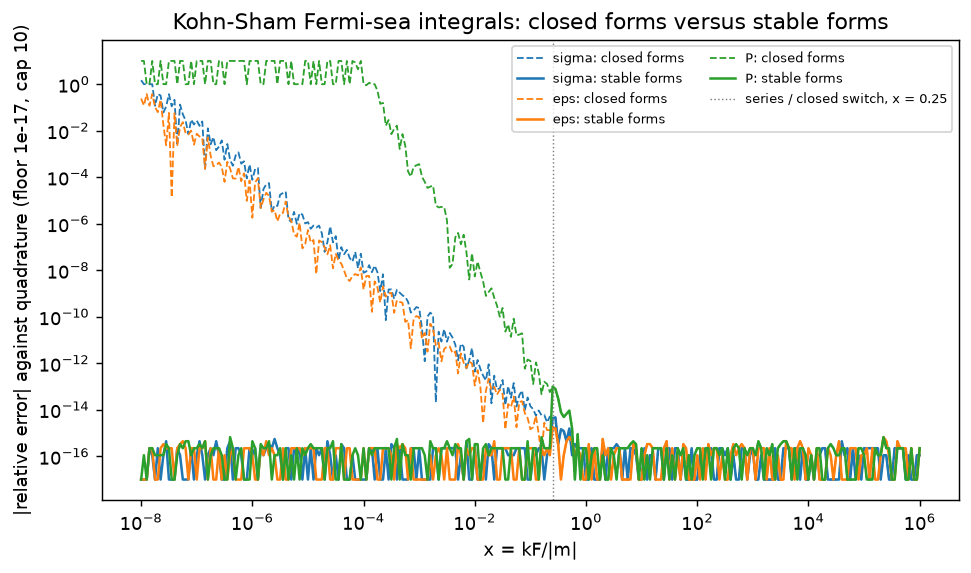
\includegraphics[width=0.9\linewidth]{nb05_ks_accuracy.png}
  \caption{\texttt{fable-cosmology/\allowbreak results/\allowbreak nb05\_ks\_accuracy.png} (notebook 05, section 5.1): the accuracy of
  the stable forms of the Fermi-sea integrals against adaptive quadrature, and of the closed forms.}
  \label{fig:nb05ks}
\end{figure}
\begin{figure}[tbp]
  \centering
  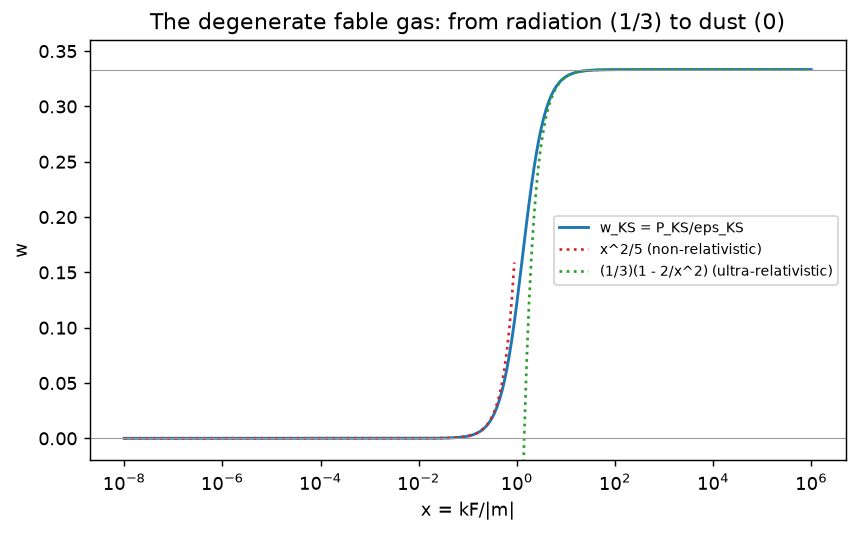
\includegraphics[width=0.75\linewidth]{nb05_w_ks.png}
  \caption{\texttt{fable-cosmology/\allowbreak results/\allowbreak nb05\_w\_ks.png} (notebook 05, section 5.2): $w_{\KS}(x)=\PKS/\epsKS$
  against $x=\kF/|m|$, from 0 (dust) to $1/3$ (radiation).}
  \label{fig:nb05wks}
\end{figure}

\subsection{The gap equation: uniqueness, branch selection, parameter domains}
\label{sec:7.3}

$f(m)=m-W'\bigl(\sigKS(m,\kF)/v\bigr)$. Since $\sigKS$ is odd and increasing in $m$ with slope
$\chi=d\sigKS/dm\leq\chi_0=g\kF^2/(4\pi^2)$, $f'=1-W''\chi/v$: the root is \textbf{unique} when $W''\leq0$
(attractive, concave $W$) or when $W''\chi_0/v<1$; otherwise there can be several roots [prose nb05 \S4;
file: \file{kohn_sham.rs}, module documentation]. Every potential states where its roots can lie and
whether the root is provably unique there (\cfcode{Potential::gap_plan} in \file{potentials.rs}). The
adopted parameter domains (design review DFT-16): \cfcode{expdamp} $m_0>0$, $s_1>0$ (the gap then pins
$0<\sigma<\min(n,s_1)$ strictly); \cfcode{power} $\lambda>0$, $0<\nu<1$, $\sigma$ in $(0,n)$ (the bare mass
$m_0$ may come out negative: \secref{sec:9.8}); \cfcode{quadratic} $\lambda<0$ unique, $\lambda>0$ all
roots enumerated.

\paragraph{Branch selection.} When several roots exist, the solver takes the one of \textbf{lowest}
energy density $\rho$ --- not the minimum of the Kohn--Sham energy $E_n[\sigma]$ over $\sigma$ in $(-n,n)$.
The no-sea functional is a minimax: its kinetic part $T_s=\epsKS(m(\sigma))-m(\sigma)\,\sigma$ is
\textbf{concave} ($d^2T_s/d\sigma^2=-1/\chi<0$), so the physical root is a \textbf{maximum} of $E_n$ over
$\sigma$, and its infimum is the variational collapse $E_n\to-|m_0|\,n$ as $\sigma\to-n$ (every particle
in the negative-mass band, i.e.\ in states of the Dirac sea). For attractive $W$ the auxiliary-field
\textbf{Walecka functional} $\Omega_n(m)=\epsKS(m)+W(\sigma_m)-m\,\sigma_m$, $W'(\sigma_m)=m$, is convex and
minimized at the gap root, with $\Omega_n(m^*)=\rho$. The numbers are in \secref{sec:8.1}.

\subsection{The energy--momentum tensor's expectation: \texorpdfstring{$\rho$, $P_{\mathrm{obs}}$, $P_{\mathrm{hid}}$}{rho, P\_obs, P\_hid}, and \texorpdfstring{$w$}{w}}
\label{sec:7.4}

On the gap:
\begin{align*}
  \rho&=3\PKS/v+W(\sigma_7) &&\text{(Section~29's trace identity $\varepsilon-3P=m\sigma$, per 7-volume)},\\
  \Pobs&=\PKS/v+\sigma_7W'-W,\\
  \Phid=\PC&=\sigma_7W'-W,\\
  \Pobs-\Phid&=\PKS/v\geq0 &&\text{(for every $W$: the Fermi gas can source}\\
  & &&\text{\phantom{(}$a_4''<0$, \secref{sec:4.6})},\\
  w_f&=\Pobs/\rho .
\end{align*}
The split $\rho=\rho_{\mathrm{qp}}+\rho_U$ with $\rho_{\mathrm{qp}}:=\epsKS/v$ (quasiparticles,
$w_{\mathrm{qp}}=\wDM=\PKS/\epsKS$ in $[0,1/3]$) and $\rho_U:=W-\sigma_7W'$ (the mean-field condensate,
with $P=-\rho_U$ along \textbf{all seven} spatial directions: an 8-dimensional vacuum energy that varies
with $\sigma$) is a \textbf{convention} [prose nb06 \S3; file: \file{kohn_sham.rs}].
\Secref{sec:7.10} defines the dark-matter and dark-energy equations of state built on it.

\subsection{Theorem: the Kohn--Sham fluid is exactly conserved in 8-dimensional Bianchi-I}
\label{sec:7.5}

The fable number in a comoving 7-volume, $(n_{\KS}/v)\,A^3v=n_{\KS}A^3$, is conserved, so $\kF=k_{F0}/A$.
Take $A$, $B$, $C$ and the mass $m(x_4)>0$ as \textbf{arbitrary} functions and $W$ arbitrary. Then,
identically,
\[
  \rho'+3H_A\,(\rho+\Pobs)+(3H_B+H_C)\,(\rho+\Phid)=\sigma_7\,\frac{d}{dx_4}\bigl[m-W'(\sigma_7)\bigr] .
\]
The right-hand side is the time derivative of the gap equation; on the self-consistent solution it
vanishes at every $x_4$, so the Kohn--Sham fluid obeys \secref{sec:5.5}'s conservation law (with
$\PC=\Phid$) \textbf{exactly}, for every $W$ --- the Einstein equations with this source are consistent.
The mechanism: $\rho+\Pobs=\wF\,n_{\KS}/v$ and $\rho+\Phid=\epsKS/v$ hold identically,
$d\varepsilon=\wF\,dn+\sigma\,dm$, and the gap cancels the $\sigma\,dm$ term against the variation of $W$.
Off the gap the fluid is \textbf{not} conserved. \cfproved{VIII \S33}
\begin{itemize}
  \item \cfL{CONSERVATION [definition]: the fable number per comoving 7-volume, (n\_KS/v) A\textasciicircum{}3 B\textasciicircum{}3 C, is constant when kF = kF0/A}
  \item \cfL{CONSERVATION [has content]: rho + P\_obs == wF n\_KS/v and rho + P\_hid == eps\_KS/v identically (no gap needed)}
  \item \cfL{CONSERVATION [THE RESULT]: rho' + 3 H\_A (rho + P\_obs) + (3 H\_B + H\_C)(rho + P\_hid) == sigma7 d/dx4[m - W'(sigma7)] IDENTICALLY, for arbitrary A, B, C, m(x4) > 0 and W: the KS fluid is exactly conserved on the gap}
  \item \cfL{CONSERVATION [control]: without the gap the fluid is NOT conserved -- the left side is not identically zero (witnessed on A = 1 + x4/2, B = 1 + x4/3, C = 1 + x4\textasciicircum{}2/3, m = 2 + x4, W = sigma\textasciicircum{}2, kF0 = 1, g = 8)}
\end{itemize}

The solver's form of the same law: $d\rho_8=\wF\,dn/v-(\varepsilon/v)\,d\ln v$, so at fixed $v$,
$d\rho_8/dn_8=\wF$ [file: \file{kohn_sham.rs}, module documentation]; its unit test
\file{kohn_sham::tests::thermodynamic_identities_at_the_self_consistent_point} and the end-to-end test
\file{covariant_conservation_along_real_fable8d_runs} check it [file: \file{kohn_sham.rs},
\file{tests/cosmology.rs}].

\subsection{The hidden-sheet driver}
\label{sec:7.6}

With $\PC=\Phid$, \secref{sec:5.4}'s evolution equations for $B$ and $C$ both read
\[
  H_B'+H_B\Theta=H_C'+H_C\Theta=\kappa F/6,\qquad F=\rho-3\Pobs+2\Phid .
\]
$F$ is the driver of the hidden sheet:
\begin{center}
\small
\renewcommand{\arraystretch}{1.3}
\begin{tabular}{@{}>{\raggedright\arraybackslash}p{0.52\linewidth}>{\raggedright\arraybackslash}p{0.42\linewidth}@{}}
\toprule
source & $F$\\
\midrule
radiation ($\Pobs=\rho/3$, $\Phid=0$) & $0$\\
dust & $\rho$\\
an 8-dimensional vacuum energy (all seven pressures $-\rho$; a bare $V_0$, the condensate $\rho_U$) & $2\rho$\\
the Kohn--Sham fable, on the gap & $2W-\sigma_7W'$ (off the gap: $\sigma_7(m-W')+2W-\sigma_7W'$)\\
the author's mass term $W=m_0\sigma$ & $m_0\sigma_7$ (like dust)\\
$W=V_0+m_0\sigma$ & $2V_0+m_0\sigma_7$\\
\bottomrule
\end{tabular}
\end{center}
\cfproved{VIII \S33}
\begin{itemize}
  \item \cfL{DRIVER [THE RESULT]: with P\_C = P\_hid, kappa (P\_hid - T/6) == kappa (P\_C - T/6) == kappa F/6, F = rho - 3 P\_obs + 2 P\_hid: the right-hand side of the B and C equations}
  \item \cfL{DRIVER [has content]: F == 0 for radiation, F == rho for dust, F == 2 rho for an 8D vacuum}
  \item \cfL{DRIVER [THE RESULT]: for the KS fluid F == sigma7 (m - W') + 2 W - sigma7 W' identically, i.e. F == 2 W - sigma7 W' on the gap; the mass term gives F == m0 sigma7 (dust-like), W = V0 + m0 sigma gives 2 V0 + m0 sigma7}
\end{itemize}

\subsection{Theorem: a frozen hidden sheet makes the fable radiation}
\label{sec:7.7}

Given $H_B=H_C=0$ at one time, the hidden sheet stays \textbf{frozen} for all time iff $F=0$ along the
history; for the Kohn--Sham fluid, for all $\sigma_7$ the history sweeps, iff $\sigma W'=2W$, i.e.
$W=c\,\sigma^2$. The gap is then $m=2c\,\sigma_7$, and $m=0$ is always a root. For $c<0$ it is the only one
($m\,\sigKS>0$ for $m\neq0$, so a root $m\neq0$ would give $m^2=2c\,(m\,\sigKS)/v<0$). For $c>0$ a
non-trivial root exists iff $c\,g\,\kF^2/(2\pi^2v)>1$ ($\sigKS/m$ decreases strictly, from $g\kF^2/(4\pi^2)$
at $m\to0$ to 0 at $m\to\infty$), and it has \textbf{higher} energy: on it
$\rho=\bigl(\epsKS(m)-m\,\sigKS(m)/2\bigr)/v$, and $\Delta(m)=\epsKS(m)-m\,\sigKS/2-\epsKS(0)$ vanishes at
$m=0^+$ with
\[
  \frac{d\Delta}{dm}=\frac{g\,m^3}{4\pi^2}\,\Bigl(\mathcal L-\frac{\kF}{\wF}\Bigr)>0
\]
($\mathcal L-\kF/\wF=\varphi(\kF/m)$, $\varphi(x)=\ln\bigl(x+\sqrt{1+x^2}\bigr)-x/\sqrt{1+x^2}$, which
vanishes at 0 and has derivative $x^2/(1+x^2)^{3/2}>0$). So the ground state of a frozen-compatible fable
is the $m=0$ branch, on which $\rho=\epsKS(\kF,0)/v$, $\Pobs=\rho/3$, $\Phid=0$: \textbf{radiation}. A
Kohn--Sham fable compatible with a frozen hidden sheet is neither dark matter nor dark energy.
\cfproved{VIII \S33}
\begin{itemize}
  \item \cfL{FROZEN [THE RESULT]: 2 W - sigma W' == 0 for all sigma iff W == c sigma\textasciicircum{}2 (the general solution of sigma W' == 2 W)}
  \item \cfL{FROZEN [has content]: m sigma\_KS > 0 for m > 0 (zero at kF = 0, kF-derivative g kF\textasciicircum{}2 m\textasciicircum{}2/(2 pi\textasciicircum{}2 wF) > 0; even in m, so also for m < 0); for c < 0 a root m != 0 of m = 2 c sigma\_KS/v would give m\textasciicircum{}2 = 2 c (m sigma\_KS)/v < 0: only m = 0}
  \item \cfL{FROZEN [has content]: phi(x) = Log[x + Sqrt[1 + x\textasciicircum{}2]] - x/Sqrt[1 + x\textasciicircum{}2] is 0 at x = 0 and increasing (derivative x\textasciicircum{}2/(1 + x\textasciicircum{}2)\textasciicircum{}(3/2)), hence positive for x > 0; and L - kF/wF == phi(kF/m)}
  \item \cfL{FROZEN [THE RESULT]: for c > 0, sigma\_KS/m decreases strictly (d/dm = -(g m/(2 pi\textasciicircum{}2))(L - kF/wF)) from g kF\textasciicircum{}2/(4 pi\textasciicircum{}2) at m -> 0 to 0 at m -> infinity: a non-trivial root of 1 = 2 c (sigma\_KS/m)/v exists iff c g kF\textasciicircum{}2/(2 pi\textasciicircum{}2 v) > 1}
  \item \cfL{FROZEN [THE RESULT]: on the non-trivial root (m = 2 c sigma7) rho == (eps\_KS - m sigma\_KS/2)/v, and Delta = eps\_KS(m) - m sigma\_KS/2 - eps\_KS(0) has Delta(0+) = 0 and dDelta/dm = (g m\textasciicircum{}3/(4 pi\textasciicircum{}2))(L - kF/wF) > 0: the m = 0 branch has LOWER rho}
  \item \cfL{FROZEN [has content]: witness numbers -- at g = 8, v = 1, c = 15, kF = 1 the non-trivial root m* exists (gap residual < 10\textasciicircum{}-20) and rho(m = 0) < rho(m*)}
  \item \cfL{FROZEN [THE RESULT]: on the m = 0 branch the frozen-compatible fable is RADIATION: rho = eps\_KS(kF, 0)/v, P\_obs = rho/3, P\_hid = 0}
\end{itemize}
The witness the run prints \cfdisplayed{VIII \S33}, \file{claude-fable/run_fermion_fable_part8.log}:
\begin{Verbatim}[fontsize=\scriptsize]
  frozen-compatible witness (g = 8, v = 1, c = 15, kF = 1): non-trivial root m* = 3.97853200077825223420767254928521681893`12.;  rho(m = 0) = 0.10132118364233777144387946320972763891`12.  <  rho(m*) = 0.28374208489508058306307225309709278221`12.
\end{Verbatim}

\subsection{The classical limit, and the sign rule}
\label{sec:7.8}

The classical limit is the \textbf{non-relativistic} limit $\kF\ll|m|$ (not a coherent zero mode: the
Pauli principle forbids that). Exactly, on the gap, with $s=H\sigma_7$ and $V(s):=W(s/H)$:
\[
  \rho=V(s)+3\PKS/v,\qquad \Pobs=s\,V'(s)-V(s)+\PKS/v,\qquad \Phid=s\,V'(s)-V(s),
\]
and as $\kF/m\to0$ ($m>0$), $\sigKS/n_{\KS}=1-\tfrac{3}{10}\,\kF^2/m^2+\dots$,
$(\epsKS-n_{\KS}m)/(n_{\KS}\kF^2/m)\to3/10$, $\PKS/(n_{\KS}\kF^2/m)\to1/5$: $\PKS/\rho\to0$ and the quantized
fluid reduces to Part~VI's $\rho=V(s)$, $P=s\,V'(s)-V(s)$ (its $K_h=0$ branch); $\Phid$ is exactly Part~VI's
on-shell pressure. With $s_0=n_{\KS}/v$, exactly on the gap,
\[
  \rho-W(s_0)=(\varepsilon-n\,m)/v-\bigl[W(s_0)-W(\sigma_7)-W'(\sigma_7)\,(s_0-\sigma_7)\bigr]:
\]
a second-order Taylor remainder in $s_0-\sigma_7$. \textbf{The sign rule:} $m\,\sigKS\geq0$, so on every
self-consistent solution $\operatorname{sign}(\sigma_7)=\operatorname{sign}(m)=\operatorname{sign}\bigl(W'(\sigma_7)\bigr)$;
for Part~VI's mass term $W=-2M\sigma$ the gap is $m=-2M$ and $\rho\to2|M|\,n/v>0$ --- the Part~VI branch
$Ms>0$, of negative energy, is not a self-consistent state. \cfproved{VIII \S33}
\begin{itemize}
  \item \cfL{CLASSICAL LIMIT [THE RESULT]: exactly, on the gap and with s = H sigma7, V(s) = W(s/H): rho == V(s) + 3 P\_KS/v, P\_obs == s V'(s) - V(s) + P\_KS/v, P\_hid == s V'(s) - V(s)}
  \item \cfL{CLASSICAL LIMIT [fidelity]: Section 24's on-shell P\_1 (cfP1Fable, re-checked here) is s V'(s) - V(s); evaluated at s = H sigma7 with V(s) = W(s/H) it IS the KS P\_hid = sigma7 W' - W}
  \item \cfL{CLASSICAL LIMIT [THE RESULT]: NR series (kF/m -> 0, m > 0): sigma\_KS/n\_KS = 1 - (3/10) kF\textasciicircum{}2/m\textasciicircum{}2 + ..., (eps\_KS - n\_KS m)/(n\_KS kF\textasciicircum{}2/m) -> 3/10, P\_KS/(n\_KS kF\textasciicircum{}2/m) -> 1/5}
  \item \cfL{CLASSICAL LIMIT [has content]: the design's form, exactly: on the gap (m = W'(sigma7) > 0) rho - W(s0) == (eps - n m)/v - [W(s0) - W(sigma7) - W'(sigma7)(s0 - sigma7)], s0 = n/v -- a second-order Taylor remainder in s0 - sigma7}
  \item \cfL{SIGN RULE [THE RESULT]: m sigma\_KS >= 0 gives sign(sigma7) == sign(m) == sign(W'(sigma7)); for Section 24's mass term W = -2 M sigma the gap is m = -2 M and W(sign(m) n/v) = -2 M sign(-2 M) n/v == 2 |M| n/v > 0}
\end{itemize}
Notebook 05 checks the series at $x=0.001$ and the sign at $m=-2$ \cfnb{nb05 \S5.4}:
\cfcode{(sigma/n - 1)/x^2 = -0.300000 (-3/10)}, \cfcode{(eps/(|m| n) - 1)/x^2 = +0.300000 (+3/10)},
\cfcode{P/(n kF^2/|m|) = 0.200000 (1/5)}; \cfcode{m = -2: sigma/n = -0.999999700: sgn(sigma) = sgn(m)}.

\subsection{\texorpdfstring{$w_f\geq-1$}{w\_f >= -1}: no phantom crossing}
\label{sec:7.9}

\[
  \rho+\Pobs=\wF\,n_{\KS}/v\geq0\qquad\text{so}\qquad w_f\geq-1\ \text{ wherever } \rho>0 .
\]
The quantized fermion fable \textbf{cannot cross the phantom divide}; the classical crossing of Part~VI
(\secref{sec:2.12.7}, at $V'(s^*)=0$) does not survive quantization. \cfproved{VIII \S33}
\cfL{PHANTOM [THE RESULT]: rho + P\_obs == wF n\_KS/v >= 0, so w\_f >= -1 wherever rho > 0 -- the quantized fable cannot cross the phantom divide}. Notebook 05 compared the classical $w_{\mathrm{cl}}=s\,V'/V-1$ of five of
Part~VI's potential shapes with the quantum $w=\Pobs/\rho$ of the lowest-energy gap root, over densities
$10^{-3}\leq n\leq30$ (in units where the classical $s$ equals $n$), for $W=\mathcal A\,V$ with
$\mathcal A=10^4,10^2,1$ --- a large $\mathcal A$ makes the quasiparticles heavy ($m=\mathcal A\,V'$), which
is the classical limit (915 points) \cfnb{nb05 \S5.4, file:
\file{fable-cosmology/results/nb05_classical_vs_quantum.csv}, figure \file{nb05_classical_vs_quantum.png}}
(figure~\ref{fig:nb05cq}):
\begin{center}
\small
\renewcommand{\arraystretch}{1.3}
\begin{tabular}{@{}>{\raggedright\arraybackslash}p{0.36\linewidth}>{\raggedright\arraybackslash}p{0.3\linewidth}>{\raggedright\arraybackslash}p{0.28\linewidth}@{}}
\toprule
potential ($V(s)$) & classical $\min w_{\mathrm{cl}}$ & quantum $\min w$ ($\mathcal A=10^4$, $100$, $1$)\\
\midrule
mass ($s$) & \texttt{+0.0000}, never crosses $-1$ & \texttt{+0.00000}, \texttt{+0.00000}, \texttt{+0.00741}\\
lambda-mass ($0.7+0.3\,s$) & \texttt{-0.9996}, never crosses $-1$ & \texttt{-0.99957}, \texttt{-0.99957}, \texttt{-0.99949}\\
power ($s+s^{0.236}$) & \texttt{-0.7601}, never crosses $-1$ & \texttt{-0.76012}, \texttt{-0.76012}, \texttt{-0.76012}\\
expdamp ($1.566+0.839\,s\,e^{-s/2.21}$) & \texttt{-1.3020}, \textbf{crosses $-1$} at $n=2.2047$ & \texttt{-0.99952}, \texttt{-0.99947}, \texttt{-0.99945}\\
lorentz ($1+s/(1+(s/1.5)^2)$) & \texttt{-1.2481}, \textbf{crosses $-1$} at $n=1.4999$ & \texttt{-0.99900}, \texttt{-0.99900}, \texttt{-0.99898}\\
\bottomrule
\end{tabular}
\end{center}
and it printed \cfcode{the quantum w >= -1 at every density, every A and every potential; the classical expdamp and lorentz cross -1}.
For \cfcode{expdamp} the gap keeps $0<\sigma<\min(n,s_1)$ strictly, with $\sigma\to s_1$ and $m\to0$ only as
$n\to\infty$ (solver test
\file{kohn_sham::tests::expdamp_pins_sigma_below_s1_and_mass_goes_to_zero_at_high_density}).

\begin{figure}[tbp]
  \centering
  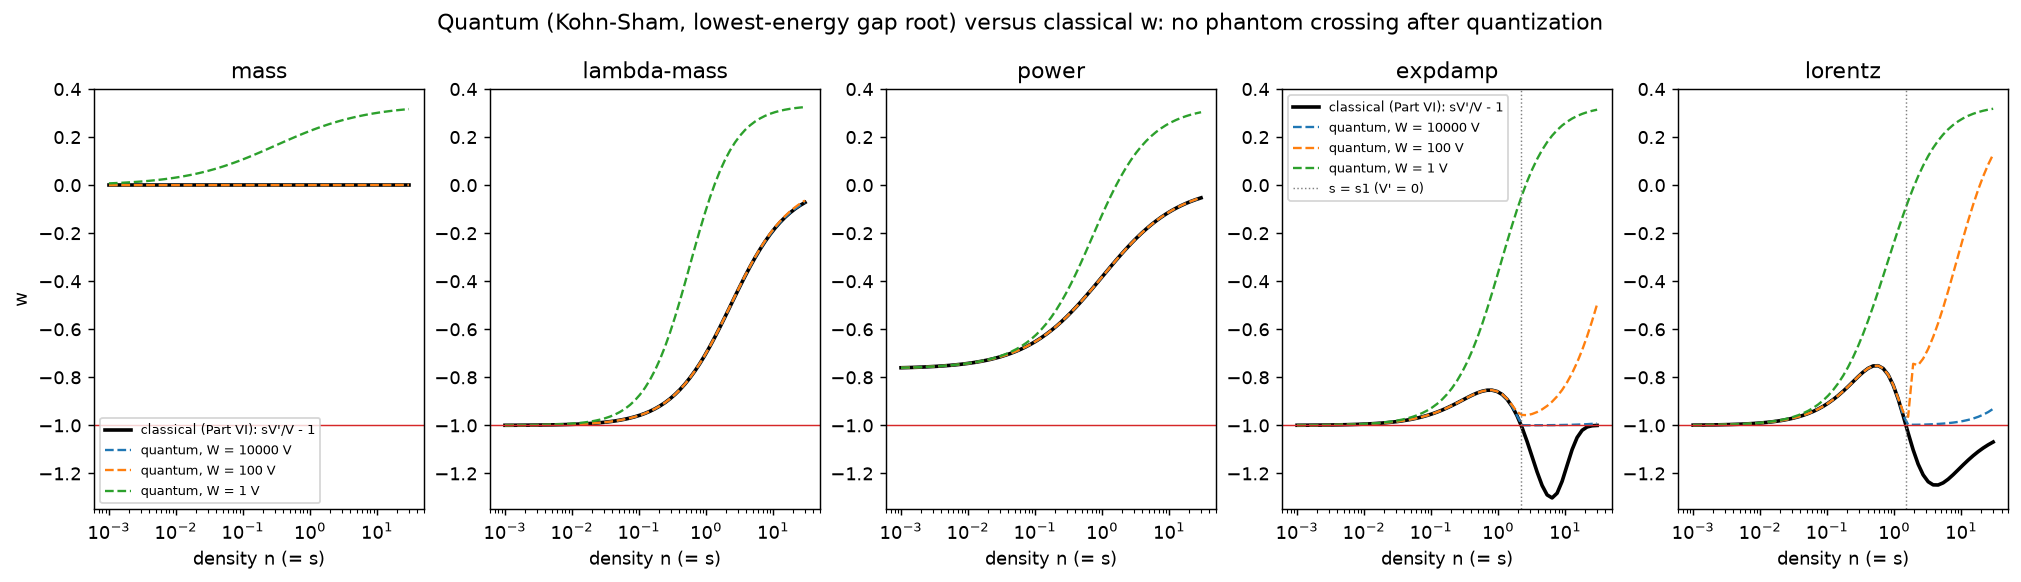
\includegraphics[width=0.95\linewidth]{nb05_classical_vs_quantum.png}
  \caption{\texttt{fable-cosmology/\allowbreak results/\allowbreak nb05\_classical\_vs\_quantum.png} (notebook 05, section 5.4): the
  classical $w_{\mathrm{cl}}=s\,V'/V-1$ against the quantum $w=\Pobs/\rho$ of the lowest-energy gap root.}
  \label{fig:nb05cq}
\end{figure}

\subsection{The equations of state an observer can define}
\label{sec:7.10}

Four definitions are used, and they must not be confused [file: \file{models.rs}, documentation of the
output columns; prose nb06 \S5]:
\begin{enumerate}
  \item $\boldsymbol{w_f=P_{\mathrm{obs},f}/\rho_f}$ --- the intrinsic equation of state of the whole fable
        fluid;
  \item $\boldsymbol{\wDM=w_{\mathrm{qp}}=\PKS/\epsKS}$ --- the intrinsic equation of state of the
        quasiparticles, in $[0,1/3]$;
  \item $\boldsymbol{\wDMeff=\wDM-\sigKS\,(dm/dN)/(3\epsKS)}$ --- the effective equation of state of the
        quasiparticles when the mass varies, which exchange energy with the condensate at the rate
        $Q=\sigma_8\,dm/dt$ (the exact exchange; $n\,dm/dt$ is its non-relativistic limit);
  \item $\boldsymbol{\wDE}$ --- the dark energy an observer \textbf{infers} by fitting cold dark matter plus
        dark energy: $\rhoDE=H_A^2-\Omega_{r0}A^{-4}-\Omega_{b0}A^{-3}-\mtoday\,n_{\mathrm{today}}A^{-3}$
        (radiation, baryons, and cold dark matter with \textbf{today's} mass $\meffx(A=1)$ subtracted),
        $\wDE=-1-\tfrac13\,d\ln\rhoDE/d\ln A$.
\end{enumerate}
The adiabatic sound speed of the fable is $c_s^2=(dP_{\mathrm{obs},f}/dN)/(d\rho_f/dN)$; $c_s^2<0$ is an
adiabatic instability. The split into dark matter and dark energy is a convention (\secref{sec:7.4}): the
condensate is an 8-dimensional vacuum energy.

\subsection{The vacuum energy of mass-varying potentials}
\label{sec:7.11}

For a constant mass the Dirac-sea energy is a constant; it is absorbed into $V$ and appears as a bare
cosmological constant. \textbf{The cosmological-constant problem is not solved here.} For a mass that
varies along the history the sea energy cannot be absorbed silently (design review DFT-4, adopted). The
renormalized one-loop Dirac-sea energy that the no-sea functional drops (relativistic Hartree
approximation, Chin 1977), per 3-volume, with reference mass $M$ and counterterms through $m^4$, is
\[
  \Evac(m)=-\frac{g}{16\pi^2}\Bigl[m^4\ln\frac mM+M^3(M-m)-\frac72M^2(M-m)^2+\frac{13}{3}M(M-m)^3-\frac{25}{12}(M-m)^4\Bigr]
\]
[file: \file{kohn_sham.rs}, function \cfcode{vacuum_energy}; its test
\file{kohn_sham::tests::vacuum_energy_vanishes_to_fifth_order_at_the_reference_mass}]. At $m=0$ the
bracket is $M^4\bigl(1-\tfrac72+\tfrac{13}{3}-\tfrac{25}{12}\bigr)=-M^4/4$, so
$\Evac(0)-\Evac(M)=g\,M^4/(64\pi^2)$ \cfderived. With $g=8$ and $\Ec=\rhoc^{1/4}=2.46261\times10^{-3}$\,eV
(asserted: \cfL{fable4d RUNS [definition]: the units computed from CODATA 2018 -- E\_c = rho\_c0\textasciicircum{}(1/4) == 2.46261e-3 eV, Omega\_r0 == 9.2096e-5, Omega\_b0 = 0.02237/h\textasciicircum{}2 == 0.049243 (to the quoted digits)}), a mass variation of order $m$ changes the vacuum energy by
\begin{gather*}
  \frac{g\,m^4/(64\pi^2)}{\rhoc}=3.44,\quad 3.44\times10^{4},\quad 3.44\times10^{8},\quad 3.44\times10^{12}\\
  \text{at } m=0.01,\ 0.1,\ 1,\ 10\ \text{eV}\qquad\text{(it scales as $m^4$)}
\end{gather*}
[derived here: $g/(64\pi^2)=0.012665$, $(m/\Ec)^4=271.9$ at $m=0.01$\,eV]. So for $m\gtrsim10$\,meV it
exceeds the critical density; notebook 05 prints the exact threshold \cfnb{nb05 \S5.8}:
\cfcode{Delta E_vac(0; M) = g M^4/(64 pi^2): check 1.000000000000003;  g M^4/(64 pi^2) exceeds rho_c0 for M > (64 pi^2/g)^(1/4) E_c = 7.341 meV},
and at $M=1$\,eV it gives $|\Evac|/\rhoc$ $=$ \texttt{2.760e-02}, \texttt{2.802e+03}, \texttt{9.454e+06},
\texttt{3.444e+08} at $m/M=0.99$, $0.9$, $0.5$, $0$ (the last is the $3.44\times10^{8}$ above); at
$M=1000$\,eV, \texttt{3.444e+20} at $m=0$; the fifth-order zero at $m=M$ is confirmed by the ratio
\texttt{31.9470} ($2^5=32$).

The design review's refinement (DFT-4, adopted): the sea energy \textbf{can} be absorbed formally by
reading $W$ as the fully renormalized effective potential, $\Omega(m)=\epsKS+\Evac+F$ $=$ no-sea with
$\tilde F=F+\Evac$; that reading is a \textbf{fine-tuning} of the bare potential against the sea energy.
The vacuum also adds $\sigma_{\mathrm{vac}}=d\Evac/dm$ to $\langle\bar\Psi\Psi\rangle$. The two options are
(a) to include $\Evac$ in $\rho$ and in the gap equation, or (b) to declare $W$ the renormalized
potential. \textbf{The runs use (b)}, and they print $\Evac(m(t))-\Evac(\mtoday)$ in units of $\rhoc$ (the
solver's column \cfcode{vac_over_rhoc}, $\Evac\bigl(\meffx;M=\meffx(A=1)\bigr)/v$). Along the power run
$\nu=0.236$, $\mtoday=30$\,eV notebook 05 found \cfnb{nb05 \S5.8} (figure~\ref{fig:nb05vac}):
\begin{Verbatim}[fontsize=\scriptsize]
power nu = 0.236, m_today = 30 eV: m_eff/m_today runs from 0.2007 (a = 1e-12) to 1;  max |solver vac_over_rhoc - formula| / (g M^4/(64 pi^2)) = 5.4e-15
   |Delta E_vac(m(t)) - Delta E_vac(m_today)| / rho_total: max over a >= 0.3 = 1.314e+13,  at a = 0.5: 1.149e+13
\end{Verbatim}
\Secref{sec:9.6} gives the ratio for every run.

\begin{figure}[tbp]
  \centering
  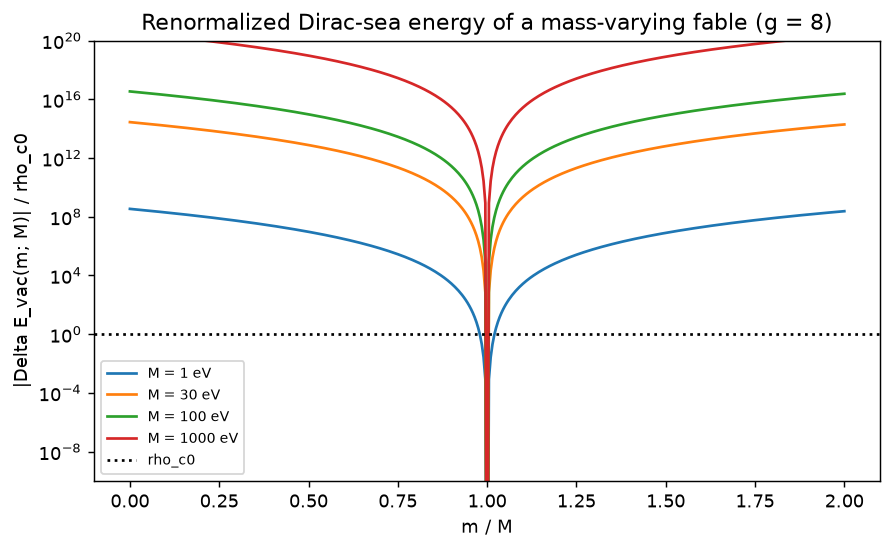
\includegraphics[width=0.9\linewidth]{nb05_vacuum_energy.png}
  \caption{\texttt{fable-cosmology/\allowbreak results/\allowbreak nb05\_vacuum\_energy.png} (notebook 05, section 5.8): the
  renormalized Dirac-sea energy of a mass-varying fable.}
  \label{fig:nb05vac}
\end{figure}

\subsection{Exchange and correlation}
\label{sec:7.12}

The Kohn--Sham functional of \secref{sec:8.1} has $E_{\mathrm{xc}}$ neglected (the Hartree mean field). For
the author's mass term ($W$ linear) the action is bilinear, the theory is free, and the mean field is
\textbf{exact} ($E_{\mathrm{xc}}=0$). For a nonlinear $W$ the design review (DFT-14) estimated that the Fock
exchange of the contact interaction is suppressed relative to the Hartree term by $\sim1/g=1/8$ only in
the non-relativistic regime $\kF\ll m$, and is of order one or larger for $\kF\gtrsim m$; in the
relativistic era its neglect is controlled only by the smallness of the interaction energy relative to
$3\PKS$. That ratio was not computed in the runs; the neglect of $E_{\mathrm{xc}}$ is a stated
approximation of every mass-varying result on this page.

% ===============================================================================================
\section{Density-functional theory: the fable ground and first excited states}
\label{sec:8}

The author asked to ``use some of the relevant ideas from Density Functional Theory to obtain the fable
ground and first excited states''. Two systems are treated: the \textbf{homogeneous} fable gas of the
present universe (sections~\ref{sec:8.1}--\ref{sec:8.2}), and the fable \textbf{along the hidden
coordinate $x_0$} of the primordial field, where the wall $x_0=0$ binds discrete states
(sections~\ref{sec:8.3}--\ref{sec:8.7}). The homogeneous numbers are printed by notebook 05
\cfnb{nb05 \S5.5, \S5.6}; the wall-state numbers are quoted from
\file{fable-cosmology/fermion/waveguide_REPORT.txt} \cfnb{WG n} and its logs, and notebook
\file{07_fable_dft_states.ipynb} is the notebook that reproduces them (each number it must re-confirm
carries a re-confirmation mark). The development logs that the report names are files under
\file{fable-cosmology/fermion/dev/}, a folder the repository ignores; the report, which is tracked, quotes
them.

\subsection{The functional, and the homogeneous Kohn--Sham ground state}
\label{sec:8.1}

\paragraph{The functional.} For the conserved charge $n$ and the scalar density $\sigma$ (the
relativistic Hohenberg--Kohn--Sham scheme; the Serot--Walecka mean field is its Hartree limit), the
energy of the gas at fixed $n$ is
\begin{gather*}
  E_n[\sigma]=T_s(\sigma;n)+W(\sigma)+E_{\mathrm{xc}},\qquad T_s=\epsKS\bigl(m(\sigma)\bigr)-m(\sigma)\,\sigma,\qquad
  \sigKS\bigl(m(\sigma),\kF\bigr)=\sigma,\\
  \frac{dE_n}{d\sigma}=W'(\sigma)-m(\sigma)\quad\text{(stationary exactly at the gap roots)},\qquad
  \frac{d^2T_s}{d\sigma^2}=-\frac1\chi<0,
\end{gather*}
with $E_{\mathrm{xc}}$ neglected (\secref{sec:7.12}) and the Dirac sea excluded (the no-sea functional; its
energy is \secref{sec:7.11}). The Kohn--Sham Slater determinant is the filled Dirac sea (renormalized
away) plus the Fermi sea $|k|<\kF$ of the lowest positive band. \textbf{The ground state is the stationary
point of this minimax functional} --- a maximum in $\sigma$ and a minimum in the occupations --- and
\textbf{never} its minimum over $\sigma$ [prose nb05 \S5.6; solver: design departure D1 of the
development report, and the unit tests
\file{kohn_sham::tests::ks_functional_stationary_point_is_a_maximum_for_the_mass_term},
\file{walecka_functional_is_minimized_at_the_gap_root},
\file{multiple_gap_roots_are_found_and_the_lowest_energy_one_is_taken} in \file{kohn_sham.rs}]. For
linear $W$ the theory is free, $m=m_0$ exactly, and the Kohn--Sham state is the exact ground state.

\paragraph{The minimax, in numbers} \cfnb{nb05 \S5.6, file: \file{fable-cosmology/results/nb05_minimax.csv},
figure \file{nb05_minimax.png}} (figure~\ref{fig:nb05minimax}):
\begin{Verbatim}[fontsize=\scriptsize]
mass term W = 2 sigma, kF = 1.5: n = 0.4559453264, the gap root sigma* = 0.3961298703 (sigma*/n = 0.868810)
E_n(sigma*) = 1.052962422118 = rho = eps_KS(m0) = 1.052962422118;  max of E_n over the grid = 1.052959281278
E_n/n at sigma = -(1 - 1e-7) n: -1.999480  (the collapse value -|m0| = -2.0)

attractive W = sigma - 10 sigma^2, kF = 1: unique gap root m* = 0.2112489356, rho = 0.1211932853;  Omega_n(m*) = 0.121193285306
Omega_n on the grid: minimum 0.121193451922 at m = 0.2100;  second differences all positive (convex): True
\end{Verbatim}
The root of the mass term is the \textbf{maximum} of $E_n$ (the grid maximum lies just below it), and
$E_n/n$ falls to the collapse value $-|m_0|$ as $\sigma\to-n$. For the attractive $W$ the convex Walecka
functional $\Omega_n(m)=\epsKS(m)+W(\sigma_m)-m\,\sigma_m$ has its minimum at the gap root, equal to $\rho$.

\paragraph{Several roots, and a first-order transition.} For the repulsive
$W=m_0\sigma+(\lambda/2)\,\sigma^2$ with $(m_0,\lambda)=(0.05,20)$ at $\kF=1$,
$W''\chi_0=\lambda\,g\,\kF^2/(4\pi^2)=4.0528>1$ and there are three roots; the Rust solver's \cfcode{gap}
command and the Python solver agree \cfnb{nb05 \S5.5}:
\begin{Verbatim}[fontsize=\scriptsize]
# potential Quadratic { v0: 0.0, m0: 0.05, lam: 20.0 }, kF = 1e0, v = 1e0, n8 = 1.3509491152311703e-1, plan = Scan { lo: -2.651898230462341, hi: 2.7518982304623405 }
m,sigma8,rho8,P_obs,P_hid,gap_residual
-2.535353916022531e0,-1.292676958011266e-1,1.909782056219713e-1,1.772147779888931e-1,1.671013717773260e-1,8.506e-17
-1.640336879334347e-2,-3.320168439667173e-3,1.012381942988485e-1,3.387489103006236e-2,1.102351846776195e-4,-1.898e-17
2.644093986040535e0,1.297046993020268e-1,2.039272771420881e-1,1.779694075325236e-1,1.682330902102918e-1,0.000e0
# selected (Lowest): m = -1.640336879334347e-2, rho8 = 1.012381942988485e-1, roots = 3
\end{Verbatim}
with $(\rho+P)/(\wF n)=$ \texttt{1.000000000000} on every root (so $w\geq-1$ on every branch), and
\cfcode{uniqueness criterion lam chi0 < 1 holds for kF < 0.4967; three roots first appear at kF = 0.625 on this grid; the ground state jumps from m = +0.4756 (kF = 0.600) to m = -0.0998 (kF = 0.625)}
\cfnb{nb05 \S5.5, figure \file{nb05_gap_roots.png}} (figure~\ref{fig:nb05gap}): the ground state jumps
between branches --- a first-order transition. That is why the solver refuses a repulsive quadratic run
(\secref{sec:9.11}): energy conservation across the jump would need a Maxwell construction, which it does
not implement.

\begin{figure}[tbp]
  \centering
  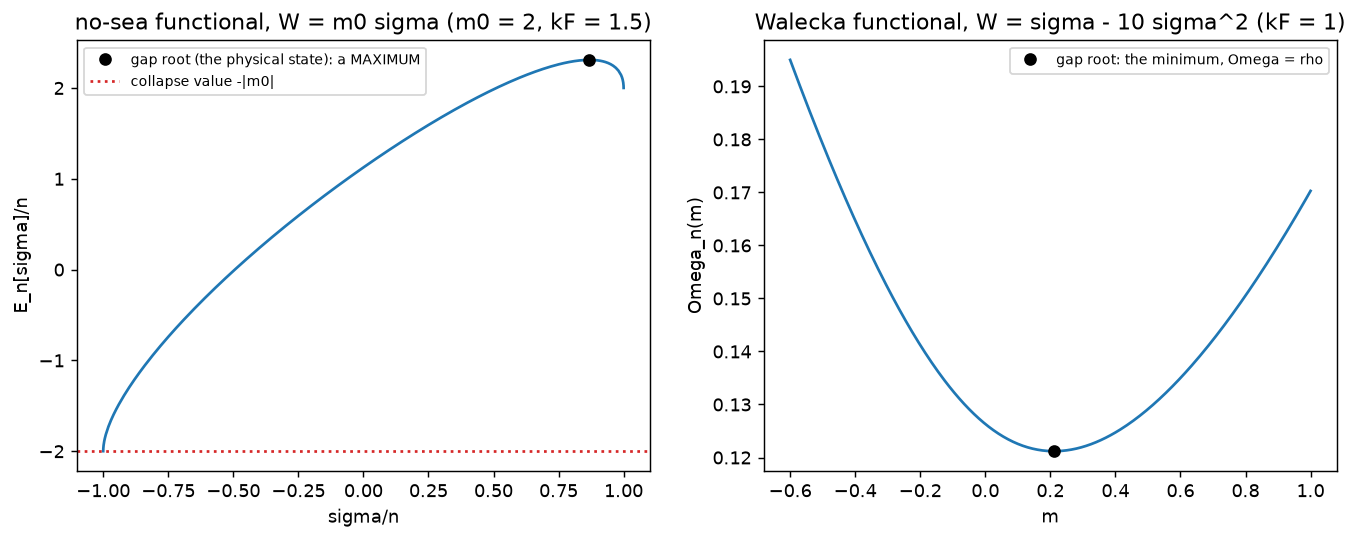
\includegraphics[width=0.95\linewidth]{nb05_minimax.png}
  \caption{\texttt{fable-cosmology/\allowbreak results/\allowbreak nb05\_minimax.png} (notebook 05, section 5.6): the no-sea
  Kohn--Sham functional $E_n[\sigma]$ of the mass term (its gap root is a maximum) and the Walecka
  functional $\Omega_n(m)$ of an attractive $W$ (its gap root is a minimum).}
  \label{fig:nb05minimax}
\end{figure}
\begin{figure}[tbp]
  \centering
  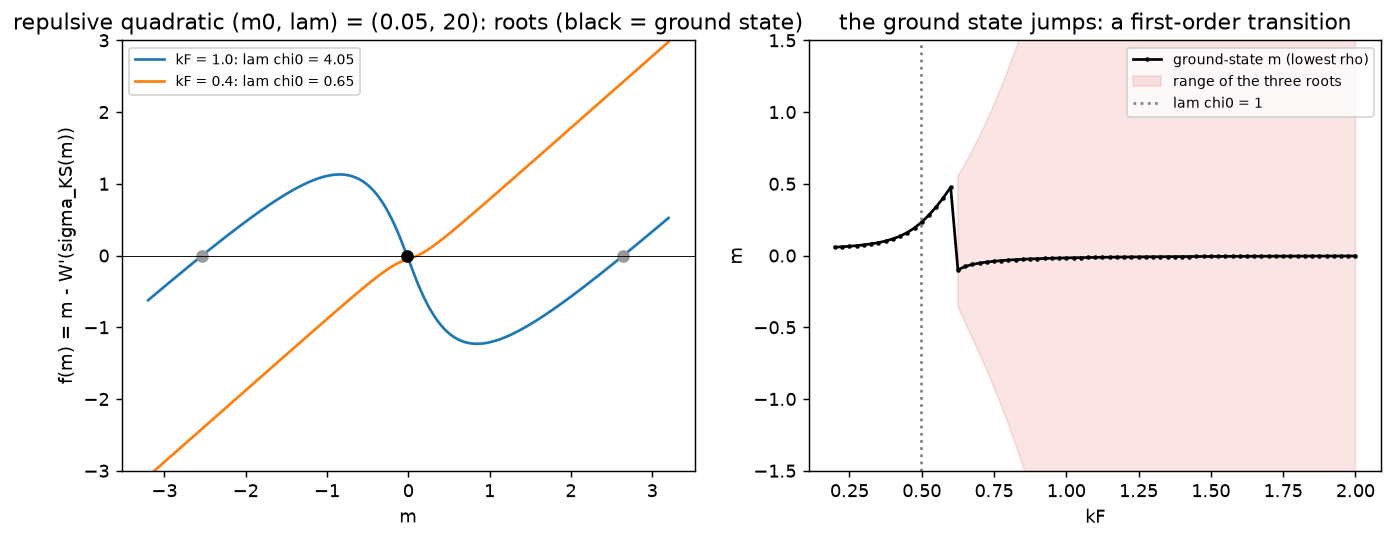
\includegraphics[width=0.95\linewidth]{nb05_gap_roots.png}
  \caption{\texttt{fable-cosmology/\allowbreak results/\allowbreak nb05\_gap\_roots.png} (notebook 05, section 5.5): the roots of the
  gap equation of the repulsive quadratic $W$ against $\kF$, and the jump of the ground state between
  branches.}
  \label{fig:nb05gap}
\end{figure}

\subsection{The first excited states of the homogeneous gas}
\label{sec:8.2}

The design review (DFT-15, adopted) states them; they are not assertions of the notebook, and the
derivation is short \cfderived:
\begin{itemize}
  \item \textbf{Particle--hole excitations} (a quasiparticle moved from just inside to just outside the
        Fermi surface) are \textbf{gapless}: $\Delta E\to0$ as the momentum transfer goes to zero. The
        lowest excited state of the gas is degenerate with the ground state in the thermodynamic limit,
        and it has no effect on $w$.
  \item \textbf{Pair excitations} create a particle above the Fermi sea (energy $\geq\wF$, momentum
        $|k_1|\geq\kF$) and a hole in the Dirac sea, an antiparticle (energy $\sqrt{k_2^2+m^2}\geq|m|$), with
        total momentum $q=k_1+k_2$. At $q=0$, $k_2=-k_1$, and the threshold is $2\wF$ (Pauli blocking
        pushes it from $2|m|$ to $2\wF$). The absolute threshold is $\wF+|m|$, at $|q|=\kF$ ($|k_1|=\kF$,
        $k_2=0$).
  \item \textbf{Delta-SCF} (moving one quantum and re-solving the gap): in the homogeneous gas one quantum
        changes $\sigma$ by $O(1/\text{volume})$, so the self-consistent excitation energy of one quantum
        equals the single-particle one. A finite effect needs a finite fraction of the particles, which is
        how the wall problem below defines its first excited state (design review DFT-9).
\end{itemize}

\subsection[{The states along the hidden coordinate: the problem [WG 2]}]{The states along the hidden coordinate: the problem \cfnb{WG 2}}
\label{sec:8.3}

The wall-state solver works at fixed observer's time on the canonical frame, with $a_4$ frozen to a
constant (the adiabatic approximation). The spectrum depends on the transverse momentum $k$ and the frozen
$a_4$ only through $K_\infty=k\,e^{a_4}$, so every number below is a function of $K_\infty$; the code works
with $K_\infty$ directly (internally it sets the frozen constant to zero, which only identifies $k$ with
$K_\infty$; nothing here or in the notebook gives $a_4$ a value). Units: $H=1$, $\hbar=c=1$. Its
derivation, \file{fable-cosmology/fermion/waveguide_derivation.wls}, loads the notebook's own Input cells
1--117 (with \cfcode{DumpSave} blocked) and uses only the notebook's objects (\cfcode{T16},
\cfcode{sigma16}, \cfcode{gammaCurvedCanonical}, \cfcode{GammaSpinCanonical}, \cfcode{cfDcov16},
\cfcode{gCanonical}, \cfcode{RicciScalarCanonical}, \cfcode{eta4488}); its log records
\cfcode{94 checks, 94 PASS, 0 FAIL} in 171.4\,s, and that the notebook's own 142 assertions of cells
1--117 passed while loading [file: \file{fable-cosmology/fermion/waveguide_derivation.log}].

\paragraph{The reduction.} With $\Psi=e^{ikx_1-i\omega x_4}\sqrt{\sin 6Hx_0}\;\Psi'(x_0)$ the Dirac equation
$\gamma^\mu D_\mu\Psi=m\Psi$ ($m=H\,V'(s)$; $m=-2M$ for the author's mass term) becomes \textbf{exactly}
\begin{gather*}
  (\gamma^\mu D_\mu-m)\,\Psi=\sqrt{\sin}\;e^{(\dots)}\Bigl[\cot\,T_0\,\partial_0+i\,k\,e^{A_4}\sin^{1/6}\,T_1-i\,\omega\,T_4-m\Bigr]\Psi',\\
  T_0\,\partial_z\Psi'+i\,K(z)\,T_1\Psi'-i\,\omega\,T_4\Psi'=m\,\Psi',\qquad
  K(z)=K_\infty\bigl(1-e^{-12Hz}\bigr)^{1/12},\qquad K_\infty=k\,e^{a_4}
\end{gather*}
in the proper distance $z=-\ln\cos(6Hx_0)/(6H)$ ($\cot\,d/dx_0=d/dz$; $z=0$ at the wall, a finite proper
distance away; $z\to\infty$ as $6Hx_0\to\pi/2$). The measure is
$\sqrt{|g|}\,|\Psi|^2dx_0=|\Psi'|^2dz$, so the one-particle space is $L^2(dz)$. The transverse term rises
from $K(0)=0$ at the wall ($K=K_\infty(12Hz)^{1/12}(1-Hz/2+\dots)$, $K'$ integrable) to $K_\infty$: a
``pocket'' of width $\sim1/(12H)$ ($K^2/K_\infty^2=0.875776$, $0.942018$, $0.984275$ at $z=0.05$, $0.1$,
$0.2/H$). The wall is a curvature singularity at finite proper distance: $R\,z^2\to-31/24$ as $z\to0$.

\paragraph{Hamiltonian form and the $2\times2$ blocks.} $\omega\,\phi=h\,\phi$,
$h=-i\,\alpha_z\,\partial_z+K(z)\,\alpha_x+m\,\beta$ with $\alpha_z=-T_4T_0$, $\alpha_x=-T_4T_1$,
$\beta=-i\,T_4$ (Hermitian involutions, pairwise anticommuting); $J=-i\,T_0T_1T_2T_3T_4$ commutes with $h$.
$w_3=\alpha_z\alpha_x\beta$ ($w_3^2=-1$) is central; the algebra $\langle\alpha_z,\alpha_x,\beta,J\rangle$ has
dimension 16, and $\mathbb C^{16}$ splits into \textbf{8 invariant 2-dimensional blocks}: 4 with $w_3=-i$
($J=+1$ twice, $J=-1$ twice) and 4 with $w_3=+i$. In an explicit block basis every block has
$\alpha_z=\sigma_y$, $\beta=\sigma_z$, $T_0=\sigma_x$, and with $\phi=(f,g)$:
\begin{align*}
  \text{irrep } w_3=-i:&\qquad f'=-K(z)\,f+(m+\omega)\,g,\qquad g'=K(z)\,g+(m-\omega)\,f,\\
  \text{irrep } w_3=+i:&\qquad \text{the same with } K\to-K .
\end{align*}

\paragraph{The wall conditions.} The self-adjoint conditions of a block are exactly the real lines
$f(0)\cos\vartheta+g(0)\sin\vartheta=0$, $\vartheta$ in $[0,\pi)$, and all of them have zero normal current.
Only $\vartheta=\pm\pi/4$ give $\bar\Psi\Psi=0$ at the wall, and only they are covariant under the wall's
Spin(1,3) of $x_1..x_4$: the MIT (bag) conditions $\Tsix{0}\,\Psi=\pm\Psi$ (MIT$+$: $f=g$; MIT$-$: $f=-g$ in
the basis above). The complete covariant, $J$-preserving family is $P\,\Psi(0)=\Psi(0)$ with
$P=\Tsix{0}\,Q$, $Q$ any Hermitian involution in the 8-dimensional commutant of the Clifford algebra of
$\Tsix{0..4}$ (which contains $J$); all of them have zero normal current and $\bar\Psi\Psi=0$. Flavour
symmetry ($Q$ central: $\pm1$, $\pm J$) together with charge conjugation ($P$ real) select $Q=\pm1$, the
uniform MIT walls; a mixed $Q$ gives one MIT$+$ sector and one MIT$-$ sector with halved multiplicities.
Without $J$-preservation there are more, e.g.\ $P=T_0\exp(i\,v_t\,T_0T_5)$. A \textbf{same-sign} wall is
$\Tsix{0}\,\Psi=\operatorname{sign}(m)\,\Psi$ (the limit of an outside mass of the same sign); an
\textbf{opposite-sign} wall is $\Tsix{0}\,\Psi=-\operatorname{sign}(m)\,\Psi$ (a domain wall); for the
author's mass term $m=-2M$, so both are physically possible.

\paragraph{The structure of the spectrum.} With MIT walls the 16-component spectrum at transverse momentum
$K$ is $S(K)=A(K)\cup\bigl(-A(K)\bigr)$, $A(K)$ the levels of the $w_3=-i$ block equation, symmetric under
$\omega\to-\omega$; a positive level is \textbf{4-fold} per transverse momentum vector (two blocks with
$J=+1$, two with $J=-1$, of one irrep), and 8-fold only when $\omega$ and $-\omega$ both lie in $A(K)$. The
8 states per momentum of the homogeneous gas split at the wall into two generally non-degenerate 4-fold
branches. The bulk continuum is $|\omega|\geq R=\sqrt{m^2+K_\infty^2}$; $z=0$ is a regular (limit-circle)
endpoint and $z\to\infty$ limit point. Second-order form: $f''=\bigl(K^2-K'+m^2-\omega^2\bigr)f$, a
supersymmetric pair with superpotential $K$; for $K>0$ the $f$-channel has the attractive pocket $-K'$.

\paragraph{Exact solutions} (used for validation): constant $K$, MIT$-$: $\omega=-K$, $\phi=e^{-mz}(1,-1)$;
the true profile with $g(0)=0$: $\omega=m$ for \textbf{every} $K_\infty>0$ (a flat band); constant $K$, any
$\vartheta$: a level $\omega=-(m\cos2\vartheta+K\sin2\vartheta)$ exists iff
$\kappa=m\sin2\vartheta-K\cos2\vartheta>0$; constant $K>0$, MIT$+$: \textbf{no} level.

\subsection[{Numerical method and its validation [WG 3, WG 5]}]{Numerical method and its validation \cfnb{WG 3, WG 5}}
\label{sec:8.4}

The block problem is solved by the Pr\"ufer angle $(f,g)=r\,(\cos p,\sin p)$,
$p'=m\cos2p+K\sin2p-\omega$, $p(0)=\vartheta+\pi/2$, matched to the exact decaying direction of the
constant-coefficient problem beyond $z_a=3/H$ (where $K(z)/K_\infty-1<2\times10^{-17}$). The mismatch
$\Delta(\omega)$ is strictly decreasing in $\omega$, so the number of levels in the gap is exactly
$\#\{\,j:\Delta(+R)<j\pi<\Delta(-R)\,\}$ --- a rigorous count that catches shallow levels. Roots are found on
a logarithmic grid of the decay rate $\kappa$ and refined by Brent's method; two integrators (adaptive
DOP853 at $10^{-12}$, and a 4th-order Magnus propagator) are compared. \cfcode{python waveguide.py validate}
runs 64 checks, all PASS (log \file{dev/waveguide_run_validate.log}, quoted in \file{waveguide_REPORT.txt}
\S3), among them: the exact solutions above (errors $\leq6\times10^{-16}$); Hellmann--Feynman for the scalar
density ($d\omega/dm=\int(f^2-g^2)\,dz$, agreement $3\times10^{-8}$); the full $16\times16$ system with the
notebook's \cfcode{T16}, in which every level has multiplicity exactly 4; and the small-$K$ slope of the
edge band against its closed form $\omega/K_\infty\to-\frac{m}{6H}\,B\bigl(\frac{m}{6H},\frac{13}{12}\bigr)$ ($B$
the Euler beta function): \texttt{-0.980822728} vs \texttt{-0.980822733} at $m=H$.

The independent Mathematica check \file{fable-cosmology/fermion/waveguide_check.wls} (a different language,
\cfcode{NDSolve} at 30 digits, the normalized Wronskian with \cfcode{FindRoot}, \cfcode{NullSpace} for the
asymptotic data) reports \cfcode{11 checks, 11 PASS, 0 FAIL} and agreement with the Python levels to at
most \texttt{4.68e-11} \cfnb{WG 5}. Its level table:

{\small
\begin{center}
\begin{tabular}{@{}>{\raggedright\arraybackslash}p{0.31\linewidth}>{\raggedright\arraybackslash}p{0.25\linewidth}>{\raggedright\arraybackslash}p{0.27\linewidth}l@{}}
\toprule
case & \file{waveguide.py} & Mathematica & difference \tabularnewline
\midrule
same-sign $K=80$, $n=0$ (irrep $-i$) & \texttt{70.985307229908} \texttt{\{\{NB07\}\}} & \texttt{70.98530722995475448906} & \texttt{4.68e-11} \tabularnewline
same-sign $K=80$, $n=1$ (irrep $+i$) & \texttt{78.1442493324274} \texttt{\{\{NB07\}\}} & \texttt{78.14424933243057439331} & \texttt{3.17e-12} \tabularnewline
same-sign $K=80$, $n=2$ (irrep $-i$) & \texttt{79.3714957790936} \texttt{\{\{NB07\}\}} & \texttt{79.37149577909911904082} & \texttt{5.51e-12} \tabularnewline
same-sign $K=80$, $n=3$ (irrep $+i$) & \texttt{79.9873085520475} \texttt{\{\{NB07\}\}} & \texttt{79.98730855204863978335} & \texttt{1.15e-12} \tabularnewline
same-sign $K=8$, shallow (irrep $-i$) & \texttt{8.05383822789729} \texttt{\{\{NB07\}\}} & \texttt{8.053838227898042799445} & \texttt{7.53e-13} \tabularnewline
same-sign $K=40$, $n=1$ (irrep $+i$) & \texttt{39.9665602657784} \texttt{\{\{NB07\}\}} & \texttt{39.96656026577953705636} & \texttt{1.14e-12} \tabularnewline
opposite-sign $K=3$, edge (irrep $-i$) & \texttt{-2.93849067695725} \texttt{\{\{NB07\}\}} & \texttt{-2.938490676960405133909} & \texttt{3.16e-12} \tabularnewline
opposite-sign $K=3$, edge (irrep $+i$) & \texttt{2.9384906769572} \texttt{\{\{NB07\}\}} & \texttt{2.938490676960405133909} & \texttt{3.21e-12} \tabularnewline
$g(0)=0$, $K=3$, flat band (irrep $-i$) & \texttt{1.} \texttt{\{\{NB07\}\}} & \texttt{1.000000000000000000000} & \texttt{0} \tabularnewline
$\vartheta=1.0$, $K=3$ (irrep $-i$) & \texttt{-2.21043470304386} \texttt{\{\{NB07\}\}} & \texttt{-2.210434703050103980776} & \texttt{6.24e-12} \tabularnewline
same-sign $m=4$, $K=20$ (irrep $-i$) & \texttt{20.1427411133772} \texttt{\{\{NB07\}\}} & \texttt{20.14274111338139405878} & \texttt{4.20e-12} \tabularnewline
\bottomrule
\end{tabular}
\end{center}
}

It also confirms the 4-fold multiplicities in the full 16-component system (four singular values below
$10^{-3}$ of the fifth, rising at $\omega\pm d\omega$) and the thresholds $K_c(1)=6.70624065181$ and
$K_c(2)=33.9189585083$ (the Pr\"ufer mismatch crosses an integer multiple of $\pi$ between
$(1-10^{-6})\,K_c$ and $(1+10^{-6})\,K_c$). At $K=80$ \cfcode{NDSolve} on the $16\times8$ matrix system did not
finish within 30 minutes, so there the $16\times16$ check uses an independently written
Magnus/\cfcode{MatrixExp} propagator.

\subsection[{The wall levels: ground and first excited states, in tables [WG 4]}]{The wall levels: ground and first excited states, in tables \cfnb{WG 4}}
\label{sec:8.5}

All at $m=H=1$ unless stated; the levels are the \textbf{positive} levels of the full 16-component problem,
each 4-fold per transverse momentum vector.

\paragraph{Thresholds of the same-sign wall} (the transverse momentum $K_c(n)$ at which the $n$-th positive
level appears; exact count, bisection to $10^{-9}$; \file{dev/waveguide_run_threshold.log}):

{\small
\begin{center}
\begin{tabular}{@{}lllllll@{}}
\toprule
$m/H$ & $K_c(1)/H$ & irrep & $K_c(1)/m$ & $K_c(2)/H$ & irrep & $K_c(2)/m$ \tabularnewline
\midrule
0.25 & \texttt{3.39259952} \texttt{\{\{NB07\}\}} & $-i$ & \texttt{13.57040} & \texttt{33.87815035} \texttt{\{\{NB07\}\}} & $+i$ & \texttt{135.51260} \tabularnewline
0.50 & \texttt{4.77916520} \texttt{\{\{NB07\}\}} & $-i$ & \texttt{9.55833} & \texttt{33.89177761} \texttt{\{\{NB07\}\}} & $+i$ & \texttt{67.78356} \tabularnewline
1.00 & \texttt{6.70624065} \texttt{\{\{NB07\}\}} & $-i$ & \texttt{6.70624} & \texttt{33.91895851} \texttt{\{\{NB07\}\}} & $+i$ & \texttt{33.91896} \tabularnewline
2.00 & \texttt{9.33759991} \texttt{\{\{NB07\}\}} & $-i$ & \texttt{4.66880} & \texttt{33.97299731} \texttt{\{\{NB07\}\}} & $+i$ & \texttt{16.98650} \tabularnewline
4.00 & \texttt{12.80358979} \texttt{\{\{NB07\}\}} & $-i$ & \texttt{3.20090} & \texttt{34.07956537} \texttt{\{\{NB07\}\}} & $+i$ & \texttt{8.51989} \tabularnewline
8.00 & \texttt{17.04604924} \texttt{\{\{NB07\}\}} & $-i$ & \texttt{2.13076} & \texttt{34.28513351} \texttt{\{\{NB07\}\}} & $+i$ & \texttt{4.28564} \tabularnewline
\bottomrule
\end{tabular}
\end{center}
}

The first level always appears in irrep $-i$, with $K_c(1)$ growing roughly like $6.7\,(m/H)^{1/2}H$; the
second always in the other irrep, at $K_c(2)=33.9$--$34.3\,H$, almost independent of $m$. Within irrep $-i$
alone the second level appears only at $K=$ \texttt{49.540216755} \texttt{\{\{NB07\}\}} ($m=H$).
\textbf{For $K<K_c(1)$ there is no bound level at all} --- the design's first guess (``for $k\neq0$ the wall
region is a potential pocket: bound states below $\sqrt{m^2+k^2e^{2a_4}}$'') was refuted by the review
(DFT-7), and the refutation is confirmed.

\paragraph{Dispersion $\omega_n(K)$ of the same-sign wall} ($[R-\omega]$ = binding below the continuum
$R=\sqrt{m^2+K^2}$; \file{dev/waveguide_dispersion_same_m1.csv}):

{\scriptsize
\begin{center}
\begin{tabular}{@{}>{\raggedright\arraybackslash}p{0.04\linewidth}>{\raggedright\arraybackslash}p{0.11\linewidth}*{4}{>{\raggedright\arraybackslash}p{0.18\linewidth}}@{}}
\toprule
$K$ & $R$ & $n=0$ (irrep $-i$) & $n=1$ (irrep $+i$) & $n=2$ (irrep $-i$) & $n=3$ (irrep $+i$) \tabularnewline
\midrule
7 & \texttt{7.07106781} & \texttt{7.07061457} \texttt{\{\{NB07\}\}} [\texttt{4.53e-4}] &  &  &  \tabularnewline
8 & \texttt{8.06225775} & \texttt{8.05383823} \texttt{\{\{NB07\}\}} [\texttt{8.42e-3}] &  &  &  \tabularnewline
10 & \texttt{10.04987562} & \texttt{9.99920505} \texttt{\{\{NB07\}\}} [\texttt{0.0507}] &  &  &  \tabularnewline
20 & \texttt{20.02498439} & \texttt{19.39490065} \texttt{\{\{NB07\}\}} [\texttt{0.630}] &  &  &  \tabularnewline
34 & \texttt{34.01470270} & \texttt{31.96226139} \texttt{\{\{NB07\}\}} [\texttt{2.05}] & \texttt{34.01469386} \texttt{\{\{NB07\}\}} [\texttt{8.8e-6}] &  &  \tabularnewline
40 & \texttt{40.01249805} & \texttt{37.21339774} \texttt{\{\{NB07\}\}} [\texttt{2.80}] & \texttt{39.96656027} \texttt{\{\{NB07\}\}} [\texttt{0.0459}] &  &  \tabularnewline
50 & \texttt{50.00999900} & \texttt{45.83408535} \texttt{\{\{NB07\}\}} [\texttt{4.18}] & \texttt{49.72238768} \texttt{\{\{NB07\}\}} [\texttt{0.288}] & \texttt{50.00982259} \texttt{\{\{NB07\}\}} [\texttt{1.8e-4}] &  \tabularnewline
60 & \texttt{60.00833275} & \texttt{54.32136437} \texttt{\{\{NB07\}\}} [\texttt{5.69}] & \texttt{59.31765921} \texttt{\{\{NB07\}\}} [\texttt{0.691}] & \texttt{59.92357565} \texttt{\{\{NB07\}\}} [\texttt{0.0848}] &  \tabularnewline
80 & \texttt{80.00624976} & \texttt{70.98530723} \texttt{\{\{NB07\}\}} [\texttt{9.02}] & \texttt{78.14424933} \texttt{\{\{NB07\}\}} [\texttt{1.86}] & \texttt{79.37149578} \texttt{\{\{NB07\}\}} [\texttt{0.635}] & \texttt{79.98730855} \texttt{\{\{NB07\}\}} [\texttt{0.0189}] \tabularnewline
100 & \texttt{100.00499988} & \texttt{87.32733251} \texttt{\{\{NB07\}\}} [\texttt{12.7}] & \texttt{96.59932036} \texttt{\{\{NB07\}\}} [\texttt{3.41}] & \texttt{98.43212058} \texttt{\{\{NB07\}\}} [\texttt{1.57}] & \texttt{99.66483153} \texttt{\{\{NB07\}\}} [\texttt{0.340}] \tabularnewline
\bottomrule
\end{tabular}
\end{center}
}

(at $K=100$ a fifth level \texttt{99.96879653} \texttt{\{\{NB07\}\}} [\texttt{0.0362}], irrep $-i$). The band
gap at fixed $K$ ($\omega_1-\omega_0$) of the bare wall: \texttt{2.05243246} \texttt{\{\{NB07\}\}} ($K=34$),
\texttt{2.75316253} \texttt{\{\{NB07\}\}} (40), \texttt{4.99629484} \texttt{\{\{NB07\}\}} (60),
\texttt{7.15894210} \texttt{\{\{NB07\}\}} (80), \texttt{9.27198785} \texttt{\{\{NB07\}\}} (100).

\paragraph{The ground and first excited level at $K=80$} (the case the review examined, DFT-7): in the full
16-component problem the positive levels are \texttt{70.98531} \texttt{\{\{NB07\}\}} ($n=0$, irrep $-i$),
\texttt{78.14425} \texttt{\{\{NB07\}\}} ($n=1$, from the \textbf{other} irrep, $+i$), \texttt{79.37150}
\texttt{\{\{NB07\}\}} ($n=2$, irrep $-i$) and \texttt{79.98731} \texttt{\{\{NB07\}\}} ($n=3$, irrep $+i$), each
4-fold. The review's ``$n=1$ at 79.37150'' labelled the second level of one irrep; it is $n=2$ of the full
problem, and the first excited level is \texttt{78.144249332} \texttt{\{\{NB07\}\}}. The \cfcode{levels}
command printed, for both irreps,
\cfcode{irrep -i: -79.987308552047, -78.144249332428, +70.985307229908, +79.371495779094; irrep +i: -79.371495779091, -70.985307229895, +78.144249332427, +79.987308552047}
\texttt{\{\{NB07\}\}} --- the $\omega\to-\omega$ symmetry between the irreps to $10^{-11}$ \cfnb{WG 1}.

\paragraph{Wavefunctions} (normalized in $L^2(dz)$): at $K=80$, $n=0$ has $\int(f^2-g^2)=$ \texttt{0.24150473}
\texttt{\{\{NB07\}\}} with $f$ and $g$ nodeless; $n=1$ ($+i$) \texttt{0.01572127} \texttt{\{\{NB07\}\}}, $g$ with one
node; $n=2$ ($-i$) \texttt{0.02345024} \texttt{\{\{NB07\}\}}, $f$ and $g$ one node each; they live within
$z<0.4/H$ (decay rates $\kappa=36.9$, $17.2$, $10.1$) \cfnb{WG 4.5}.

\paragraph{The opposite-sign wall: a gapless edge band.} For every $K>0$ there is one edge level per block,
deep inside the gap:
$|\omega|/K\to\frac{m}{6H}\,B\bigl(\frac{m}{6H},\frac{13}{12}\bigr)=$ \texttt{0.9808227327} \texttt{\{\{NB07\}\}} as
$K\to0$ (exact), \texttt{2.93849068} \texttt{\{\{NB07\}\}} at $K=3$, and the ratio falls for larger $K$
\cfnb{WG 4.3}:

{\small
\begin{center}
\begin{tabular}{@{}llll@{}}
\toprule
$K$ & $R$ & edge $|\omega|$ & $|\omega|/K$ \tabularnewline
\midrule
0.10 & \texttt{1.004988} & \texttt{0.09808212} \texttt{\{\{NB07\}\}} & \texttt{0.980821} \tabularnewline
1.00 & \texttt{1.414214} & \texttt{0.98067175} \texttt{\{\{NB07\}\}} & \texttt{0.980672} \tabularnewline
3.00 & \texttt{3.162278} & \texttt{2.93849068} \texttt{\{\{NB07\}\}} & \texttt{0.979497} \tabularnewline
10.00 & \texttt{10.049876} & \texttt{9.69024420} \texttt{\{\{NB07\}\}} & \texttt{0.969024} \tabularnewline
20.00 & \texttt{20.024984} & \texttt{18.99601285} \texttt{\{\{NB07\}\}} & \texttt{0.949801} \tabularnewline
40.00 & \texttt{40.012498} & \texttt{36.76546650} \texttt{\{\{NB07\}\}} & \texttt{0.919137} \tabularnewline
80.00 & \texttt{80.006250} & \texttt{70.51329445} \texttt{\{\{NB07\}\}} & \texttt{0.881416} \tabularnewline
100.00 & \texttt{100.005000} & \texttt{86.85053394} \texttt{\{\{NB07\}\}} & \texttt{0.868505} \tabularnewline
\bottomrule
\end{tabular}
\end{center}
}

The edge band lies inside the bulk gap $|\omega|<m$ for $K<{\sim}1.02\,m$: massless fermions bound to the
wall, 4 positive states per transverse momentum, with a small \textbf{negative} scalar density
($\int(f^2-g^2)=$ \texttt{-0.0498} \texttt{\{\{NB07\}\}} at $K=3$). Further positive levels of the
opposite-sign wall appear at $K=$ \texttt{33.80968834} \texttt{\{\{NB07\}\}} (irrep $-i$) and
\texttt{48.79382020} \texttt{\{\{NB07\}\}} ($+i$).

\paragraph{The dependence on the wall condition} (the uniform family
$f(0)\cos\vartheta+g(0)\sin\vartheta=0$, symmetry breaking except $\vartheta=\pm\pi/4$): at $K=3$ the levels
sweep the \textbf{whole} gap $(-R,R)$ as $\vartheta$ varies; at $K=80$ the lowest positive level moves from
$\omega=m=1$ \texttt{\{\{NB07\}\}} ($\vartheta=-\pi/2$, $g(0)=0$) to \texttt{70.985} \texttt{\{\{NB07\}\}}
(MIT$+$) and \texttt{70.513} \texttt{\{\{NB07\}\}} (MIT$-$). The wall condition, not the pocket, sets the low
end of the spectrum \cfnb{WG 4.4}.

\paragraph{Convergence:} the reference levels are accurate to about $10^{-10}$ (tolerance-limited; matching
point, \cfcode{rtol} from $10^{-9}$ to $10^{-13}$, $z_a$ from 2 to 6, the $\kappa$ grid and the integrator
each change $\omega$ at $K=80$, $n=0$ by at most $1.0\times10^{-8}$) \cfnb{WG 4.6}.

\subsection[{The Kohn--Sham (local-density) treatment of the wall [WG 6]}]{The Kohn--Sham (local-density) treatment of the wall \cfnb{WG 6}}
\label{sec:8.6}

\paragraph{Setting.} The functional per 8-volume is $W(\sigma)=m_0\sigma+(\lambda/2)\,\sigma^2$ with the
local mean field $m(z)=W'(\sigma(z))=m_0+\lambda\,\sigma(z)$, $m_0=1\,H$; $\lambda<0$ is attractive. The
admissible modes are zero modes along $x_5..x_7$, normalized over the hidden coordinate volume, chosen as
$\Vhidx=1/H^3$ (so $\lambda$ also stands for the effective 5-dimensional coupling $\lambda/\Vhidx$); $N_s$ is
the number per unit coordinate observed 3-volume. Per transverse momentum each positive level of either
irrep contributes 4 degenerate states; a ``band'' is one level family $\omega_b(k)$. The scalar density of
a block orbital is the Krein-weighted $|f|^2-|g|^2$, the number density $|f|^2+|g|^2$, and since the
transverse proper volume is $1/\mathrm{Sin}(z)$:
\begin{gather*}
  \sigma(z)=\mathrm{Sin}(z)\sum_b4\int\frac{d^3k}{(2\pi)^3}\,\theta(\text{occupied})\,\bigl(f^2-g^2\bigr)_{b,k}(z),\qquad
  n(z)\ \text{likewise with}\ \bigl(f^2+g^2\bigr),\\
  E/A=\sum_{\mathrm{occ}}\omega+\int\bigl(W-\sigma W'\bigr)\frac{dz}{\mathrm{Sin}}
  =\sum_{\mathrm{occ}}\omega+\frac{|\lambda|}{2}\int\frac{\sigma^2}{\mathrm{Sin}}\,dz ,
\end{gather*}
no-sea, $E_{\mathrm{xc}}$ neglected, a common Fermi level $\mu$, Anderson mixing; the particle number is
reproduced to $10^{-8}$ in every iteration.

\paragraph{(a) The author's mass term: exact.} For $W=m_0\sigma$ ($\lambda=0$) the action is bilinear, the
theory is \textbf{free}, the single-particle levels of \secref{sec:8.5} are the exact spectrum, and every
many-body eigenstate is a Slater determinant of exact modes; no self-consistency is needed. Consequences:
on the \textbf{same-sign} wall there is \textbf{no} bound positive level for $K<K_c(1)=$ \texttt{6.70624}
\texttt{\{\{NB07\}\}}; every wall level lies above $m_0$ by more than
$\sqrt{m_0^2+K_c^2}-m_0=$ \texttt{5.78} $m_0$ \texttt{\{\{NB07\}\}}, while the bulk continuum starts at
$m_0$. The $N_s$-fermion ground state of the free theory therefore has \textbf{no wall-localized fermions};
the wall levels are excited states. On the \textbf{opposite-sign} wall the gapless edge band lies below
$m_0$ for $K<{\sim}1.02\,m_0$; the free ground state of $N_s\leq\frac{4}{6\pi^2}\,(1.02)^3=$ \texttt{0.072} $H^3$
\texttt{\{\{NB07\}\}} fermions fills it --- a genuine wall-bound massless $(3+1)$-dimensional Fermi sea ---
and beyond that the particles spill into the bulk.

\paragraph{(b) Same-sign wall, attractive $W$: the wall-band sector} ($\lambda=-0.01\,H^{-3}$,
$N_s=100\,H^3$, $m_0=1$). The self-consistency \textbf{converges} (9 iterations,
$\max|m_{\mathrm{new}}-m|=1.5\times10^{-10}$). At the box size $Z=30/H$:
\begin{Verbatim}[fontsize=\scriptsize]
E/A = 937.2277360325 H^4   (sum of occupied omega = 936.0540086871, interaction Int(W - sigma W') = 1.1737273454)
E/N = 9.37227736 H        mu = 11.6958993131 H
band n = 0 (irrep -i) holds all N_s: k in [5.45898483, 11.80021359]; band bottom omega = 5.54982120 at the self-consistent threshold k_lo = 5.45898 (bare 6.70624)
\end{Verbatim}
(every number in this block \texttt{\{\{NB07\}\}}); the density profile has $\sigma=n=0$ at the wall, a
maximum $\sigma=$ \texttt{23.845616} \texttt{\{\{NB07\}\}} (mass minimum $m=$ \texttt{0.761543845}
\texttt{\{\{NB07\}\}}) at $z=0.167$, and an inverse-square tail. The truncation at $Z$ converges slowly (a
self-consistent tail $m-m_0=-0.032/z^2$); extrapolated, $E/A\to$ \texttt{936.46}--\texttt{936.53}
\texttt{\{\{NB07\}\}}, $\mu\to$ \texttt{11.692} \texttt{\{\{NB07\}\}}, $k_{\mathrm{lo}}\to$ \texttt{5.439}
\texttt{\{\{NB07\}\}}; grid, quadrature and $k$-grid are converged to $\leq4\times10^{-5}$ in $E/A$
\cfnb{WG 6.5}. \textbf{But this converged state is not the ground state.} (i) $\mu-m_0=10.696>0$: bulk
continuum states lie below the Fermi level, so the global Kohn--Sham ground state has no wall layer at this
coupling. (ii) Even within the wall-band sector the Walecka functional
$\Omega[m]=\sum_{\mathrm{occ}}\omega[m]+\int(m-m_0)^2/(2|\lambda|)\,dz/\mathrm{Sin}$ is \textbf{not
stationary}: along $m=m_0+s\,(m_{\mathrm{sc}}-m_0)$, $\Omega=$ \texttt{938.1963767831}, \texttt{937.2277359473},
\texttt{936.2641446367} \texttt{\{\{NB07\}\}} at $s=0.98$, $1.00$, $1.02$ and $d\Omega/ds=$ \texttt{-48.305804}
\texttt{\{\{NB07\}\}} --- the threshold term
$\frac{4}{2\pi^2}\,k_{\mathrm{lo}}^2\,(-dk_{\mathrm{lo}}/ds)\,\bigl(R(k_{\mathrm{lo}})-\mu\bigr)=-48.306186$
($dk_{\mathrm{lo}}/ds=-1.301519$, $R(k_{\mathrm{lo}})=5.549821$; agreement to $8\times10^{-6}$ relative): a
deeper well pulls new bound states out of the continuum at the band bottom (energy ${\sim}5.55$) and they
replace Fermi-surface states (energy $\mu=11.70$). So the result is reported as the \textbf{self-consistent
wall-band configuration}, not as a variational ground state.

\paragraph{The first excited state (Delta-SCF)} of that configuration: a fraction $x$ of $N_s$ in band $n=1$
(irrep $+i$), the rest in $n=0$, each band filled from its bottom; all converged to $10^{-9}$:

{\small
\begin{center}
\begin{tabular}{@{}llll@{}}
\toprule
$x$ & $E/A$ & $\Delta E/A$ & $\Delta E$ per promoted fermion \tabularnewline
\midrule
0.01 & \texttt{957.9790646375} \texttt{\{\{NB07\}\}} & \texttt{20.7513286050} & \texttt{20.75132861} \texttt{\{\{NB07\}\}} \tabularnewline
0.05 & \texttt{1041.8217858764} \texttt{\{\{NB07\}\}} & \texttt{104.5940498439} & \texttt{20.91880997} \texttt{\{\{NB07\}\}} \tabularnewline
0.10 & \texttt{1148.4782948320} \texttt{\{\{NB07\}\}} & \texttt{211.2505587995} & \texttt{21.12505588} \texttt{\{\{NB07\}\}} \tabularnewline
0.20 & \texttt{1367.8210883907} \texttt{\{\{NB07\}\}} & \texttt{430.5933523582} & \texttt{21.52966762} \texttt{\{\{NB07\}\}} \tabularnewline
\bottomrule
\end{tabular}
\end{center}
}

The lowest Delta-SCF excitation is the $x\to0^+$ limit, about $20.75\,H$ per promoted fermion, close to the
bottom of band $n=1$ ($\omega=31.99$ at $k_{\mathrm{lo}}=31.975$) minus the top of $n=0$ ($11.63$), $=20.36$,
the remaining $0.4$ being the mean-field rearrangement. Intra-band particle--hole excitations are gapless.
The self-consistent band gaps at fixed $k$ ($\omega_1-\omega_0$): \texttt{2.08513398} \texttt{\{\{NB07\}\}}
($k=34$), \texttt{2.78024477} \texttt{\{\{NB07\}\}} (40), \texttt{5.02368345} \texttt{\{\{NB07\}\}} (60),
\texttt{7.18485799} \texttt{\{\{NB07\}\}} (80).

\paragraph{(c) Opposite-sign wall: the edge band is a true ground state} ($m_0=1$, $N_s=0.05\,H^3$). The
edge band starts at the Dirac point ($\omega=0$, $k=0$); $N_s=0.05$ fills it to $\kF=$ \texttt{0.90459}
\texttt{\{\{NB07\}\}} with $\mu<m_0$: every state below $\mu$ is a bound wall state, so this is a genuine
ground state of $N_s$ fermions.

{\small
\begin{center}
\begin{tabular}{@{}>{\raggedright\arraybackslash}p{0.17\linewidth}>{\raggedright\arraybackslash}p{0.36\linewidth}>{\raggedright\arraybackslash}p{0.39\linewidth}@{}}
\toprule
 & $\lambda=-0.01\,H^{-3}$ & $\lambda=-10\,H^{-3}$ \tabularnewline
\midrule
iterations & 3 ($\max|dm|<10^{-10}$) & 6 ($\max|dm|<10^{-10}$) \tabularnewline
$E/A$ & \texttt{0.033268937058} $H^4$ \texttt{\{\{NB07\}\}} & \texttt{0.033267529405} $H^4$ \texttt{\{\{NB07\}\}} \tabularnewline
$E/N$ & \texttt{0.66537874} $H$ \texttt{\{\{NB07\}\}} & \texttt{0.66535059} $H$ \texttt{\{\{NB07\}\}} \tabularnewline
$\mu$ & \texttt{0.8871343842} $H$ \texttt{\{\{NB07\}\}} & \texttt{0.8870591549} $H$ \texttt{\{\{NB07\}\}} \tabularnewline
$\sigma(z)$ & in $[$\texttt{-7.964e-4}$,\,0]$ (negative: $f\sim-g$) & in $[$\texttt{-7.986e-4}$,\,0]$ \tabularnewline
$m(z)$ & in $[1,\ $\texttt{1.00000796}$]$ & in $[1,\ $\texttt{1.00798557}$]$ (the attraction \textbf{raises} $m$ near the wall) \tabularnewline
Walecka check & slope \texttt{-1.2e-14}, curvature \texttt{+5.6e-13} & slope \texttt{+2.0e-13}, curvature \texttt{+5.6e-10} \tabularnewline
\bottomrule
\end{tabular}
\end{center}
}

Stationary and a \textbf{minimum}: a variationally consistent Kohn--Sham ground state. $E/N=0.6654$ is the
massless value $\tfrac34\,v\,\kF$ with $v=0.9807$: the wall fermions are essentially massless. It is fully
converged ($Z=45$, a finer grid and more quadrature points change $E/A$ by at most $1.6\times10^{-12}$).
\textbf{Its first excited state}: there is no bound band $n=1$ at the occupied momenta (the next positive
bands of the opposite-sign wall appear only at $K=33.81$ and $48.79$); the lowest excitations are gapless
intra-band particle--hole pairs and promotion into the bulk continuum, which costs at least
$m_0-\mu=$ \texttt{0.113} $H$ \texttt{\{\{NB07\}\}} and unbinds the fermion. A Delta-SCF with a finite fraction
in a bound band $n=1$ would require $k\geq33.81$, at $\omega-\mu\geq{\sim}32.9\,H$.

\paragraph{(d) Strong attraction on the same-sign wall (exploratory; $\lambda=-100\,H^{-3}$,
$N_s=0.03\,H^3$): did not converge.} Homogeneous bulk matter is self-bound only for $|\lambda|$ between 60 and
80 $H^{-3}$ or more ($\min E/n-m_0=+0.000033$ for $\lambda=-0.01\dots-60$, $-0.038261$ for $-80$, $-0.072213$
for $-100$). At $\lambda=-100$ the iteration \textbf{failed} (not converged after 60 iterations;
$\max|m_{\mathrm{new}}-m|$ wandered between $6.6\times10^{-3}$ and $0.71$). What was obtained: the layer
\textbf{is} bound ($\mu=0.8796\,H$, $\mu-m_0=-0.1204\,H$), the two irreps are occupied almost equally (the two
4-fold branches become degenerate away from the wall: 8 states per momentum, as in the homogeneous gas),
and the layer drifts \textbf{outward} from $z_c=2.07$ to $3.4$--$3.8$. A rigid-shift diagnostic shows why:
the Walecka energy of the layer decreases monotonically with its distance from the wall ($0.0318696$ at
$z_c=0.6$ to $0.0286926$ at $6.0$): the same-sign wall \textbf{repels} the layer, which has no stationary
position at finite distance. There is no wall-bound Kohn--Sham ground state on the same-sign wall at this
coupling either.

\subsection{What the density-functional treatment establishes, and what it does not}
\label{sec:8.7}

\begin{itemize}
  \item \textbf{Homogeneous gas.} The Kohn--Sham ground state is the gap root of lowest $\rho$ (a maximum of
        the no-sea $E_n[\sigma]$, a minimum of the Walecka functional for attractive $W$); for the author's
        mass term it is the exact free Fermi sea. The first excitations are gapless particle--hole pairs;
        pair creation starts at $\wF+|m|$ ($q=\kF$) and at $2\wF$ for $q=0$.
  \item \textbf{Along $x_0$.} The geometry binds states only above a transverse-momentum threshold on the
        same-sign wall ($K_c(1)=6.70624\,H$ at $m=H$ \texttt{\{\{NB07\}\}}), so the \textbf{ground state of
        the free fable has no wall-bound fermions there}; the wall levels (ground \texttt{70.98531}
        \texttt{\{\{NB07\}\}}, first excited \texttt{78.14425} \texttt{\{\{NB07\}\}} at $K=80$) are excited
        states of the many-body system. On the opposite-sign wall a gapless edge band of massless wall
        fermions exists at every $K$, and it carries a variationally consistent Kohn--Sham ground state; its
        first excitations are gapless.
  \item \textbf{What did not work} [WG 8]: on the same-sign wall the self-consistent wall-band configuration
        converges but is neither the global ground state nor a variational minimum within its sector; the
        strong-coupling layer does not converge (the wall repels it). A grand-canonical treatment with a bulk
        fable density and a position-constrained iteration were not done. Two runs of the derivation, before
        \cfcode{DumpSave} was blocked, rewrote the notebook's two Part~II \file{.mx} files; their content was
        verified identical to the committed version (the final script blocks \cfcode{DumpSave}).
  \item \textbf{Caveats} [WG 8]: $a_4$ frozen (adiabatic; with $a_4$ varying the momentum redshifts as
        $K_\infty=k\,e^{a_4}$); zero modes along $x_5..x_7$ and along the transverse directions other than
        the momentum; the wall condition is a choice of self-adjoint extension and the results depend
        strongly on it; no-sea, $E_{\mathrm{xc}}$ neglected, local functional $m(z)=W'(\sigma(z))$; the
        Delta-SCF states are stationary configurations with constrained occupations, not eigenstates of an
        exact many-body Hamiltonian.
\end{itemize}

\paragraph{Notebook 07.} \file{fable-cosmology/notebooks/07_fable_dft_states.ipynb} is the notebook that
re-runs these computations with \file{waveguide.py}, writes their tables and figures under
\file{fable-cosmology/results/nb07_*}, and asserts the numbers marked for re-confirmation above; its executed
output is the record against which they are re-confirmed.

% ===============================================================================================
\section{Solving the coupled equations from the beginning of the present universe to today}
\label{sec:9}

The coupled system of sections~\ref{sec:4}--\ref{sec:7} is solved three times independently: by the Rust
solver \cfcode{fable_fermion} on the pure-Rust SUNDIALS 7.8.0 CVODE of the rustSolveIt repositories
(\cfcode{fable_fermion 0.1.0, sundials_rs 7.8.0 (pure Rust), CVODE BDF}, its \cfcode{--version} line), by
the independent Python implementation \file{fable-cosmology/fermion/crosscheck.py} (adaptive quadrature,
\cfcode{brentq}, DOP853), and, for two reference cases, by Mathematica (Part~VIII, Section~33, and
\file{fable-cosmology/reference/make_reference_fermion.wls}). The runs, their tables and their figures are
those of notebook 06 \cfnb{nb06}, which writes every file named below under \file{fable-cosmology/results/}.

\subsection{The two models, and the system handed to CVODE}
\label{sec:9.1}

\paragraph{\texttt{fable8d} --- the unstabilized 8-dimensional system.} The asymptotic region of the
primordial field is the Bianchi-I metric of \secref{sec:5.4}; the sources are radiation (on the observed
sheet, $\Pobs=\rho_r/3$, $\Phid=P_{x_0}=0$, $\rho_r=\Omega_{r0}A^{-4}/v$), baryons (dust in every
direction, $\rho_b=\Omega_{b0}A^{-3}/v$) and the Kohn--Sham fable of \secref{sec:7} ($\kF=k_{F0}/A$, per
7-volume, the gap solved at every step). The equations are the constraint (monitored, not imposed) and the
evolution equations of \secref{sec:5.4} with $\kappa_8\rho\to3\hat\rho$ (densities per 7-volume in $\rhoc$),
so that $\kappa_8\,(P_i-T/6)$ becomes $F/2+3\,(P_i-\Phid)$:
\[
  \frac{dH_A}{dt}=-H_A\Theta+\frac F2+3\,(\Pobs-\Phid),\qquad
  \frac{dH_B}{dt}=-H_B\Theta+\frac F2,\qquad
  \frac{dH_C}{dt}=-H_C\Theta+\frac F2 ,
\]
with the hidden driver $F$ and $\Pobs-\Phid$ formed per source analytically --- radiation $0$ and
$\rho_r/3$, baryons $\rho_b$ and $0$, the fable $2W-\sigma_8W'$ and $\PKS/v$ --- never by subtracting large
numbers. The independent variable is $N=\ln A$; since the physical rates fall like $A^{-2}$ by many orders
of magnitude while $H_B$ and $H_C$ start at exactly zero, CVODE integrates the scaled variables
$h_i=H_iA^2$ and $\tau=t/A^2$, state $y=(\ln B,\ln C,h_A,h_B,h_C,\tau)$:
\[
  \frac{d\ln B}{dN}=\frac{H_B}{H_A},\qquad \frac{d\ln C}{dN}=\frac{H_C}{H_A},\qquad
  \frac{dh_i}{dN}=2h_i+\frac{A^2\,(dH_i/dt)}{H_A},\qquad \frac{d\tau}{dN}=-2\tau+\frac{A^{-2}}{H_A} .
\]
Initial state: $H_B=H_C=0$, $H_A$ from the constraint, $t(a_i)=1/\bigl(2H_A(a_i)\bigr)$. The forward run is a
\textbf{boundary-value problem} ($H_B=H_C=0$ at $a_i$; $H_A=B=C=1$ today), solved by an outer shooting
(bracket and Brent) on the fable's amplitude and an inner secant iteration on $\ln v(a_i)$. It runs forward
only (\secref{sec:9.11}). [prose nb06 \S4, \S4.1; file: \file{fable-cosmology/rust/fable_fermion/src/models.rs}
and \file{run.rs}, module documentation.] (The module summary of \file{models.rs} still lists the unscaled
state $(\ln B,\ln C,H_A,H_B,H_C,t)$; its right-hand side and the notebook integrate the scaled one above.)

\paragraph{\texttt{fable4d} --- the stabilized model, the physical one.} \texttt{fable8d} plus a
zero-energy stabilizing stress $\Pstab=-F_{\mathrm{total}}/2$ added to the hidden pressures of $B$ and $C$.
Then $F_{\mathrm{total}}+2\Pstab=0$, $H_B=H_C=0$ is preserved exactly, $v=1$, and the observer's equations
are \textbf{exactly} the Friedmann equations $3H_A^2=\kappa\rho$, $H_A'=-\frac\kappa2\,(\rho+\Pobs)$, with the
hidden equations satisfied identically. The stabilizer is a \textbf{Lagrange multiplier} that enforces the
frozen hidden sheet, not a stress derived from any field; it has zero energy density, drops out of the
conservation law at $H_B=H_C=0$, and it \textbf{violates the null energy condition along $x_0$} whenever
dust is present: for the null vector $k=e_0/C+e_4$ in the $(x_0,x_4)$ plane $T_{\mathrm{stab}}(k,k)=\Pstab=-F/2$,
which is $-\rho_{\mathrm{dust}}/2<0$ for dust alone. \cfproved{VIII \S33}
\begin{itemize}
  \item \cfL{fable4d [THE RESULT]: with P\_stab = -F/2 on B and C, the hidden drivers vanish, F + 2 P\_stab == 0, so H\_B = H\_C = 0 is preserved exactly}
  \item \cfL{fable4d [THE RESULT]: with B = C = 1 (labelled substitution) the Einstein equations are EXACTLY 3 H\_A\textasciicircum{}2 == kappa rho and H\_A' == -(kappa/2)(rho + P\_obs); the x0 and hidden equations then hold with P\_hid + P\_stab}
  \item \cfL{fable4d [has content]: the Friedmann pair is self-consistent -- d/dx4 (3 H\_A\textasciicircum{}2 - kappa rho) == 0 when H\_A' = -(kappa/2)(rho + P\_obs) and rho' = -3 H\_A (rho + P\_obs) (the conservation law at H\_B = H\_C = 0)}
  \item \cfL{fable4d [THE RESULT]: the stabilizer VIOLATES the null energy condition along x0: T\_stab(k, k) == P\_stab == -F/2 for the null k in the (x0, x4) plane, == -rho\_dust/2 < 0 for dust alone}
  \item \cfL{fable4d [has content]: it is a Lagrange multiplier with zero energy -- rho\_stab == 0, and at H\_B = H\_C = 0 it drops out of the conservation law (its term is (3 H\_B + H\_C) P\_stab)}
\end{itemize}
(Without the stabilizer, dust would decelerate as $dH/dt=-\tfrac52H^2$ instead of $-\tfrac32H^2$ [file:
\file{models.rs}, module documentation].) \texttt{fable4d} is \textbf{algebraic} in $a$: $\kF=k_{F0}/a$, the
gap is local, $H_A(a)^2=\Omega_{r0}a^{-4}+\Omega_{b0}a^{-3}+\rho_f(a)$, and only the age $t(a)$ is integrated
($d\tau/dN=-2\tau+A^{-2}/H_A(N)$). \cfcode{fable8d --freeze-hidden} integrates the \texttt{fable8d} system with
the stabilizer ($dH_A/dt=-3H_A^2+\tfrac32(\rho-\Pobs)$, $H_A$ evolved, not algebraic) and must reproduce
\texttt{fable4d}; it does (\secref{sec:9.10}).

\paragraph{CVODE settings:} BDF, Newton iteration, a dense Jacobian, \cfcode{rtol = 1e-10},
\cfcode{atol = 1e-12} [prose nb06 \S4.1]. \textbf{Normalization:} \texttt{fable4d} by a closure today,
$\rho_r+\rho_b+\rho_f=1$ at $A=1$, with one shooting parameter per potential (\secref{sec:9.3}). \textbf{The
branch:} the gap root of lowest $\rho$ (\secref{sec:7.3}).

\paragraph{Units} (\cfcode{fable_fermion --constants}, printed by notebooks 05 and 06; $\hbar=c=k_B=1$):
\begin{Verbatim}[fontsize=\scriptsize]
h                     = 0.674
H0                    = 2.1842852411e-18 1/s = 6.8930799924e-11 1/yr = 1.4377226622e-33 eV
1/H0                  = 1.4507302992e10 yr
M_pl (reduced, from G)= 2.4353234593e27 eV = 2.4353234593e18 GeV
rho_c0 = 3 H0^2 M_pl^2= 3.6777719498e-11 eV^4
E_c = rho_c0^(1/4)    = 2.4626131773e-3 eV   (unit of m, kF; sigma, n in E_c^3; W, rho in E_c^4 = rho_c0)
1 eV                  = 4.0607270732e2 E_c
T_CMB                 = 2.7255 K = 2.3486541806e-4 eV;  T_nu0 = 1.6763891605e-4 eV
Omega_gamma0          = 5.4437728013e-5   (Omega_gamma0 h^2 = 2.4729753331e-5)
Omega_nu(1 species)0  = 1.2363206389e-5
Omega_r0 (N_eff=3.046)= 9.2096054673e-5   (Omega_r0 h^2 = 4.1837027333e-5)
Omega_b0 = 0.02237/h^2 = 4.9243191364e-2
(g_*(T) is not followed: radiation is Omega_r0 A^-4 at all times, which misstates rho_r A^4 by up to a factor ~0.39 before e+e- annihilation and the QCD transition)
g (fable states per momentum) = 8
a_BBN (T = 1 MeV)     = 1.6763891605e-10   (= T_nu0 / 1 MeV)
a_rec (z = 1090)      = 9.1659028414e-4
\end{Verbatim}
and the notebooks recompute it in Python from CODATA and agree to $10^{-9}$. Part~VIII computes the same
constants in Mathematica and asserts them [displayed and proved VIII \S33]:
\cfcode{units:  1/H0 = 1.4507303e10 yr;  M_pl = 2.4353235e18 GeV;  rho_c0 = 3.6777719e-11 eV^4;  E_c = rho_c0^(1/4) = 0.0024626132 eV},
\cfcode{Omega_gamma0 = 0.000054437728,  Omega_r0 = 0.000092096055,  Omega_b0 = 0.049243191};
\cfL{fable4d RUNS [definition]: the units computed from CODATA 2018 -- E\_c = rho\_c0\textasciicircum{}(1/4) == 2.46261e-3 eV, Omega\_r0 == 9.2096e-5, Omega\_b0 = 0.02237/h\textasciicircum{}2 == 0.049243 (to the quoted digits)}. The coupling is $\kappa_{4,0}=\kappa_8/V_{h,0}$ with $v=1$ today, and
$\Omega_i:=\kappa_8\,\rho_{7,i}/(3H_A^2)$.

\paragraph{Assumptions} stated with every run [prose nb06 \S4]: $x_0$ is compactified in the asymptotic
region with a Kaluza--Klein gap far above the temperatures considered; the hidden timelike sheet is a
formal comoving volume (compactifying it gives closed timelike curves); every field is truncated to its zero
modes along the hidden directions; gravity is semiclassical ($G=\kappa\langle\That\rangle$); the
exchange--correlation energy is neglected; the Dirac-sea energy is absorbed into a renormalized $W$
(\secref{sec:7.11}); the terms of order $\cot$ and $\cot^2$ of the asymptotic reading are neglected
(\secref{sec:5.3}).

\subsection{The interval, and why it is the right one}
\label{sec:9.2}

\paragraph{``From the beginning of the present universe.''} The present universe is the asymptotic region
of the primordial field (\secref{sec:5.3}), in which the primordial field is the 8-dimensional Bianchi-I
metric. Its beginning, for this system, is the earliest time at which the model applies with ordinary
matter: deep in the radiation era, before nucleosynthesis, with the fable ultra-relativistic. The runs start
at
\begin{gather*}
  a_i\leq\min\bigl(10^{-10},\ 0.01\,\anr(m)\bigr)\\
  \bigl(\text{default } a_i=10^{-12}\text{: } T=T_{\mathrm{CMB}}/a_i=234.9\ \text{MeV};\\
  a_{\mathrm{BBN}}=1.6763891605\times10^{-10}\text{ at } T=1\ \text{MeV}\bigr)
\end{gather*}
and end at $A=1$, defined by $T_{\mathrm{CMB}}=2.7255$\,K. The criterion is checked for every run [prose nb06
\S4, \S5.1]. Three facts justify it: (i) before $\anr$ the fable is radiation-like ($w=1/3$ to $10^{-8}$,
asserted for the reference case in Part~VIII) and its history is fixed by its conserved number; (ii) the
pre-universe itself does \textbf{not} fix $a_i$ --- nothing in the notebook ties the author's constant $H$ or
the position along $x_0$ to a time in the present universe (\secref{sec:5.3}); (iii) the results do not
depend on $a_i$ \cfnb{nb06 \S5.1, file: \file{fable-cosmology/results/nb06_ai_insensitivity.csv}}:

{\scriptsize
\setlength{\tabcolsep}{2pt}
\begin{center}
\begin{tabular}{@{}lllllllll@{}}
\toprule
model & $a_i$ & \parbox[t]{0.9cm}{\raggedright$T(a_i)$\\ {}[MeV]} & $H_B(1)$ & $\rho_U(1)$ & $q_0$ & $t_0$ [$1/H_0$] & $w_f(0.5)$ & \parbox[t]{1.3cm}{\raggedright$G(a_{\mathrm{BBN}})$\\ ${}/G(1)$} \tabularnewline
\midrule
fable4d & 1e-12 & 234.9 & \texttt{0.0000e+00} & \texttt{0.685664712581} & \texttt{-0.528451020843} & \texttt{0.951246512174} & \texttt{-0.244385837789} & \texttt{1.000000e+00} \tabularnewline
fable4d & 1e-11 & 23.5 & \texttt{0.0000e+00} & \texttt{0.685664712581} & \texttt{-0.528451020843} & \texttt{0.951246510304} & \texttt{-0.244385846968} & \texttt{1.000000e+00} \tabularnewline
fable4d & 1e-10 & 2.3 & \texttt{0.0000e+00} & \texttt{0.685664712581} & \texttt{-0.528451020843} & \texttt{0.951246512298} & \texttt{-0.244385836589} & \texttt{1.000000e+00} \tabularnewline
fable8d & 1e-12 & 234.9 & \texttt{9.9990e-01} & \texttt{6.684880971343} & \texttt{-0.842486541055} & \texttt{0.652899266076} & \texttt{-0.164884834974} & \texttt{1.046057e+12} \tabularnewline
fable8d & 1e-11 & 23.5 & \texttt{9.9990e-01} & \texttt{6.684880972924} & \texttt{-0.842486540972} & \texttt{0.652899265712} & \texttt{-0.164884977537} & \texttt{1.046057e+12} \tabularnewline
fable8d & 1e-10 & 2.3 & \texttt{9.9990e-01} & \texttt{6.684880970384} & \texttt{-0.842486544662} & \texttt{0.652899266556} & \texttt{-0.164884818972} & \texttt{1.046057e+12} \tabularnewline
\bottomrule
\end{tabular}
\end{center}
}

\noindent(\cfcode{lambda-mass}, $m_0=30$\,eV.) The largest relative change between $a_i=10^{-12}$ and
$10^{-10}$ is $2.0\times10^{-9}$ ($t_0$) and $3.8\times10^{-8}$ ($w_f(0.5)$) in \texttt{fable4d},
$8.6\times10^{-7}$ ($w_f(0.5)$) in \texttt{fable8d}. The one approximation the early start exposes is
$g_*(T)$, which is not followed (the solver's constants line above).

\subsection{The potentials, and what each run fixes}
\label{sec:9.3}

For the potentials that supply dark energy the split is imposed today: the quasiparticles carry
$\Omegaqp=0.265$ (the dark matter) at the mass $\mtoday=W'(\sigma_t)$, and the amplitude closes the budget
[prose nb06 \S3; file: \file{run.rs}, module documentation]:

{\small
\renewcommand{\arraystretch}{1.3}
\begin{center}
\begin{tabular}{@{}>{\raggedright\arraybackslash}p{0.13\linewidth}>{\raggedright\arraybackslash}p{0.2\linewidth}>{\raggedright\arraybackslash}p{0.22\linewidth}>{\raggedright\arraybackslash}p{0.37\linewidth}@{}}
\toprule
name & $W(\sigma)$ & given & shot (to close the budget today) \tabularnewline
\midrule
\cfcode{mass} (the author's) & $m_0\sigma$ & $m_0$ & $\ln k_{F0}$; the fable closes the budget alone, $\Omega_{f0}=1-\Omega_{r0}-\Omega_{b0}$ (Einstein--de Sitter-like) \tabularnewline
\cfcode{lambda-mass} & $V_0+m_0\sigma$ & $m_0$, $\Omegaqp=0.265$ & $V_0$ (a bare Lambda, reported as such); $k_{F0}$ from $\epsKS(m_0,k_{F0})=\Omegaqp$ \tabularnewline
\cfcode{power} & $m_0\sigma+\lambda\sigma^\nu$ & $\mtoday$, $\nu$, $\Omegaqp$ & the condensate energy today $U_t=(1-\nu)\,\lambda\,\sigma_t^\nu$; then $\lambda=U_t/\bigl((1-\nu)\,\sigma_t^\nu\bigr)$, $m_0=\mtoday-\nu\lambda\sigma_t^{\nu-1}$ (may be negative) \tabularnewline
\cfcode{expdamp} & $V_0+m_0\,\sigma\,e^{-\sigma/s_1}$ & $\mtoday$, $x_t=\sigma_t/s_1$ (Part~VI's $1/2.21$), $\Omegaqp$ & $V_0$; $s_1=\sigma_t/x_t$, $m_0=\mtoday\,e^{x_t}/(1-x_t)$ \tabularnewline
\cfcode{quadratic} & $V_0+m_0\sigma+(\lambda/2)\,\sigma^2$ & $\mtoday$, $g_q=\lambda\sigma_t/\mtoday$, $\Omegaqp$ & $V_0$; $m_0=\mtoday\,(1-g_q)$ \tabularnewline
\cfcode{lorentz} & $V_0+m_0\sigma/\bigl(1+(\sigma/s_1)^2\bigr)$ & $\mtoday$, $x_t$ (Part~VI's $1/1.5$), $\Omegaqp$ & $V_0$; $m_0=\mtoday\,(1+x_t^2)^2/(1-x_t^2)$ \tabularnewline
\bottomrule
\end{tabular}
\end{center}
}

\noindent(The solver's parameter names: $x_t$ is \cfcode{xt}, $g_q$ is \cfcode{gq}, $\lambda$ is \cfcode{lam},
$\nu$ is \cfcode{nu}.)

\subsection{Runs (a): the author's mass term alone --- an Einstein--de Sitter universe with a fable that cools}
\label{sec:9.4}

$W=m_0\sigma$, \texttt{fable4d}, $m_0=1$, $30$, $100$, $1000$, $2000$\,eV. There is no condensate ($U=0$): the
fable is a free degenerate gas and, with no Lambda, it closes the budget. Its $w_f=\wDM=\PKS/\epsKS$ runs from
$1/3$ to 0 through $\anr$, the scale factor at which $\kF=m$ \cfnb{nb06 \S5.2, file: \file{results/nb06_runs.csv},
figure \file{results/nb06_a_mass_wdm.png}} (figure~\ref{fig:nb06a}):

{\scriptsize
\setlength{\tabcolsep}{3.5pt}
\begin{center}
\begin{tabular}{@{}llllllllll@{}}
\toprule
run & $k_{F0}$ [eV] & $\anr$ & $a_i$ ok & $\DNeff$ BBN & $\DNeff$ rec & $3P/\rho_\nu$ rec & $q_0$ & $t_0$ [Gyr] & $\Omega_{f0}$ \tabularnewline
\midrule
mass 1 eV (EdS) & \texttt{6.3727e-04} & \texttt{6.3727e-04} & True & \texttt{36.75} & \texttt{79.96} & \texttt{17.67} & \texttt{0.50005} & \texttt{9.6706} & \texttt{0.95066} \tabularnewline
mass 30 eV (EdS) & \texttt{2.0509e-04} & \texttt{6.8364e-06} & True & \texttt{0.3943} & \texttt{70.49} & \texttt{0.002353} & \texttt{0.50005} & \texttt{9.6707} & \texttt{0.95066} \tabularnewline
mass 100 eV (EdS) & \texttt{1.3730e-04} & \texttt{1.3730e-06} & True & \texttt{0.07918} & \texttt{70.48} & \texttt{9.489e-05} & \texttt{0.50005} & \texttt{9.6707} & \texttt{0.95066} \tabularnewline
mass 1000 eV (EdS) & \texttt{6.3727e-05} & \texttt{6.3727e-08} & True & \texttt{0.003675} & \texttt{70.48} & \texttt{2.044e-07} & \texttt{0.50005} & \texttt{9.6707} & \texttt{0.95066} \tabularnewline
mass 2000 eV (EdS) & \texttt{5.0580e-05} & \texttt{2.5290e-08} & True & \texttt{0.001459} & \texttt{70.48} & \texttt{3.22e-08} & \texttt{0.50005} & \texttt{9.6707} & \texttt{0.95066} \tabularnewline
\bottomrule
\end{tabular}
\end{center}
}

\noindent($\DNeff$ is the whole fable energy in units of one massless neutrino species; at recombination it
is large because the fable is the dark matter there, and $3P/\rho_\nu$ is its radiation-like part.) The
solver's own log of the 30\,eV run (\cfcode{fable_fermion fable4d --potential mass --param m0_ev=30}, printed
in notebook 05):
\cfL{\# NOTE: W = m0 sigma alone (no V0): the closure forces Omega\_f0 = 1 - Omega\_b0 - Omega\_r0 = 0.950665: an Einstein-de Sitter-like universe (q0 = 0.5000, +1/2 for pure dust)},
and
\cfcode{a_nr (kF = |m_eff|) = 6.837070e-6 (z_nr = 1.4626e5), a_eq = 9.2105e-5: WARM / not hot (a_nr between 1e-6 and a_eq)}
\cfnb{nb05 \S5.7}. This model has no dark energy; it is the author's mass term as the only content of the
dark sector.

\begin{figure}[tbp]
  \centering
  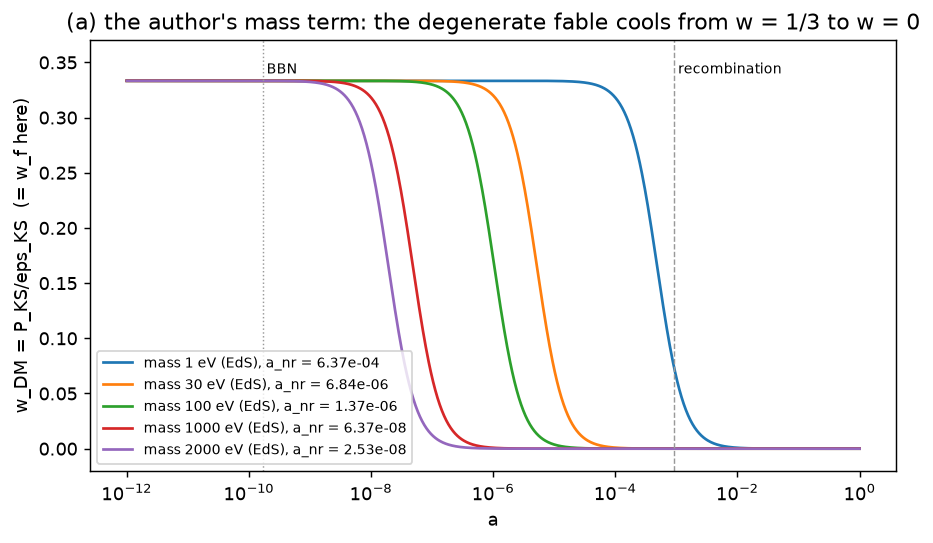
\includegraphics[width=0.75\linewidth]{nb06_a_mass_wdm.png}
  \caption{\texttt{fable-cosmology/\allowbreak results/\allowbreak nb06\_a\_mass\_wdm.png} (notebook 06, section 5.2), runs (a): the
  author's mass term, $\wDM=\PKS/\epsKS$ ($=w_f$ there) against $a$: the degenerate fable cools from $1/3$
  to 0.}
  \label{fig:nb06a}
\end{figure}

\subsection{Runs (b): a mass term plus a bare cosmological constant --- \texorpdfstring{$\Lambda$}{Lambda}CDM with fable dark matter}
\label{sec:9.5}

$W=V_0+m_0\sigma$, \texttt{fable4d}, $\Omegaqp=0.265$, $V_0$ (a bare Lambda) closing the budget \cfnb{nb06
\S5.3, figure \file{results/nb06_b_lambda_mass.png}} (figure~\ref{fig:nb06b}):

{\scriptsize
\setlength{\tabcolsep}{3pt}
\begin{center}
\begin{tabular}{@{}>{\raggedright\arraybackslash}p{0.3\linewidth}llllll@{}}
\toprule
run & $\anr$ & $\DNeff$ BBN & $\DNeff$ rec & $q_0$ & $t_0$ [Gyr] & $V_0=\rho_U$ \tabularnewline
\midrule
lambda-mass 30 eV & \texttt{4.4658e-06} & \texttt{0.07179} & \texttt{19.65} & \texttt{-0.52845} & \texttt{13.8000} & \texttt{0.685665} \tabularnewline
lambda-mass 100 eV & \texttt{8.9687e-07} & \texttt{0.01442} & \texttt{19.65} & \texttt{-0.52845} & \texttt{13.8000} & \texttt{0.685665} \tabularnewline
lambda-mass 1000 eV & \texttt{4.1629e-08} & \texttt{0.0006692} & \texttt{19.65} & \texttt{-0.52845} & \texttt{13.8000} & \texttt{0.685665} \tabularnewline
lambda-mass 2000 eV & \texttt{1.6521e-08} & \texttt{0.0002656} & \texttt{19.65} & \texttt{-0.52845} & \texttt{13.8000} & \texttt{0.685665} \tabularnewline
lambda-mass 30 eV (reference) & \texttt{4.4658e-06} & \texttt{0.07179} & \texttt{19.65} & \texttt{-0.52845} & \texttt{13.8000} & \texttt{0.685665} \tabularnewline
\bottomrule
\end{tabular}
\end{center}
}

\noindent and the observer's fits:

{\scriptsize
\setlength{\tabcolsep}{3pt}
\begin{center}
\begin{tabular}{@{}>{\raggedright\arraybackslash}p{0.28\linewidth}lll@{}}
\toprule
run & CPL $w_f$ $(w_0,w_a)$ & CPL $\wDE$ $(w_0,w_a)$ & $\max|\wDE+1|$, $a\geq0.3$ \tabularnewline
\midrule
lambda-mass 30 eV & \texttt{(-0.7573, +1.0100)} & \texttt{(-1.0000000003, +1.33e-09)} & \texttt{1.47e-09} \tabularnewline
lambda-mass 100 eV & \texttt{(-0.7573, +1.0100)} & \texttt{(-1.0000000000, +5.34e-11)} & \texttt{5.91e-11} \tabularnewline
lambda-mass 1000 eV & \texttt{(-0.7573, +1.0100)} & \texttt{(-1.0000000000, +1.16e-13)} & \texttt{1.31e-13} \tabularnewline
lambda-mass 2000 eV & \texttt{(-0.7573, +1.0100)} & \texttt{(-1.0000000000, +1.72e-14)} & \texttt{2.40e-14} \tabularnewline
lambda-mass 30 eV (reference) & \texttt{(-0.7569, +1.0092)} & \texttt{(-1.0000000003, +1.31e-09)} & \texttt{1.44e-09} \tabularnewline
\bottomrule
\end{tabular}
\end{center}
}

The mass does not vary ($\wDMeff=\wDM$, $Q=0$) and the condensate is the constant $V_0$, so the dark energy an
observer infers \textbf{is a cosmological constant}, to the precision of the quasiparticles' kinetic energy
that the observer counts as dark energy. The intrinsic $w_f$ today is \texttt{-0.72124767} [file:
\file{nb06_runs.csv}] --- it mixes the gas and $V_0$ and is not a dark-energy equation of state. The fifth run
($a_i=10^{-10}$, 701 rows, \file{results/nb06_fable4d_mass30eV.csv}) is Part~VIII's reference case
(\secref{sec:9.12}).

\begin{figure}[tbp]
  \centering
  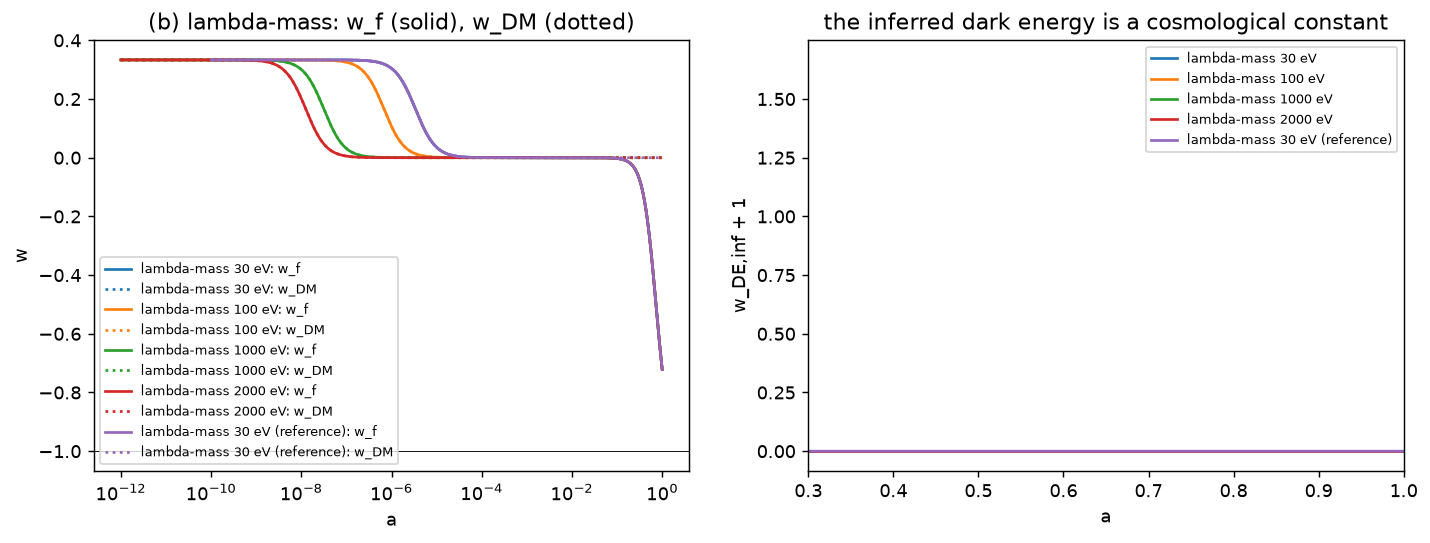
\includegraphics[width=0.95\linewidth]{nb06_b_lambda_mass.png}
  \caption{\texttt{fable-cosmology/\allowbreak results/\allowbreak nb06\_b\_lambda\_mass.png} (notebook 06, section 5.3), runs (b): $w_f$
  (solid) and $\wDM$ (dotted); and $\wDE+1$ on $0.3\leq a\leq1$: the inferred dark energy is a
  cosmological constant.}
  \label{fig:nb06b}
\end{figure}

\subsection{Runs (c): potentials with which the fable supplies the dark energy itself}
\label{sec:9.6}

\cfcode{power} ($\nu=0.236$, $0.5$), \cfcode{expdamp} (Part~VI's $x_t=1/2.21$), attractive \cfcode{quadratic}
($g_q=-0.5$), each at $\mtoday=30$ and $100$\,eV, \texttt{fable4d}, and Part~VIII's mass-varying reference case
(\cfcode{power}, $\nu=0.5$, $\mtoday=100$\,eV, $\Omegaqp=0.55$, 701 rows, \file{results/nb06_fable4d_power.csv})
\cfnb{nb06 \S5.4, figures \file{results/nb06_c_de_potentials.png},
\file{results/nb06_c_exchange_vacuum_stabilizer.png}} (figures~\ref{fig:nb06c1} and~\ref{fig:nb06c2}):

{\scriptsize
\setlength{\tabcolsep}{3pt}
\begin{center}
\begin{tabular}{@{}>{\raggedright\arraybackslash}p{0.25\linewidth}llllll@{}}
\toprule
run & $\anr$ & \parbox[t]{2.0cm}{\raggedright min $m/\mtoday$ ($10^{-3}\leq a\leq0.3$)} & $w_f(1)$ & min $w_f$ & CPL $w_f$ & min $c_s^2$ \tabularnewline
\midrule
power nu=0.236, 30 eV & \texttt{2.22e-05} & \texttt{2.01e-01} & \texttt{-0.7212} & \texttt{-0.7212} & \texttt{(-0.783, +0.445)} & \texttt{-0.611} \tabularnewline
power nu=0.236, 100 eV & \texttt{4.47e-06} & \texttt{2.01e-01} & \texttt{-0.7212} & \texttt{-0.7212} & \texttt{(-0.783, +0.445)} & \texttt{-0.611} \tabularnewline
power nu=0.5, 30 eV & \texttt{0.669} & \texttt{7.91e-12} & \texttt{-0.7212} & \texttt{-1.0000} & \texttt{(-0.804, -0.358)} & \texttt{-27} \tabularnewline
power nu=0.5, 100 eV & \texttt{0.669} & \texttt{1.59e-12} & \texttt{-0.7212} & \texttt{-1.0000} & \texttt{(-0.804, -0.359)} & \texttt{-27} \tabularnewline
expdamp xt=1/2.21, 30 eV & \texttt{0.712} & \texttt{6.58e-12} & \texttt{-0.7212} & \texttt{-1.0000} & \texttt{(-0.829, -0.317)} & \texttt{-21.8} \tabularnewline
expdamp xt=1/2.21, 100 eV & \texttt{0.712} & \texttt{1.32e-12} & \texttt{-0.7212} & \texttt{-1.0000} & \texttt{(-0.829, -0.317)} & \texttt{-21.8} \tabularnewline
quadratic gq=$-$0.5, 30 eV & \texttt{0.643} & \texttt{8.93e-12} & \texttt{-0.7212} & \texttt{-1.0000} & \texttt{(-0.730, -0.483)} & \texttt{-47.1} \tabularnewline
quadratic gq=$-$0.5, 100 eV & \texttt{0.643} & \texttt{1.79e-12} & \texttt{-0.7212} & \texttt{-1.0000} & \texttt{(-0.730, -0.483)} & \texttt{-47.1} \tabularnewline
power nu=0.5, 100 eV, $\Omegaqp=0.55$ & \texttt{4.21e-06} & \texttt{2.72e-01} & \texttt{-0.4215} & \texttt{-0.4215} & \texttt{(-0.448, +0.264)} & \texttt{-0.364} \tabularnewline
\bottomrule
\end{tabular}
\end{center}
}

\noindent and the observer's inferred dark energy:

{\scriptsize
\setlength{\tabcolsep}{3pt}
\begin{center}
\begin{tabular}{@{}>{\raggedright\arraybackslash}p{0.25\linewidth}lllll@{}}
\toprule
run & poles of $\wDE$ & $w=-1$ crossings & \parbox[t]{1.9cm}{\raggedright phantom in $0.3\leq a\leq1$?} & CPL $\wDE$ & fit from $a$ \tabularnewline
\midrule
power nu=0.236, 30 eV & \texttt{3.43e-06, 0.533} & \texttt{4.55966e-06, 1} & True & \texttt{(-0.082, -7.986)} & \texttt{0.559} \tabularnewline
power nu=0.236, 100 eV & \texttt{6.89e-07, 0.533} & \texttt{9.15884e-07, 1} & True & \texttt{(-0.082, -7.986)} & \texttt{0.559} \tabularnewline
power nu=0.5, 30 eV & \texttt{3.35e-06, 0.619} & \texttt{4.46748e-06, 1} & True & \texttt{(-0.249, -10.191)} & \texttt{0.650} \tabularnewline
power nu=0.5, 100 eV & \texttt{6.73e-07, 0.619} & \texttt{8.97015e-07, 1} & True & \texttt{(-0.249, -10.191)} & \texttt{0.650} \tabularnewline
expdamp xt=1/2.21, 30 eV & \texttt{3.35e-06, 0.625} & \texttt{4.46748e-06, 1} & True & \texttt{(-0.128, -11.778)} & \texttt{0.656} \tabularnewline
expdamp xt=1/2.21, 100 eV & \texttt{6.73e-07, 0.625} & \texttt{8.97015e-07, 1} & True & \texttt{(-0.128, -11.779)} & \texttt{0.656} \tabularnewline
quadratic gq=$-$0.5, 30 eV & \texttt{3.35e-06, 0.602} & \texttt{4.46748e-06, 1} & True & \texttt{(-0.180, -9.321)} & \texttt{0.632} \tabularnewline
quadratic gq=$-$0.5, 100 eV & \texttt{6.73e-07, 0.602} & \texttt{8.97015e-07, 1} & True & \texttt{(-0.180, -9.321)} & \texttt{0.632} \tabularnewline
power nu=0.5, 100 eV, $\Omegaqp=0.55$ & \texttt{8.96e-07, 0.63} & \texttt{1.18957e-06, 1} & True & \texttt{(-0.327, -9.682)} & \texttt{0.662} \tabularnewline
\bottomrule
\end{tabular}
\end{center}
}

\noindent and, for the same runs \cfnb{nb06 \S5.4}:

{\scriptsize
\setlength{\tabcolsep}{3pt}
\begin{center}
\begin{tabular}{@{}>{\raggedright\arraybackslash}p{0.23\linewidth}lllll@{}}
\toprule
run & \parbox[t]{1.6cm}{\raggedright $c_s^2<0$ on\ ($a\geq10^{-3}$)} & \parbox[t]{2.2cm}{\raggedright $\wDMeff$ range\ ($a\geq10^{-3}$)} & \parbox[t]{1.7cm}{\raggedright $|\Evac|/\rho_{\mathrm{tot}}$,\ $a\geq0.3$} & $\Pstab(1)$ [$\rhoc$] & $\DNeff$ BBN \tabularnewline
\midrule
power nu=0.236, 30 eV & \texttt{[0.00409, 1]} & \texttt{(-0.611, +9.85e-05)} & \texttt{1.314e+13} & \texttt{-0.8428} & \texttt{0.0718} \tabularnewline
power nu=0.236, 100 eV & \texttt{[0.00194, 1]} & \texttt{(-0.611, +3.59e-06)} & \texttt{1.622e+15} & \texttt{-0.8428} & \texttt{0.0144} \tabularnewline
power nu=0.5, 30 eV & \texttt{[0.608, 1]} & \texttt{(-27.6, +0.333)} & \texttt{2.229e+14} & \texttt{-0.8428} & \texttt{0.0718} \tabularnewline
power nu=0.5, 100 eV & \texttt{[0.608, 1]} & \texttt{(-27.7, +0.333)} & \texttt{2.752e+16} & \texttt{-0.8428} & \texttt{0.0144} \tabularnewline
expdamp xt=1/2.21, 30 eV & \texttt{[0.643, 1]} & \texttt{(-21.8, +0.333)} & \texttt{2.327e+14} & \texttt{-0.8428} & \texttt{0.0718} \tabularnewline
expdamp xt=1/2.21, 100 eV & \texttt{[0.643, 1]} & \texttt{(-21.8, +0.333)} & \texttt{2.873e+16} & \texttt{-0.8428} & \texttt{0.0144} \tabularnewline
quadratic gq=$-$0.5, 30 eV & \texttt{[0.592, 1]} & \texttt{(-47.1, +0.333)} & \texttt{2.031e+14} & \texttt{-0.8428} & \texttt{0.0718} \tabularnewline
quadratic gq=$-$0.5, 100 eV & \texttt{[0.592, 1]} & \texttt{(-47.1, +0.333)} & \texttt{2.508e+16} & \texttt{-0.8428} & \texttt{0.0144} \tabularnewline
power nu=0.5, 100 eV, $\Omegaqp=0.55$ & \texttt{[0.001, 1]} & \texttt{(-0.364, -3.89e-05)} & \texttt{2.350e+14} & \texttt{-0.7003} & \texttt{0.0382} \tabularnewline
\bottomrule
\end{tabular}
\end{center}
}

\noindent and
\cfcode{smallest w_f over all 9 runs: -0.9999987921 (never below -1);  every run has c_s^2 < 0 somewhere after a = 1e-3: True}.
Reading the tables:
\begin{itemize}
  \item Only the two $\nu=0.236$ runs and the reference run stay \textbf{massive} through the matter era. The
        $\nu=0.5$, \cfcode{expdamp} and \cfcode{quadratic} runs with $\Omegaqp=0.265$ have
        $\min m/\mtoday\sim10^{-12}$: the gap pins their mass near zero and the fable is a \textbf{massless
        gas} (radiation, $w=1/3$) until $\anr=0.64$--$0.71$ --- it supplies no dark matter at recombination
        ($\DNeff$ at recombination equals its BBN value, e.g.\ \texttt{0.071792425} for
        \cfcode{power nu=0.5, 30 eV} [file: \file{nb06_runs.csv}]). Their CPL fits of $w_f$ look like the
        supernova fits $(-0.861,-0.60)$, but they are not viable cosmologies.
  \item The observer's inferred dark energy $\wDE$ has \textbf{poles} (its $\rhoDE$ changes sign) inside
        $0.3\leq a\leq1$ in every run, and it is phantom and crosses $-1$ in every run; a CPL line is not a
        faithful description (the fits above the pole are in \file{results/nb06_cpl_fits.csv}).
  \item $c_s^2<0$ in every run: an \textbf{adiabatic instability}.
  \item The Dirac-sea energy that the no-sea functional drops changes along every run by
        $1.31\times10^{13}$ to $2.87\times10^{16}$ times the total density at $a\geq0.3$.
\end{itemize}

\begin{figure}[tbp]
  \centering
  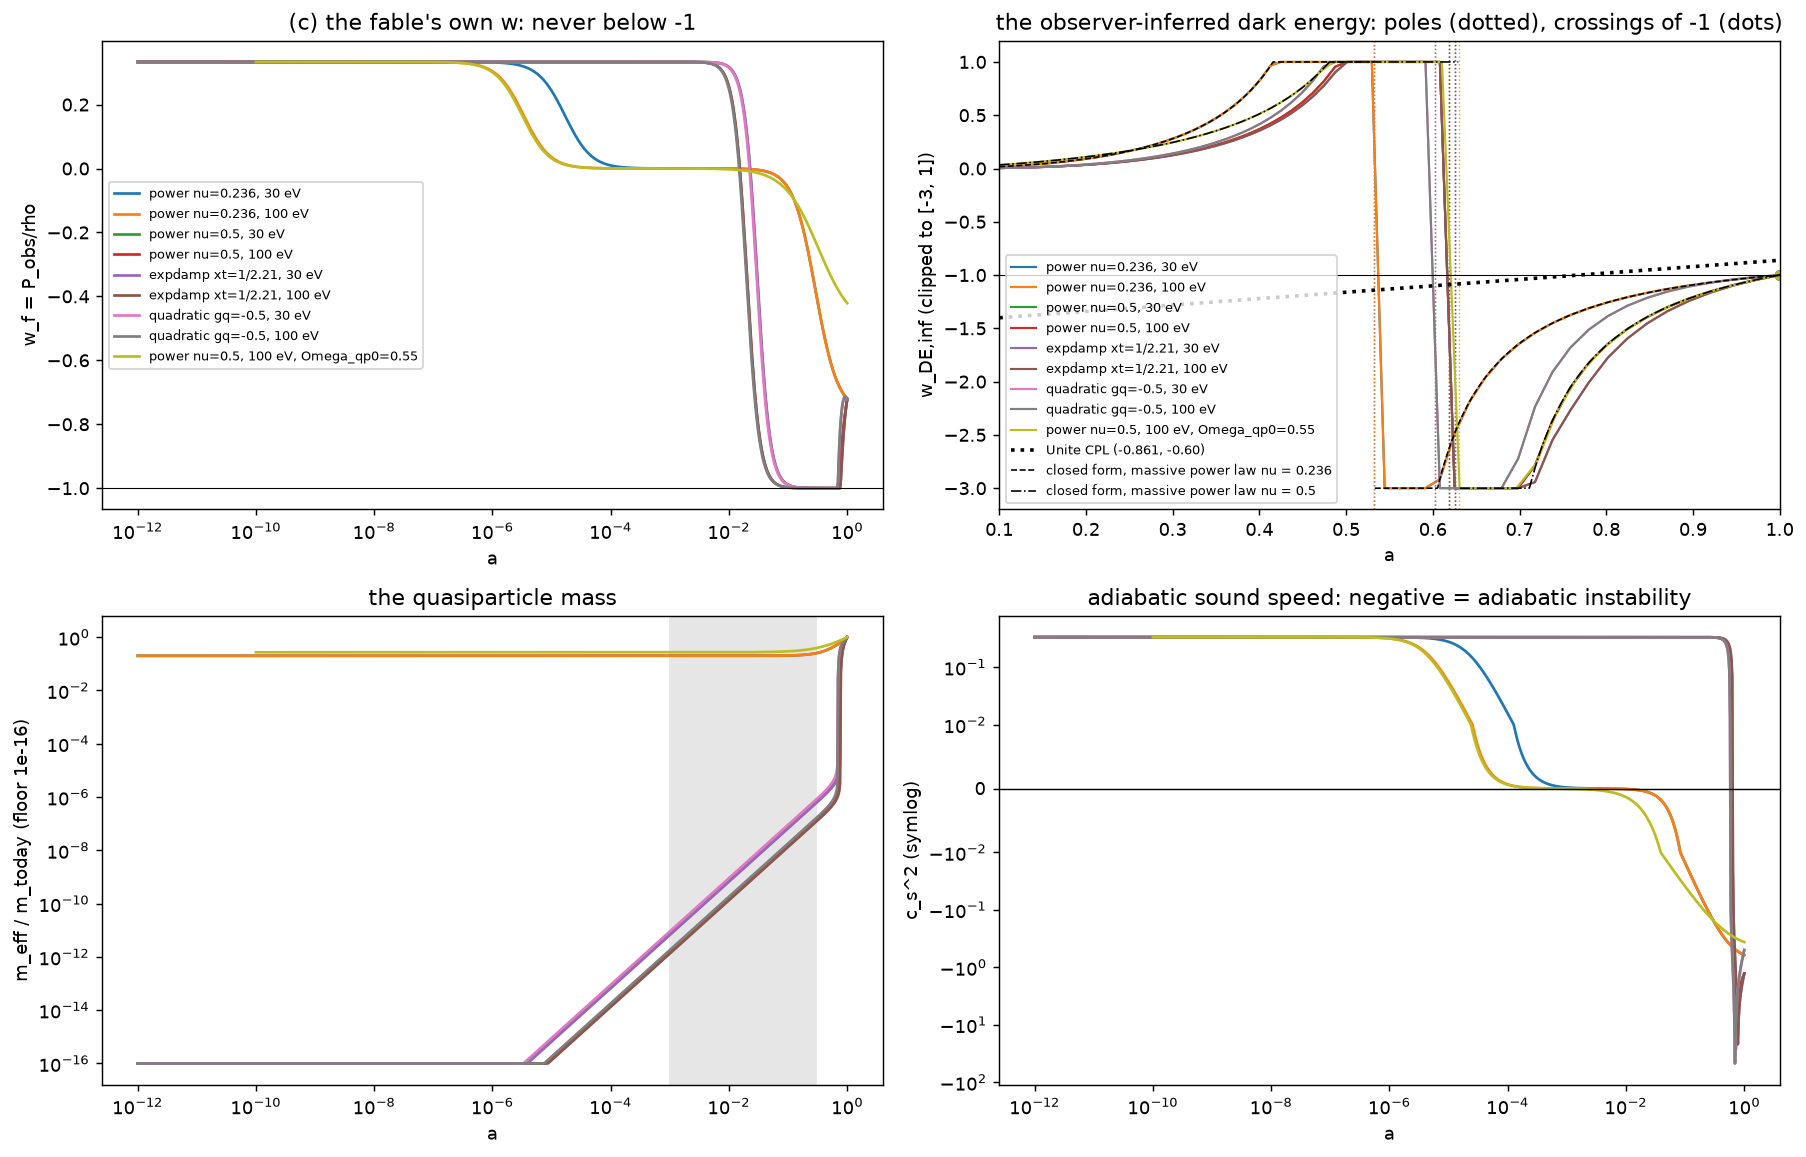
\includegraphics[width=0.95\linewidth]{nb06_c_de_potentials.png}
  \caption{\texttt{fable-cosmology/\allowbreak results/\allowbreak nb06\_c\_de\_potentials.png} (notebook 06, section 5.4), runs (c):
  $w_f$ (never below $-1$), the observer's $\wDE$ (clipped to $[-3,1]$, poles and crossings marked),
  $\meffx/\mtoday$, and $c_s^2$ (negative below the line).}
  \label{fig:nb06c1}
\end{figure}
\begin{figure}[tbp]
  \centering
  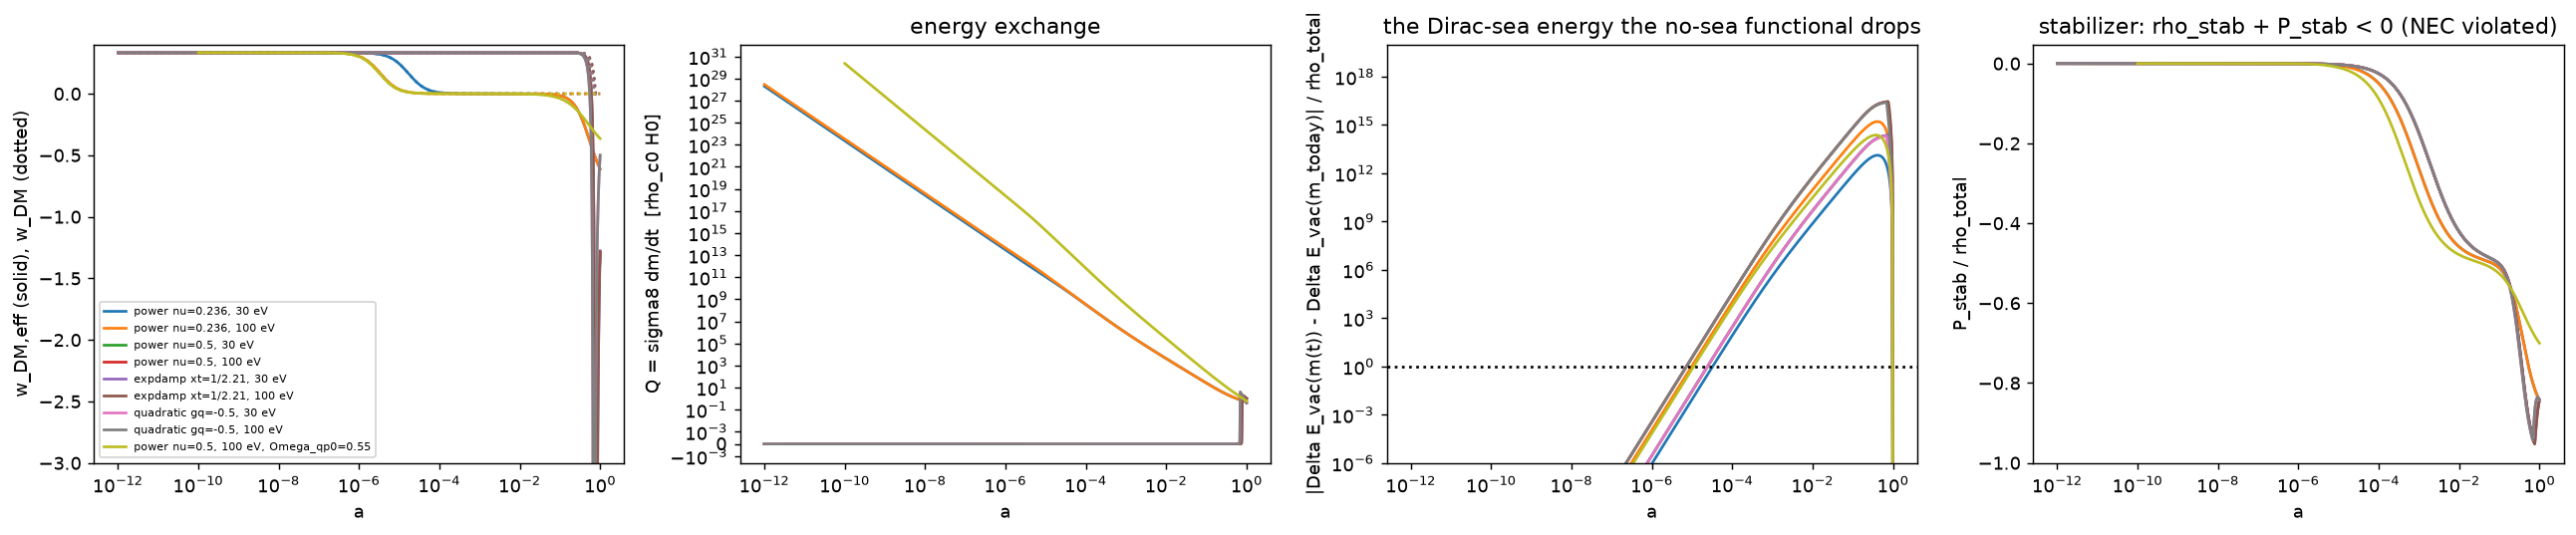
\includegraphics[width=\linewidth]{nb06_c_exchange_vacuum_stabilizer.png}
  \caption{\texttt{fable-cosmology/\allowbreak results/\allowbreak nb06\_c\_exchange\_vacuum\_stabilizer.png} (notebook 06, section 5.4),
  runs (c): $\wDM$ and $\wDMeff$, the exchange $Q$, the Dirac-sea energy relative to the total density, and
  $\Pstab/\rho$.}
  \label{fig:nb06c2}
\end{figure}

\subsection{The inferred dark energy of a massive power law, in closed form}
\label{sec:9.7}

Once the gas is non-relativistic, $\sigma_8\approx n\propto a^{-3}$, the condensate is $U=U_t\,a^{-3\nu}$ and the
mass $m(a)=m_0+\nu\,U_t\,a^{3(1-\nu)}/\bigl((1-\nu)\,\sigma_t\bigr)$. Subtracting cold dark matter with today's
mass leaves $\rhoDE=U+\bigl(m(a)-\mtoday\bigr)\,n=U_t\bigl[a^{-3\nu}-\nu\,a^{-3}\bigr]/(1-\nu)$ and $P_{\mathrm{DE}}=-U$,
hence
\[
  \wDE(a)=-\frac{1-\nu}{1-\nu\,a^{-3(1-\nu)}} ,
\]
a pole at $a_{\mathrm{pole}}=\nu^{1/(3(1-\nu))}$, $w>0$ before it, phantom ($w<-1$) between it and today, and
$w=-1$ at $a=1$ up to the quasiparticles' kinetic energy, which makes it cross $-1$ just before today. It
depends on $\nu$ alone [prose nb06 \S5.4]. The runs agree \cfnb{nb06 \S5.4}:
\begin{Verbatim}[fontsize=\scriptsize]
power nu=0.236, 30 eV                  w_DE,inf against -(1-nu)/(1 - nu a^(-3(1-nu))) on a >= 0.3: max deviation 1.2e-09;  pole: formula 0.532600, run 0.532723;  crossing of -1: 1.00000000
power nu=0.236, 100 eV                 w_DE,inf against -(1-nu)/(1 - nu a^(-3(1-nu))) on a >= 0.3: max deviation 4.9e-11;  pole: formula 0.532600, run 0.532723;  crossing of -1: 1.00000000
power nu=0.5, 100 eV, Omega_qp0=0.55   w_DE,inf against -(1-nu)/(1 - nu a^(-3(1-nu))) on a >= 0.3: max deviation 4.2e-11;  pole: formula 0.629961, run 0.630028;  crossing of -1: 1.00000000
\end{Verbatim}
The mechanism is that of Das, Corasaniti and Khoury, Phys.\ Rev.\ D \textbf{73}, 083509 (2006): subtracting
cold dark matter with today's mass when the mass was different leaves
$\rho_{\mathrm{DE}}+P_{\mathrm{DE}}\approx\bigl(\meffx(a)-\mtoday\bigr)\,n$, which is negative whenever $\meffx$
grows; an apparent phantom with no phantom field.

\subsection{The scans: where does a dark-energy fable stay massive through the matter era?}
\label{sec:9.8}

Notebook 06 scanned the shape parameters --- \cfcode{power} $\nu=0.05\dots0.65$, \cfcode{quadratic}
$g_q=-0.95\dots-0.05$, \cfcode{expdamp} $x_t=0.1\dots0.9$, and for \cfcode{power} $\nu=0.3$ and $0.5$ the
quasiparticle share $\Omegaqp=0.265\dots0.8$ --- at $\mtoday=1000$\,eV and $100$\,eV (\texttt{fable4d}, 401
output rows, $45+45$ runs), and re-computed every scan run independently as it ran \cfnb{nb06 \S5.6, files
\file{results/nb06_scan.csv}, figures \file{results/nb06_scan.png}, \file{results/nb06_scan_cpl.png}}
(figures~\ref{fig:nb06scan} and~\ref{fig:nb06scancpl}). Its conclusions, verbatim:
\begin{Verbatim}[fontsize=\scriptsize]
scan points whose fable stays massive through 1e-3 <= a <= 0.3 (min m/m_today > 1e-3): 28 of 90: power, nu=0.05 (1000 eV), power, nu=0.1 (1000 eV), power, nu=0.15 (1000 eV), power, nu=0.2 (1000 eV), power, nu=0.25 (1000 eV), power nu=0.3, Omega_qp0=0.35 (1000 eV), power nu=0.3, Omega_qp0=0.45 (1000 eV), power nu=0.3, Omega_qp0=0.55 (1000 eV), power nu=0.3, Omega_qp0=0.65 (1000 eV), power nu=0.3, Omega_qp0=0.8 (1000 eV), power nu=0.5, Omega_qp0=0.5 (1000 eV), power nu=0.5, Omega_qp0=0.55 (1000 eV), power nu=0.5, Omega_qp0=0.65 (1000 eV), power nu=0.5, Omega_qp0=0.8 (1000 eV), power, nu=0.05 (100 eV), power, nu=0.1 (100 eV), power, nu=0.15 (100 eV), power, nu=0.2 (100 eV), power, nu=0.25 (100 eV), power nu=0.3, Omega_qp0=0.35 (100 eV), power nu=0.3, Omega_qp0=0.45 (100 eV), power nu=0.3, Omega_qp0=0.55 (100 eV), power nu=0.3, Omega_qp0=0.65 (100 eV), power nu=0.3, Omega_qp0=0.8 (100 eV), power nu=0.5, Omega_qp0=0.5 (100 eV), power nu=0.5, Omega_qp0=0.55 (100 eV), power nu=0.5, Omega_qp0=0.65 (100 eV), power nu=0.5, Omega_qp0=0.8 (100 eV)
of these, with c_s^2 >= 0 after a = 1e-3: 0;  smallest c_s^2 among them: -0.6469;  largest: -0.0565
power law: 'massive through the matter era' <=> 'bare m0 > 0' at all 52 power scan points: True
the estimate Omega_qp0/U_t > nu/(1 - nu) agrees with the sign of m0 at 52 of 52 points;  with Omega_qp0 = 0.265 it allows nu < Omega_qp0/(1 - Omega_b0 - Omega_r0) = 0.2788
\end{Verbatim}
So: \textbf{every \cfcode{quadratic} and \cfcode{expdamp} point is massless in the matter era; a power law
stays massive exactly when its bare mass $m_0=\mtoday-\nu\lambda\sigma_t^{\nu-1}$ is positive, i.e.\ when
$\Omegaqp/U_t>\nu/(1-\nu)$; with the observed split $\Omegaqp=0.265$ that requires $\nu<0.2788$} (massive up to
$\nu=0.25$, massless from $\nu=0.3$ in the scan); a larger $\nu$ needs a larger quasiparticle share
($\Omegaqp\geq0.35$ for $\nu=0.3$, $\geq0.5$ for $\nu=0.5$). And every massive point has $c_s^2<0$ after
$a=10^{-3}$. (At high density $\nu\lambda\sigma^{\nu-1}\to0$, so if $m_0<0$ the gap can only be met with $m\to0^+$;
with $\sigma_t\approx n_t$ and $\epsKS\approx\mtoday\,n_t$ today this happens exactly when
$\Omegaqp/U_t<\nu/(1-\nu)$ [prose nb06 \S5.6].) In the massless cases the smallest $c_s^2$ sits at the sharp
release of the pinned gap, and its magnitude depends on how finely the output grid samples that release; its
sign does not [prose nb06 \S5.6]. The largest cross-check difference over the 90 scan runs is
\texttt{4.43e-09} \cfnb{nb06 \S5.10}.

\begin{figure}[tbp]
  \centering
  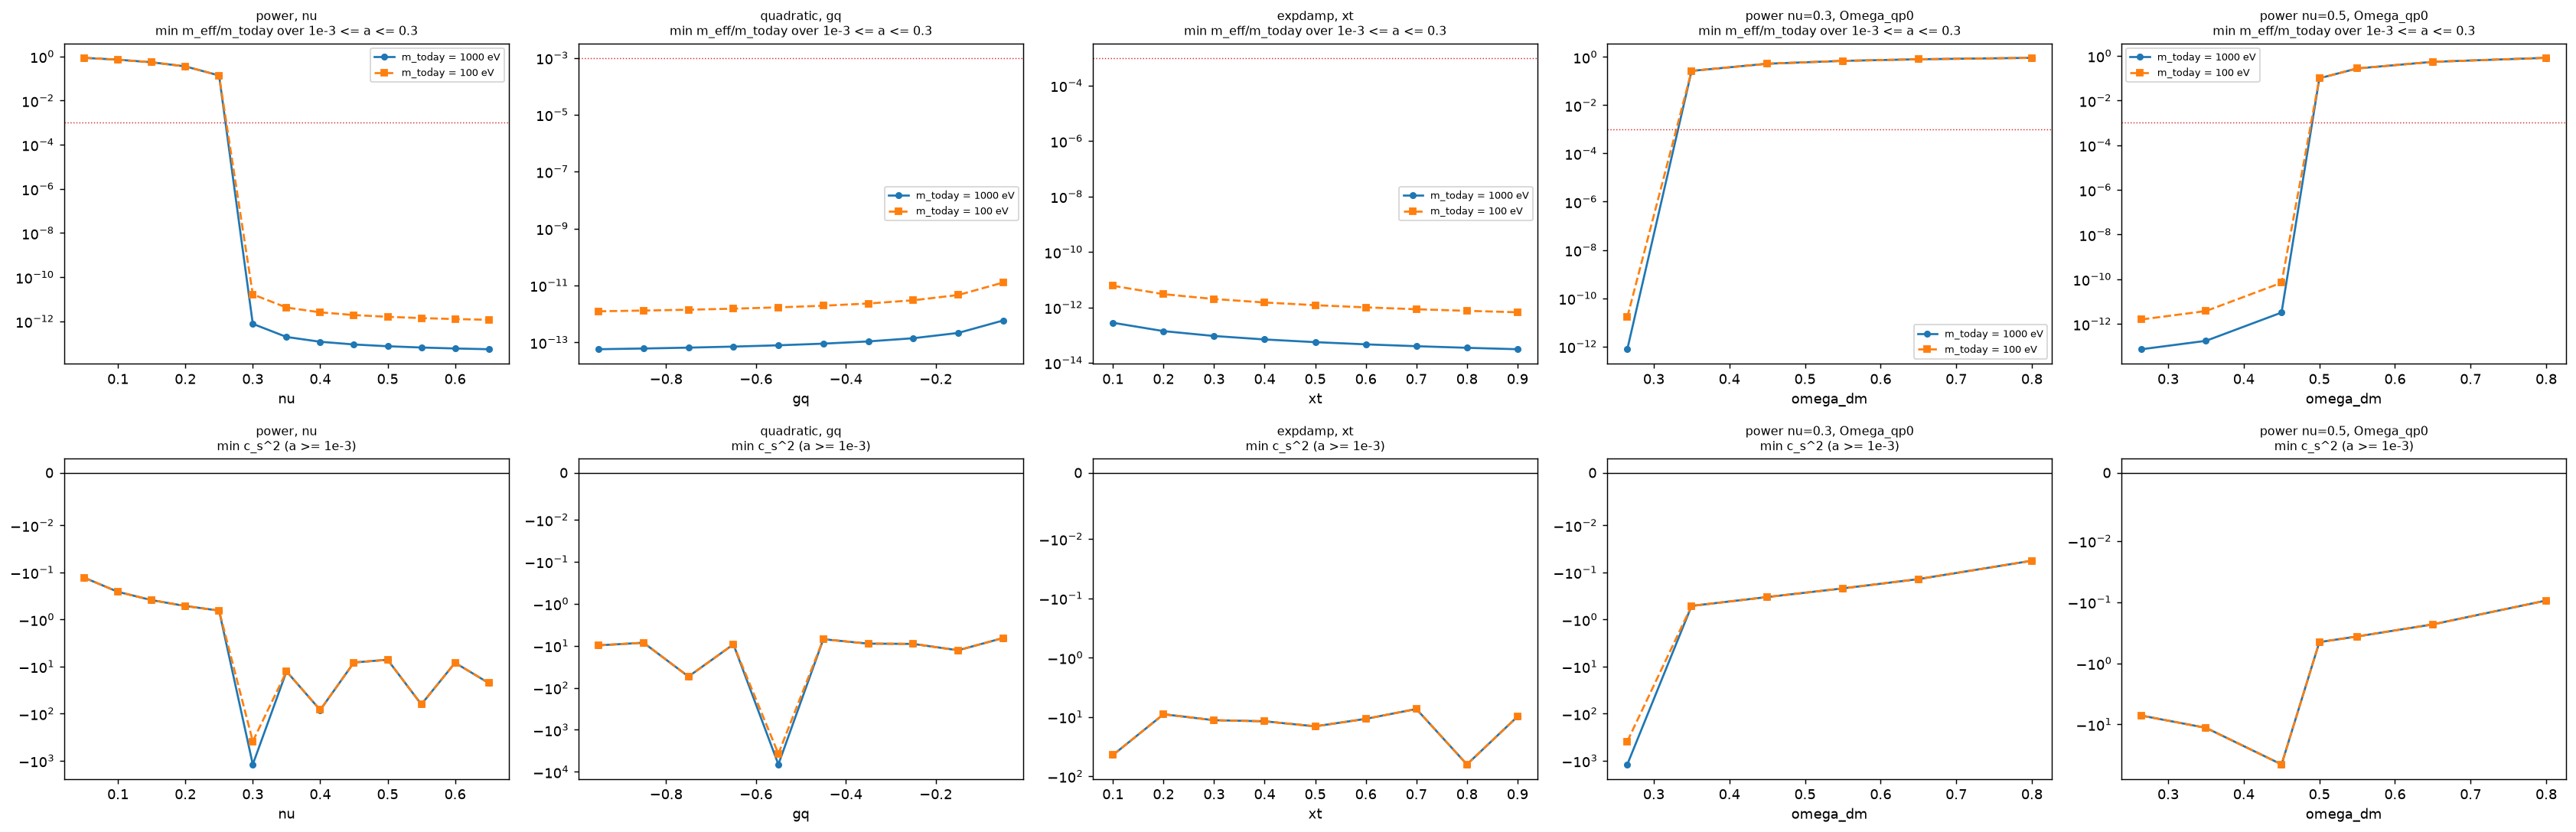
\includegraphics[width=\linewidth]{nb06_scan.png}
  \caption{\texttt{fable-cosmology/\allowbreak results/\allowbreak nb06\_scan.png} (notebook 06, section 5.6), the scans: per family, the
  smallest $\meffx/\mtoday$ over $10^{-3}\leq a\leq0.3$ and the smallest $c_s^2$ ($a\geq10^{-3}$) against the
  scanned parameter.}
  \label{fig:nb06scan}
\end{figure}
\begin{figure}[tbp]
  \centering
  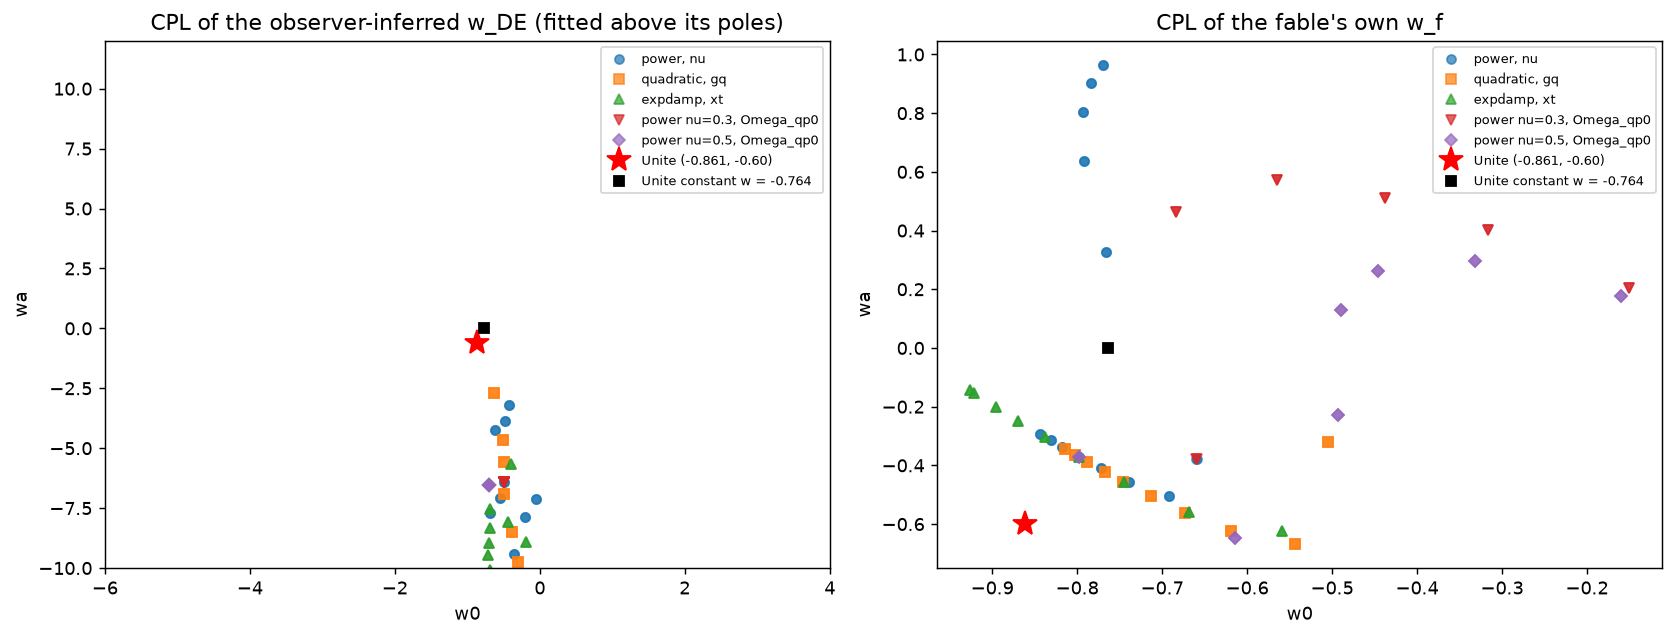
\includegraphics[width=0.95\linewidth]{nb06_scan_cpl.png}
  \caption{\texttt{fable-cosmology/\allowbreak results/\allowbreak nb06\_scan\_cpl.png} (notebook 06, section 5.6), the scans: the CPL
  points $(w_0,w_a)$ of $\wDE$ (fitted above its poles) and of $w_f$.}
  \label{fig:nb06scancpl}
\end{figure}

\subsection{How heavy must a fable that is all of the dark matter be?}
\label{sec:9.9}

\cfnb{nb06 \S5.7, file \file{results/nb06_dm_mass_bounds.csv}, figure \file{results/nb06_dm_mass_bounds.png}}
(figure~\ref{fig:nb06dm})

{\small
\renewcommand{\arraystretch}{1.3}
\begin{center}
\begin{tabular}{@{}>{\raggedright\arraybackslash}p{0.36\linewidth}>{\raggedright\arraybackslash}p{0.17\linewidth}>{\raggedright\arraybackslash}p{0.41\linewidth}@{}}
\toprule
bound & fable mass & detail \tabularnewline
\midrule
$\DNeff(\mathrm{BBN})<0.3$ & $m>10.2645$\,eV & fit over 17 runs: $\DNeff=6.6922\,(m/\mathrm{eV})^{-1.33333}$, max $|\ln\text{residual}|=$ \texttt{7.1e-05} \tabularnewline
$\DNeff(\mathrm{BBN})<0.2$ & $m>13.9126$\,eV & same fit \tabularnewline
free streaming: $v_{\mathrm{rms}0}$ matched to thermal WDM of 3.3\,keV (Viel et al.\ 2013) & $m\approx1124.92$\,eV & $v_{\mathrm{rms}0}=$ \texttt{8.2629e-03} km/s \tabularnewline
free streaming: $v_{\mathrm{rms}0}$ matched to thermal WDM of 5.3\,keV (Ir\v{s}i\v{c} et al.\ 2017) & $m\approx1806.69$\,eV & $v_{\mathrm{rms}0}=$ \texttt{4.3932e-03} km/s \tabularnewline
Tremaine--Gunn, $g=8$, $\sigma=10$\,km/s, $r_c=0.3$\,kpc & $m>231.315$\,eV & $m^4>9\,h^3/\bigl(2\,(2\pi)^{5/2}\,g\,G\,\sigma\,r_c^2\bigr)$ \tabularnewline
Tremaine--Gunn, $g=8$, $\sigma=7$\,km/s, $r_c=0.15$\,kpc & $m>357.639$\,eV & same \tabularnewline
\bottomrule
\end{tabular}
\end{center}
}

\noindent$\DNeff\propto m^{-4/3}$ because $\DNeff(\mathrm{BBN})$ depends only on $k_{F0}$, which
$\epsKS(m,k_{F0})=\Omegaqp$ fixes, and $k_{F0}\propto m^{-1/3}$ for a non-relativistic gas today; at 1, 30, 100,
1000, 2000\,eV it is \texttt{6.69227}, \texttt{0.0717924}, \texttt{0.0144181}, \texttt{0.000669238},
\texttt{0.00026561}. A degenerate gas has the velocity dispersion of a filled Fermi sphere,
$v_{\mathrm{rms}}=\sqrt{3/5}\,\kF/m$: \texttt{4.4870e+00}, \texttt{2.6132e+00}, \texttt{2.0827e-01},
\texttt{9.6670e-03}, \texttt{3.8364e-03} km/s at 10, 15, 100, 1000, 2000\,eV. The Lyman-alpha-allowed
thermal-relic warm dark matter ($m_{\mathrm{WDM}}\gtrsim3.3$\,keV and 5.3\,keV) has $v_{\mathrm{rms}0}=$
\texttt{8.2629e-03} and \texttt{4.3932e-03} km/s; a degenerate fable with the same $v_{\mathrm{rms}0}$ needs
$m\approx1.1$--$1.8$\,keV --- a velocity-matching estimate, not a transfer-function computation. The
Tremaine--Gunn bound uses illustrative dwarf-spheroidal values (inputs, not results). The free-streaming
bound is far stronger than $\DNeff$. At such masses the change of $\wDM$ from $1/3$ to 0 happens around
$\anr=4.16\times10^{-8}$ (1\,keV) or $1.65\times10^{-8}$ (2\,keV).

\begin{figure}[tbp]
  \centering
  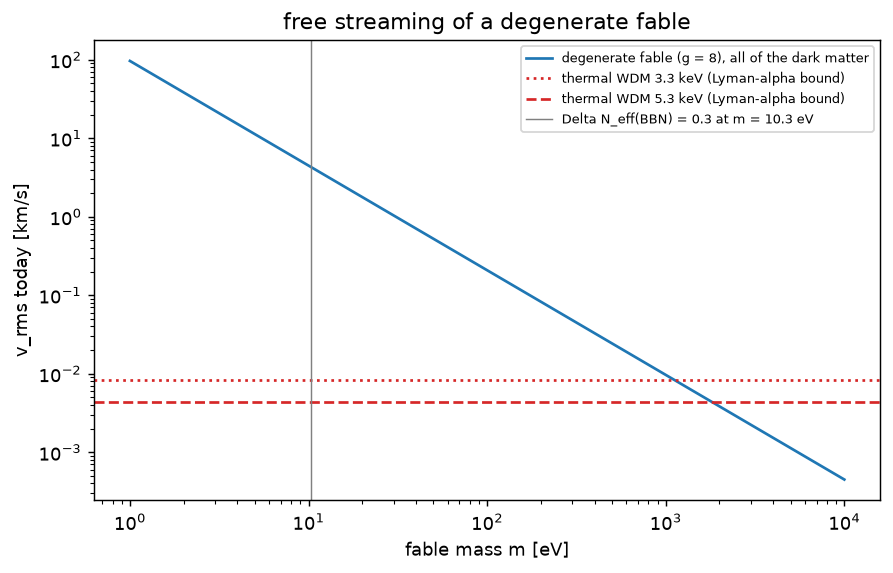
\includegraphics[width=0.75\linewidth]{nb06_dm_mass_bounds.png}
  \caption{\texttt{fable-cosmology/\allowbreak results/\allowbreak nb06\_dm\_mass\_bounds.png} (notebook 06, section 5.7): the free
  streaming of a degenerate fable: $v_{\mathrm{rms}}$ today against the fable mass, with the warm-dark-matter
  velocities.}
  \label{fig:nb06dm}
\end{figure}

\subsection{Runs (d): without the stabilizer, the hidden sheet moves and the Newton constant varies}
\label{sec:9.10}

\texttt{fable8d} for the mass term at 1 and 100\,eV and \cfcode{lambda-mass} at 30\,eV and 1\,keV, and two
controls: radiation alone (\cfcode{--no-fable --omega-b 0}), which must keep the hidden sheet exactly frozen
($F=0$), and radiation plus baryons (\cfcode{--no-fable}), in which dust alone drives it.
$G(a)/G(1)=1/v$ (the observed Newton constant is $G_4=G_8/\Vhidx\propto1/v$) \cfnb{nb06 \S5.8, file
\file{results/nb06_nogo_8d.csv}, figure \file{results/nb06_d_nogo_8d.png}} (figure~\ref{fig:nb06d}):

{\scriptsize
\setlength{\tabcolsep}{3pt}
\begin{center}
\begin{tabular}{@{}>{\raggedright\arraybackslash}p{0.24\linewidth}lllll@{}}
\toprule
run & $B(a_i)=C(a_i)$ & $G(a_i)/G(1)$ & $G(\mathrm{BBN})/G(1)$ & $\Delta G/G$ since BBN & $|d\ln G/dt|$ today [/yr] \tabularnewline
\midrule
mass 1 eV, fable8d & \texttt{2.3224e-03} & \texttt{3.4376e+10} & \texttt{3.4376e+10} & \texttt{-1.0000e+00} & \texttt{2.7571e-10} \tabularnewline
mass 100 eV, fable8d & \texttt{4.8207e-05} & \texttt{1.8516e+17} & \texttt{1.8516e+17} & \texttt{-1.0000e+00} & \texttt{2.7571e-10} \tabularnewline
lambda-mass 30 eV, fable8d & \texttt{9.8881e-04} & \texttt{1.0461e+12} & \texttt{1.0461e+12} & \texttt{-1.0000e+00} & \texttt{2.7570e-10} \tabularnewline
lambda-mass 1 keV, fable8d & \texttt{9.8389e-04} & \texttt{1.0671e+12} & \texttt{1.0671e+12} & \texttt{-1.0000e+00} & \texttt{2.7570e-10} \tabularnewline
radiation only, fable8d & \texttt{1.0000e+00} & \texttt{1.0000e+00} & \texttt{1.0000e+00} & \texttt{0.0000e+00} & \texttt{0.0000e+00} \tabularnewline
radiation + baryons, fable8d & \texttt{6.2532e-03} & \texttt{6.5402e+08} & \texttt{6.5402e+08} & \texttt{-1.0000e+00} & \texttt{2.3096e-11} \tabularnewline
\bottomrule
\end{tabular}
\end{center}
}

\noindent and the state of the hidden sheet and of the observer today:

{\scriptsize
\setlength{\tabcolsep}{3pt}
\begin{center}
\begin{tabular}{@{}>{\raggedright\arraybackslash}p{0.24\linewidth}lllll@{}}
\toprule
run & $H_B/H_A(1)={}$ $H_C/H_A(1)$ & max constraint residual & $\Omega_{\mathrm{sum}}(1)$ & $q_0$ & $t_0$ [Gyr] \tabularnewline
\midrule
mass 1 eV, fable8d & \texttt{0.999959} & \texttt{1.16e-08} & \texttt{6.99967} & \texttt{2.5000} & \texttt{4.145} \tabularnewline
mass 100 eV, fable8d & \texttt{0.999963} & \texttt{2.12e-08} & \texttt{6.99971} & \texttt{2.5000} & \texttt{4.145} \tabularnewline
lambda-mass 30 eV, fable8d & \texttt{0.999902} & \texttt{2.47e-08} & \texttt{6.99922} & \texttt{-0.8425} & \texttt{9.472} \tabularnewline
lambda-mass 1 keV, fable8d & \texttt{0.999902} & \texttt{2.07e-08} & \texttt{6.99922} & \texttt{-0.8425} & \texttt{9.472} \tabularnewline
radiation only, fable8d & \texttt{0.000000} & \texttt{9.89e-16} & \texttt{1.00000} & \texttt{1.0000} & \texttt{755.851} \tabularnewline
radiation + baryons, fable8d & \texttt{0.994782} & \texttt{1.04e-08} & \texttt{6.95831} & \texttt{2.4935} & \texttt{49.354} \tabularnewline
\bottomrule
\end{tabular}
\end{center}
}

Radiation alone keeps $H_B=H_C=0$ exactly (\cfcode{max |H_B/H_A| = 0.0e+00}: $F=0$); dust or vacuum energy drives
the hidden sheet to the 7-dimensional isotropic attractor ($H_B/H_A\to1$), and the observed Newton constant
changes by $\boldsymbol{6.5\times10^{8}}$ \textbf{to} $\boldsymbol{1.9\times10^{17}}$ between the start and
today, with $|d\ln G/dt|$ today $2.3\times10^{-11}$ to $2.76\times10^{-10}$\,/yr against the lunar-laser-ranging
bound $10^{-13}$\,/yr, and $\Delta G/G$ since nucleosynthesis $-1$ against the bound of about $0.1$. The closure
today then needs $\Omega_{\mathrm{sum}}(1)\approx7$
($\sum\Omega_i=1+\bigl(3H_B^2+9H_AH_B+3H_AH_C+3H_BH_C\bigr)/(3H_A^2)$, which is 7 on the attractor). The two
controls have nothing to shoot, so their $H_A$ today is not 1 and their ages are not those of our universe.
\textbf{\texttt{fable8d} is a no-go for observers; that is why the physical model is the stabilized
\texttt{fable4d}.} The last run, \cfcode{fable8d --freeze-hidden} (\cfcode{lambda-mass} 30\,eV), agrees with the
algebraic \texttt{fable4d}:
\cfcode{max |dH_A|/H_A = 4.1e-09, max |dt|/t = 9.8e-09, max |dw_f| = 0.0e+00, max |H_B| = 0.0e+00}.

\begin{figure}[tbp]
  \centering
  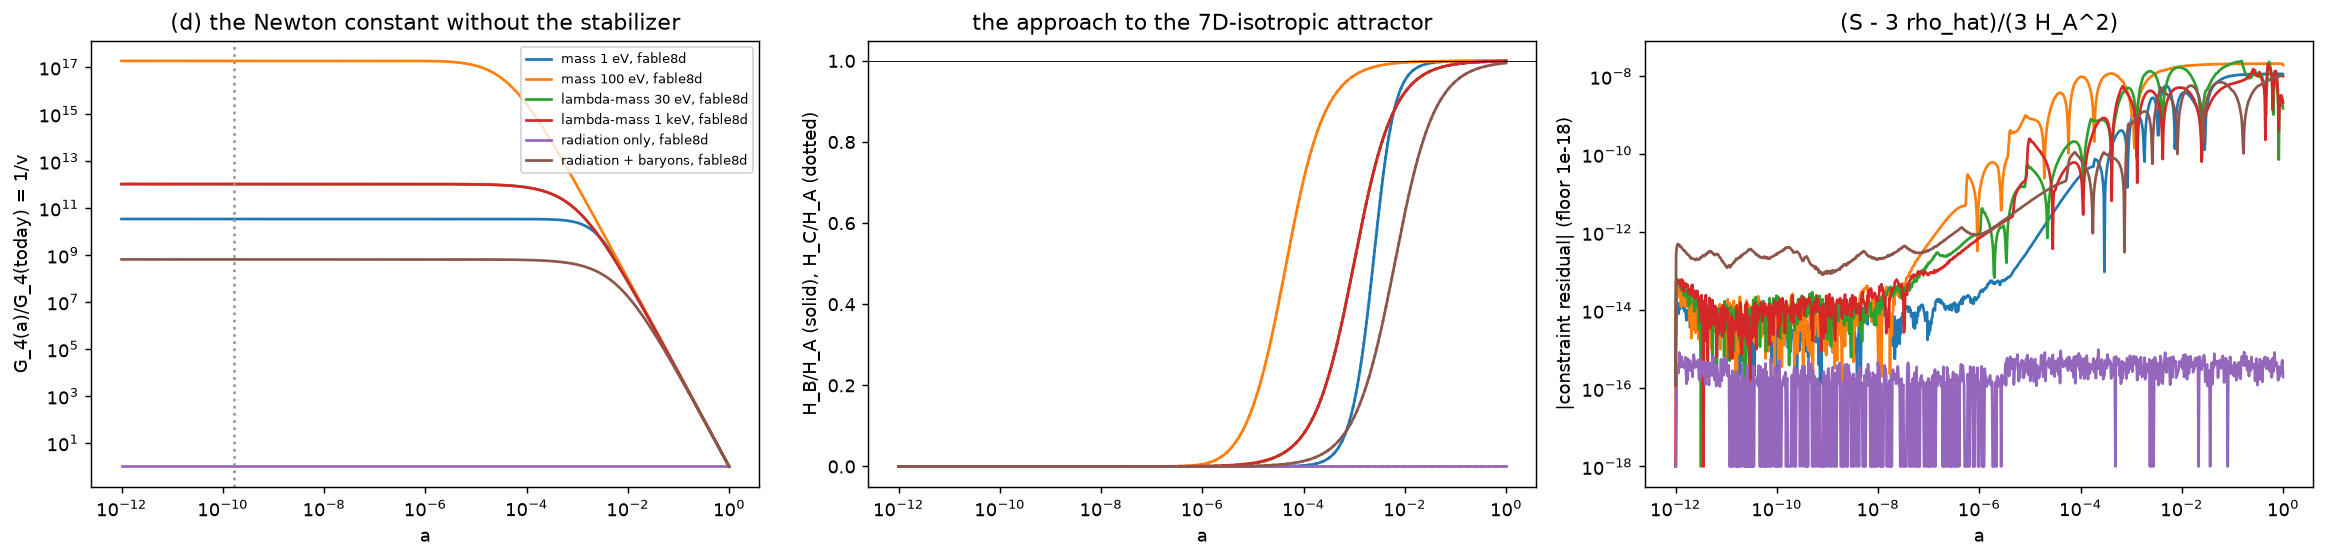
\includegraphics[width=\linewidth]{nb06_d_nogo_8d.png}
  \caption{\texttt{fable-cosmology/\allowbreak results/\allowbreak nb06\_d\_nogo\_8d.png} (notebook 06, section 5.8), runs (d):
  $G_4(a)/G_4(\text{today})=1/v$, $H_B/H_A$ and $H_C/H_A$ (the approach to the 7-dimensional isotropic
  attractor), and the constraint residual $(S-3\hat\rho)/(3H_A^2)$.}
  \label{fig:nb06d}
\end{figure}

\subsection{The cases the solver refuses, and why}
\label{sec:9.11}

Each exits with code 1 and one line of physical reason \cfnb{nb06 \S5.9}:
\begin{Verbatim}[fontsize=\scriptsize]
$ fable_fermion fable4d --potential lorentz --points 1001
  exit code 1: fable_fermion: rho_hat = H_A^2 <= 0 from N = -0.7597808064 (a = 0.4677689478) on: the Kohn-Sham ground state has negative energy there (m_eff = -3.802078e-2, sigma8 = -9.789374e-4, rho_f = -4.830421e-1 (U = -4.847891e-1) against rho_r + rho_b = 4.830421e-1); H_A^2 = rho_hat is impossible (the onset located past the last accepted CVODE step and bisected)
$ fable_fermion fable4d --potential quadratic --param gq=0.5 --points 1001
  exit code 1: fable_fermion: gap-branch jump (sign of m_eff) between N = -0.027631021115929855 and N = 0: m = -3.1667192351800344e-1 -> 4.060727073199006e2: a first-order transition of the Kohn-Sham ground state; the RHS is discontinuous there and energy conservation would need the Maxwell construction, which this solver does not implement
$ fable_fermion fable8d --potential mass --direction backward
  exit code 1: fable_fermion: fable8d runs forward only (design review E4): backward in time the shear modes grow as A^-3 v^-1 relative to H_A ~ A^-2, the solution runs to the 8D Kasner point H_B/H_A = -0.2929 and the constraint drifts to O(1); use fable4d --direction backward
all three refused with exit code 1 and the expected reason
\end{Verbatim}
\cfcode{lorentz}: the Kohn--Sham ground state moves to the negative-$\sigma$ branch, whose energy is negative (a
well of $W$ on $\sigma<0$ that the quantum gas reaches and the classical $s\geq0$ field never did). Repulsive
\cfcode{quadratic}: a first-order transition (\secref{sec:8.1}). \texttt{fable8d} backward: the constraint grows
backward (\secref{sec:5.4}). (These lines are the notebook's execution of 22:53 PDT. The solver commit
\cfcode{2bc936d} of 23:12 detects both the negative-energy onset and the gap-branch jump inside the right-hand
side, on every internal CVODE step, and bisects them to adjacent doubles, independently of the output grid:
its message records \cfcode{lorentz} at $a=0.4677689478$ ``whatever \cfcode{--points} is'' and the
repulsive-quadratic jump at $a=0.9962806544$ ``for any grid'', with scipy agreeing to $8\times10^{-12}$. The
quadratic line above brackets the jump only between two output rows; the re-executed notebook 06 is expected to
print the bisected location instead, and its output is the record.)

\subsection{Three implementations, one answer: CVODE, scipy and Mathematica}
\label{sec:9.12}

\paragraph{Part~VIII's own solution.} Section~33 solves two \texttt{fable4d} cases in Mathematica,
independently of the reference script: every tenth row (71 of 701) by exact algebra from Section~29's closed
forms (with \cfcode{FindRoot} for the gap), the age of \cfcode{mass30eV} by \cfcode{NIntegrate} between the rows,
and the age of \cfcode{power} by \cfcode{NDSolve} of the pair $(m(N),\ln t(N))$ with the \textbf{differentiated}
gap equation
\[
  \frac{dm}{dN}=-\frac{W''(\sigma)\,(\partial\sigma/\partial\kF)\,\kF}{1-W''(\sigma)\,\partial\sigma/\partial m}
\]
instead of solving it \cfprose{VIII \S33}. The run printed \cfdisplayed{VIII \S33},
\file{claude-fable/run_fermion_fable_part8.log}:
\begin{Verbatim}[fontsize=\scriptsize]
  [0.242 s]  fable4d mass30eV: 71 rows by exact algebra, the age by NIntegrate between the rows
  [0.603 s]  fable4d power: NDSolve of (m(N), ln t(N)) with the differentiated gap equation
  [0.047 s]  fable4d power: 71 rows by exact algebra (FindRoot of the gap at every row)
  mass30eV: m0 = 30 eV = 12182.18122 E_c;  kF0 = 0.0544035545089 E_c = 0.00013397491 eV;  V0 = 0.6856647126;  a_nr = kF0/m0 = 4.46583e-6;  t0 = 0.951246513195 / H0
  power:    m_today = 100 eV;  kF0 = 0.0464558024014 E_c;  lam = 217.736704888;  m0 = 27.15187044 eV;  U_today = 0.4006647126;  w_f(1) = -0.421457436338;  t0 = 0.9218031611 / H0
  P_stab(a) [units of rho_c0] at a = 1e-10, 1e-6, 1e-3, 1:   mass30eV {-2.4626e28, -6.53147e16, -1.57121e8, -0.842786};   power {-2.46243e28, -4.87299e16, -9.93078e7, -0.700286}
\end{Verbatim}
and asserted \cfproved{VIII \S33}
\begin{itemize}
  \item \cfL{fable4d RUNS [THE RESULT]: mass30eV -- flat today (H\_A(1) == 1), eps\_KS(1) == 0.265, ultra-relativistic at the start (w\_f(a\_i) = 1/3 to 1e-8), non-relativistic at a\_nr = kF0/m0 == 4.16e-4 (m/eV)\textasciicircum{}(-4/3) (1\%), and w\_f >= -1 at every row}
  \item \cfL{fable4d RUNS [THE RESULT]: power -- flat today, m\_eff(1) == 100 eV, m0 == 27.15 eV > 0, m\_eff INCREASES monotonically from m0 (early) to m\_today, and w\_f >= -1 at every row}
  \item \cfL{fable4d RUNS [has content]: the differentiated gap equation carries m(N) along the history -- NDSolve's m agrees with the per-row FindRoot to 1e-15 at all 71 rows}
  \item \cfL{fable4d RUNS [THE RESULT]: the stabilizer P\_stab = -F\_total/2 is NEGATIVE at every row of both runs -- the null-energy violation along x0 is present along the whole history}
  \item \cfL{fable4d RUNS [fidelity]: the reference CSVs have the expected header and 701 rows}
  \item \cfL{fable4d RUNS [fidelity]: at every tenth row ALL TEN columns agree with fable-cosmology/reference/mathematica\_fable4d\_mass30eV.csv and \_power.csv to 1e-10 (relative; P\_obs\_f relative to rho\_f; N and w\_f absolute)}
\end{itemize}
The comparison with the reference CSVs printed
\cfcode{max difference per column {0., 0., 0., 0., 0., 0., 0., 0., 0., 0.}} for both files (three-digit
formatting). When this log was recorded the Rust CSVs \file{results/nb06_fable4d_mass30eV.csv} and
\file{nb06_fable4d_power.csv} did not yet exist, and the conditional comparison with them was skipped, not
failed (\cfcode{NOTE  Rust CSV not found; that comparison was skipped, not failed}); notebook 06 now writes
them, and the three-way comparison below includes them.

\paragraph{The reference script} \file{fable-cosmology/reference/make_reference_fermion.wls} writes
\file{mathematica_fable4d_mass30eV.csv} and \file{mathematica_fable4d_power.csv}: 701 values of $N$ from
$\ln10^{-10}$ to 0, columns \cfcode{N, a, t, H_A, rho_f, P_obs_f, w_f, m_eff, sigma, kF_over_m}; every row is
exact algebra at 40 significant digits (the power-law gap by Brent's method at 45 digits), the age by
\cfcode{NDSolve} at working precision 30 with the stable series of the Fermi-sea integrals for $\kF/|m|<1/4$
[file: its header].

\paragraph{Three-way} \cfnb{nb06 \S5.5, file \file{results/nb06_threeway.csv}} --- CVODE (Rust), scipy (the
independent implementation), and Mathematica (the reference CSVs), column by column, on both reference cases
(the table of the notebook, transposed: one row per compared column):

{\small
\begin{center}
\begin{tabular}{@{}lll@{}}
\toprule
column & \file{nb06_fable4d_mass30eV} & \file{nb06_fable4d_power} \tabularnewline
\midrule
\multicolumn{3}{@{}l}{\emph{Rust $-$ Mathematica:}} \tabularnewline
$t$ & \texttt{2.352e-09} & \texttt{1.500e-09} \tabularnewline
$H_A$ & \texttt{3.338e-11} & \texttt{3.353e-11} \tabularnewline
$\rho_f$ & \texttt{1.271e-14} & \texttt{5.540e-14} \tabularnewline
$P_{\mathrm{obs},f}$ & \texttt{1.603e-13} & \texttt{6.990e-13} \tabularnewline
$\meffx$ & \texttt{1.792e-15} & \texttt{5.032e-14} \tabularnewline
$\sigma$ & \texttt{9.938e-15} & \texttt{5.242e-14} \tabularnewline
$\kF/m$ & \texttt{6.506e-15} & \texttt{5.128e-14} \tabularnewline
$w_f$ (abs) & \texttt{3.608e-15} & \texttt{8.160e-15} \tabularnewline
\multicolumn{3}{@{}l}{\emph{scipy $-$ Mathematica:}} \tabularnewline
$H_A$ & \texttt{3.347e-11} & \texttt{3.362e-11} \tabularnewline
$\rho_f$ & \texttt{1.419e-12} & \texttt{1.362e-12} \tabularnewline
$P_{\mathrm{obs},f}$ & \texttt{1.172e-12} & \texttt{1.170e-12} \tabularnewline
$\meffx$ & \texttt{2.986e-16} & \texttt{4.586e-14} \tabularnewline
$t(A=1)$ & \texttt{2.665e-14} & \texttt{4.241e-14} \tabularnewline
\bottomrule
\end{tabular}
\end{center}
}

\noindent\cfcode{written: results/nb06_threeway.csv;  CVODE, scipy and Mathematica agree to better than 1e-6 on both reference cases};
in the power case $\meffx$ runs from \cfcode{27.1519 eV (a = 1e-10) to 100.0000 eV (today)}.

\paragraph{Every run re-computed independently} \cfnb{nb06 \S5.10, file \file{results/nb06_crosscheck.csv}}:
the independent implementation takes the normalized parameters from the \cfL{\# params:} line of each CSV and
re-computes the run --- every Fermi-sea integral by adaptive quadrature, every gap root by \cfcode{brentq},
\texttt{fable8d} by DOP853 at \cfcode{rtol = 1e-11}, \texttt{fable4d} algebraically with $t(A=1)$ by adaptive
quadrature --- and checks the Friedmann consistency of the solver's columns and the covariant conservation of
the independently computed fluid (Richardson-extrapolated central differences). The notebook fails if any
difference exceeds $10^{-6}$. It printed
\cfcode{largest difference over the 29 kept runs: 1.08e-08;  over the 90 scan runs: 4.43e-09;  largest conservation residual of the independent fluid: 1.24e-07}.

\subsection{The consolidated table of every kept run}
\label{sec:9.13}

\cfnb{nb06 \S5.11, files \file{results/nb06_runs.csv} (29 rows, 34 columns), \file{results/nb06_cpl_fits.csv}},
verbatim (on the next page, which is turned to landscape so that its lines fit):

\begin{landscape}
\begin{center}
\small\textbf{The consolidated table of every kept run, as notebook 06 printed it (its section 5.11)}
\end{center}
\begin{Verbatim}[fontsize=\scriptsize,xleftmargin=0pt]
run                                 m [eV]      a_nr dNeff BBN           CPL w_f      CPL w_DE,inf   min cs2 vac/rho a>=.3 G(a_i)/G(1) |Gdot/G| /yr
mass 1 eV (EdS)                          1  0.000637     36.75 (-0.000, +0.000) (+nan, +nan)  1.35e-07     0.000e+00   1.000e+00    0.000e+00
mass 30 eV (EdS)                        30  6.84e-06    0.3943 (-0.000, +0.000) (+nan, +nan)  1.56e-11     0.000e+00   1.000e+00    0.000e+00
mass 100 eV (EdS)                      100  1.37e-06   0.07918 (-0.000, +0.000) (+nan, +nan)  6.28e-13     0.000e+00   1.000e+00    0.000e+00
mass 1000 eV (EdS)                    1000  6.37e-08  0.003675 (-0.000, +0.000) (+nan, +nan)  1.35e-15     0.000e+00   1.000e+00    0.000e+00
mass 2000 eV (EdS)                    2000  2.53e-08  0.001459 (-0.000, +0.000) (+nan, +nan)  2.13e-16     0.000e+00   1.000e+00    0.000e+00
lambda-mass 30 eV                       30  4.47e-06   0.07179 (-0.757, +1.010) (-1.000, +0.000)  6.65e-12     0.000e+00   1.000e+00    0.000e+00
lambda-mass 100 eV                     100  8.97e-07   0.01442 (-0.757, +1.010) (-1.000, +0.000)  2.68e-13     0.000e+00   1.000e+00    0.000e+00
lambda-mass 1000 eV                   1000  4.16e-08 0.0006692 (-0.757, +1.010) (-1.000, +0.000)  5.78e-16     0.000e+00   1.000e+00    0.000e+00
lambda-mass 2000 eV                   2000  1.65e-08 0.0002656 (-0.757, +1.010) (-1.000, +0.000)   9.1e-17     0.000e+00   1.000e+00    0.000e+00
lambda-mass 30 eV (reference)           30  4.47e-06   0.07179 (-0.757, +1.009) (-1.000, +0.000)  6.65e-12     0.000e+00   1.000e+00    0.000e+00
power nu=0.236, 30 eV                   30  2.22e-05   0.07179 (-0.783, +0.445) (-0.082, -7.986)    -0.611     1.314e+13   1.000e+00    0.000e+00
power nu=0.236, 100 eV                 100  4.47e-06   0.01442 (-0.783, +0.445) (-0.082, -7.986)    -0.611     1.622e+15   1.000e+00    0.000e+00
power nu=0.5, 30 eV                     30     0.669   0.07179 (-0.804, -0.358) (-0.249, -10.191)       -27     2.229e+14   1.000e+00    0.000e+00
power nu=0.5, 100 eV                   100     0.669   0.01442 (-0.804, -0.359) (-0.249, -10.191)       -27     2.752e+16   1.000e+00    0.000e+00
expdamp xt=1/2.21, 30 eV                30     0.712   0.07179 (-0.829, -0.317) (-0.128, -11.778)     -21.8     2.327e+14   1.000e+00    0.000e+00
expdamp xt=1/2.21, 100 eV              100     0.712   0.01442 (-0.829, -0.317) (-0.128, -11.779)     -21.8     2.873e+16   1.000e+00    0.000e+00
quadratic gq=-0.5, 30 eV                30     0.643   0.07179 (-0.730, -0.483) (-0.180, -9.321)     -47.1     2.031e+14   1.000e+00    0.000e+00
quadratic gq=-0.5, 100 eV              100     0.643   0.01442 (-0.730, -0.483) (-0.180, -9.321)     -47.1     2.508e+16   1.000e+00    0.000e+00
power nu=0.5, 100 eV, Omega_qp0=0.55     100  4.21e-06   0.03817 (-0.448, +0.264) (-0.327, -9.682)    -0.364     2.350e+14   1.000e+00    0.000e+00
power nu=0.236, 1 eV (Delta N_eff)       1   0.00207     6.692 (-0.783, +0.445) (-0.082, -7.985)    -0.611     1.622e+07   1.000e+00    0.000e+00
power nu=0.5, 1 eV (Delta N_eff)         1      0.67     6.692 (-0.807, -0.347) (-0.251, -10.172)     -21.7     2.720e+08   1.000e+00    0.000e+00
expdamp xt=1/2.21, 1 eV (Delta N_eff)       1     0.712     6.692 (-0.832, -0.305) (-0.130, -11.753)     -21.7     2.850e+08   1.000e+00    0.000e+00
quadratic gq=-0.5, 1 eV (Delta N_eff)       1     0.643     6.692 (-0.732, -0.473) (-0.182, -9.306)     -46.4     2.490e+08   1.000e+00    0.000e+00
mass 1 eV, fable8d                       1   0.00124     521.5 (-0.000, +0.000) (+0.394, -8.104)  3.93e-07     0.000e+00   3.438e+10    2.757e-10
mass 100 eV, fable8d                   100  2.66e-06     1.124 (-0.000, +0.000) (+0.394, -8.104)  1.83e-12     0.000e+00   1.852e+17    2.757e-10
lambda-mass 30 eV, fable8d              30  4.47e-06   0.07179 (-1.103, +1.715) (-1.716, +5.459)  5.13e-12     0.000e+00   1.046e+12    2.757e-10
lambda-mass 1 keV, fable8d            1000  4.16e-08 0.0006692 (-1.103, +1.715) (-1.716, +5.459)  4.46e-16     0.000e+00   1.067e+12    2.757e-10
radiation only, fable8d                nan       nan         0 (+nan, +nan) (+nan, +nan)       nan     0.000e+00   1.000e+00    0.000e+00
radiation + baryons, fable8d           nan       nan         0 (+nan, +nan) (+0.386, -8.020)       nan     0.000e+00   6.540e+08    2.310e-11
\end{Verbatim}
\end{landscape}

\noindent(The \cfcode{vac/rho} column is \texttt{0} for constant-mass runs, where the sea energy is a constant
absorbed into $V_0$.)

\subsection{The figures}
\label{sec:9.14}

All written by notebook 06 under \file{fable-cosmology/results/} (and those of notebook 05, which show the
fluid itself):

{\small
\renewcommand{\arraystretch}{1.25}
\begin{center}
\begin{tabular}{@{}>{\raggedright\arraybackslash}p{0.34\linewidth}>{\raggedright\arraybackslash}p{0.6\linewidth}@{}}
\toprule
figure & what it shows \tabularnewline
\midrule
\file{nb06_a_mass_wdm.png} (figure~\ref{fig:nb06a}) & runs (a): the author's mass term, $\wDM=\PKS/\epsKS$ ($=w_f$ there) against $a$: the degenerate fable cools from $1/3$ to 0 \tabularnewline
\file{nb06_b_lambda_mass.png} (figure~\ref{fig:nb06b}) & runs (b): $w_f$ (solid) and $\wDM$ (dotted); and $\wDE+1$ on $0.3\leq a\leq1$: the inferred dark energy is a cosmological constant \tabularnewline
\file{nb06_c_de_potentials.png} (figure~\ref{fig:nb06c1}) & runs (c): $w_f$ (never below $-1$), the observer's $\wDE$ (clipped to $[-3,1]$, poles and crossings marked), $\meffx/\mtoday$, and $c_s^2$ (negative below the line) \tabularnewline
\file{nb06_c_exchange_vacuum_stabilizer.png} (figure~\ref{fig:nb06c2}) & runs (c): $\wDM$ and $\wDMeff$, the exchange $Q$, the Dirac-sea energy relative to the total density, and $\Pstab/\rho$ \tabularnewline
\file{nb06_scan.png}, \file{nb06_scan_cpl.png} (figures~\ref{fig:nb06scan}, \ref{fig:nb06scancpl}) & the scans: per family, the smallest $\meffx/\mtoday$ over $10^{-3}\leq a\leq0.3$ and the smallest $c_s^2$ ($a\geq10^{-3}$) against the scanned parameter; the CPL points $(w_0,w_a)$ of $\wDE$ (fitted above its poles) and of $w_f$ \tabularnewline
\file{nb06_dm_mass_bounds.png} (figure~\ref{fig:nb06dm}) & the free streaming of a degenerate fable: $v_{\mathrm{rms}}$ today against the fable mass, with the warm-dark-matter velocities \tabularnewline
\file{nb06_d_nogo_8d.png} (figure~\ref{fig:nb06d}) & runs (d): $G_4(a)/G_4(\text{today})=1/v$, $H_B/H_A$ and $H_C/H_A$ (the approach to the 7-dimensional isotropic attractor), and the constraint residual $(S-3\hat\rho)/(3H_A^2)$ \tabularnewline
\file{nb05_w_ks.png}, \file{nb05_ks_accuracy.png}, \file{nb05_classical_vs_quantum.png}, \file{nb05_gap_roots.png}, \file{nb05_minimax.png}, \file{nb05_preuniverse_cooling.png}, \file{nb05_vacuum_energy.png} (figures~\ref{fig:nb05wks}, \ref{fig:nb05ks}, \ref{fig:nb05cq}, \ref{fig:nb05gap}, \ref{fig:nb05minimax}, \ref{fig:nb05cool}, \ref{fig:nb05vac}) & the Kohn--Sham fluid: $w_{\KS}(x)$, the accuracy of the stable forms, classical vs quantum $w$, the gap roots, the minimax and Walecka functionals, the cooling on the pre-universe, the Dirac-sea energy \tabularnewline
\bottomrule
\end{tabular}
\end{center}
}

\begin{figure}[tbp]
  \centering
  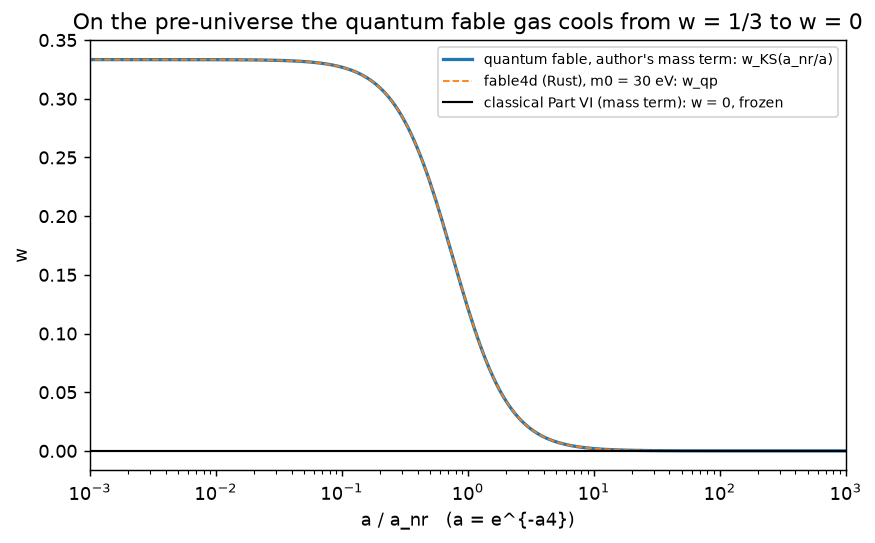
\includegraphics[width=0.75\linewidth]{nb05_preuniverse_cooling.png}
  \caption{\texttt{fable-cosmology/\allowbreak results/\allowbreak nb05\_preuniverse\_cooling.png} (notebook 05): the cooling on the
  pre-universe --- the quantum fable gas of the author's mass term goes from $w=1/3$ to $w=0$ as the observed
  sheet expands, while the classical Part~VI fable's $w=0$ is frozen (\secref{sec:3.6}).}
  \label{fig:nb05cool}
\end{figure}

\FloatBarrier

% ===============================================================================================
\section{The answers to [1] and [2]}
\label{sec:10}

The author asked: \textbf{[1]} ``Does this system provide a physical mechanism for a time-varying dark energy
equation of state (w)?'' \textbf{[2]} ``[\dots] time-varying dark matter equation of state (w)?'' The answers
below rest on the runs of \secref{sec:9} and the theorems of sections~\ref{sec:4}--\ref{sec:7}. Notebook 06
composes its own statement of the answers from its tables and asserts every qualitative claim in it; its
headlines read \cfnb{nb06 \S7}: ``\textbf{Formally yes, in the stabilized model, but in none of the runs is it
a viable one.}'' for [1], and ``\textbf{Yes, intrinsically, but for an allowed mass the variation is over long
before recombination.}'' for [2].

\subsection{Answer [1]: a time-varying dark-energy equation of state}
\label{sec:10.1}

\textbf{Yes, as a mechanism --- in the stabilized model, and only with a mass-varying potential. None of the
runs is a viable cosmology, and the mechanism carries every one of the following caveats.}

\paragraph{What the mechanism is.} In the Kohn--Sham ground state the fable's energy is
$\rho=\rho_{\mathrm{qp}}+\rho_U$, and the mean-field condensate $\rho_U=W(\sigma_7)-\sigma_7W'(\sigma_7)$ has
$P=-\rho_U$ along all seven spatial directions: a vacuum energy. When $W$ is not linear, $\rho_U$ changes as the
density falls, the quasiparticle mass $\meffx=W'(\sigma_7)$ changes with it, and the two parts exchange energy at
the rate $Q=\sigma_8\,dm/dt$ (\secref{sec:7.10}). The dark energy that an observer infers therefore varies in
time. For a massive power law $W=m_0\sigma+\lambda\sigma^\nu$ it is, in closed form and confirmed by the runs to
$1.2\times10^{-9}$,
\[
  \wDE(a)=-\frac{1-\nu}{1-\nu\,a^{-3(1-\nu)}},
\]
with a pole at $a=\nu^{1/(3(1-\nu))}$ ($0.5326$ for $\nu=0.236$) (\secref{sec:9.7}). The observer's CPL fits of
the eight dark-energy runs of \secref{sec:9.6} lie at distances from the supernova fit
$(w_0,w_a)=(-0.861,-0.60)$ of $7.43$ (\cfcode{power} $\nu=0.236$: $(-0.082,-7.986)$) to $11.2$ (\cfcode{expdamp}:
$(-0.128,-11.778)$) [file: \file{fable-cosmology/results/nb06_cpl_fits.csv}], and the fits are not faithful,
because $\wDE$ has a pole inside $0.3\leq a\leq1$ in all of them.

\paragraph{What does not give it.} With the author's mass term alone there is no dark energy at all: the fable
is a free gas that closes the budget, an Einstein--de Sitter-like universe with $\Omega_{f0}=0.95066$ and
$q_0=0.50005$ (\secref{sec:9.4}). With a mass term plus a bare $V_0$ (\cfcode{lambda-mass}), the observer infers
\textbf{exactly a cosmological constant}: CPL $(w_0,w_a)=(-1.000000,\,+1.3\times10^{-9})$,
$(-1.000000,\,+5.3\times10^{-11})$, $(-1.000000,\,+1.2\times10^{-13})$, $(-1.000000,\,+1.7\times10^{-14})$ at 30,
100, 1000, 2000\,eV --- no time variation (\secref{sec:9.5}). $V_0$ is a bare cosmological constant and is
reported as such.

\paragraph{The caveats, each quantified:}
\begin{enumerate}
  \item \textbf{No true phantom --- but an apparent phantom and phantom crossing in the observer's fit.} The
        fable's own equation of state never goes below $-1$: $\rho+\Pobs=\wF n/v\geq0$ is an identity
        (\secref{sec:7.9}), and the smallest $w_f$ over every run is \texttt{-0.9999987921}. The classical
        Part~VI crossing of $-1$ (at $V'(s^*)=0$, \secref{sec:2.12.7}) does \textbf{not} survive quantization.
        The \textbf{observer-inferred} dark energy, however, is phantom or crosses $-1$ inside $0.3\leq a\leq1$
        in 9 of 9 runs of \secref{sec:9.6} and in 90 of 90 scan points: subtracting cold dark matter with
        today's mass when the mass was different leaves
        $\rho_{\mathrm{DE}}+P_{\mathrm{DE}}\approx\bigl(\meffx(a)-\mtoday\bigr)\,n$, negative whenever $\meffx$
        grows (the mechanism of Das, Corasaniti and Khoury, Phys.\ Rev.\ D \textbf{73}, 083509 (2006)), with no
        phantom field. For the massive power law the crossing lies in the last output interval before today
        ($a>0.9727$), where the quasiparticles' kinetic energy, of relative size $\tfrac{3}{10}(\kF/m)^2$, finally
        exceeds $\bigl(\mtoday-\meffx(a)\bigr)\,n$ \cfnb{nb06 \S7}.
  \item \textbf{Mass-varying dark energy with massive dark matter needs a power law with $\nu<0.279$.} In the
        scans 28 of 90 points keep the fable massive over $10^{-3}\leq a\leq0.3$, all of them power laws; every
        \cfcode{quadratic} and \cfcode{expdamp} point is a massless gas (radiation) until late times and supplies
        no dark matter at recombination. A power law stays massive exactly when its bare mass $m_0$ is positive,
        i.e.\ when $\Omegaqp/U_t>\nu/(1-\nu)$; with the observed split $\Omegaqp=0.265$ that is $\nu<0.2788$
        (\secref{sec:9.8}). The massive mass-varying example with a larger quasiparticle share (Part~VIII's
        case: \cfcode{power}, $\nu=0.5$, $\mtoday=100$\,eV, $\Omegaqp=0.55$, no bare Lambda) has $\meffx$ rising
        from 27.15\,eV to 100.00\,eV, $w_f$ today $-0.4215$, $q_0=-0.1010$, and matter today
        $\Omegaqp+\Omega_{b0}=0.599$, about twice the measured $\Omega_m\approx0.315$ (Planck 2018): it is
        massive because its dark matter outweighs its dark energy, which the observed universe does not allow
        \cfnb{nb06 \S7}.
  \item \textbf{It is adiabatically unstable.} Every scan point that stays massive has $c_s^2<0$ after
        $a=10^{-3}$ (smallest $c_s^2$ between $-0.647$ and $-0.056$), and so do all 9 runs of \secref{sec:9.6}
        ($-0.611$ for $\nu=0.236$, $-0.364$ for Part~VIII's case, down to $-47.1$ for \cfcode{quadratic}). This is
        the adiabatic instability of mass-varying fermions (as found by Afshordi, Zaldarriaga and Kohri for
        mass-varying neutrinos).
  \item \textbf{The Dirac-sea vacuum energy demands a fine-tuning.} The renormalized sea energy that the no-sea
        functional drops changes, for a mass variation of order $m$, by $g\,m^4/(64\pi^2)$: $3.44$,
        $3.44\times10^{4}$, $3.44\times10^{8}$, $3.44\times10^{12}$ times $\rhoc$ at $m=0.01$, $0.1$, $1$, $10$\,eV,
        more than the critical density for $m>7.341$\,meV (\secref{sec:7.11}). Along every mass-varying run it
        changes by $\boldsymbol{1.31\times10^{13}}$ \textbf{to} $\boldsymbol{2.87\times10^{16}}$ \textbf{times the
        total density at $a\geq0.3$} (over the scans at least $3.79\times10^{9}$) \cfnb{nb06 \S7}. The runs read
        $W$ as the fully renormalized effective potential, which absorbs the sea energy only by fine-tuning the
        bare potential against it to that precision. The cosmological-constant problem is not solved.
  \item \textbf{It needs the stabilizer, which violates the null energy condition.} All of this holds with the
        hidden sheet held by $\Pstab=-F/2$ (today $-0.8428\,\rhoc$ in the $\Lambda$CDM-like runs, $-0.7003$ in
        Part~VIII's power case), a Lagrange multiplier, not a stress derived from any field, with zero energy
        density; it violates the null energy condition along $x_0$ on 100.0\,\% of the output rows of every
        stabilized run (\secref{sec:9.1}).
  \item \textbf{Without the stabilizer it is excluded (the \texttt{fable8d} no-go).} Left free, the hidden sheet
        is driven by dust and vacuum energy to the 7-dimensional isotropic attractor, and the observed Newton
        constant $G_4=G_8/\Vhidx$ varies: $G(a_i)/G(1)=$ $3.44\times10^{10}$, $1.85\times10^{17}$,
        $1.05\times10^{12}$, $1.07\times10^{12}$ in the four fable runs and $6.54\times10^{8}$ for radiation plus
        baryons alone; $\Delta G/G$ since nucleosynthesis is $-1$ (against about $0.1$), and $|d\ln G/dt|$ today
        $\geq2.31\times10^{-11}$\,/yr (against the lunar-laser-ranging bound $10^{-13}$\,/yr)
        (\secref{sec:9.10}). The only frozen-compatible Kohn--Sham fable is radiation (\secref{sec:7.7}).
  \item \textbf{The split into dark matter and dark energy is a convention.} The condensate $\rho_U$ is an
        8-dimensional vacuum energy, with $P=-\rho_U$ along the hidden directions as well; calling it dark
        energy and the quasiparticles dark matter is a choice of bookkeeping (\secref{sec:7.4}).
  \item \textbf{The approximations under which all of this holds:} semiclassical gravity
        ($G=\kappa\langle\That\rangle$); the Kohn--Sham mean field with exchange--correlation neglected
        (\secref{sec:7.12}); zero modes along $x_0$ and the hidden timelike sheet, with $x_0$ compactified (a
        Kaluza--Klein gap above the temperatures considered) and the hidden timelike sheet a formal comoving
        volume (compactifying it gives closed timelike curves); the asymptotic Bianchi-I reading of the
        primordial field, which neglects terms of order $\cot(6Hx_0)$ and $\cot^2(6Hx_0)$ (\secref{sec:5.3});
        $g_*(T)$ not followed.
\end{enumerate}

\subsection{Answer [2]: a time-varying dark-matter equation of state}
\label{sec:10.2}

\textbf{Yes, intrinsically: the quantized fable's dark-matter equation of state runs from $1/3$ to 0. For an
allowed mass the variation is over long before recombination.}
\begin{enumerate}
  \item \textbf{The mechanism.} The fable's quasiparticles are a degenerate Fermi gas ($g=8$ states per
        momentum), and their equation of state is $\wDM=\PKS/\epsKS$, a function of $x=\kF/|m|$ alone that rises
        monotonically from 0 (dust) to $1/3$ (radiation) (\secref{sec:3.6}). As the universe expands,
        $\kF=k_{F0}/a$ falls, and $\wDM$ falls from $1/3$ to 0: \textbf{a time-varying dark-matter equation of
        state}, which is a property of the quantum gas and has no counterpart in the classical Part~VI fable
        (whose $w$ was frozen on the pre-universe and 0 for the mass term). Every run starts at
        $\wDM=0.333333$ and ends today at most $8.1\times10^{-8}$ \cfnb{nb06 \S7}; the transition is at
        $\anr=k_{F0}/m$, $4.466\times10^{-6}$ for 30\,eV and $4.163\times10^{-8}$ for 1\,keV, scaling as
        $m^{-4/3}$ (sections~\ref{sec:9.4}--\ref{sec:9.5}). The same cooling happens on the pre-universe itself,
        on the canonical frame with $a_4$ free, whenever the observed sheet expands ($a_4'<0$, \secref{sec:3.6}).
  \item \textbf{How heavy it must be, and hence when the variation happens.} A fable that is all of the dark
        matter is radiation before $\anr$: $\DNeff(\mathrm{BBN})=6.692\,(m/\mathrm{eV})^{-4/3}<0.3$ requires
        $m>10.3$\,eV ($<0.2$: $m>13.9$\,eV). Free streaming is far more restrictive: matching the rms velocity of
        the Lyman-alpha-allowed thermal warm dark matter requires $m\approx1125$--$1807$\,eV
        (${\sim}1.1$--$1.8$\,keV, a velocity-matching estimate, not a transfer-function computation), and the
        Tremaine--Gunn phase-space bound for illustrative dwarf spheroidals gives $m>231$--$358$\,eV
        (\secref{sec:9.9}). At such masses the change of $\wDM$ from $1/3$ to 0 happens around
        $\anr=4.16\times10^{-8}$ (1\,keV) or $1.65\times10^{-8}$ (2\,keV): \textbf{indistinguishable from cold dark
        matter in the late universe}.
  \item \textbf{With a mass-varying potential the effective equation of state varies late.} The quasiparticles
        then exchange energy with the condensate ($Q=\sigma_8\,dm/dt$), and their effective equation of state
        $\wDMeff=\wDM-\sigKS\,(dm/dN)/(3\epsKS)$ ranges, after $a=10^{-3}$, over $[-0.611,\,+9.85\times10^{-5}]$
        (\cfcode{power} $\nu=0.236$, 30\,eV), $[-0.611,\,+3.59\times10^{-6}]$ (100\,eV), $[-27.6,\,+0.333]$ and
        $[-27.7,\,+0.333]$ (\cfcode{power} $\nu=0.5$), $[-21.8,\,+0.333]$ (\cfcode{expdamp}), $[-47.1,\,+0.333]$
        (\cfcode{quadratic}), and $[-0.364,\,-3.89\times10^{-5}]$ (Part~VIII's case) (\secref{sec:9.6}). This late
        variation is the same exchange that makes the inferred dark energy vary in [1], and it carries all of
        [1]'s caveats (adiabatic instability, the sea energy, the viability window $\nu<0.2788$).
  \item \textbf{The author's mass term alone is dark matter without dark energy.} $W=m_0\sigma$ gives an
        Einstein--de Sitter-like universe ($q_0=+0.50005$, age 9.67\,Gyr with $H_0=67.4$\,km/s/Mpc), not ours;
        with a bare cosmological constant (\cfcode{lambda-mass}) it is $\Lambda$CDM with fable dark matter
        ($q_0=-0.52845$, age 13.8000\,Gyr) (sections~\ref{sec:9.4}--\ref{sec:9.5}).
  \item \textbf{The same caveats as [1]} apply: the stabilized model with its NEC-violating stabilizer (without
        it the Newton constant varies by $6.5\times10^{8}$ to $1.9\times10^{17}$); the split into dark matter and
        dark energy is a convention; semiclassical gravity, the Kohn--Sham mean field with $E_{\mathrm{xc}}$
        neglected (exact for the author's mass term, which is free), zero modes along the hidden directions,
        the asymptotic reading of the primordial field.
\end{enumerate}

% ===============================================================================================
\section{Every command, in full}
\label{sec:11}

The commands run in Git Bash on Windows 11 (plain POSIX shell; they run the same way on Linux and macOS, with
\file{.venv/bin/python} in place of \file{.venv/Scripts/python.exe} and without the \file{.exe} suffix). The
toolchain recorded in the logs: Wolfram Language 15.0.1 for Microsoft Windows (64-bit) (July 2, 2026), called as
\cfcode{wolframscript} (the first lines of the run log and of \file{waveguide_derivation.log}); Rust with
\cfcode{cargo}; the solver \cfcode{fable_fermion 0.1.0, sundials_rs 7.8.0 (pure Rust), CVODE BDF}; Python~3 in the
virtual environment \file{fable-cosmology/.venv} (numpy, scipy, matplotlib, jupyter); MiKTeX with
\cfcode{latexmk} for the LaTeX twin.

\subsection{Set up, and build the solver}
\label{sec:11.1}

\begin{Verbatim}
cd "$(git rev-parse --show-toplevel)"
bash fable-cosmology/setup.sh
\end{Verbatim}
\file{setup.sh} (idempotent) creates \file{fable-cosmology/.venv} and installs \file{requirements.txt} into it,
printing \cfcode{python ok: numpy <v> scipy <v> matplotlib <v>}; makes a sparse clone of the rustSolveIt
repository for this platform (\cfcode{rustSolveIt_Win11_SUNDIALS_7_8_0} on Windows,
\cfcode{rustSolveIt_macos-silicon_SUNDIALS_7_8_0} on Apple-silicon macOS,
\cfcode{rustSolveIt_linux_SUNDIALS_7_8_0} on Linux) into \file{rust/vendor/rustSolveIt}, restricted to its
vendored pure-Rust SUNDIALS 7.8.0 (\cfcode{sundials_rs}), on which the solver crates depend by path; then builds
both solver crates in release mode and runs each with \cfcode{--version}; it ends with
\cfcode{== setup complete} [file: \file{fable-cosmology/setup.sh}]. To rebuild the fermion solver alone:
\begin{Verbatim}
cd "$(git rev-parse --show-toplevel)/fable-cosmology/rust/fable_fermion"
cargo build --release          # -> target/release/fable_fermion(.exe)
./target/release/fable_fermion --version
\end{Verbatim}
which prints \cfcode{fable_fermion 0.1.0, sundials_rs 7.8.0 (pure Rust), CVODE BDF} (the first line of
notebooks 05 and 06). The crate's \file{.cargo/config.toml} pins the FMA instruction on x86-64
(\cfcode{rustflags = ["-C", "target-feature=+fma"]}), which its comment states is REQUIRED by the vendored
\cfcode{sundials_rs} engine, whose deterministic math library uses \cfcode{f64::mul_add}; cargo reads that file
from the directory the build is invoked in.

\subsection{Test the solver}
\label{sec:11.2}

\begin{Verbatim}
cd "$(git rev-parse --show-toplevel)/fable-cosmology/rust/fable_fermion"
cargo test --release
\end{Verbatim}
It runs the unit tests of \file{src/} and the end-to-end tests of \file{tests/cosmology.rs} (each end-to-end
test runs the real binary, writes a CSV and reads it back). At commit \cfcode{c5892bd} (the finished solver)
the commit records \cfcode{cargo test --release: 21 + 8 tests pass (re-run independently)}; at commit
\cfcode{2bc936d} (six defects fixed, 23:12 PDT) it records
\cfcode{34/34 (23 unit + 11 integration, previously 21 + 8)}. The 34 tests [listed from the source files]:

{\small
\begin{longtable}{@{}>{\raggedright\arraybackslash}p{0.2\linewidth}>{\raggedright\arraybackslash}p{0.74\linewidth}@{}}
\toprule
file & tests \tabularnewline
\midrule
\endhead
\file{src/constants.rs} & \file{unit_system_matches_the_standard_values} \tabularnewline
\file{src/cvode_driver.rs} & \file{exponential_decay_forward_and_backward} \tabularnewline
\file{src/numerics.rs} & \file{brent_finds_simple_roots}, \file{gauss_kronrod_is_exact_on_smooth_functions} \tabularnewline
\file{src/potentials.rs} & \file{derivatives_match_finite_differences}, \file{signs_that_the_bracket_proofs_use} \tabularnewline
\file{src/kohn_sham.rs} & \file{fermi_integrals_match_quadrature}, \file{series_and_closed_forms_are_continuous_at_the_switch_points}, \file{nonrelativistic_and_ultrarelativistic_limits}, \file{per_3_volume_mean_field_violates_8d_conservation}, \file{thermodynamic_identities_at_the_self_consistent_point}, \file{derivative_along_the_trajectory_matches_finite_differences}, \file{expdamp_pins_sigma_below_s1_and_mass_goes_to_zero_at_high_density}, \file{multiple_gap_roots_are_found_and_the_lowest_energy_one_is_taken}, \file{quadrature_at_the_review_points_and_switch_continuity}, \file{nonrelativistic_classical_limit_of_the_mean_field}, \file{no_phantom_crossing_rho_plus_p_obs_is_nonnegative}, \file{root_counts_three_for_strong_repulsion_one_for_concave_w}, \file{walecka_functional_is_minimized_at_the_gap_root}, \file{vacuum_energy_vanishes_to_fifth_order_at_the_reference_mass}, \file{vacuum_energy_matches_high_precision_references_near_and_far_from_the_reference_mass}, \file{gap_residual_is_at_round_off_in_massless_phases}, \file{ks_functional_stationary_point_is_a_maximum_for_the_mass_term} \tabularnewline
\file{tests/cosmology.rs} & \file{version_string}, \file{covariant_conservation_along_real_fable8d_runs}, \file{constraint_residual_stays_small_on_forward_fable8d_runs}, \file{frozen_hidden_theorem}, \file{fable8d_with_hidden_frozen_by_hand_reproduces_fable4d}, \file{backward_runs}, \file{physics_checks_along_runs}, \file{negative_energy_refusal_is_found_inside_the_rhs_independently_of_the_output_grid}, \file{first_order_transition_is_found_inside_the_rhs_independently_of_the_output_grid}, \file{gap_residual_and_vacuum_energy_at_round_off_in_1_kev_runs}, \file{insensitivity_to_a_start} \tabularnewline
\bottomrule
\end{longtable}
}

It prints, for each test binary, \cfcode{running N tests}, one \cfcode{test <name> ... ok} line per test, and
\cfcode{test result: ok. N passed; 0 failed; ...}. Its output on the final pushed state is recorded with the
fresh-clone verification of \secref{sec:12}.

\subsection{The unit system, and one gap solve}
\label{sec:11.3}

\begin{Verbatim}
cd "$(git rev-parse --show-toplevel)/fable-cosmology"
F=rust/fable_fermion/target/release/fable_fermion        # fable_fermion.exe on Windows
$F --constants
$F gap --form quadratic --param m0=0.05 --param lam=20 --kf 1
\end{Verbatim}
\cfcode{--constants} prints the unit block quoted in \secref{sec:9.1}. \cfcode{gap} solves the gap equation once
and prints every root with \cfcode{m, sigma8, rho8, P_obs, P_hid, gap_residual} (16 significant digits) and
the selected root; its output for this case is quoted in \secref{sec:8.1}. Notebook 05 also solves the mass term
($m_0=1$, so $\kF=x$) at the fifteen $x=\kF/m$ of its accuracy table (\secref{sec:7.2}), with the arguments
Python's \cfcode{repr} gives:
\begin{Verbatim}
for x in 1e-08 1e-06 0.0001 0.01 0.2 0.25 0.3 0.6 1.0 3.0 10.0 99.0 101.0 10000.0 1000000.0; do
  $F gap --form mass --param m0=1 --kf $x
done
\end{Verbatim}
(the rows \cfcode{sigma8}, \cfcode{rho8}, \cfcode{P_obs} of the mass term are $\sigKS$, $\epsKS$, $\PKS$; they
agree with the independent Python forms to $3.11\times10^{-14}$).

\subsection{Every solver run behind the results of this page}
\label{sec:11.4}

The solver's command line [file: \file{fable-cosmology/rust/fable_fermion/src/main.rs}, module documentation;
prose nb05 \S5, nb06 \S5]:
\begin{Verbatim}[fontsize=\scriptsize]
fable_fermion fable4d|fable8d --potential NAME [--param KEY=VALUE ...] [--direction forward|backward]
              [--a-start A] [--points K] [--out FILE.csv] [--rtol R] [--atol A] [--method bdf|adams]
              [--branch lowest|positive|negative] [--freeze-hidden] [--no-shoot] [--no-fable]
              [--omega-b X] [--omega-r X]
fable_fermion gap --form NAME --param KEY=VALUE ... --kf KF [--v V]
fable_fermion --constants | --version
\end{Verbatim}
\cfcode{--param} keys: \cfcode{mass}: \cfcode{m0_ev}; \cfcode{lambda-mass}: \cfcode{m0_ev}, \cfcode{omega_dm};
\cfcode{power}: \cfcode{m_today_ev}, \cfcode{nu}, \cfcode{omega_dm}; \cfcode{expdamp}: \cfcode{m_today_ev},
\cfcode{xt}, \cfcode{omega_dm}; \cfcode{quadratic}: \cfcode{m_today_ev}, \cfcode{gq}, \cfcode{omega_dm};
\cfcode{lorentz}: \cfcode{m_today_ev}, \cfcode{xt}, \cfcode{omega_dm}. Defaults: \cfcode{--a-start 1e-12},
\cfcode{--points 2001}, \cfcode{rtol 1e-10}, \cfcode{atol 1e-12}, the lowest-energy gap branch,
\cfcode{omega_dm = 0.265}. A run writes a CSV that starts with \cfL{\#} comment lines (the version; a
machine-readable \cfL{\# params:} line with the normalized parameters \cfcode{kf0}, \cfcode{m0}, \cfcode{v0},
\cfcode{lam}, \cfcode{nu}, \cfcode{s1}, \cfcode{lnB_i}, \cfcode{lnC_i}, \cfcode{a_start}, \cfcode{omega_r0},
\cfcode{omega_b0}, \dots; the definition of every column), then a header and one row per output point, 47
columns:
\cfcode{N, a, z, t, B, C, H_A, H_B, H_C, constraint_residual, rho_r, rho_b, rho_f, P_obs_f, P_hid_f, n_f, sigma, m_eff, kF_over_m, w_f, rho_qp, w_qp, rho_U, w_DE_eff, Omega_r, Omega_b, Omega_f, q_dec, G_ratio, cs2_adiabatic, N_eff_extra, P_stab, Omega_sum, rho_DE_inf, w_DE_inf, w_DM_intrinsic, w_DM_eff, Q, rho_DE_eff, F_hidden, dm_dN, m_eff_eV, kF_eV, gap_roots, branch, gap_residual, vac_over_rhoc}.
Its log goes to stderr: the normalization, the result today, \cfcode{a_nr}, \cfcode{DeltaN_eff} at
nucleosynthesis and recombination, the stabilizer's range, the $t(A=1)$ quadrature check, and a
\cfL{\# stats:} line with the CVODE step counts. Exit code 0 is success; 1 a solver or physics error with a
one-line reason; 2 a usage error [prose nb06 \S5].

\paragraph{One complete log} --- the author's mass term at 30\,eV, as notebook 05 ran and printed it
\cfnb{nb05 \S5.7}:
\begin{Verbatim}[fontsize=\scriptsize]
$ fable_fermion fable4d --potential mass --param m0_ev=30 --points 1001 --out results/nb05_fable4d_mass30.csv
  # normalization: closure today (A = B = C = 1): rho_r + rho_b + rho_f = 1; shooting variable [ln kF0 (the fable number density)] = -2.485515249891274e0; rho_f(A=1; kF0) strictly increasing on the Lowest branch over ln kF0 in [-40, 40] (1601 grid points, 0 without a gap solution); unique solution ln kF0 = -2.485515249891274e0
  # fable today (A = 1, v = 1): potential Mass { m0: 12182.181219597018 }, kF0 = 8.3282632088e-2 E_c = 2.050929e-4 eV, m_eff = 1.2182181220e4 E_c = 3.000000e1 eV, rho_qp = 9.5066471258e-1, U = 0.0000000000e0, rho_f = 9.5066471258e-1, w_f = 9.3473556871e-12, gap roots = 1
  # result: H_A(A=1) = 1.000000000000000e0, B(1) = 1.000000000000000e0, C(1) = 1.000000000000000e0, q0 = 5.000460e-1, age t0 = 6.6660643059e-1/H0, max |constraint residual| = 4.303e-16, max |gap residual| = 0.0e0, rows with several gap roots = 0
  # a_nr (kF = |m_eff|) = 6.837070e-6 (z_nr = 1.4626e5), a_eq = 9.2105e-5: WARM / not hot (a_nr between 1e-6 and a_eq)
  # the fable is ultra-relativistic at a_start: kF/|m_eff| = 6.836e6
  # Delta N_eff (fable energy density in units of one massless neutrino species): at BBN (a = 1.6764e-10, T = 1 MeV) = 3.942638e-1, at recombination (a = 9.1659e-4) = 7.048553e1
  # stabilizer: P_stab = -F_hidden/2 ranges over [-2.4622e34, -4.9995e-1] (today -4.999540e-1); it is a Lagrange multiplier with zero energy density and violates the null energy condition along x0 wherever dust is present (rho + P_C = -rho_dust/2)
  # t(A=1) cross-check: CVODE 6.666064305910978e-1 vs Gauss-Kronrod quadrature 6.666064296244345e-1 (rel. diff 1.45e-9, quadrature error estimate 2.4e-14)
  # NOTE: W = m0 sigma alone (no V0): the closure forces Omega_f0 = 1 - Omega_b0 - Omega_r0 = 0.950665: an Einstein-de Sitter-like universe (q0 = 0.5000, +1/2 for pure dust)
  # the DM/DE split (rho_qp = eps/v vs rho_U = W - sigma W') is a convention: the condensate has P = -rho_U in all seven spatial directions, i.e. it is an 8D vacuum energy
  # stats: model=fable4d direction=Forward potential=mass steps=373 rhs_evals=459 nonlin_iters=456 err_test_fails=18 jac_evals=7 wall=0.011s (summed over every CVODE integration of the run, shooting included)
  # fable_fermion 0.1.0, sundials_rs 7.8.0 (pure Rust), CVODE BDF
\end{Verbatim}

\paragraph{Every run,} run from \file{fable-cosmology/} with \cfcode{F} as in \secref{sec:11.3}, in the order the
notebooks ran them, each followed by the \cfL{\# stats:} line it printed (the CVODE steps, right-hand-side
evaluations, Newton iterations, error-test failures, Jacobian evaluations and wall time, summed over every
integration of the run, shooting included), as the notebooks recorded them:
\begin{Verbatim}[fontsize=\scriptsize]
# notebook 05, section 5.7: the author's mass term on the pre-universe (cooling cross-check)
$F fable4d --potential mass --param m0_ev=30 --points 1001 --out results/nb05_fable4d_mass30.csv
#   prints: # stats: model=fable4d direction=Forward potential=mass steps=373 rhs_evals=459 nonlin_iters=456 err_test_fails=18 jac_evals=7 wall=0.011s (summed over every CVODE integration of the run, shooting included)
\end{Verbatim}
\begin{Verbatim}[fontsize=\scriptsize]
# notebook 05, section 5.8: the vacuum-energy column of a mass-varying run
$F fable4d --potential power --param nu=0.236 --param m_today_ev=30 --points 1001 --out results/nb05_fable4d_power0.236_m30.csv
#   prints: # stats: model=fable4d direction=Forward potential=power steps=390 rhs_evals=482 nonlin_iters=479 err_test_fails=20 jac_evals=7 wall=0.010s (summed over every CVODE integration of the run, shooting included)
\end{Verbatim}
\begin{Verbatim}[fontsize=\scriptsize]
# notebook 06, section 5.1: the interval (a_i = 1e-12, 1e-11, 1e-10; CSV to stdout)
$F fable4d --potential lambda-mass --param m0_ev=30 --a-start 1e-12 --points 1001
#   prints: # stats: model=fable4d direction=Forward potential=lambda-mass steps=430 rhs_evals=542 nonlin_iters=539 err_test_fails=25 jac_evals=8 wall=0.010s (summed over every CVODE integration of the run, shooting included)
$F fable4d --potential lambda-mass --param m0_ev=30 --a-start 1e-11 --points 1001
#   prints: # stats: model=fable4d direction=Forward potential=lambda-mass steps=433 rhs_evals=549 nonlin_iters=546 err_test_fails=27 jac_evals=8 wall=0.010s (summed over every CVODE integration of the run, shooting included)
$F fable4d --potential lambda-mass --param m0_ev=30 --a-start 1e-10 --points 1001
#   prints: # stats: model=fable4d direction=Forward potential=lambda-mass steps=438 rhs_evals=525 nonlin_iters=522 err_test_fails=20 jac_evals=8 wall=0.010s (summed over every CVODE integration of the run, shooting included)
$F fable8d --potential lambda-mass --param m0_ev=30 --a-start 1e-12 --points 1001
#   prints: # stats: model=fable8d direction=Forward potential=lambda-mass steps=37544 rhs_evals=42447 nonlin_iters=42339 err_test_fails=654 jac_evals=647 wall=0.040s (summed over every CVODE integration of the run, shooting included)
$F fable8d --potential lambda-mass --param m0_ev=30 --a-start 1e-11 --points 1001
#   prints: # stats: model=fable8d direction=Forward potential=lambda-mass steps=36759 rhs_evals=41619 nonlin_iters=41511 err_test_fails=618 jac_evals=634 wall=0.038s (summed over every CVODE integration of the run, shooting included)
$F fable8d --potential lambda-mass --param m0_ev=30 --a-start 1e-10 --points 1001
#   prints: # stats: model=fable8d direction=Forward potential=lambda-mass steps=34762 rhs_evals=39367 nonlin_iters=39262 err_test_fails=576 jac_evals=593 wall=0.037s (summed over every CVODE integration of the run, shooting included)
\end{Verbatim}
\begin{Verbatim}[fontsize=\scriptsize]
# notebook 06, section 5.2: runs (a), the author's mass term
$F fable4d --potential mass --param m0_ev=1 --points 1001 --out results/nb06_mass_m1_4d.csv
#   prints: # stats: model=fable4d direction=Forward potential=mass steps=392 rhs_evals=480 nonlin_iters=477 err_test_fails=20 jac_evals=7 wall=0.010s (summed over every CVODE integration of the run, shooting included)
$F fable4d --potential mass --param m0_ev=30 --points 1001 --out results/nb06_mass_m30_4d.csv
#   prints: # stats: model=fable4d direction=Forward potential=mass steps=373 rhs_evals=459 nonlin_iters=456 err_test_fails=18 jac_evals=7 wall=0.010s (summed over every CVODE integration of the run, shooting included)
$F fable4d --potential mass --param m0_ev=100 --points 1001 --out results/nb06_mass_m100_4d.csv
#   prints: # stats: model=fable4d direction=Forward potential=mass steps=387 rhs_evals=467 nonlin_iters=464 err_test_fails=16 jac_evals=7 wall=0.011s (summed over every CVODE integration of the run, shooting included)
$F fable4d --potential mass --param m0_ev=1000 --points 1001 --out results/nb06_mass_m1000_4d.csv
#   prints: # stats: model=fable4d direction=Forward potential=mass steps=377 rhs_evals=463 nonlin_iters=460 err_test_fails=19 jac_evals=7 wall=0.010s (summed over every CVODE integration of the run, shooting included)
$F fable4d --potential mass --param m0_ev=2000 --points 1001 --out results/nb06_mass_m2000_4d.csv
#   prints: # stats: model=fable4d direction=Forward potential=mass steps=377 rhs_evals=467 nonlin_iters=464 err_test_fails=18 jac_evals=7 wall=0.010s (summed over every CVODE integration of the run, shooting included)
\end{Verbatim}
\begin{Verbatim}[fontsize=\scriptsize]
# notebook 06, section 5.3: runs (b), lambda-mass, and Part VIII's reference case
$F fable4d --potential lambda-mass --param m0_ev=30 --points 1001 --out results/nb06_lm_m30_4d.csv
#   prints: # stats: model=fable4d direction=Forward potential=lambda-mass steps=430 rhs_evals=542 nonlin_iters=539 err_test_fails=25 jac_evals=8 wall=0.011s (summed over every CVODE integration of the run, shooting included)
$F fable4d --potential lambda-mass --param m0_ev=100 --points 1001 --out results/nb06_lm_m100_4d.csv
#   prints: # stats: model=fable4d direction=Forward potential=lambda-mass steps=418 rhs_evals=515 nonlin_iters=512 err_test_fails=21 jac_evals=8 wall=0.012s (summed over every CVODE integration of the run, shooting included)
$F fable4d --potential lambda-mass --param m0_ev=1000 --points 1001 --out results/nb06_lm_m1000_4d.csv
#   prints: # stats: model=fable4d direction=Forward potential=lambda-mass steps=407 rhs_evals=509 nonlin_iters=506 err_test_fails=21 jac_evals=8 wall=0.010s (summed over every CVODE integration of the run, shooting included)
$F fable4d --potential lambda-mass --param m0_ev=2000 --points 1001 --out results/nb06_lm_m2000_4d.csv
#   prints: # stats: model=fable4d direction=Forward potential=lambda-mass steps=425 rhs_evals=527 nonlin_iters=524 err_test_fails=21 jac_evals=8 wall=0.013s (summed over every CVODE integration of the run, shooting included)
$F fable4d --potential lambda-mass --param m0_ev=30 --param omega_dm=0.265 --a-start 1e-10 --points 701 --out results/nb06_fable4d_mass30eV.csv
#   prints: # stats: model=fable4d direction=Forward potential=lambda-mass steps=429 rhs_evals=548 nonlin_iters=545 err_test_fails=29 jac_evals=8 wall=0.009s (summed over every CVODE integration of the run, shooting included)
\end{Verbatim}
\begin{Verbatim}[fontsize=\scriptsize]
# notebook 06, section 5.4: runs (c), the dark-energy potentials, and Part VIII's mass-varying reference case
$F fable4d --potential power --param nu=0.236 --param m_today_ev=30 --points 1001 --out results/nb06_power_0.236_m30_4d.csv
#   prints: # stats: model=fable4d direction=Forward potential=power steps=390 rhs_evals=482 nonlin_iters=479 err_test_fails=20 jac_evals=7 wall=0.012s (summed over every CVODE integration of the run, shooting included)
$F fable4d --potential power --param nu=0.236 --param m_today_ev=100 --points 1001 --out results/nb06_power_0.236_m100_4d.csv
#   prints: # stats: model=fable4d direction=Forward potential=power steps=401 rhs_evals=505 nonlin_iters=502 err_test_fails=23 jac_evals=7 wall=0.011s (summed over every CVODE integration of the run, shooting included)
$F fable4d --potential power --param nu=0.5 --param m_today_ev=30 --points 1001 --out results/nb06_power_0.5_m30_4d.csv
#   prints: # stats: model=fable4d direction=Forward potential=power steps=430 rhs_evals=551 nonlin_iters=548 err_test_fails=26 jac_evals=8 wall=0.023s (summed over every CVODE integration of the run, shooting included)
$F fable4d --potential power --param nu=0.5 --param m_today_ev=100 --points 1001 --out results/nb06_power_0.5_m100_4d.csv
#   prints: # stats: model=fable4d direction=Forward potential=power steps=433 rhs_evals=545 nonlin_iters=542 err_test_fails=24 jac_evals=8 wall=0.022s (summed over every CVODE integration of the run, shooting included)
$F fable4d --potential expdamp --param xt=0.4524886877828054 --param m_today_ev=30 --points 1001 --out results/nb06_expdamp_m30_4d.csv
#   prints: # stats: model=fable4d direction=Forward potential=expdamp steps=423 rhs_evals=527 nonlin_iters=524 err_test_fails=21 jac_evals=8 wall=0.019s (summed over every CVODE integration of the run, shooting included)
$F fable4d --potential expdamp --param xt=0.4524886877828054 --param m_today_ev=100 --points 1001 --out results/nb06_expdamp_m100_4d.csv
#   prints: # stats: model=fable4d direction=Forward potential=expdamp steps=434 rhs_evals=542 nonlin_iters=539 err_test_fails=23 jac_evals=8 wall=0.020s (summed over every CVODE integration of the run, shooting included)
$F fable4d --potential quadratic --param gq=-0.5 --param m_today_ev=30 --points 1001 --out results/nb06_quadratic_m30_4d.csv
#   prints: # stats: model=fable4d direction=Forward potential=quadratic steps=451 rhs_evals=562 nonlin_iters=559 err_test_fails=23 jac_evals=8 wall=0.011s (summed over every CVODE integration of the run, shooting included)
$F fable4d --potential quadratic --param gq=-0.5 --param m_today_ev=100 --points 1001 --out results/nb06_quadratic_m100_4d.csv
#   prints: # stats: model=fable4d direction=Forward potential=quadratic steps=451 rhs_evals=558 nonlin_iters=555 err_test_fails=22 jac_evals=8 wall=0.011s (summed over every CVODE integration of the run, shooting included)
$F fable4d --potential power --param m_today_ev=100 --param nu=0.5 --param omega_dm=0.55 --a-start 1e-10 --points 701 --out results/nb06_fable4d_power.csv
#   prints: # stats: model=fable4d direction=Forward potential=power steps=379 rhs_evals=483 nonlin_iters=480 err_test_fails=24 jac_evals=7 wall=0.007s (summed over every CVODE integration of the run, shooting included)
\end{Verbatim}
\begin{Verbatim}[fontsize=\scriptsize]
# notebook 06, section 5.7: the Delta N_eff runs at 1 eV
$F fable4d --potential power --param nu=0.236 --param m_today_ev=1 --points 1001 --out results/nb06_power_0.236_m1_4d.csv
#   prints: # stats: model=fable4d direction=Forward potential=power steps=397 rhs_evals=487 nonlin_iters=484 err_test_fails=18 jac_evals=7 wall=0.011s (summed over every CVODE integration of the run, shooting included)
$F fable4d --potential power --param nu=0.5 --param m_today_ev=1 --points 1001 --out results/nb06_power_0.5_m1_4d.csv
#   prints: # stats: model=fable4d direction=Forward potential=power steps=429 rhs_evals=553 nonlin_iters=550 err_test_fails=28 jac_evals=8 wall=0.020s (summed over every CVODE integration of the run, shooting included)
$F fable4d --potential expdamp --param xt=0.4524886877828054 --param m_today_ev=1 --points 1001 --out results/nb06_expdamp_m1_4d.csv
#   prints: # stats: model=fable4d direction=Forward potential=expdamp steps=428 rhs_evals=560 nonlin_iters=557 err_test_fails=32 jac_evals=8 wall=0.018s (summed over every CVODE integration of the run, shooting included)
$F fable4d --potential quadratic --param gq=-0.5 --param m_today_ev=1 --points 1001 --out results/nb06_quadratic_m1_4d.csv
#   prints: # stats: model=fable4d direction=Forward potential=quadratic steps=444 rhs_evals=576 nonlin_iters=573 err_test_fails=30 jac_evals=8 wall=0.011s (summed over every CVODE integration of the run, shooting included)
\end{Verbatim}
\begin{Verbatim}[fontsize=\scriptsize]
# notebook 06, section 5.8: runs (d), the unstabilized no-go and its controls
$F fable8d --potential mass --param m0_ev=1 --points 1001 --out results/nb06_mass_m1_8d.csv
#   prints: # stats: model=fable8d direction=Forward potential=mass steps=37019 rhs_evals=41186 nonlin_iters=41081 err_test_fails=499 jac_evals=634 wall=0.039s (summed over every CVODE integration of the run, shooting included)
$F fable8d --potential mass --param m0_ev=100 --points 1001 --out results/nb06_mass_m100_8d.csv
#   prints: # stats: model=fable8d direction=Forward potential=mass steps=40808 rhs_evals=45860 nonlin_iters=45758 err_test_fails=474 jac_evals=702 wall=0.042s (summed over every CVODE integration of the run, shooting included)
$F fable8d --potential lambda-mass --param m0_ev=30 --points 1001 --out results/nb06_lm_m30_8d.csv
#   prints: # stats: model=fable8d direction=Forward potential=lambda-mass steps=37544 rhs_evals=42447 nonlin_iters=42339 err_test_fails=654 jac_evals=647 wall=0.040s (summed over every CVODE integration of the run, shooting included)
$F fable8d --potential lambda-mass --param m0_ev=1000 --points 1001 --out results/nb06_lm_m1000_8d.csv
#   prints: # stats: model=fable8d direction=Forward potential=lambda-mass steps=38558 rhs_evals=42762 nonlin_iters=42657 err_test_fails=595 jac_evals=669 wall=0.040s (summed over every CVODE integration of the run, shooting included)
$F fable8d --no-fable --omega-b 0 --points 1001 --out results/nb06_radiation_only_8d.csv
#   prints: # stats: model=fable8d direction=Forward potential=none steps=7 rhs_evals=13 nonlin_iters=7 err_test_fails=0 jac_evals=2 wall=0.008s (summed over every CVODE integration of the run, shooting included)
$F fable8d --no-fable --points 1001 --out results/nb06_radiation_baryons_8d.csv
#   prints: # stats: model=fable8d direction=Forward potential=none steps=2109 rhs_evals=2379 nonlin_iters=2370 err_test_fails=37 jac_evals=38 wall=0.009s (summed over every CVODE integration of the run, shooting included)
$F fable8d --potential lambda-mass --param m0_ev=30 --freeze-hidden --points 1001
#   prints: # stats: model=fable8d direction=Forward potential=lambda-mass steps=395 rhs_evals=475 nonlin_iters=472 err_test_fails=15 jac_evals=7 wall=0.009s (summed over every CVODE integration of the run, shooting included)
\end{Verbatim}
\begin{Verbatim}[fontsize=\scriptsize]
# notebook 06, section 5.9: the three refused runs
$F fable4d --potential lorentz --points 1001
#   prints: exit code 1: fable_fermion: rho_hat = H_A^2 <= 0 from N = -0.7597808064 (a = 0.4677689478) on: the Kohn-Sham ground state has negative energy there (m_eff = -3.802078e-2, sigma8 = -9.789374e-4, rho_f = -4.830421e-1 (U = -4.847891e-1) against rho_r + rho_b = 4.830421e-1); H_A^2 = rho_hat is impossible (the onset located past the last accepted CVODE step and bisected)
$F fable4d --potential quadratic --param gq=0.5 --points 1001
#   prints: exit code 1: fable_fermion: gap-branch jump (sign of m_eff) between N = -0.027631021115929855 and N = 0: m = -3.1667192351800344e-1 -> 4.060727073199006e2: a first-order transition of the Kohn-Sham ground state; the RHS is discontinuous there and energy conservation would need the Maxwell construction, which this solver does not implement
$F fable8d --potential mass --direction backward
#   prints: exit code 1: fable_fermion: fable8d runs forward only (design review E4): backward in time the shear modes grow as A^-3 v^-1 relative to H_A ~ A^-2, the solution runs to the 8D Kasner point H_B/H_A = -0.2929 and the constraint drifts to O(1); use fable4d --direction backward
\end{Verbatim}

The 90 scan runs of \secref{sec:9.8} (notebook 06, \S5.6; CSV to stdout, 401 rows, each re-computed with the
independent implementation as it ran; their \cfL{\# stats:} lines are not printed):
\begin{Verbatim}[fontsize=\scriptsize]
# notebook 06, section 5.6: the scan at m_today = 1000 eV (45 runs)
$F fable4d --potential power --param nu=0.05 --param m_today_ev=1000 --points 401
$F fable4d --potential power --param nu=0.1 --param m_today_ev=1000 --points 401
$F fable4d --potential power --param nu=0.15 --param m_today_ev=1000 --points 401
$F fable4d --potential power --param nu=0.2 --param m_today_ev=1000 --points 401
$F fable4d --potential power --param nu=0.25 --param m_today_ev=1000 --points 401
$F fable4d --potential power --param nu=0.3 --param m_today_ev=1000 --points 401
$F fable4d --potential power --param nu=0.35 --param m_today_ev=1000 --points 401
$F fable4d --potential power --param nu=0.4 --param m_today_ev=1000 --points 401
$F fable4d --potential power --param nu=0.45 --param m_today_ev=1000 --points 401
$F fable4d --potential power --param nu=0.5 --param m_today_ev=1000 --points 401
$F fable4d --potential power --param nu=0.55 --param m_today_ev=1000 --points 401
$F fable4d --potential power --param nu=0.6 --param m_today_ev=1000 --points 401
$F fable4d --potential power --param nu=0.65 --param m_today_ev=1000 --points 401
$F fable4d --potential quadratic --param gq=-0.95 --param m_today_ev=1000 --points 401
$F fable4d --potential quadratic --param gq=-0.85 --param m_today_ev=1000 --points 401
$F fable4d --potential quadratic --param gq=-0.75 --param m_today_ev=1000 --points 401
$F fable4d --potential quadratic --param gq=-0.65 --param m_today_ev=1000 --points 401
$F fable4d --potential quadratic --param gq=-0.55 --param m_today_ev=1000 --points 401
$F fable4d --potential quadratic --param gq=-0.45 --param m_today_ev=1000 --points 401
$F fable4d --potential quadratic --param gq=-0.35 --param m_today_ev=1000 --points 401
$F fable4d --potential quadratic --param gq=-0.25 --param m_today_ev=1000 --points 401
$F fable4d --potential quadratic --param gq=-0.15 --param m_today_ev=1000 --points 401
$F fable4d --potential quadratic --param gq=-0.05 --param m_today_ev=1000 --points 401
$F fable4d --potential expdamp --param xt=0.1 --param m_today_ev=1000 --points 401
$F fable4d --potential expdamp --param xt=0.2 --param m_today_ev=1000 --points 401
$F fable4d --potential expdamp --param xt=0.3 --param m_today_ev=1000 --points 401
$F fable4d --potential expdamp --param xt=0.4 --param m_today_ev=1000 --points 401
$F fable4d --potential expdamp --param xt=0.5 --param m_today_ev=1000 --points 401
$F fable4d --potential expdamp --param xt=0.6 --param m_today_ev=1000 --points 401
$F fable4d --potential expdamp --param xt=0.7 --param m_today_ev=1000 --points 401
$F fable4d --potential expdamp --param xt=0.8 --param m_today_ev=1000 --points 401
$F fable4d --potential expdamp --param xt=0.9 --param m_today_ev=1000 --points 401
$F fable4d --potential power --param omega_dm=0.265 --param nu=0.3 --param m_today_ev=1000 --points 401
$F fable4d --potential power --param omega_dm=0.35 --param nu=0.3 --param m_today_ev=1000 --points 401
$F fable4d --potential power --param omega_dm=0.45 --param nu=0.3 --param m_today_ev=1000 --points 401
$F fable4d --potential power --param omega_dm=0.55 --param nu=0.3 --param m_today_ev=1000 --points 401
$F fable4d --potential power --param omega_dm=0.65 --param nu=0.3 --param m_today_ev=1000 --points 401
$F fable4d --potential power --param omega_dm=0.8 --param nu=0.3 --param m_today_ev=1000 --points 401
$F fable4d --potential power --param omega_dm=0.265 --param nu=0.5 --param m_today_ev=1000 --points 401
$F fable4d --potential power --param omega_dm=0.35 --param nu=0.5 --param m_today_ev=1000 --points 401
$F fable4d --potential power --param omega_dm=0.45 --param nu=0.5 --param m_today_ev=1000 --points 401
$F fable4d --potential power --param omega_dm=0.5 --param nu=0.5 --param m_today_ev=1000 --points 401
$F fable4d --potential power --param omega_dm=0.55 --param nu=0.5 --param m_today_ev=1000 --points 401
$F fable4d --potential power --param omega_dm=0.65 --param nu=0.5 --param m_today_ev=1000 --points 401
$F fable4d --potential power --param omega_dm=0.8 --param nu=0.5 --param m_today_ev=1000 --points 401
# notebook 06, section 5.6: the scan at m_today = 100 eV (45 runs)
$F fable4d --potential power --param nu=0.05 --param m_today_ev=100 --points 401
$F fable4d --potential power --param nu=0.1 --param m_today_ev=100 --points 401
$F fable4d --potential power --param nu=0.15 --param m_today_ev=100 --points 401
$F fable4d --potential power --param nu=0.2 --param m_today_ev=100 --points 401
$F fable4d --potential power --param nu=0.25 --param m_today_ev=100 --points 401
$F fable4d --potential power --param nu=0.3 --param m_today_ev=100 --points 401
$F fable4d --potential power --param nu=0.35 --param m_today_ev=100 --points 401
$F fable4d --potential power --param nu=0.4 --param m_today_ev=100 --points 401
$F fable4d --potential power --param nu=0.45 --param m_today_ev=100 --points 401
$F fable4d --potential power --param nu=0.5 --param m_today_ev=100 --points 401
$F fable4d --potential power --param nu=0.55 --param m_today_ev=100 --points 401
$F fable4d --potential power --param nu=0.6 --param m_today_ev=100 --points 401
$F fable4d --potential power --param nu=0.65 --param m_today_ev=100 --points 401
$F fable4d --potential quadratic --param gq=-0.95 --param m_today_ev=100 --points 401
$F fable4d --potential quadratic --param gq=-0.85 --param m_today_ev=100 --points 401
$F fable4d --potential quadratic --param gq=-0.75 --param m_today_ev=100 --points 401
$F fable4d --potential quadratic --param gq=-0.65 --param m_today_ev=100 --points 401
$F fable4d --potential quadratic --param gq=-0.55 --param m_today_ev=100 --points 401
$F fable4d --potential quadratic --param gq=-0.45 --param m_today_ev=100 --points 401
$F fable4d --potential quadratic --param gq=-0.35 --param m_today_ev=100 --points 401
$F fable4d --potential quadratic --param gq=-0.25 --param m_today_ev=100 --points 401
$F fable4d --potential quadratic --param gq=-0.15 --param m_today_ev=100 --points 401
$F fable4d --potential quadratic --param gq=-0.05 --param m_today_ev=100 --points 401
$F fable4d --potential expdamp --param xt=0.1 --param m_today_ev=100 --points 401
$F fable4d --potential expdamp --param xt=0.2 --param m_today_ev=100 --points 401
$F fable4d --potential expdamp --param xt=0.3 --param m_today_ev=100 --points 401
$F fable4d --potential expdamp --param xt=0.4 --param m_today_ev=100 --points 401
$F fable4d --potential expdamp --param xt=0.5 --param m_today_ev=100 --points 401
$F fable4d --potential expdamp --param xt=0.6 --param m_today_ev=100 --points 401
$F fable4d --potential expdamp --param xt=0.7 --param m_today_ev=100 --points 401
$F fable4d --potential expdamp --param xt=0.8 --param m_today_ev=100 --points 401
$F fable4d --potential expdamp --param xt=0.9 --param m_today_ev=100 --points 401
$F fable4d --potential power --param omega_dm=0.265 --param nu=0.3 --param m_today_ev=100 --points 401
$F fable4d --potential power --param omega_dm=0.35 --param nu=0.3 --param m_today_ev=100 --points 401
$F fable4d --potential power --param omega_dm=0.45 --param nu=0.3 --param m_today_ev=100 --points 401
$F fable4d --potential power --param omega_dm=0.55 --param nu=0.3 --param m_today_ev=100 --points 401
$F fable4d --potential power --param omega_dm=0.65 --param nu=0.3 --param m_today_ev=100 --points 401
$F fable4d --potential power --param omega_dm=0.8 --param nu=0.3 --param m_today_ev=100 --points 401
$F fable4d --potential power --param omega_dm=0.265 --param nu=0.5 --param m_today_ev=100 --points 401
$F fable4d --potential power --param omega_dm=0.35 --param nu=0.5 --param m_today_ev=100 --points 401
$F fable4d --potential power --param omega_dm=0.45 --param nu=0.5 --param m_today_ev=100 --points 401
$F fable4d --potential power --param omega_dm=0.5 --param nu=0.5 --param m_today_ev=100 --points 401
$F fable4d --potential power --param omega_dm=0.55 --param nu=0.5 --param m_today_ev=100 --points 401
$F fable4d --potential power --param omega_dm=0.65 --param nu=0.5 --param m_today_ev=100 --points 401
$F fable4d --potential power --param omega_dm=0.8 --param nu=0.5 --param m_today_ev=100 --points 401
\end{Verbatim}

\subsection{The independent Python implementation}
\label{sec:11.5}

\begin{Verbatim}
cd "$(git rev-parse --show-toplevel)"
fable-cosmology/.venv/Scripts/python.exe fable-cosmology/fermion/crosscheck.py --jobs 7
\end{Verbatim}
It recomputes the unit system from CODATA, evaluates every Fermi-sea integral by adaptive quadrature
(\cfcode{scipy.integrate.quad}, \cfcode{epsrel = 1e-12}, split at $k=|m|$), solves every gap by
\cfcode{brentq} on the documented brackets, integrates \texttt{fable8d} with DOP853 at \cfcode{rtol = 1e-11}
(and \texttt{fable4d} algebraically), regenerates the Rust CSVs it compares against into
\file{fable-cosmology/fermion/dev/}, and compares $\max|\Delta w_f|$, $\max|\Delta H_A|/H_A$, $\max|\Delta B|/B$,
$\max|\Delta G_{\mathrm{ratio}}|/G_{\mathrm{ratio}}$; every number must be below $10^{-6}$, otherwise it fails
with exit code 1 [file: its docstring]. It prints a \cfcode{units:} line, one row per case
(\cfcode{case, max|dw_f|, max|dH_A|/H, max|dB|/B, max|dG|/G, H_A(1)py, B(1)py, nfev, secs}) and
\cfcode{CROSSCHECK PASSED: every difference < 1e-06}; the commit of the finished solver (\cfcode{c5892bd})
records that every run agreed with the Rust CSVs to below $10^{-8}$. Notebook 06 imports the same module
(\cfcode{independent implementation imported from fermion/crosscheck.py},
\cfcode{crosscheck.units() agrees with the solver's unit system to 1e-9}) and runs it on every run of this
page; its results are \secref{sec:9.12}.

\subsection{The Mathematica reference runs}
\label{sec:11.6}

\begin{Verbatim}
wolframscript -file "$(git rev-parse --show-toplevel)/fable-cosmology/reference/make_reference_fermion.wls"
\end{Verbatim}
Self-locating; it writes \file{mathematica_fable4d_mass30eV.csv} and \file{mathematica_fable4d_power.csv} (701
rows each) next to itself (\secref{sec:9.12}). It prints the units
(\cfcode{E_c = rho_c0^(1/4) = ... eV;  1/H0 = ... yr}, the three \cfcode{Omega}s), the agreement of the series
with the closed forms at $\kF/m=1/5$, $1/100$, the parameters of each case
(\cfcode{mass30eV: m0 = ... E_c = 30 eV;  kF0 = ... E_c = ... eV;  V0 = Omega_Lambda = ...};
\cfcode{power: nu = 1/2, m_today = 100 eV, eps_today = 0.55;  kF0 = ... E_c;  lam = ...}), the timings and
checks of each case (\cfcode{|H_A(1) - 1|}, \cfcode{w_f(a_i)}, the largest gap residual, \cfcode{m_eff(a_i)}), and
\cfcode{wrote mathematica_fable4d_mass30eV.csv and mathematica_fable4d_power.csv (701 rows each)} [file: its
\cfcode{Print} statements]. Its console output was not captured in a repository log; the check of its files
is Part~VIII's assertion \cfL{fable4d RUNS [fidelity]: at every tenth row ALL TEN columns agree with fable-cosmology/reference/mathematica\_fable4d\_mass30eV.csv and \_power.csv to 1e-10 (relative; P\_obs\_f relative to rho\_f; N and w\_f absolute)}, and the three-way table of
\secref{sec:9.12}.

\subsection{The wall-state solver, its derivation and its Mathematica check}
\label{sec:11.7}

From \file{fable-cosmology/fermion/} (\cfcode{PY=../.venv/Scripts/python.exe}), with the durations the report
records \cfnb{WG 1}:
\begin{Verbatim}[fontsize=\scriptsize]
cd "$(git rev-parse --show-toplevel)/fable-cosmology/fermion"
PY=../.venv/Scripts/python.exe
wolframscript -file waveguide_derivation.wls > waveguide_derivation.log              # ~3.5 min; 94/94 PASS
$PY waveguide.py validate      > dev/waveguide_run_validate.log                        # 45 s; 64/64 PASS
$PY waveguide.py threshold     > dev/waveguide_run_threshold.log                       # 13 s
$PY waveguide.py figures       > dev/waveguide_run_figures.log                         # dispersion, edge, theta, wavefunctions; ~25 s
$PY waveguide.py convergence   > dev/waveguide_run_convergence.log                     # 18 s
$PY waveguide.py reference     > dev/waveguide_run_reference.log                       # 7 s
wolframscript -file waveguide_check.wls > dev/waveguide_run_check.log                  # 40 s; 11/11 PASS
$PY waveguide.py dft           > dev/waveguide_run_dft.log                             # 9.3 min
$PY waveguide.py dft --scenario strong > dev/waveguide_run_dft_strong.log              # 10.9 min; exploratory
$PY waveguide.py dft --scenario bulk   > dev/waveguide_run_dft_bulk.log                # 1 s; homogeneous self-binding
$PY waveguide.py dft --scenario convergence > dev/waveguide_run_dft_convergence.log    # 12.1 min
$PY waveguide.py levels --K 80 --m 1 --wall same > dev/waveguide_run_levels_K80.log    # 1.4 s
$PY waveguide.py all           # everything except the exploratory dft scenarios
\end{Verbatim}
The subcommands [file: the module docstring of \file{waveguide.py}]: \cfcode{validate} (analytic cases,
Hellmann--Feynman, Magnus vs DOP853, $16\times16$ multiplicities; 64 checks), \cfcode{levels} (all levels of both
irreps at \cfcode{--K --m --wall same|opposite [--theta th]}), \cfcode{threshold} ($K_c(1)$, $K_c(2)$ against
$m/H$), \cfcode{dispersion} ($\omega_n(K)$, $K=7..100$, and the opposite-sign spectrum), \cfcode{edge} (the
opposite-sign edge band), \cfcode{theta} (the uniform self-adjoint family at $K=3$ and 80), \cfcode{convergence},
\cfcode{wavefunctions}, \cfcode{figures} (dispersion + edge + theta + wavefunctions), \cfcode{reference} (the
level table read by \file{waveguide_check.wls}), \cfcode{dft --scenario all|free|same|opposite|strong|bulk|convergence},
and \cfcode{all}. Outputs go to \file{fermion/dev/} with the prefix \cfcode{waveguide_} (a folder the repository
ignores; notebook 07 regenerates the final tables and figures).

What they print, quoted: \file{waveguide_derivation.wls} ends its log with
\begin{Verbatim}[fontsize=\scriptsize]
==================================================================================
 waveguide_derivation.wls: 94 checks, 94 PASS, 0 FAIL
 total time 171.4 s
==================================================================================
\end{Verbatim}
after \cfcode{[load] notebook Input cells: 217; evaluated cells 1..117 in 132.3 s},
\cfcode{[load] cells that raised messages while loading (incidental to this script): {}} and
\cfcode{[load] the notebook's own assertions in cells 1..117: 142 run, 142 passed; not passed: {}} [file:
\file{fable-cosmology/fermion/waveguide_derivation.log}]. \cfcode{validate} reports 64/64 PASS;
\file{waveguide_check.wls} reports \cfcode{Summary: 11 checks, 11 PASS, 0 FAIL, no messages}, with its level table
as in \secref{sec:8.4}; \cfcode{levels --K 80 --m 1 --wall same} prints the eight levels quoted in
\secref{sec:8.5} \cfnb{WG 1, WG 3, WG 5}. (The module docstring of \file{waveguide.py} still mentions an
earlier count of 81 checks for the derivation; its log, above, records 94.)

\subsection{The notebook: Parts VII and VIII}
\label{sec:11.8}

The notebook is never edited by hand. \file{build_tools.py} reads every \file{claude-fable/cells_part*.wl} in
order and writes the notebook and \file{run_all.wls} (the same Input cells as a script):
\begin{Verbatim}
cd "$(git rev-parse --show-toplevel)/claude-fable"
python build_tools.py          # use python3 where python is absent
\end{Verbatim}
With the eight manifests it prints (recorded on 2026-09-24 in a scratch copy of the directory, in 0.115\,s;
the last line gives the absolute path of the directory it ran in):
\begin{Verbatim}[fontsize=\scriptsize]
manifest files : ['cells_part1.wl', 'cells_part2.wl', 'cells_part3.wl', 'cells_part4.wl', 'cells_part5.wl', 'cells_part6.wl', 'cells_part7.wl', 'cells_part8.wl']
cells parsed   : 384 {'Title': 8, 'Subtitle': 1, 'Subsubtitle': 1, 'Text': 123, 'Section': 34, 'Input': 217}
run_all.wls    : 217 Input cells
notebook       : 384 cells -> <repo>\claude-fable\claude-fable_Einstein-Rosen-2-Planes.nb
\end{Verbatim}
and the rebuilt notebook and \file{run_all.wls} were byte-identical to the committed ones.

\paragraph{Run it end to end, straight out of the \texttt{.nb}:}
\begin{Verbatim}[fontsize=\scriptsize]
cd "$(git rev-parse --show-toplevel)/claude-fable"
wolframscript -file run_from_nb.wls > run_fermion_fable_part8.log 2>&1
git checkout -- claude-fable_Einstein-Rosen-2-Planes-eLa.mx claude-fable_Einstein-Rosen-2-Planes-eLazt.mx
\end{Verbatim}
\file{run_from_nb.wls} imports the \file{.nb}, takes its Input cells in order, and evaluates each as one unit
through the harness \file{runner_header.wl}, which prints \cfcode{CELL n  t=... s} after each cell (with
\cfcode{MESSAGES: ...} if the cell raised any), every \cfcode{PASS}/\cfcode{FAIL} label, and the run summary. It
must run inside \file{claude-fable/} (the author's helper packages \file{ConvertMapleToMathematicaV2.wl} and
\file{EtoExp.wl} are found in the working directory). Section~12 of the notebook rewrites the two \file{.mx}
files with \cfcode{DumpSave}, whose bytes are not reproducible, so they are restored after every run. It prints
first \cfcode{evaluating 217 Input cells straight out of the .nb}, and it ends [file:
\file{claude-fable/run_fermion_fable_part8.log}]:
\begin{Verbatim}[fontsize=\scriptsize]
identities accepted on numerical evidence alone : 0   (stage 3 returned True)
non-vanishing witnesses                         : 46   (cfNonZeroWitnessQ found a probe point at which every entry is a
                                                     number and one of them is non-zero: a complete proof of non-vanishing)
  PASS  no identity in this notebook was accepted on numerical evidence alone
Assertions run: 642   passed: 642   failed: 0
CELL 217  t=0.000 s
==================== RUN SUMMARY ====================
cells evaluated : 217
total seconds   : 233.289
cells w/ msgs   : 0
---- slowest cells ----
  cell 80  80.343 s
  cell 88  23.494 s
  cell 204  10.364 s
  cell 86  9.821 s
  cell 137  9.306 s
  cell 191  9.225 s
  cell 87  8.387 s
  cell 121  6.069 s
  cell 160  4.250 s
  cell 196  4.185 s
  cell 107  3.836 s
  cell 193  3.140 s
==================== ASSERTIONS ====================
assertions run  : 642
passed          : 642
FAILED          : 0
====================================================
RUN-DONE
\end{Verbatim}
(\cfcode{RUN-DONE} was appended by the wrapper that ran the command.) The notebook's final assertion is
\cfL{no identity in this notebook was accepted on numerical evidence alone}: every identity of Parts I--VIII is closed symbolically, and the 46
non-vanishing claims are complete proofs by witness. Part~VIII (cells 199--217) took 24.011\,s of the
233.289\,s and added 114 assertions to Part~VII's 528 [counted from the log]:

{\small
\begin{longtable}{@{}>{\raggedright\arraybackslash}p{0.1\linewidth}>{\raggedright\arraybackslash}p{0.38\linewidth}lllr@{}}
\toprule
notebook Section & subject & Input cells & assertions & seconds & this page \tabularnewline
\midrule
\endhead
30 & the Einstein tensor of the canonical metric, and what it demands of its source & 199--203 & 28 & 4.119 & \ref{sec:4} \tabularnewline
31 & the generalized warped frame, its asymptotic region, and the 8-dimensional Bianchi-I limit & 204--207 & 21 & 12.672 & \ref{sec:5} \tabularnewline
32 & the canonical spin connection of the interacting system & 208--210 & 26 & 4.694 & \ref{sec:6.14}--\ref{sec:6.22} \tabularnewline
33 & the coupled equations of fable and the primordial field, and their solution from the radiation era to today & 211--217 & 39 & 2.526 & \ref{sec:7}, \ref{sec:9} \tabularnewline
\textbf{Part~VIII} &  & \textbf{19 cells} & \textbf{114} & \textbf{24.011} &  \tabularnewline
\bottomrule
\end{longtable}
}

The log's other non-assertion lines are the four \cfcode{EXPECTED MESSAGE(S)} announcements of Parts II and V,
the \cfcode{NOTE} that $a_4$ is undefined (Part~III), and the two
\cfcode{NOTE  Rust CSV not found; that comparison was skipped, not failed} lines of Section~33
(\secref{sec:9.12}); none is a message raised by a cell. The Part~VII log
\file{claude-fable/run_fermion_fable_part7.log} was produced by the same command with the notebook of Parts
I--VII (198 cells, \cfcode{Assertions run: 528   passed: 528   failed: 0}, 232.146\,s).

\paragraph{Check a log:}
\begin{Verbatim}
cd "$(git rev-parse --show-toplevel)/claude-fable"
grep -c '^  PASS' run_fermion_fable_part8.log         # 642
grep -n '^  FAIL' run_fermion_fable_part8.log         # no output: no assertion failed
grep -c 'MESSAGES: ' run_fermion_fable_part8.log      # 0: no cell raised a message
sed -n '/RUN SUMMARY/,$p' run_fermion_fable_part8.log  # the summary above
\end{Verbatim}

\paragraph{Check the notebook without evaluating it} (about 4\,s):
\begin{Verbatim}[fontsize=\scriptsize]
wolframscript -file "$(git rev-parse --show-toplevel)/claude-fable/verify_nb.wls"
\end{Verbatim}
prints [file: \file{claude-fable/verify_nb_part8.log}]:
\begin{Verbatim}[fontsize=\scriptsize]
file bytes: 545408
Head: Notebook
cells: 384
style tally: {{Title, 8}, {Subtitle, 1}, {Subsubtitle, 1}, {Text, 123}, {Section, 34}, {Input, 217}}
input cells with plain-string BoxData: 217
total input characters: 347187
input cells that FAIL to parse: {}
first cell: InputForm[(* --- provenance banner, as in the original notebook ------------------------------------]
last cell : InputForm[cfAssert["PART VIII [control]: a4 is STILL UNDEFINED -- nothing in Part VIII gave it a val]
\end{Verbatim}

\paragraph{The section-to-cell map} (reads the \file{.nb}, evaluates nothing):
\begin{Verbatim}[fontsize=\scriptsize]
wolframscript -file "$(git rev-parse --show-toplevel)/claude-fable/nb_section_map.wls" > "$(git rev-parse --show-toplevel)/claude-fable/nb_section_map.log"
\end{Verbatim}
Its Part~VII and Part~VIII lines [file: \file{claude-fable/nb_section_map.log}]:
\begin{Verbatim}[fontsize=\scriptsize]
== PART VII  --  fermion fable: the complex 16-spinor, its canonical quantization in 4+4 dimensions, its field equations in the primordial gravitational field, and its energy-momentum tensor operator
26.  The refinement: why fermion fable is a complex 16-spinor  |  Input cells 173-179
27.  The Lagrangian, the field equations in the primordial gravitational field, and the canonical spin connection  |  Input cells 180-184
28.  Canonical quantization in 4+4 dimensions: the Dirac bracket, the Krein structure J, and the admissible sector  |  Input cells 185-191
29.  The energy-momentum tensor operator of fermion fable: definition, conservation, and rho, P and w  |  Input cells 192-198
== PART VIII  --  fable as a source of the Einstein equations of the primordial gravitational field
30.  The Einstein tensor of the canonical metric, and what it demands of its source  |  Input cells 199-203
31.  The generalized warped frame, its asymptotic region, and the 8-dimensional Bianchi-I limit  |  Input cells 204-207
32.  The canonical spin connection of the interacting system  |  Input cells 208-210
33.  The coupled equations of fable and the primordial field, and their solution from the radiation era to today  |  Input cells 211-217
total Input cells: 217
\end{Verbatim}

\paragraph{The TeX/text export} of the fermion field's equations (\secref{sec:3.3} quotes one of its files):
\begin{Verbatim}[fontsize=\scriptsize]
wolframscript -file "$(git rev-parse --show-toplevel)/claude-fable/export_fermion_fable_tex.wls"
\end{Verbatim}
It evaluates every Input cell of the notebook with the output suppressed, stops with exit code 1 if the
Part~VII objects are missing, and writes fourteen files into \file{provenance-latex/generated/} (the 16 field
equations, the 16 adjoint equations, the $8+8$ form, the rescaled equations, the anticommutator, $J$ and
$\beta$, the Kohn--Sham closed forms; each as \file{.tex} and \file{.txt}), printing
\cfcode{evaluating N Input cells of ... (output suppressed)},
\cfcode{assertions: ...   failed: 0   cells with messages: 0}, one \cfcode{wrote ... .tex / .txt} line per object
and \cfcode{done: 14 files in ...}. Like every evaluation of the notebook it rewrites the two \file{.mx} files,
which are then restored as above.

\subsection{Execute the notebooks 05, 06 and 07, and check them}
\label{sec:11.9}

\begin{Verbatim}[fontsize=\scriptsize]
cd "$(git rev-parse --show-toplevel)/fable-cosmology"
PY=.venv/Scripts/python.exe                     # .venv/bin/python on Linux/macOS
for nb in notebooks/05_fermion_fable_quantum_eos.ipynb notebooks/06_fable_primordial_gravity_8d.ipynb notebooks/07_fable_dft_states.ipynb; do
  "$PY" -m nbconvert --to notebook --execute --inplace --ExecutePreprocessor.timeout=1800 \
        --ExecutePreprocessor.kernel_name=python3 "$nb"
done
"$PY" notebooks/_build/nbcheck.py
\end{Verbatim}
Each notebook is executed headlessly and its outputs are written back into the \file{.ipynb}; the notebooks
locate the solver binary, read the unit system from it, run every case, write their CSV tables and PNG figures
under \file{results/}, and assert every claim they print (a failed assertion stops the execution). The
interactive last two cells (name the notebook, the save dialog) detect the headless run and print
\cfcode{Headless execution: no prompt; the notebook keeps its name 05_fermion_fable_quantum_eos} and
\cfcode{Headless execution: the save dialog is skipped; the notebook stays where it is.} (and likewise for 06).
The notebooks themselves are generated from \file{notebooks/_build/nbgen.py}; they are never edited by hand.
Notebook 05 prints its summary as ten numbered statements (sections~\ref{sec:7}--\ref{sec:8} quote them),
notebook 06 its answers (\secref{sec:10}). Their execution times were not recorded in a repository log.

\file{nbcheck.py} checks every notebook against eight requirements (a terminal launch explanation and how to
rebuild its solver; no reference to another notebook; markdown before every code cell; the naming cell; the
save dialog with a fallback; the field, Lagrangian, energy--momentum tensor, equations of motion and the
first-order system handed to SUNDIALS, with a glossary; valid executed nbformat-4 paired with its solver model;
its own results with a plain-Python read-back) and prints a \cfcode{FAIL} block per failing notebook and the
count. Run for this page on 2026-09-24 at 23:04 PDT (0.11\,s), on the six executed notebooks, it printed
\begin{Verbatim}
6/6 notebooks pass all eight requirements
\end{Verbatim}
with exit code 0; with notebook 07 executed the expected line is
\cfcode{7/7 notebooks pass all eight requirements} \texttt{\{\{NB07\}\}}.

\subsection{Reproduce everything}
\label{sec:11.10}

\begin{Verbatim}
bash "$(git rev-parse --show-toplevel)/fable-cosmology/run_all.sh"
\end{Verbatim}
After \file{setup.sh}, it runs, printing a header per step [file: \file{fable-cosmology/run_all.sh}]:
\cfcode{== 1. solver tests} (\cfcode{cargo test --release} of \file{rust/fable_cosmo}, its last three lines, and of
\file{rust/fable_fermion}, its \cfcode{running}/\cfcode{test result} lines and any \cfcode{FAILED} or
\cfcode{panicked} line); \cfcode{== 2. notebooks} (\cfcode{executing notebooks/0*.ipynb} for every notebook, in
order, with the \cfcode{nbconvert} command of \secref{sec:11.9}); \cfcode{== 3. notebook requirements}
(\file{nbcheck.py}); \cfcode{== 4. the paper} (\cfcode{latexmk} of the classical fable-cosmology paper, then its
\cfcode{ls -la} line); and \cfcode{== all done}. Its output on the final pushed state is recorded with the
fresh-clone verification of \secref{sec:12}.

\subsection{Build the LaTeX twin of this page}
\label{sec:11.11}

\begin{Verbatim}
bash "$(git rev-parse --show-toplevel)/provenance-latex/build_all.sh"
\end{Verbatim}
or \cfL{powershell -ExecutionPolicy Bypass -File provenance-latex\textbackslash{}build\_all.ps1}. For each of the three LaTeX
documents of 2026-09-24, this page's twin
\file{PROVENANCE-15-FERMION-FABLE-AND-THE-PRIMORDIAL-GRAVITATIONAL-FIELD.tex} among them, it runs
\cfcode{latexmk -pdf -interaction=nonstopmode -halt-on-error <doc>.tex} (output in
\file{provenance-latex/<doc>.latexmk.log}), stops on the first failure
(\cfcode{FAILED; see provenance-latex/<doc>.latexmk.log and <doc>.log}), warns on undefined references, and
prints \cfcode{== <doc>} and an \cfcode{ls -la} line per document and finally \cfcode{== all three PDFs built}.
Every document begins with \verb|% preamble.tex -- shared preamble of the LaTeX twins of the provenance pages
%   PROVENANCE-14-FERMION-FABLE-CANONICAL-QUANTIZATION
%   PROVENANCE-15-FERMION-FABLE-AND-THE-PRIMORDIAL-GRAVITATIONAL-FIELD
%   PROVENANCE-16-THE-COMPLETE-SOLUTION-AND-ITS-COMMANDS
% Each document starts with % preamble.tex -- shared preamble of the LaTeX twins of the provenance pages
%   PROVENANCE-14-FERMION-FABLE-CANONICAL-QUANTIZATION
%   PROVENANCE-15-FERMION-FABLE-AND-THE-PRIMORDIAL-GRAVITATIONAL-FIELD
%   PROVENANCE-16-THE-COMPLETE-SOLUTION-AND-ITS-COMMANDS
% Each document starts with % preamble.tex -- shared preamble of the LaTeX twins of the provenance pages
%   PROVENANCE-14-FERMION-FABLE-CANONICAL-QUANTIZATION
%   PROVENANCE-15-FERMION-FABLE-AND-THE-PRIMORDIAL-GRAVITATIONAL-FIELD
%   PROVENANCE-16-THE-COMPLETE-SOLUTION-AND-ITS-COMMANDS
% Each document starts with \input{preamble}.  Build all three from this directory with
%     bash build_all.sh            (Linux, macOS, Git Bash on Windows)
%     powershell -ExecutionPolicy Bypass -File build_all.ps1
% or one of them with
%     latexmk -pdf -interaction=nonstopmode -halt-on-error PROVENANCE-14-FERMION-FABLE-CANONICAL-QUANTIZATION.tex
% The style follows fable-cosmology/latex/fable_cosmology.tex (pdfLaTeX, Latin Modern, a4, 2.5 cm).
\documentclass[11pt,a4paper]{article}

\usepackage[T1]{fontenc}
\usepackage[utf8]{inputenc}
\usepackage{lmodern}
\usepackage[margin=2.5cm]{geometry}
\usepackage{microtype}
\usepackage{amsmath,amssymb,mathtools}
\usepackage{bm}
\usepackage{graphicx}
\usepackage{booktabs}
\usepackage{tabularx}
\usepackage{longtable}
\usepackage{array}
\usepackage{caption}
\usepackage{subcaption}
\usepackage{placeins}
\usepackage{enumitem}
\usepackage{fancyvrb}
\usepackage{upquote}
\usepackage{xcolor}
\usepackage[hyphens]{url}
\usepackage[hidelinks]{hyperref}

\graphicspath{{figures/}}
\captionsetup{font=small,labelfont=bf}
\setlist{itemsep=2pt,topsep=4pt}
\fvset{fontsize=\footnotesize,xleftmargin=1em}
\newcolumntype{Y}{>{\raggedright\arraybackslash}X}
\setcounter{tocdepth}{2}
\allowdisplaybreaks

% ---- the objects of the notebook, named as the notebook names them ----------------------------
\newcommand{\fable}{\textsf{fable}}
\newcommand{\fableScalar}{\textsf{fableScalar}}
\newcommand{\Lhat}{\hat{L}}
\newcommand{\sig}{\sigma_{16}}
\newcommand{\T}[1]{T_{16}[#1]}
\newcommand{\sgn}{\sqrt{|g|}}
\newcommand{\dd}{\mathrm{d}}
\newcommand{\diag}{\operatorname{diag}}
\newcommand{\sgnf}{\operatorname{sign}}
\newcommand{\Hobs}{H_{\mathrm{obs}}}
\newcommand{\Vhid}{V_{\mathrm{hid}}}
\newcommand{\Psibar}{\bar{\Psi}}
\newcommand{\cconj}{\ddagger}          % classical conjugation of a Grassmann field
\newcommand{\hadj}{\dagger}            % Hilbert-space adjoint of the J-quantization
\newcommand{\Jm}{\mathcal{J}}          % the Krein fundamental symmetry J = -i T0 T1 T2 T3 T4
\newcommand{\KS}{\mathrm{KS}}
\newcommand{\kF}{k_{\mathrm{F}}}
\newcommand{\wF}{\omega_{\mathrm{F}}}
\newcommand{\meff}{m_{\mathrm{eff}}}
\newcommand{\Tr}{\operatorname{Tr}}
\newcommand{\file}[1]{\path{#1}}
\newcommand{\assertion}[1]{\textsc{assert:}~\emph{#1}}
\pdfstringdefDisableCommands{\def\fableScalar{fableScalar}\def\fable{fable}}
.  Build all three from this directory with
%     bash build_all.sh            (Linux, macOS, Git Bash on Windows)
%     powershell -ExecutionPolicy Bypass -File build_all.ps1
% or one of them with
%     latexmk -pdf -interaction=nonstopmode -halt-on-error PROVENANCE-14-FERMION-FABLE-CANONICAL-QUANTIZATION.tex
% The style follows fable-cosmology/latex/fable_cosmology.tex (pdfLaTeX, Latin Modern, a4, 2.5 cm).
\documentclass[11pt,a4paper]{article}

\usepackage[T1]{fontenc}
\usepackage[utf8]{inputenc}
\usepackage{lmodern}
\usepackage[margin=2.5cm]{geometry}
\usepackage{microtype}
\usepackage{amsmath,amssymb,mathtools}
\usepackage{bm}
\usepackage{graphicx}
\usepackage{booktabs}
\usepackage{tabularx}
\usepackage{longtable}
\usepackage{array}
\usepackage{caption}
\usepackage{subcaption}
\usepackage{placeins}
\usepackage{enumitem}
\usepackage{fancyvrb}
\usepackage{upquote}
\usepackage{xcolor}
\usepackage[hyphens]{url}
\usepackage[hidelinks]{hyperref}

\graphicspath{{figures/}}
\captionsetup{font=small,labelfont=bf}
\setlist{itemsep=2pt,topsep=4pt}
\fvset{fontsize=\footnotesize,xleftmargin=1em}
\newcolumntype{Y}{>{\raggedright\arraybackslash}X}
\setcounter{tocdepth}{2}
\allowdisplaybreaks

% ---- the objects of the notebook, named as the notebook names them ----------------------------
\newcommand{\fable}{\textsf{fable}}
\newcommand{\fableScalar}{\textsf{fableScalar}}
\newcommand{\Lhat}{\hat{L}}
\newcommand{\sig}{\sigma_{16}}
\newcommand{\T}[1]{T_{16}[#1]}
\newcommand{\sgn}{\sqrt{|g|}}
\newcommand{\dd}{\mathrm{d}}
\newcommand{\diag}{\operatorname{diag}}
\newcommand{\sgnf}{\operatorname{sign}}
\newcommand{\Hobs}{H_{\mathrm{obs}}}
\newcommand{\Vhid}{V_{\mathrm{hid}}}
\newcommand{\Psibar}{\bar{\Psi}}
\newcommand{\cconj}{\ddagger}          % classical conjugation of a Grassmann field
\newcommand{\hadj}{\dagger}            % Hilbert-space adjoint of the J-quantization
\newcommand{\Jm}{\mathcal{J}}          % the Krein fundamental symmetry J = -i T0 T1 T2 T3 T4
\newcommand{\KS}{\mathrm{KS}}
\newcommand{\kF}{k_{\mathrm{F}}}
\newcommand{\wF}{\omega_{\mathrm{F}}}
\newcommand{\meff}{m_{\mathrm{eff}}}
\newcommand{\Tr}{\operatorname{Tr}}
\newcommand{\file}[1]{\path{#1}}
\newcommand{\assertion}[1]{\textsc{assert:}~\emph{#1}}
\pdfstringdefDisableCommands{\def\fableScalar{fableScalar}\def\fable{fable}}
.  Build all three from this directory with
%     bash build_all.sh            (Linux, macOS, Git Bash on Windows)
%     powershell -ExecutionPolicy Bypass -File build_all.ps1
% or one of them with
%     latexmk -pdf -interaction=nonstopmode -halt-on-error PROVENANCE-14-FERMION-FABLE-CANONICAL-QUANTIZATION.tex
% The style follows fable-cosmology/latex/fable_cosmology.tex (pdfLaTeX, Latin Modern, a4, 2.5 cm).
\documentclass[11pt,a4paper]{article}

\usepackage[T1]{fontenc}
\usepackage[utf8]{inputenc}
\usepackage{lmodern}
\usepackage[margin=2.5cm]{geometry}
\usepackage{microtype}
\usepackage{amsmath,amssymb,mathtools}
\usepackage{bm}
\usepackage{graphicx}
\usepackage{booktabs}
\usepackage{tabularx}
\usepackage{longtable}
\usepackage{array}
\usepackage{caption}
\usepackage{subcaption}
\usepackage{placeins}
\usepackage{enumitem}
\usepackage{fancyvrb}
\usepackage{upquote}
\usepackage{xcolor}
\usepackage[hyphens]{url}
\usepackage[hidelinks]{hyperref}

\graphicspath{{figures/}}
\captionsetup{font=small,labelfont=bf}
\setlist{itemsep=2pt,topsep=4pt}
\fvset{fontsize=\footnotesize,xleftmargin=1em}
\newcolumntype{Y}{>{\raggedright\arraybackslash}X}
\setcounter{tocdepth}{2}
\allowdisplaybreaks

% ---- the objects of the notebook, named as the notebook names them ----------------------------
\newcommand{\fable}{\textsf{fable}}
\newcommand{\fableScalar}{\textsf{fableScalar}}
\newcommand{\Lhat}{\hat{L}}
\newcommand{\sig}{\sigma_{16}}
\newcommand{\T}[1]{T_{16}[#1]}
\newcommand{\sgn}{\sqrt{|g|}}
\newcommand{\dd}{\mathrm{d}}
\newcommand{\diag}{\operatorname{diag}}
\newcommand{\sgnf}{\operatorname{sign}}
\newcommand{\Hobs}{H_{\mathrm{obs}}}
\newcommand{\Vhid}{V_{\mathrm{hid}}}
\newcommand{\Psibar}{\bar{\Psi}}
\newcommand{\cconj}{\ddagger}          % classical conjugation of a Grassmann field
\newcommand{\hadj}{\dagger}            % Hilbert-space adjoint of the J-quantization
\newcommand{\Jm}{\mathcal{J}}          % the Krein fundamental symmetry J = -i T0 T1 T2 T3 T4
\newcommand{\KS}{\mathrm{KS}}
\newcommand{\kF}{k_{\mathrm{F}}}
\newcommand{\wF}{\omega_{\mathrm{F}}}
\newcommand{\meff}{m_{\mathrm{eff}}}
\newcommand{\Tr}{\operatorname{Tr}}
\newcommand{\file}[1]{\path{#1}}
\newcommand{\assertion}[1]{\textsc{assert:}~\emph{#1}}
\pdfstringdefDisableCommands{\def\fableScalar{fableScalar}\def\fable{fable}}
| (\file{provenance-latex/preamble.tex}). MiKTeX's
\cfcode{latexmk} needs Perl on the \cfcode{PATH}; Git for Windows ships one.

% ===============================================================================================
\section{Push and repository verification}
\label{sec:12}

\paragraph{The repository.} \cfcode{origin} is \url{https://github.com/once-ere/Pre-Universe_with_Claude.git},
and the work is pushed to its \cfcode{main} branch. (The remote named \cfcode{upstream}, the author's other
repository, is never pushed to.) The repository carries a \file{.gitattributes} with \cfcode{* -text}, so git
never rewrites line endings and every file checks out with the bytes that were committed.

\paragraph{The commits of 2026-09-24 so far} (\cfcode{git log --oneline}, times from \cfcode{git log --date=iso},
PDT):

{\small
\begin{longtable}{@{}>{\raggedright\arraybackslash}p{0.1\linewidth}>{\raggedright\arraybackslash}p{0.1\linewidth}>{\raggedright\arraybackslash}p{0.74\linewidth}@{}}
\toprule
commit & time & what it contains \tabularnewline
\midrule
\endhead
\cfcode{e34d454} & 18:52:36 & the 2026-09-16 work as it stood: Part~VI of the notebook (172 Input cells, 358/358), the classical fable-cosmology solver, notebooks, results and references \tabularnewline
\cfcode{028b379} & 19:24:32 & the classical reference generator no longer prints harmless underflow messages (its values are unchanged) \tabularnewline
\cfcode{2f6d322} & 19:57:29 & the 2026-09-16 gaps closed (the student instructions, the paper, the provenance page of that work); a fresh local clone ran its setup and full reproduction end to end \tabularnewline
\cfcode{8459c57} & 20:02:04 & a work-in-progress snapshot of the solver crate \file{fable-cosmology/rust/fable_fermion} \tabularnewline
\cfcode{e130337} & 20:14:25 & a second work-in-progress snapshot of that crate \tabularnewline
\cfcode{0a789e2} & 20:17:18 & the LaTeX build tree of the three provenance pages of 2026-09-24: \file{provenance-latex/preamble.tex}, \file{build_all.sh}, \file{build_all.ps1} \tabularnewline
\cfcode{d0f2a99} & 20:18:53 & \file{build_all.sh} tracked without the executable bit, like the repository's other scripts \tabularnewline
\textbf{\cfcode{c5892bd}} & \textbf{20:38:49} & \textbf{the solver of this effort}: the Kohn--Sham fermion gas (stable integrals, per-7-volume mean field, gap equation, lowest-energy branch), the stabilized \texttt{fable4d} and the unstabilized \texttt{fable8d}, \cfcode{cargo test} 21 + 8 passing, the independent \file{crosscheck.py} (every run below $10^{-8}$) and \file{report.py} \tabularnewline
\cfcode{4fdfc40} & 20:47:28 & Part~VII of the notebook (the fermion fable; 198 Input cells, 528/528) and its TeX export \tabularnewline
\cfcode{b7ea18d} & 20:48:42 & a wording correction about the canonical connection's planes: for $k=5,6,7$ the $(0,k)$ plane is a boost and the $(4,k)$ plane a rotation (stated in subsection~\ref{sec:6.6} of this page) \tabularnewline
\textbf{\cfcode{bc04ed1}} & \textbf{21:24:04} & \textbf{Part~VIII of the notebook (this effort's symbolic side}, Sections 30--33; 217 Input cells, 642/642, 0 cells with messages; an independent re-run confirmed it), its run log, and the Mathematica reference runs \file{make_reference_fermion.wls} with their two CSVs \tabularnewline
\textbf{\cfcode{18a2501}} & \textbf{22:13:42} & \textbf{the wall-state solver} \file{fable-cosmology/fermion/waveguide.py}, its derivation (94/94) with its log, its Mathematica check (11/11) and its report \tabularnewline
\cfcode{fee5603} & 22:31:20 & the page of Effort A (draft), with its LaTeX twin \tabularnewline
\textbf{\cfcode{2bc936d}} & \textbf{23:12:51} & \textbf{six solver defects fixed}: the negative-energy refusal and the first-order transition located inside the right-hand side and bisected, independently of the output grid; the \texttt{fable8d} shooting no longer accepts $|H_A(1)-1|>10^{-6}$; \cfcode{vac_over_rhoc} evaluated stably (a series in $(m-M)/M$, $1.8\times10^{-15}$ against 120-digit references); \cfcode{gap_residual} measured against the scale of $W'$; one CODATA $\hbar$ for all units (\cfcode{E_c = 2.46261317732986325e-3 eV}, \cfcode{Omega_r0 = 9.20960546728882807e-5}); \cfcode{cargo test} 34/34; the scipy cross-check still passes (largest difference $1.1\times10^{-8}$) \tabularnewline
\bottomrule
\end{longtable}
}

\paragraph{Checking that the remote has what was pushed:}
\begin{Verbatim}
cd "$(git rev-parse --show-toplevel)"
git fetch origin
git rev-parse HEAD origin/main              # both must print the same hash
git ls-remote origin refs/heads/main        # the hash GitHub serves for main
git status --short                          # what is not yet committed
\end{Verbatim}
When this page was written (2026-09-24, 23:26 PDT), \cfcode{git ls-remote origin refs/heads/main} printed
\begin{Verbatim}
2bc936d0dfd6f6c1243214fc6b1b9947f5bded6e	refs/heads/main
\end{Verbatim}
which is the local \cfcode{main} (\cfcode{2bc936d}). Everything of this effort that exists as a notebook part, a
log, the reference runs, the solver or the wall-state solver is in that pushed history: Part~VIII and its log in
\cfcode{bc04ed1}, the wall-state solver in \cfcode{18a2501}, the solver crate in \cfcode{c5892bd} and
\cfcode{2bc936d}.

\paragraph{What was not yet committed when this page was written.} This page, its LaTeX twin and its PDF; the
fable-cosmology notebooks \file{05_fermion_fable_quantum_eos.ipynb} and
\file{06_fable_primordial_gravity_8d.ipynb} and every \file{results/nb05_*} and \file{results/nb06_*} file they
write (the numbers of sections~\ref{sec:7}--\ref{sec:10} are quoted from them); notebook
\file{07_fable_dft_states.ipynb} (being generated); and the other working-tree changes (the notebook generator
and checker, the four classical notebooks, the setup and reproduction scripts, and documentation). Notebooks 05
and 06 were executed at 22:53 PDT, before the solver commit \cfcode{2bc936d}; they are re-executed on the final
solver before they are committed. Two kinds of printed number are known to be touched by that commit: the
location of the repulsive-quadratic refusal (noted in \secref{sec:9.11}), and the Dirac-sea column
\cfcode{vac_over_rhoc} at keV masses, where the commit records that the old closed form left rounding noise of
$1.6\times10^{4}$--$5\times10^{4}\,\rhoc$ at 1\,keV (noise of that size, relative to a total density of order
$\rhoc$ at $a\geq0.3$, is far below every ratio of that column that this page quotes, the smallest being the scan
minimum $3.79\times10^{9}$). They are committed together at the end of the work.

\paragraph{The final push and the fresh-clone verification.} The final state is verified from a fresh clone of
the pushed \cfcode{main}, with these commands (\cfcode{<scratch>} is any empty directory outside the
repository):
\begin{Verbatim}[fontsize=\scriptsize]
cd <scratch>
git clone https://github.com/once-ere/Pre-Universe_with_Claude.git fresh
cd fresh
git log --oneline -1                                   # the hash of the pushed main
cd claude-fable
cp claude-fable_Einstein-Rosen-2-Planes.nb committed.nb
python build_tools.py                                  # the four lines of section 11.8
cmp claude-fable_Einstein-Rosen-2-Planes.nb committed.nb && echo "notebook rebuilds byte for byte"
wolframscript -file verify_nb.wls                      # section 11.8
wolframscript -file run_from_nb.wls > fresh_run.log 2>&1
sed -n '/RUN SUMMARY/,$p' fresh_run.log                # 217 cells, 642/642, cells w/ msgs 0
diff <(grep '^  PASS' fresh_run.log) <(grep '^  PASS' run_fermion_fable_part8.log) && echo "every label identical"
cd ../fable-cosmology
bash setup.sh                                          # section 11.1
bash run_all.sh                                        # section 11.10: cargo test, notebooks 01-07, nbcheck, the paper
cd .. && bash provenance-latex/build_all.sh            # section 11.11
\end{Verbatim}
The final commit hashes, the \cfcode{git ls-remote} line of the final push, and the results of this fresh-clone
verification (the notebook's summary, the solver's test counts, the notebooks' check, the byte-for-byte
comparison of the regenerated results) are recorded here: \texttt{\{\{FINAL-PUSH\}\}}

\end{document}
